This appendix displays pre-fit and post-fit plots for unblinded background-only data fits using the GNN for mass points of $m_H=700$GeV and $m_H=1000$GeV. There are also correlation plots for 1L, 2L and combined regions for both Asimov and blinded data fits.

\begin{figure}[htbp!]
        \begin{center} \setlength{\tabcolsep}{2.5pt}\footnotesize
        \begin{tabular}{cccc}
        &
        &
        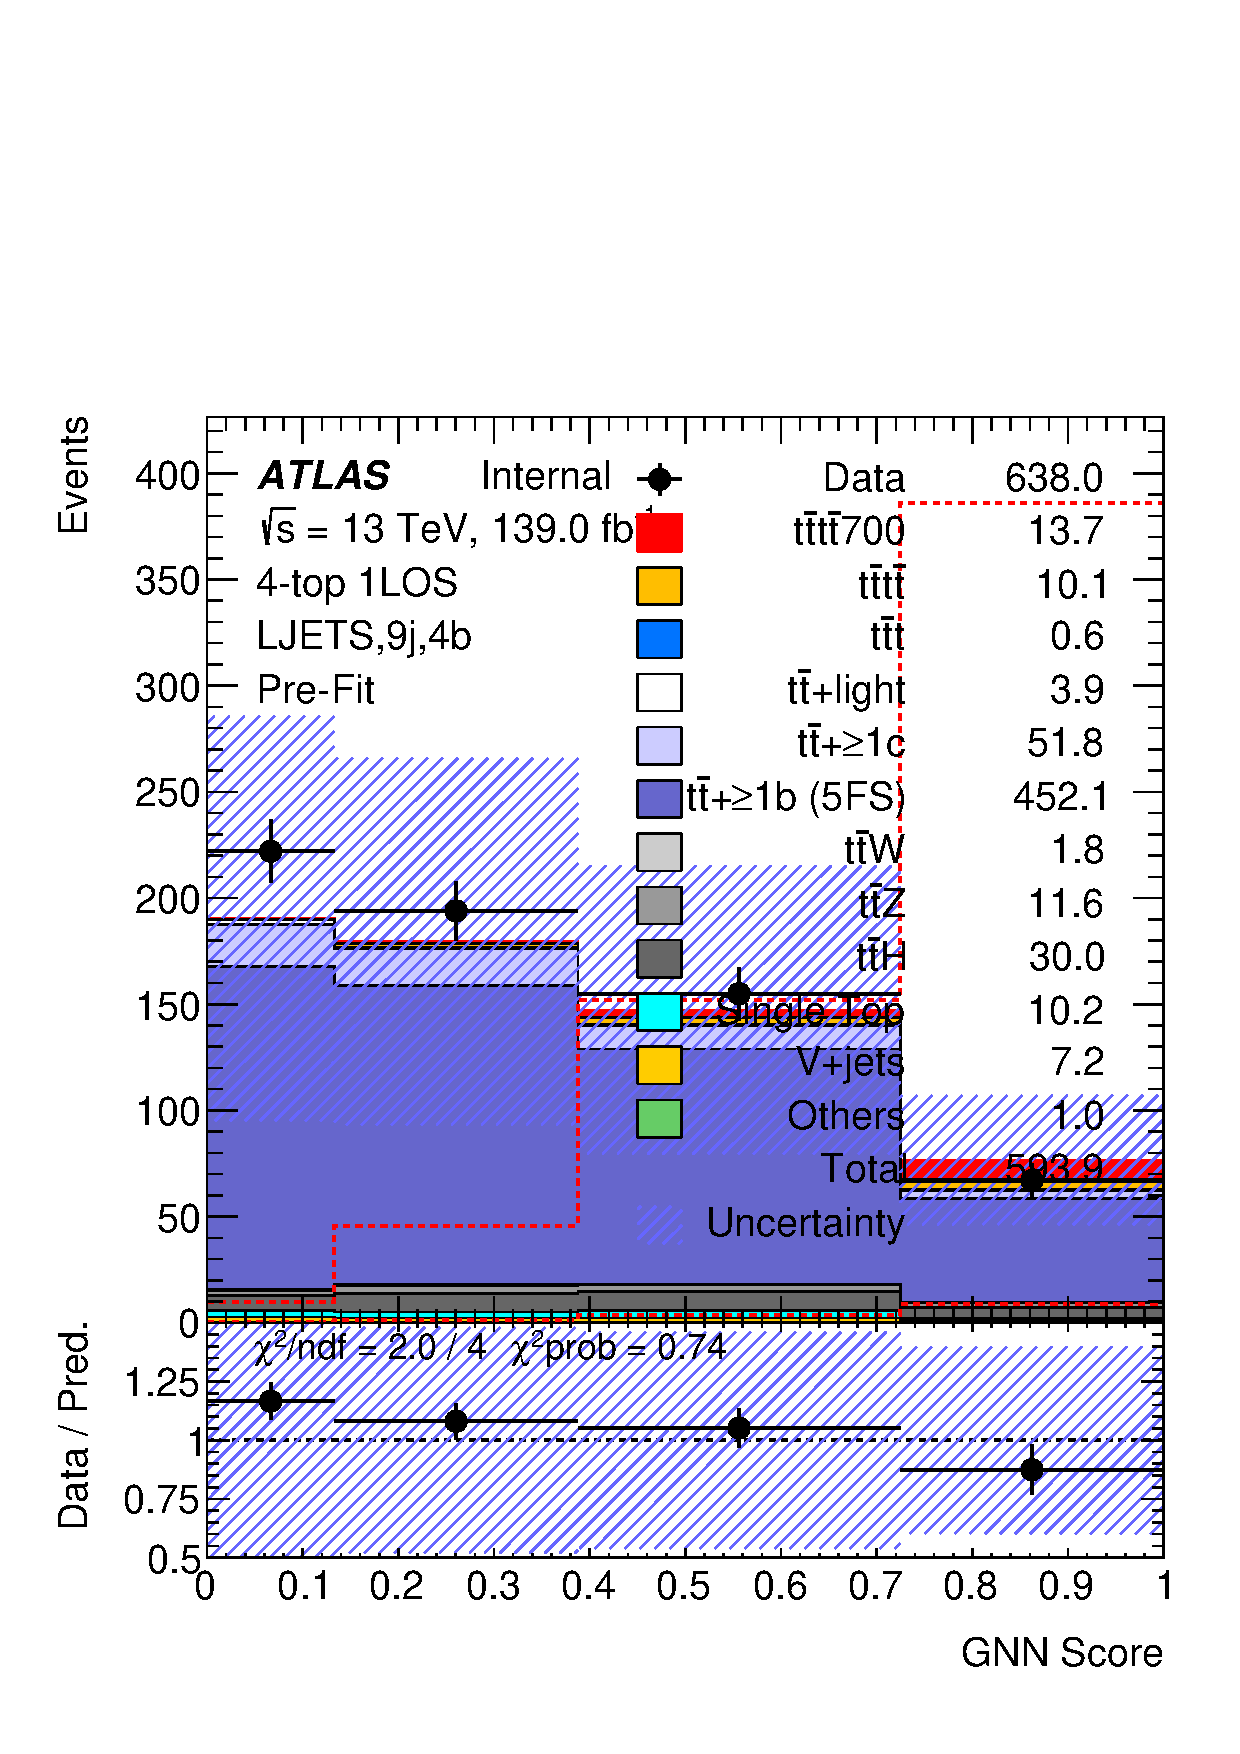
\includegraphics[width=0.23 \textwidth]{figures/fits/GNN/700/all/data_unblindedBonly/Plots/ljets_9j4b.pdf} &
        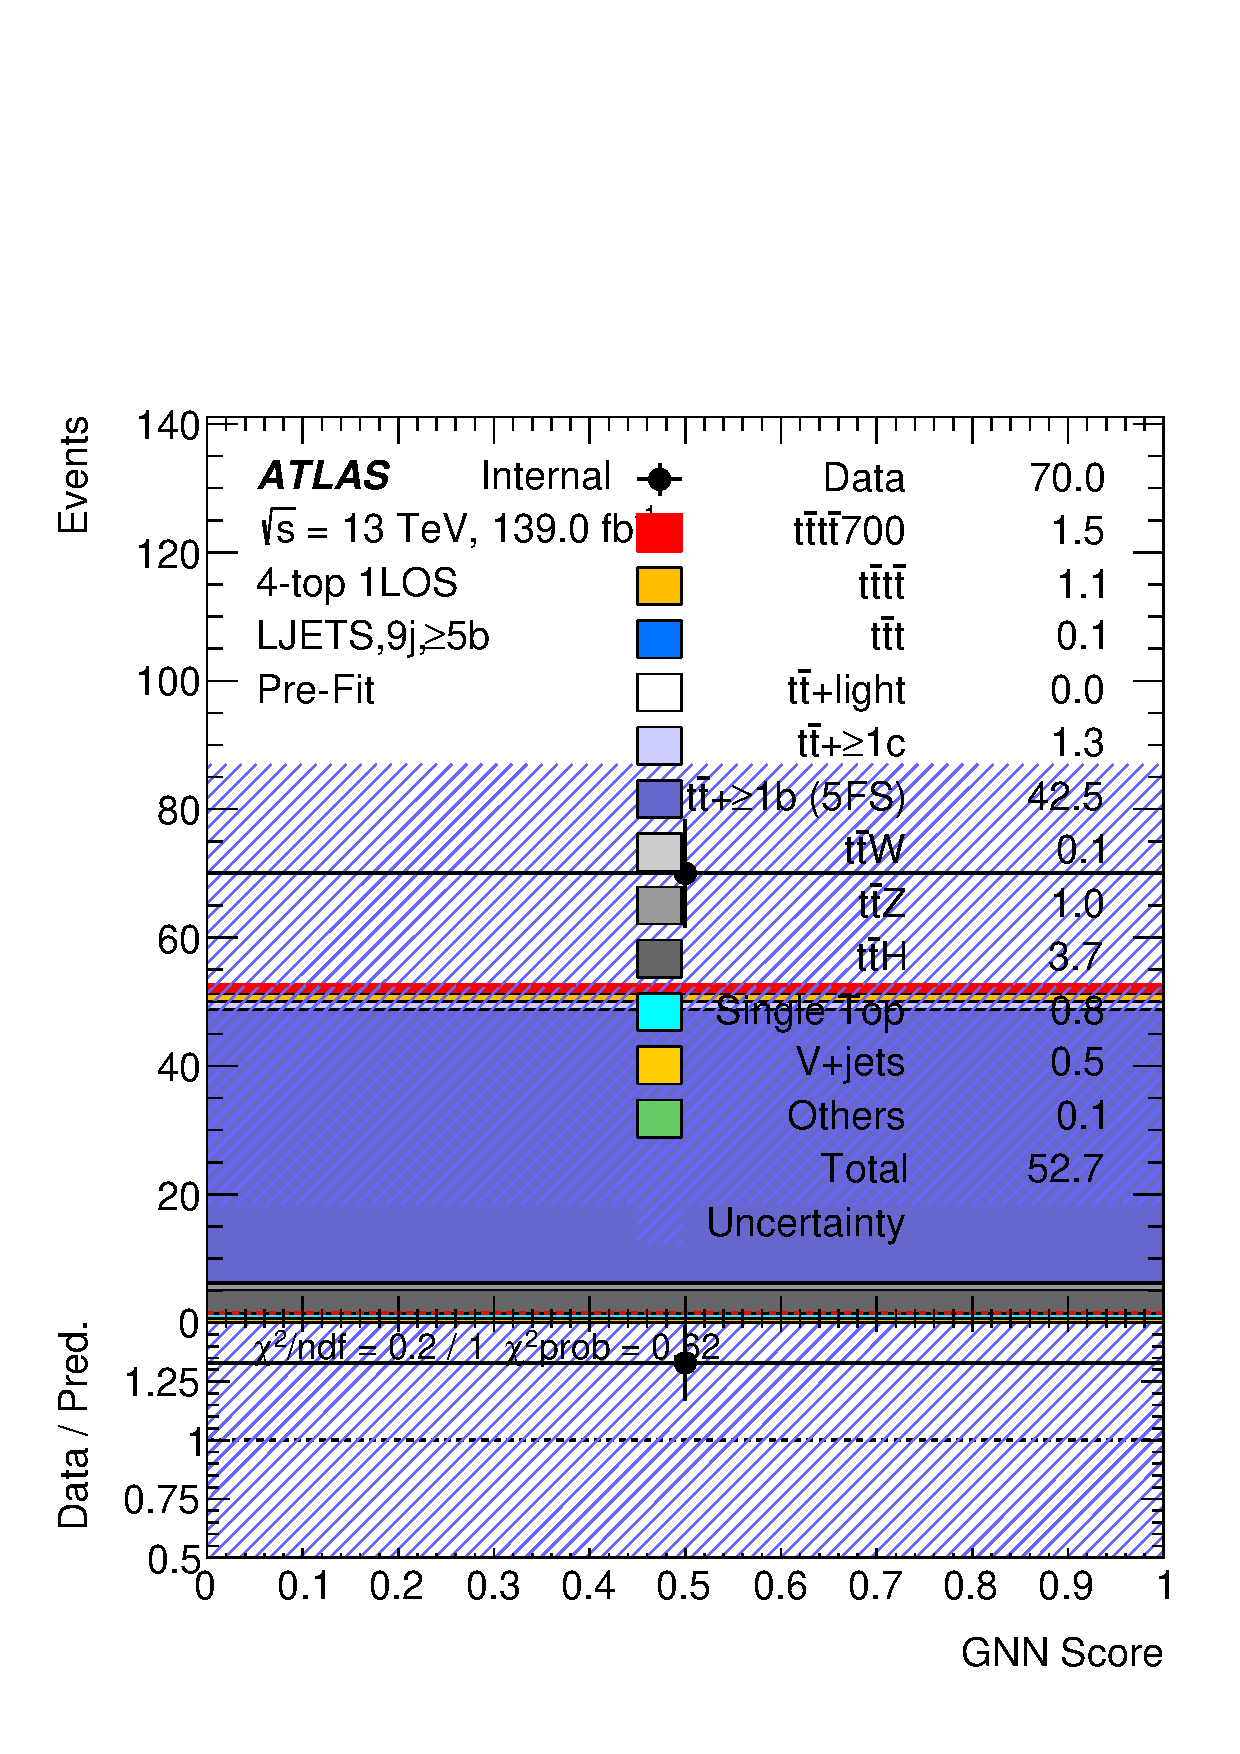
\includegraphics[width=0.23 \textwidth]{figures/fits/GNN/700/all/data_unblindedBonly/Plots/ljets_9jge5b.pdf} \\

        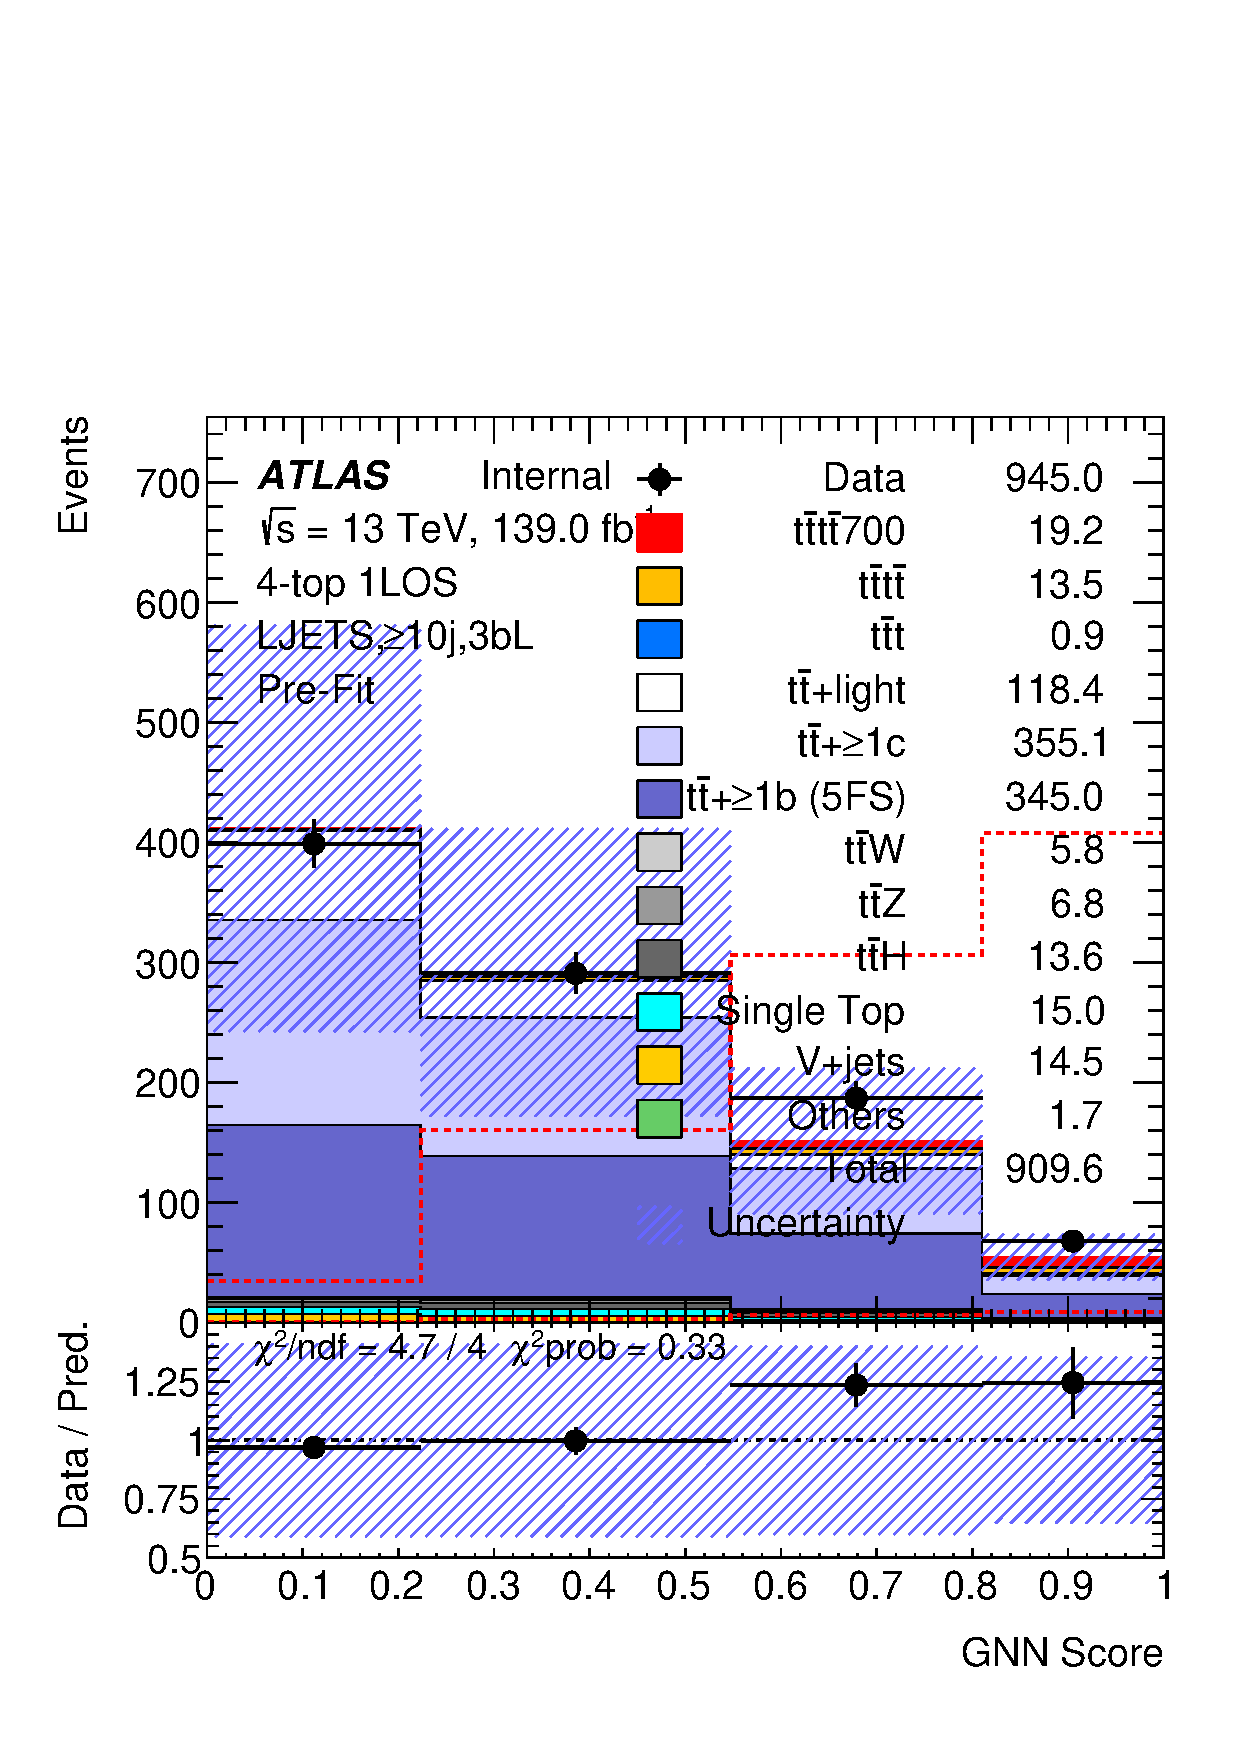
\includegraphics[width=0.23 \textwidth]{figures/fits/GNN/700/all/data_unblindedBonly/Plots/ljets_ge10j3bL.pdf} &
        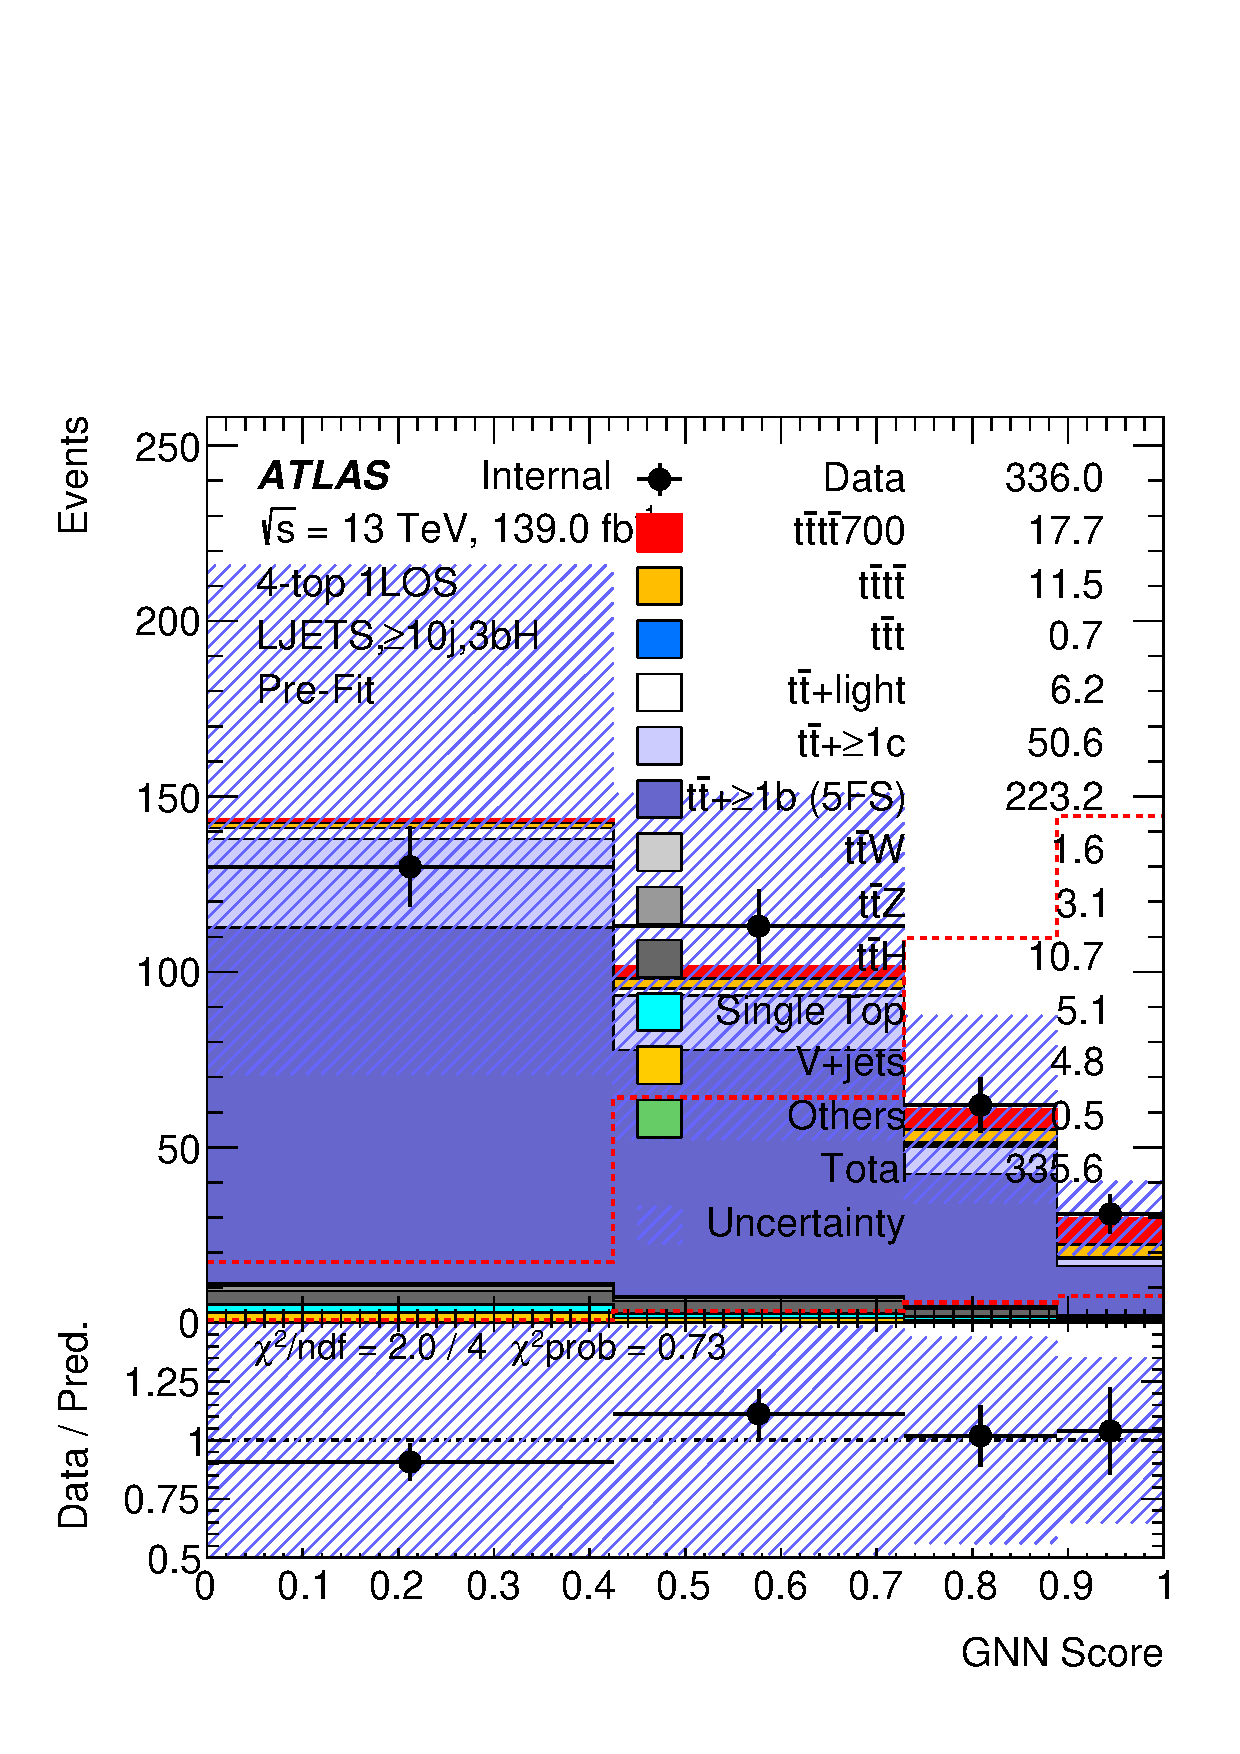
\includegraphics[width=0.23 \textwidth]{figures/fits/GNN/700/all/data_unblindedBonly/Plots/ljets_ge10j3bH.pdf} &
        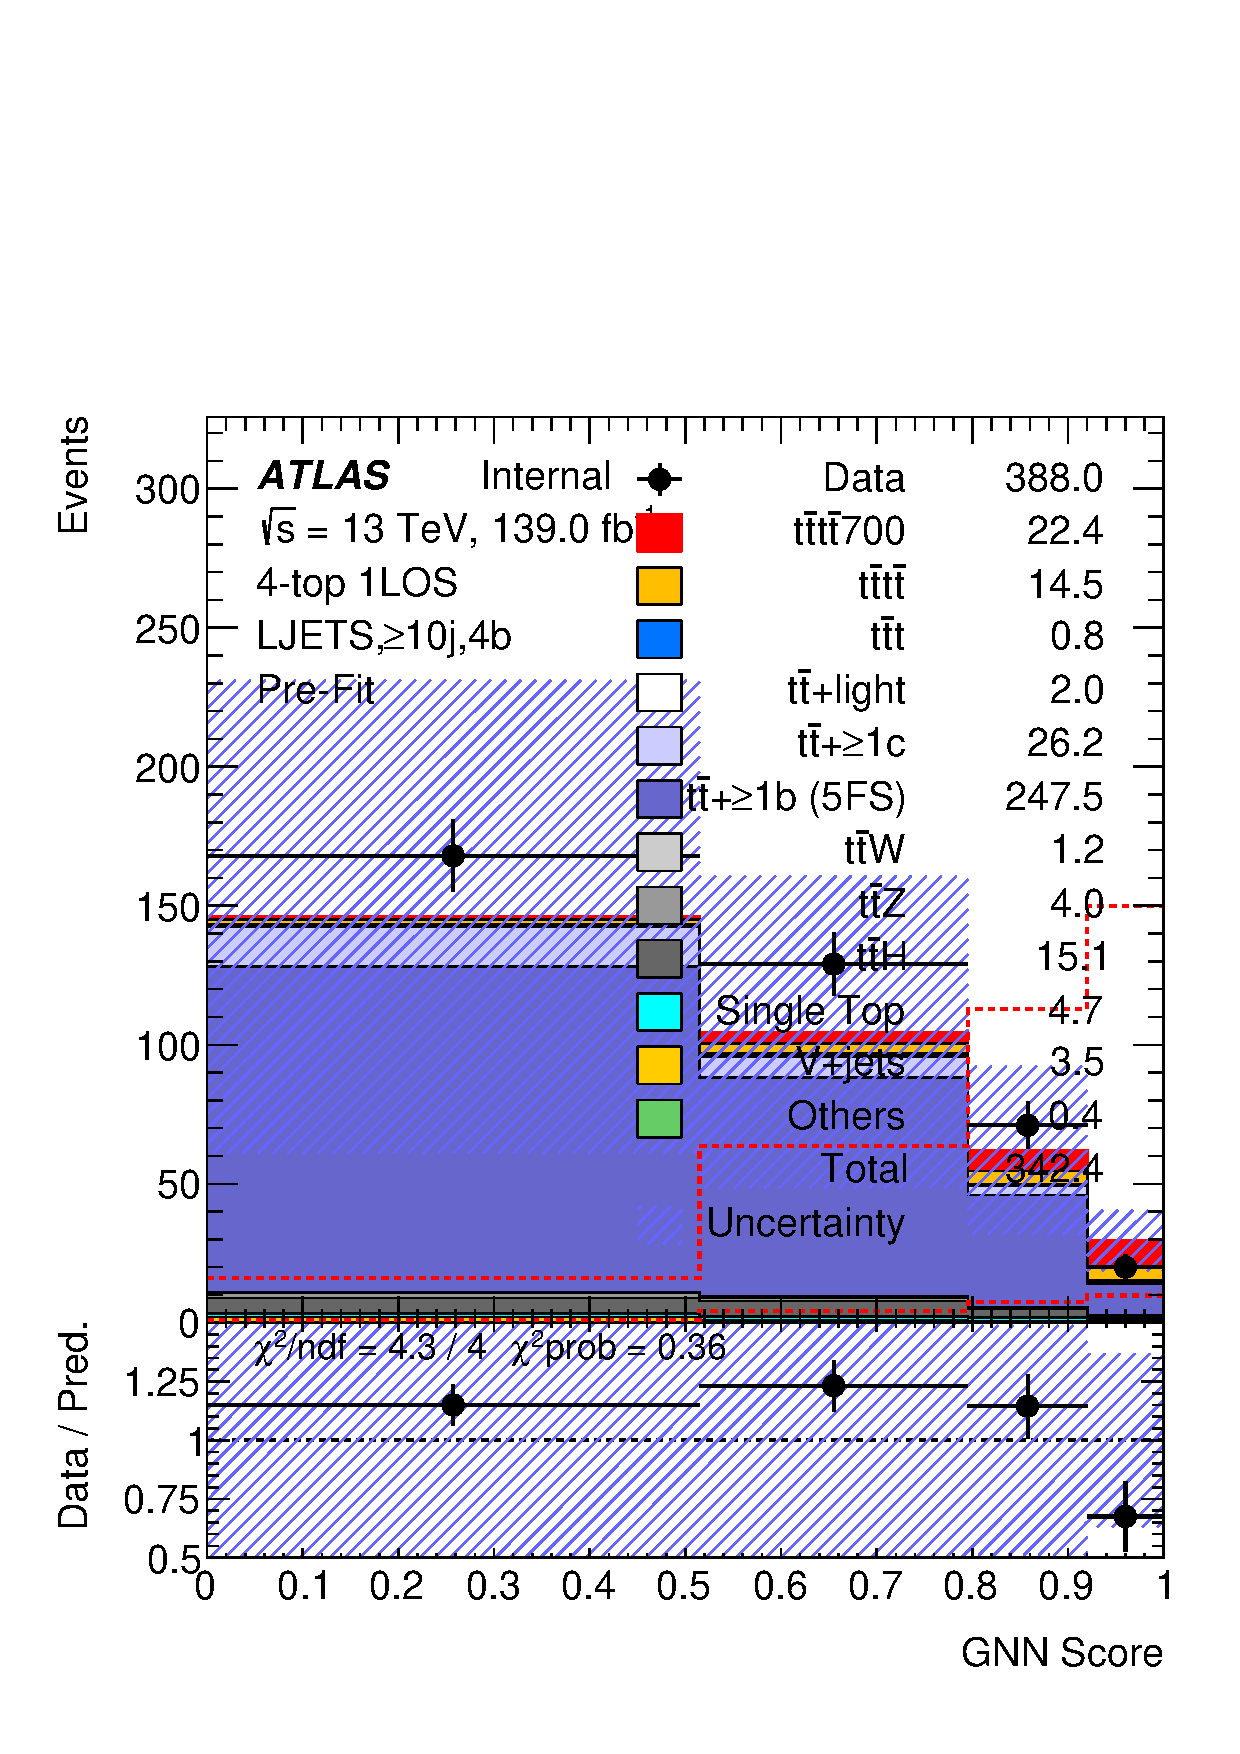
\includegraphics[width=0.23 \textwidth]{figures/fits/GNN/700/all/data_unblindedBonly/Plots/ljets_ge10j4b.pdf} &
        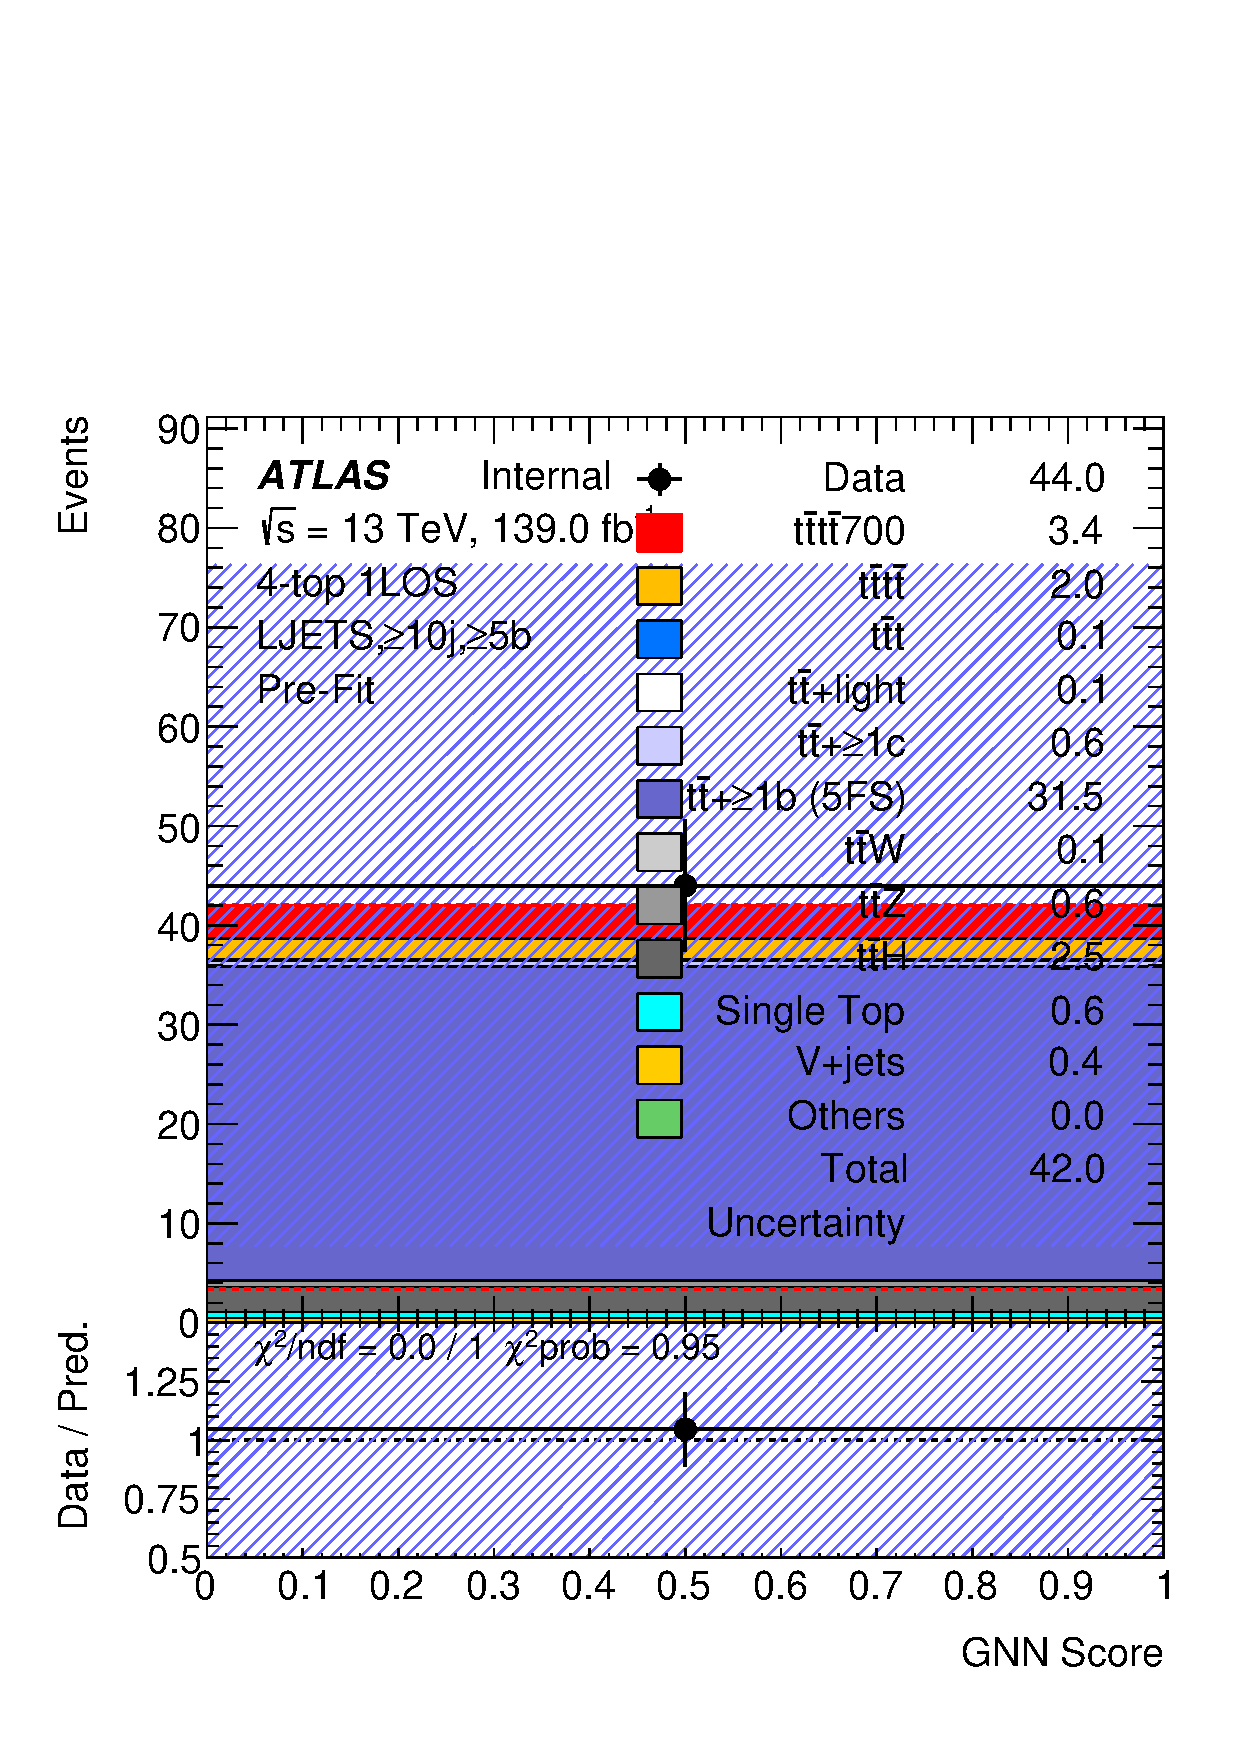
\includegraphics[width=0.23 \textwidth]{figures/fits/GNN/700/all/data_unblindedBonly/Plots/ljets_ge10jge5b.pdf} \\
        \end{tabular}
        \caption{\label{fig:Prefit_Yields_1L_700GeV}Pre-fit distributions for 1L signal regions associated with different signal and background samples, compared with data yields for mH = 700 GeV.}
\end{center}
\end{figure}

\begin{figure}[htbp!]
        \begin{center} \setlength{\tabcolsep}{2.5pt}\footnotesize
        \begin{tabular}{ccc}

        &
        &
        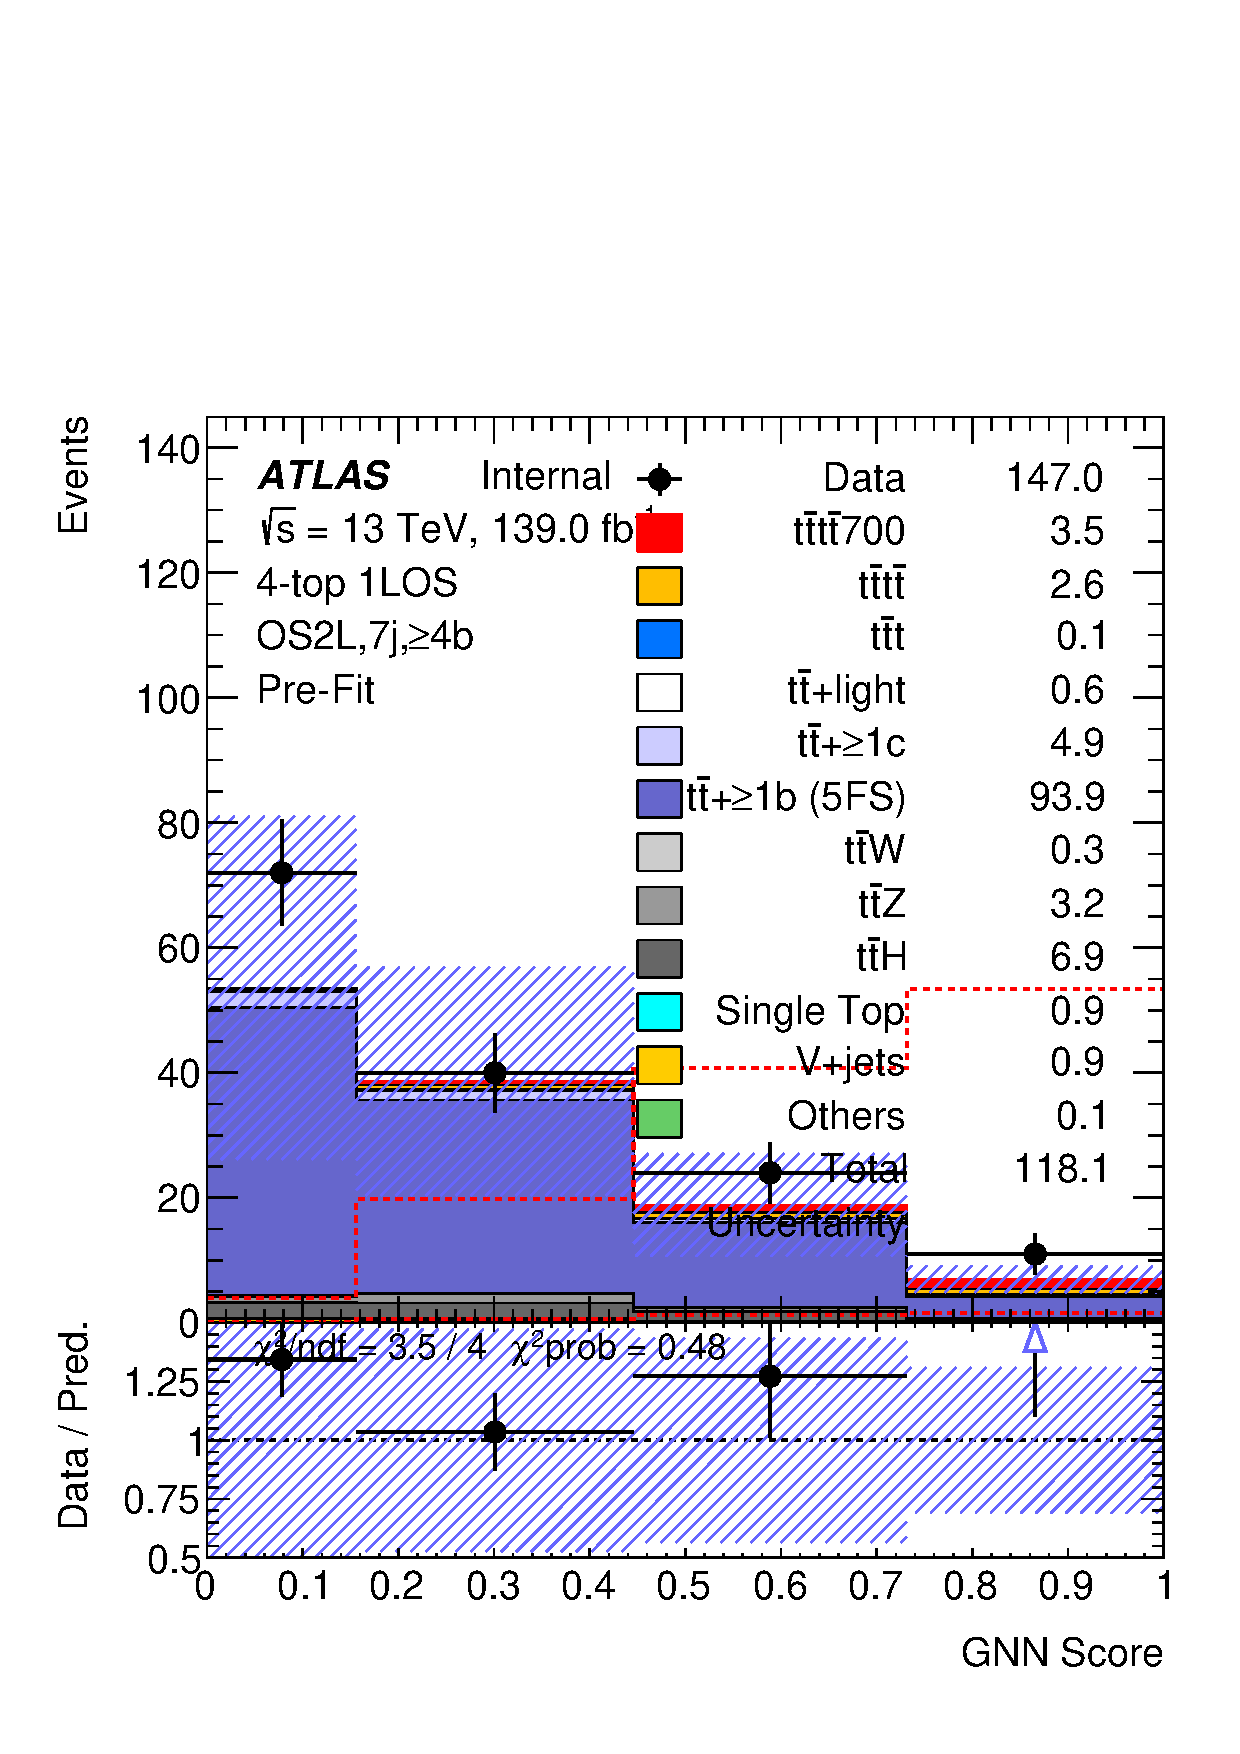
\includegraphics[width=0.31 \textwidth]{figures/fits/GNN/700/all/data_unblindedBonly/Plots/os2l_7jge4b.pdf} \\

        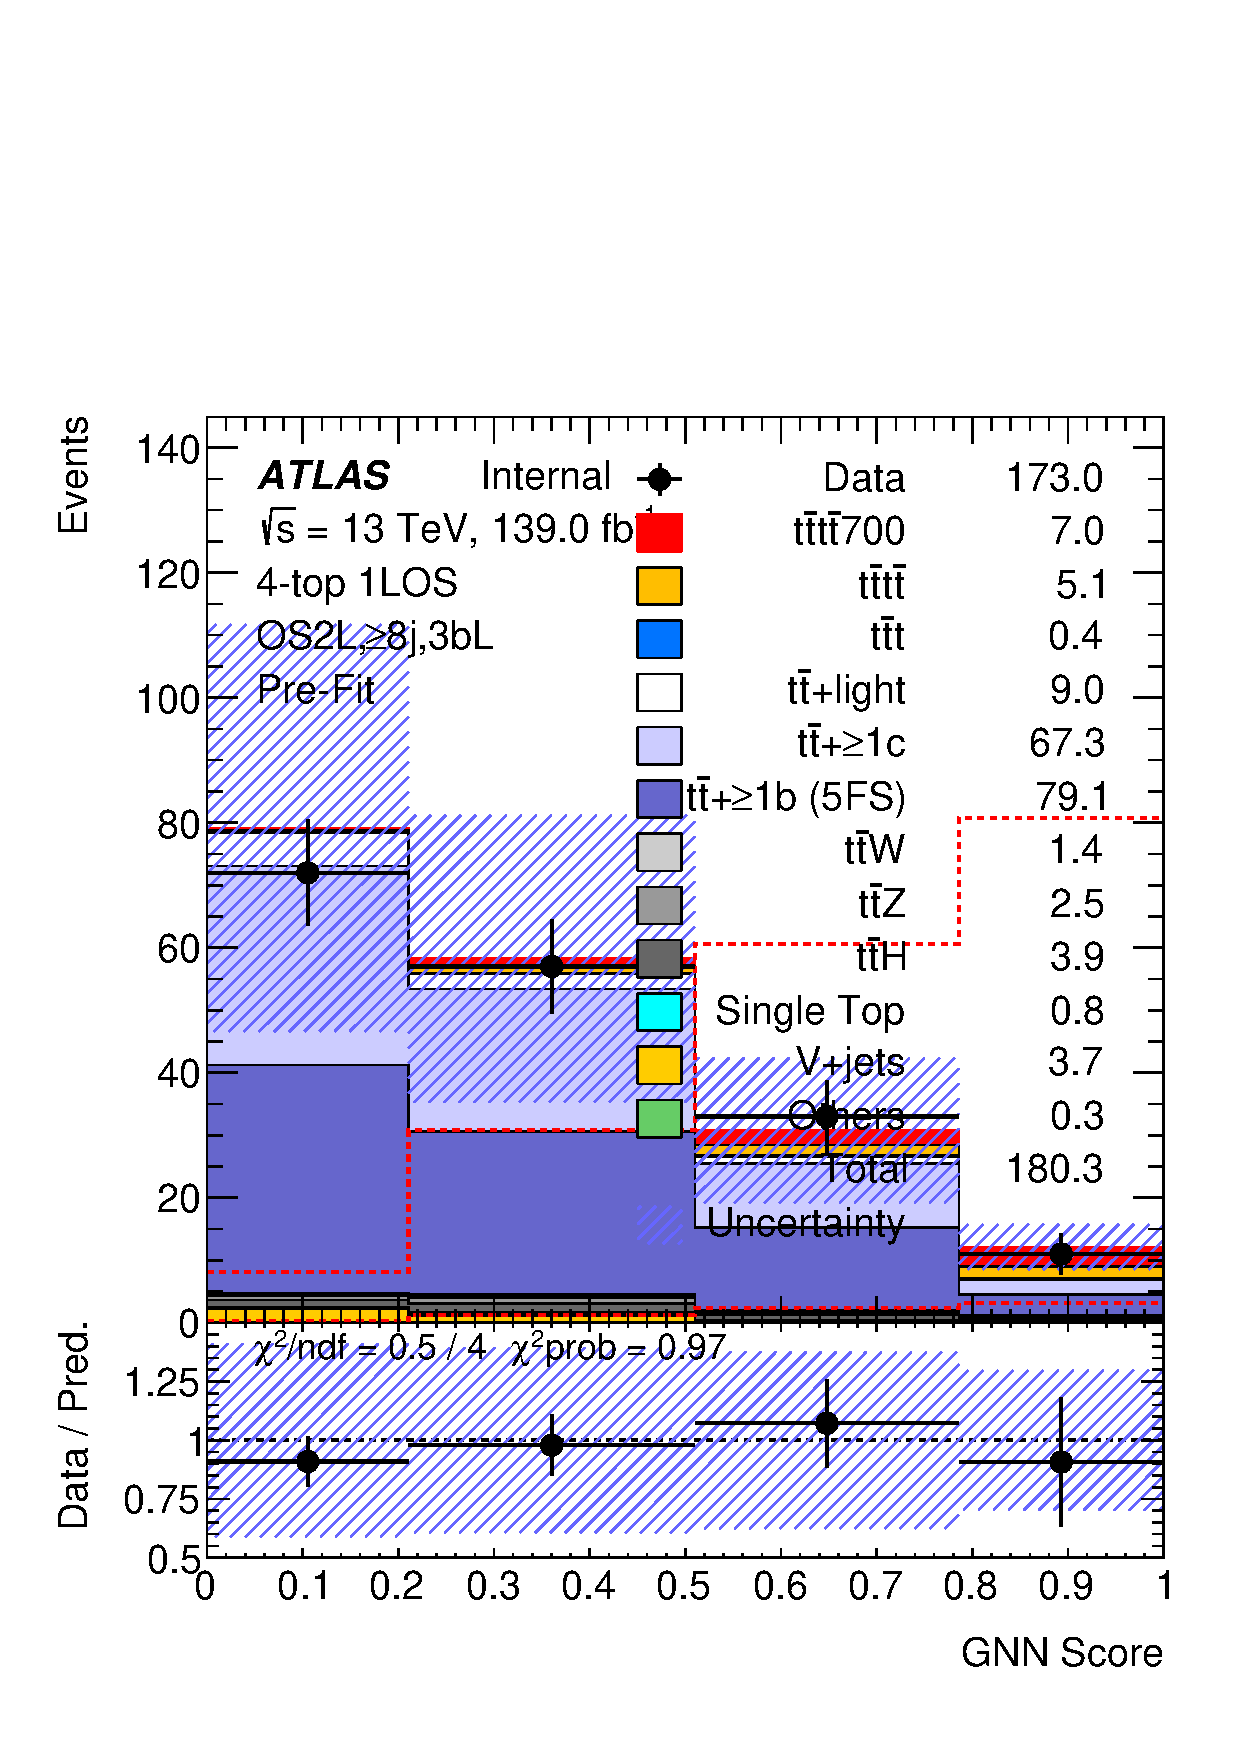
\includegraphics[width=0.31 \textwidth]{figures/fits/GNN/700/all/data_unblindedBonly/Plots/os2l_ge8j3bL.pdf} &
        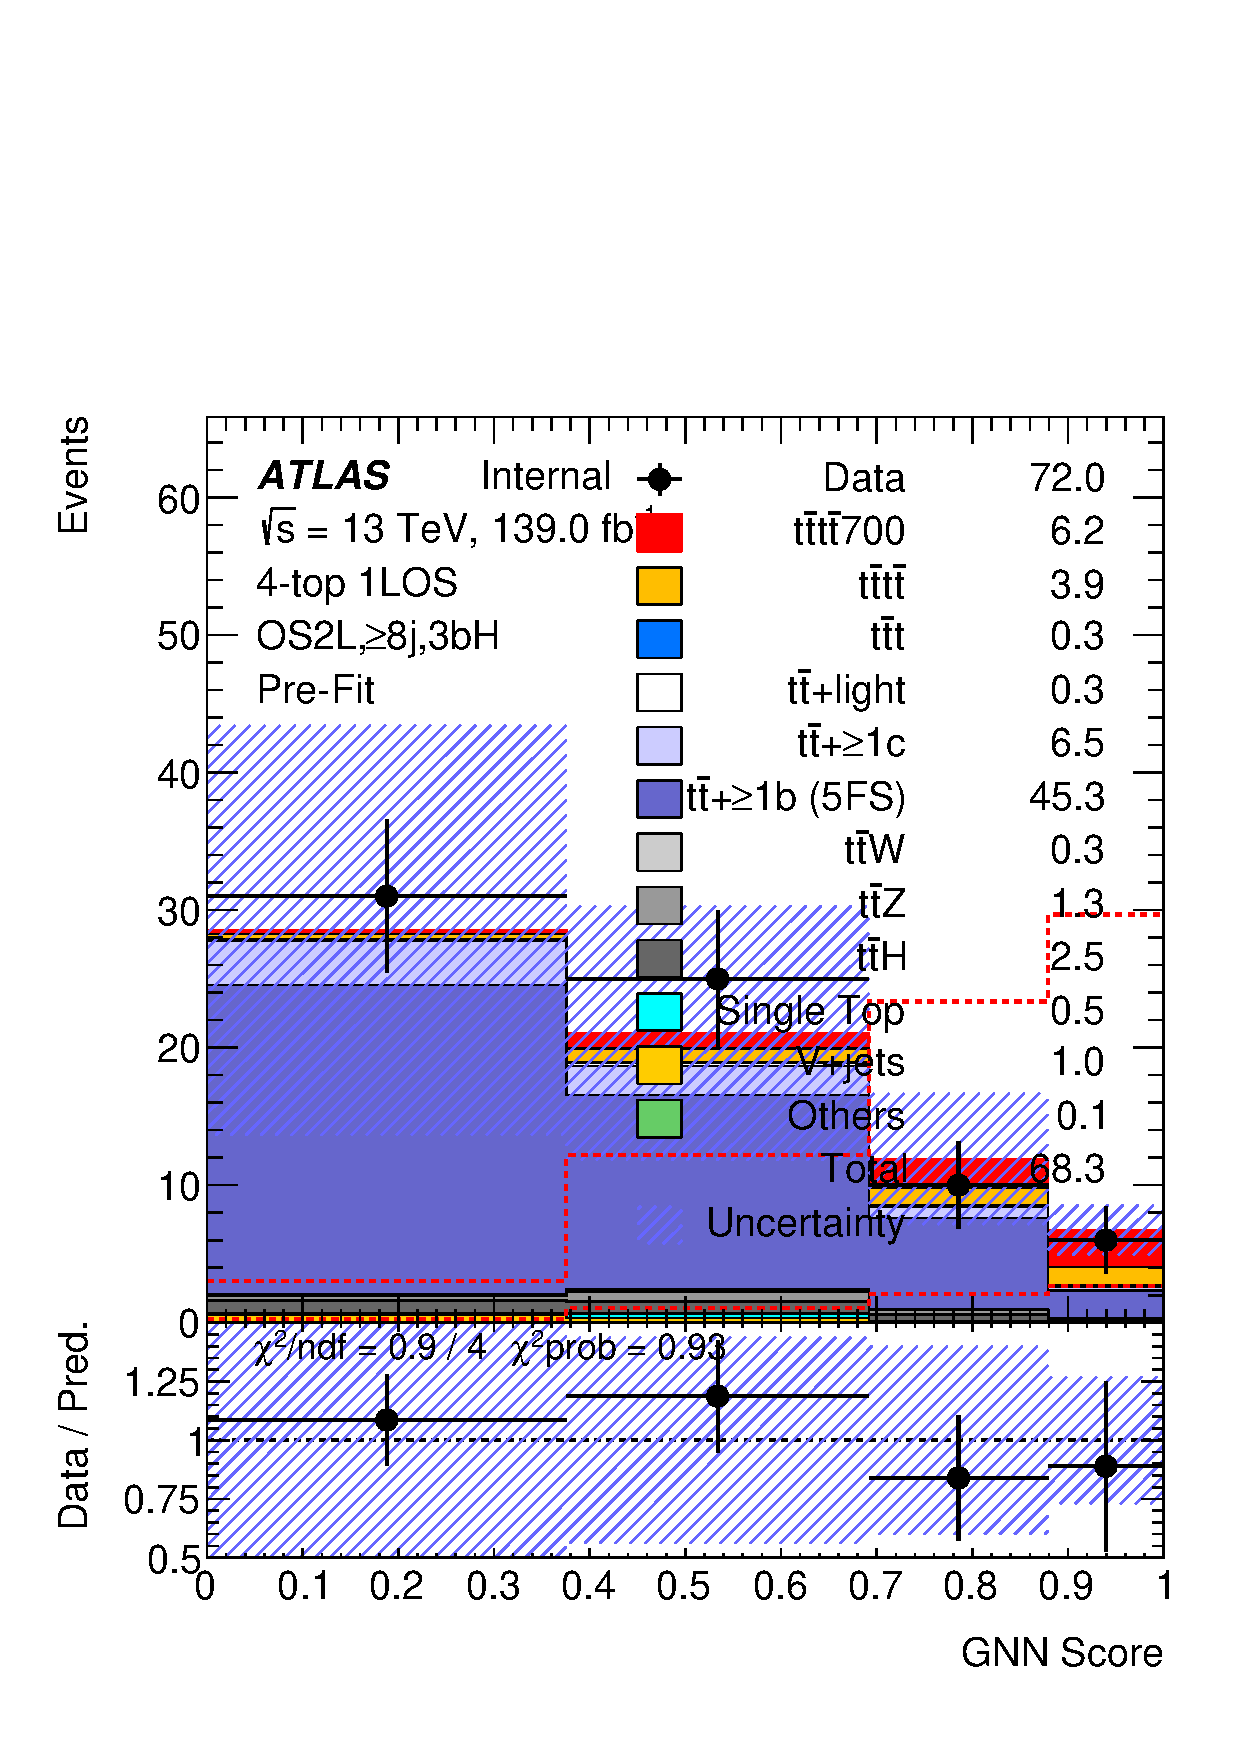
\includegraphics[width=0.31 \textwidth]{figures/fits/GNN/700/all/data_unblindedBonly/Plots/os2l_ge8j3bH.pdf} &
        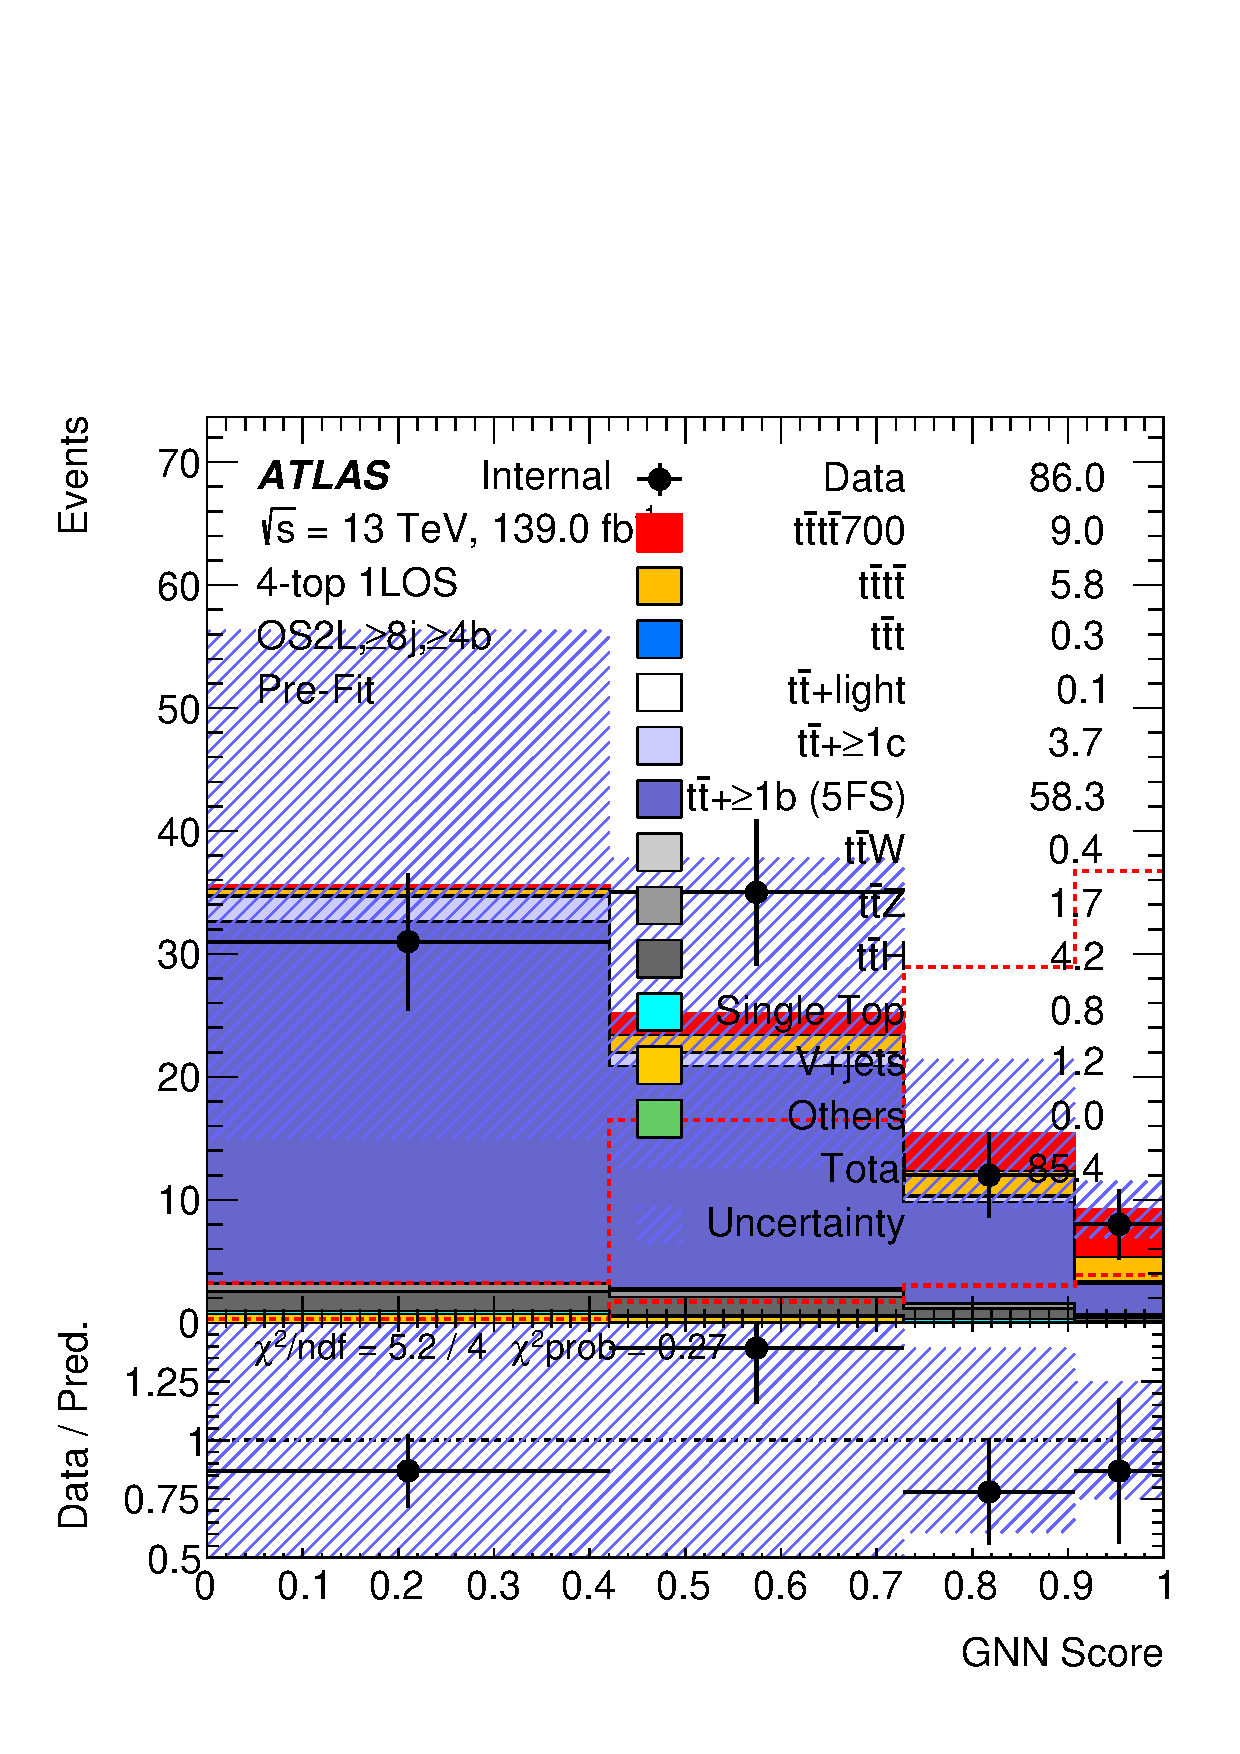
\includegraphics[width=0.31 \textwidth]{figures/fits/GNN/700/all/data_unblindedBonly/Plots/os2l_ge8jge4b.pdf} \\
        \end{tabular}
        \caption{\label{fig:Prefit_Yields_2L_700GeV}Pre-fit distributions for 2LOS signal regions associated with different signal and background samples, compared with data yields for mH = 700 GeV.}
\end{center}
\end{figure}

\begin{figure}[htbp!]
        \begin{center} \setlength{\tabcolsep}{2.5pt}\footnotesize
        \begin{tabular}{cccc}
        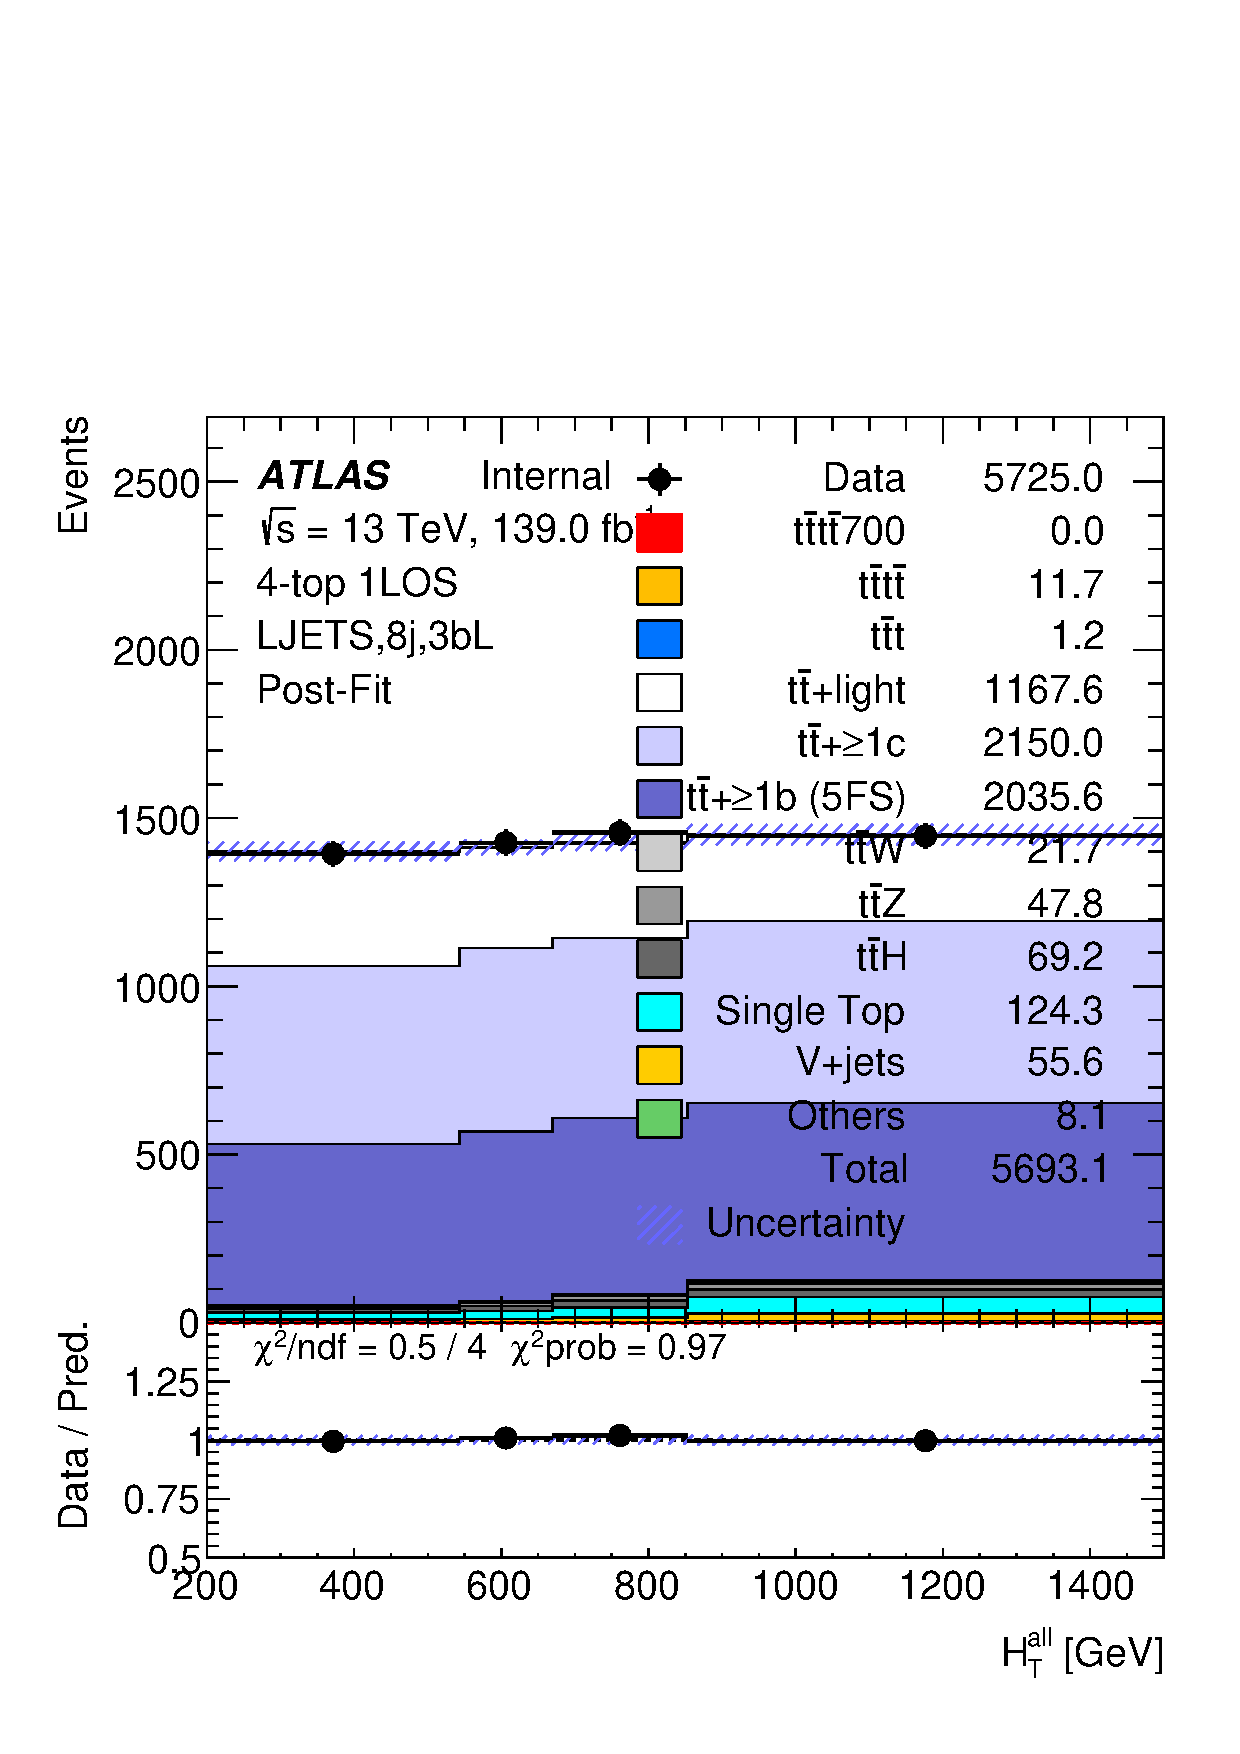
\includegraphics[width=0.23 \textwidth]{figures/fits/GNN/700/all/data_unblindedBonly/Plots/ljets_8j3bL_postFit.pdf} &
        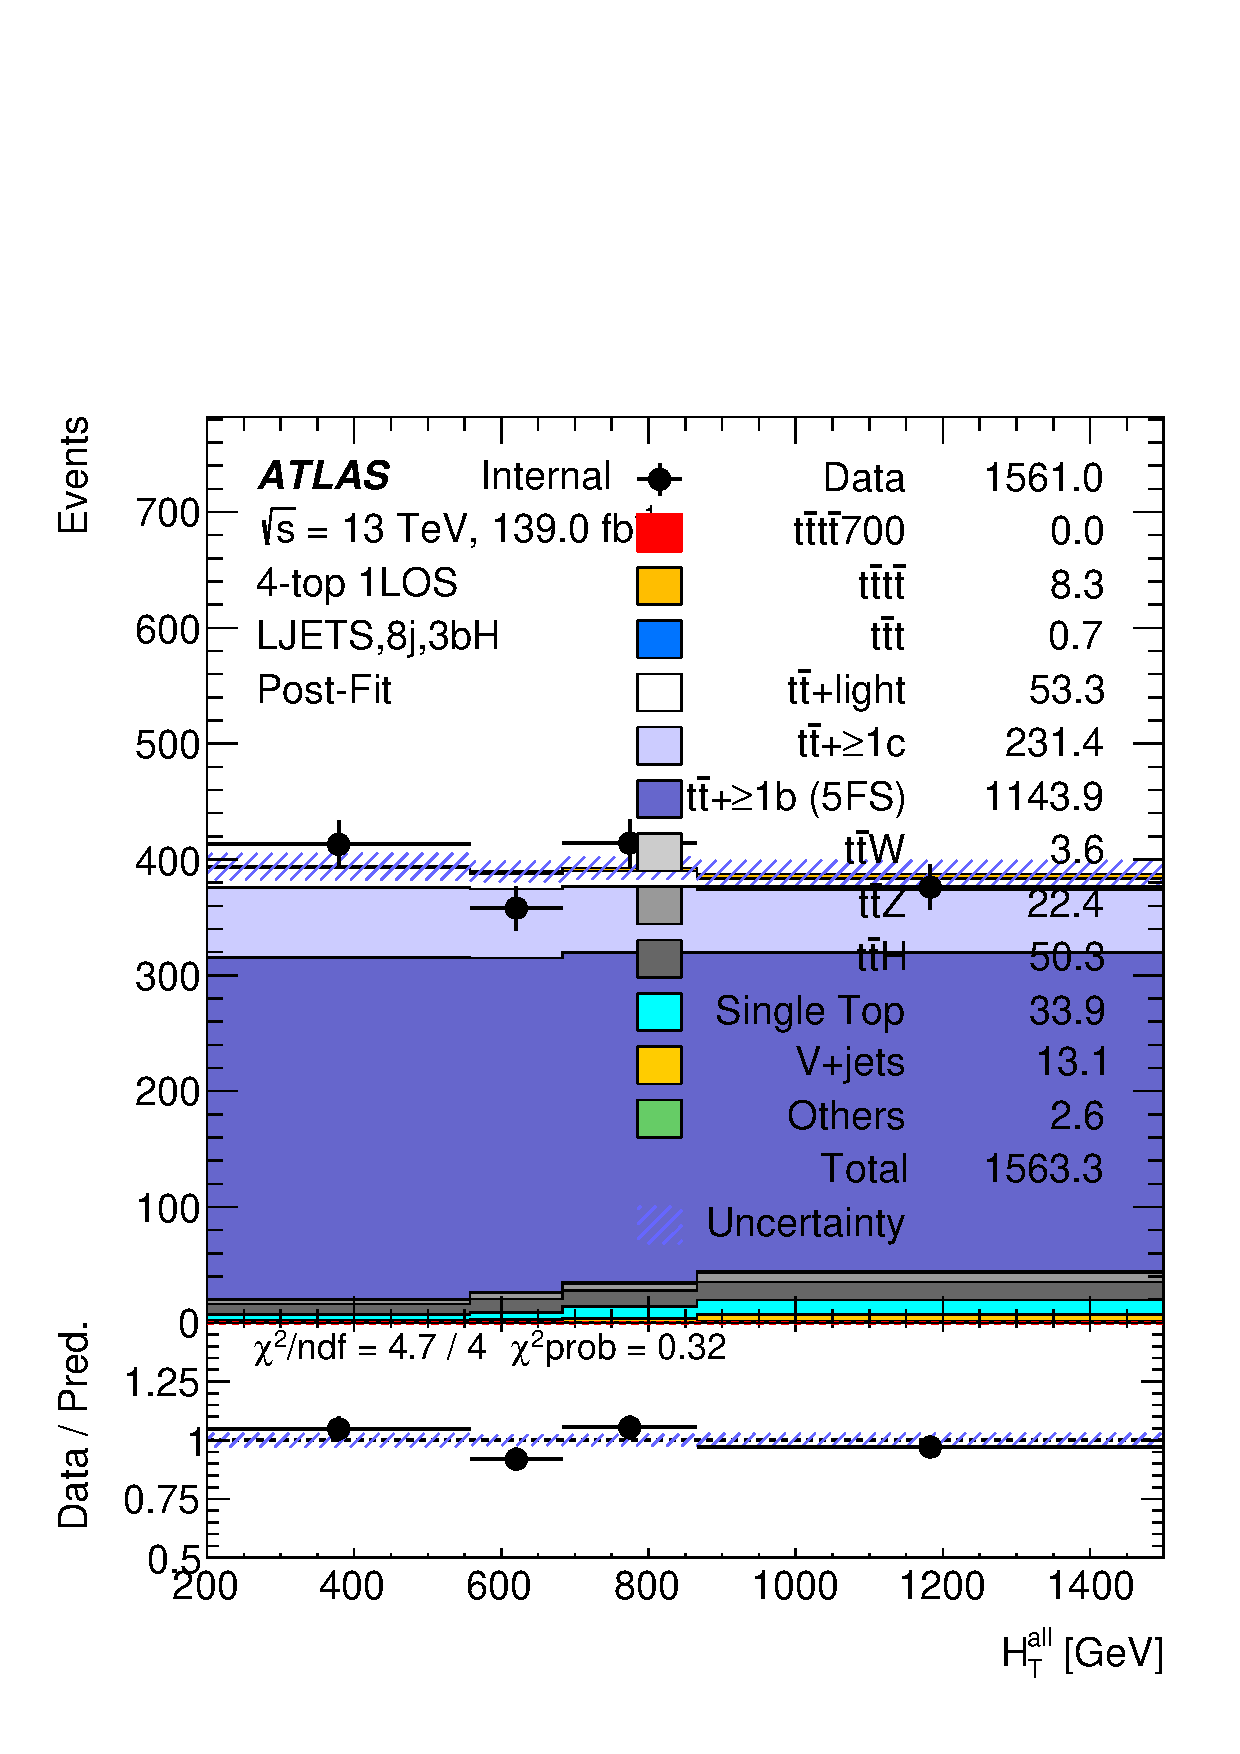
\includegraphics[width=0.23 \textwidth]{figures/fits/GNN/700/all/data_unblindedBonly/Plots/ljets_8j3bH_postFit.pdf} &
        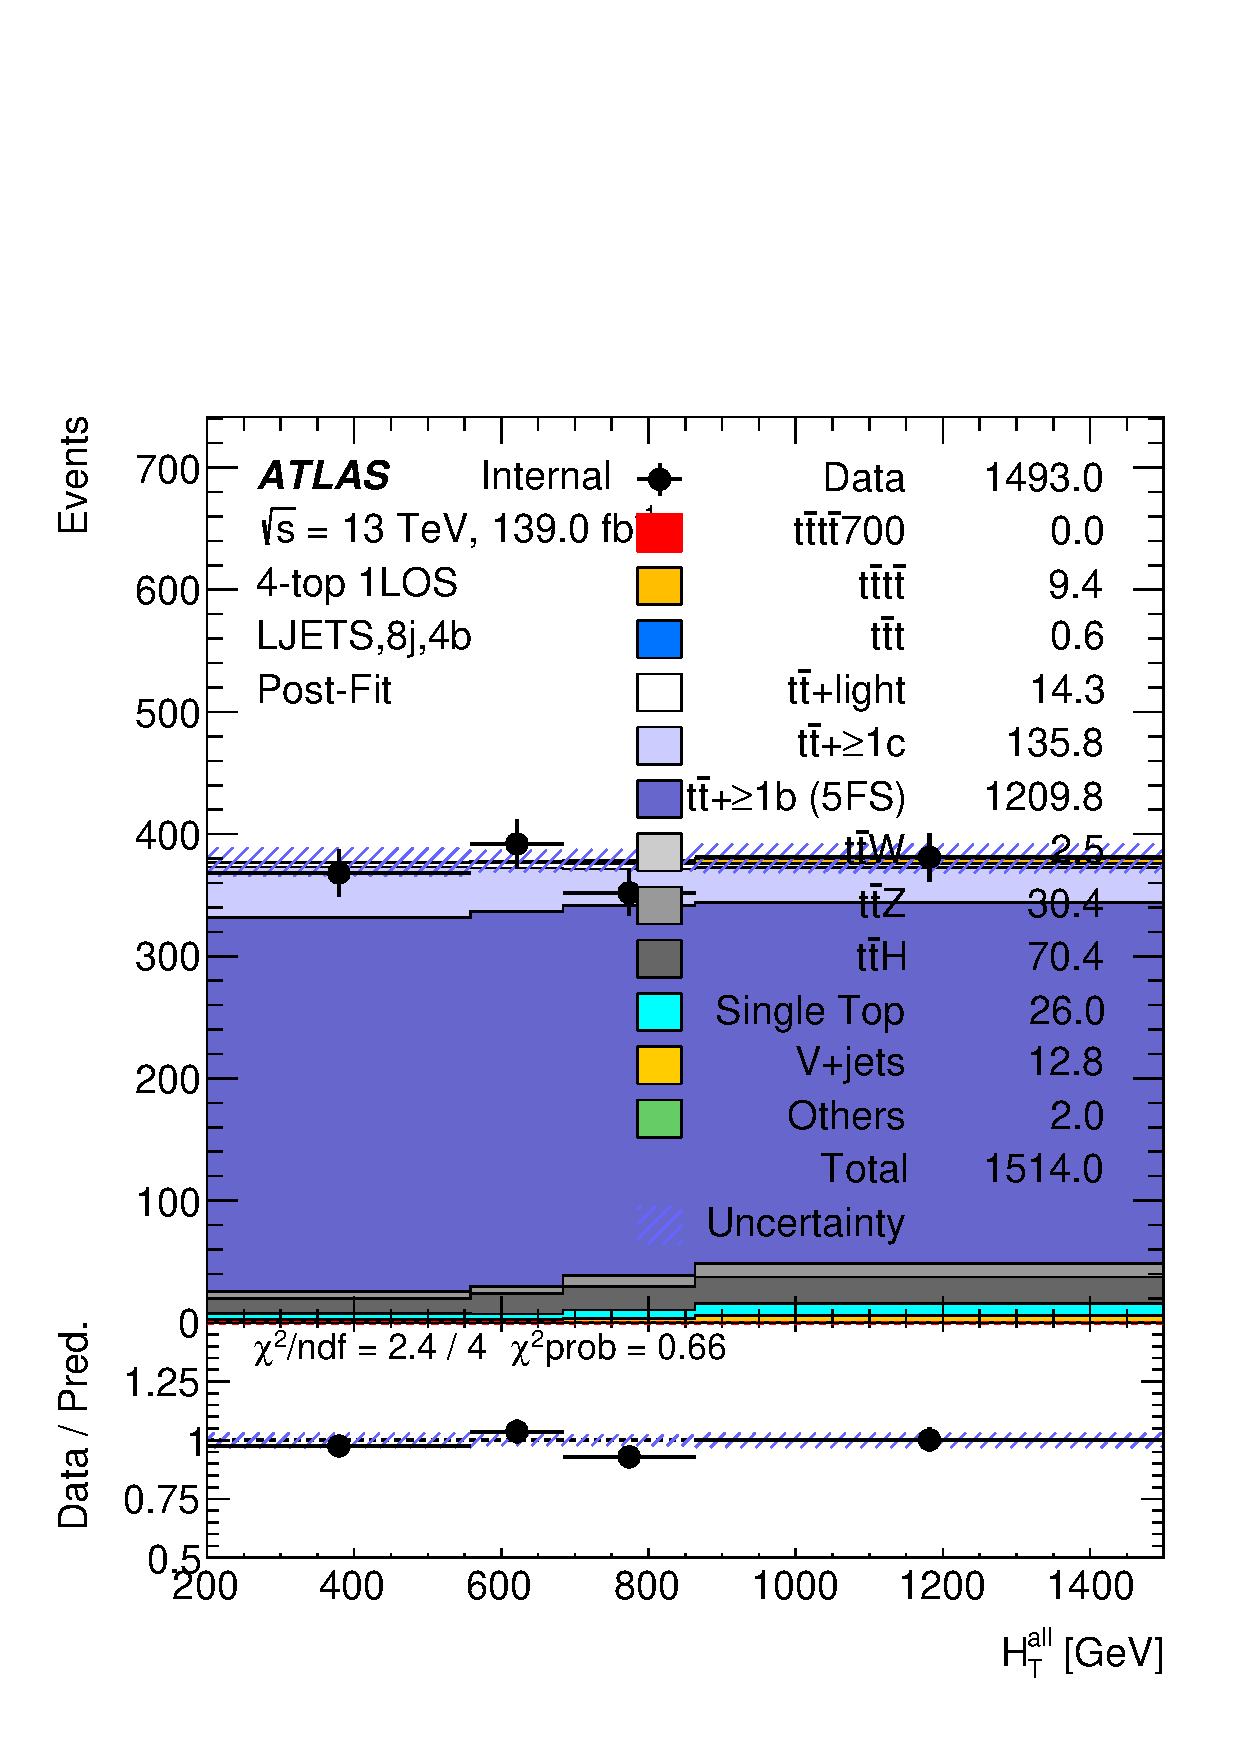
\includegraphics[width=0.23 \textwidth]{figures/fits/GNN/700/all/data_unblindedBonly/Plots/ljets_8j4b_postFit.pdf} &
        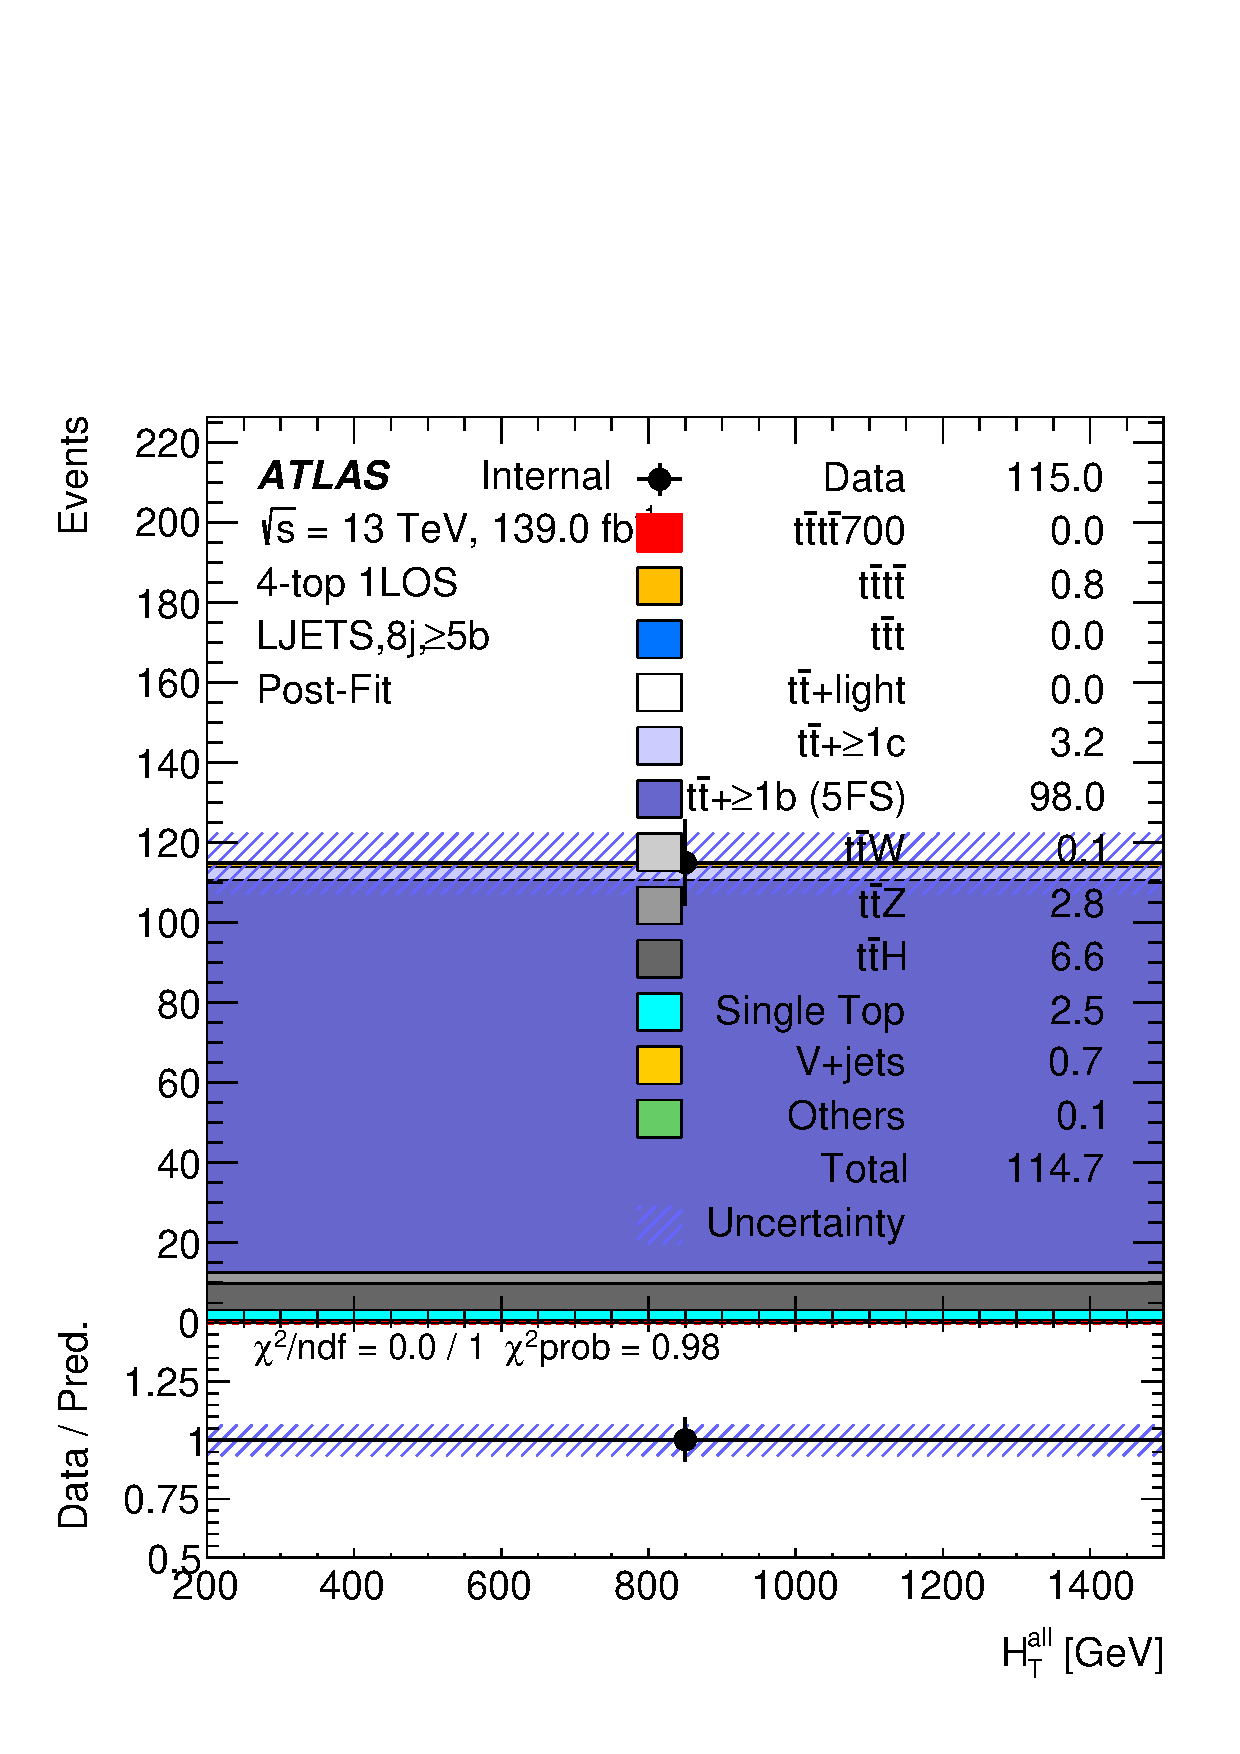
\includegraphics[width=0.23 \textwidth]{figures/fits/GNN/700/all/data_unblindedBonly/Plots/ljets_8jge5b_postFit.pdf}\\

        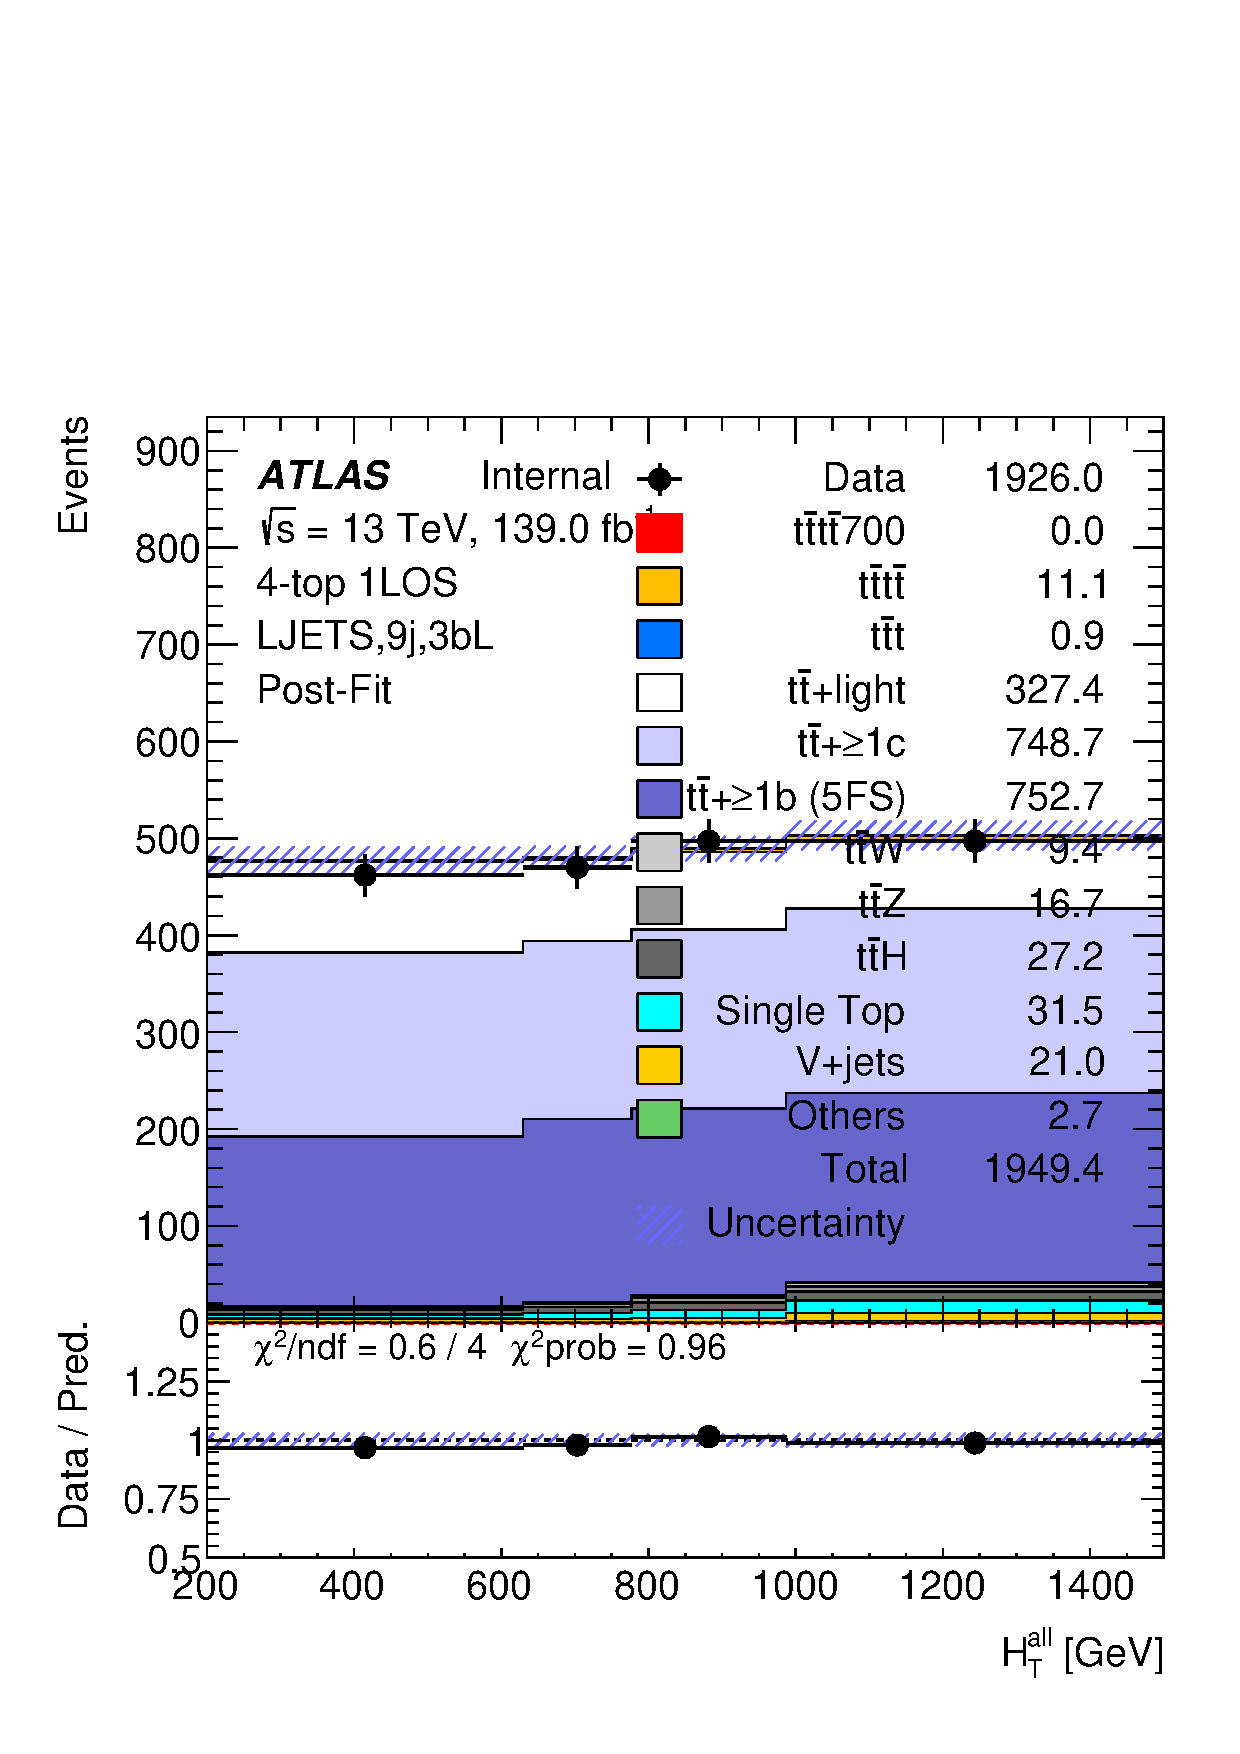
\includegraphics[width=0.23 \textwidth]{figures/fits/GNN/700/all/data_unblindedBonly/Plots/ljets_9j3bL_postFit.pdf} &
        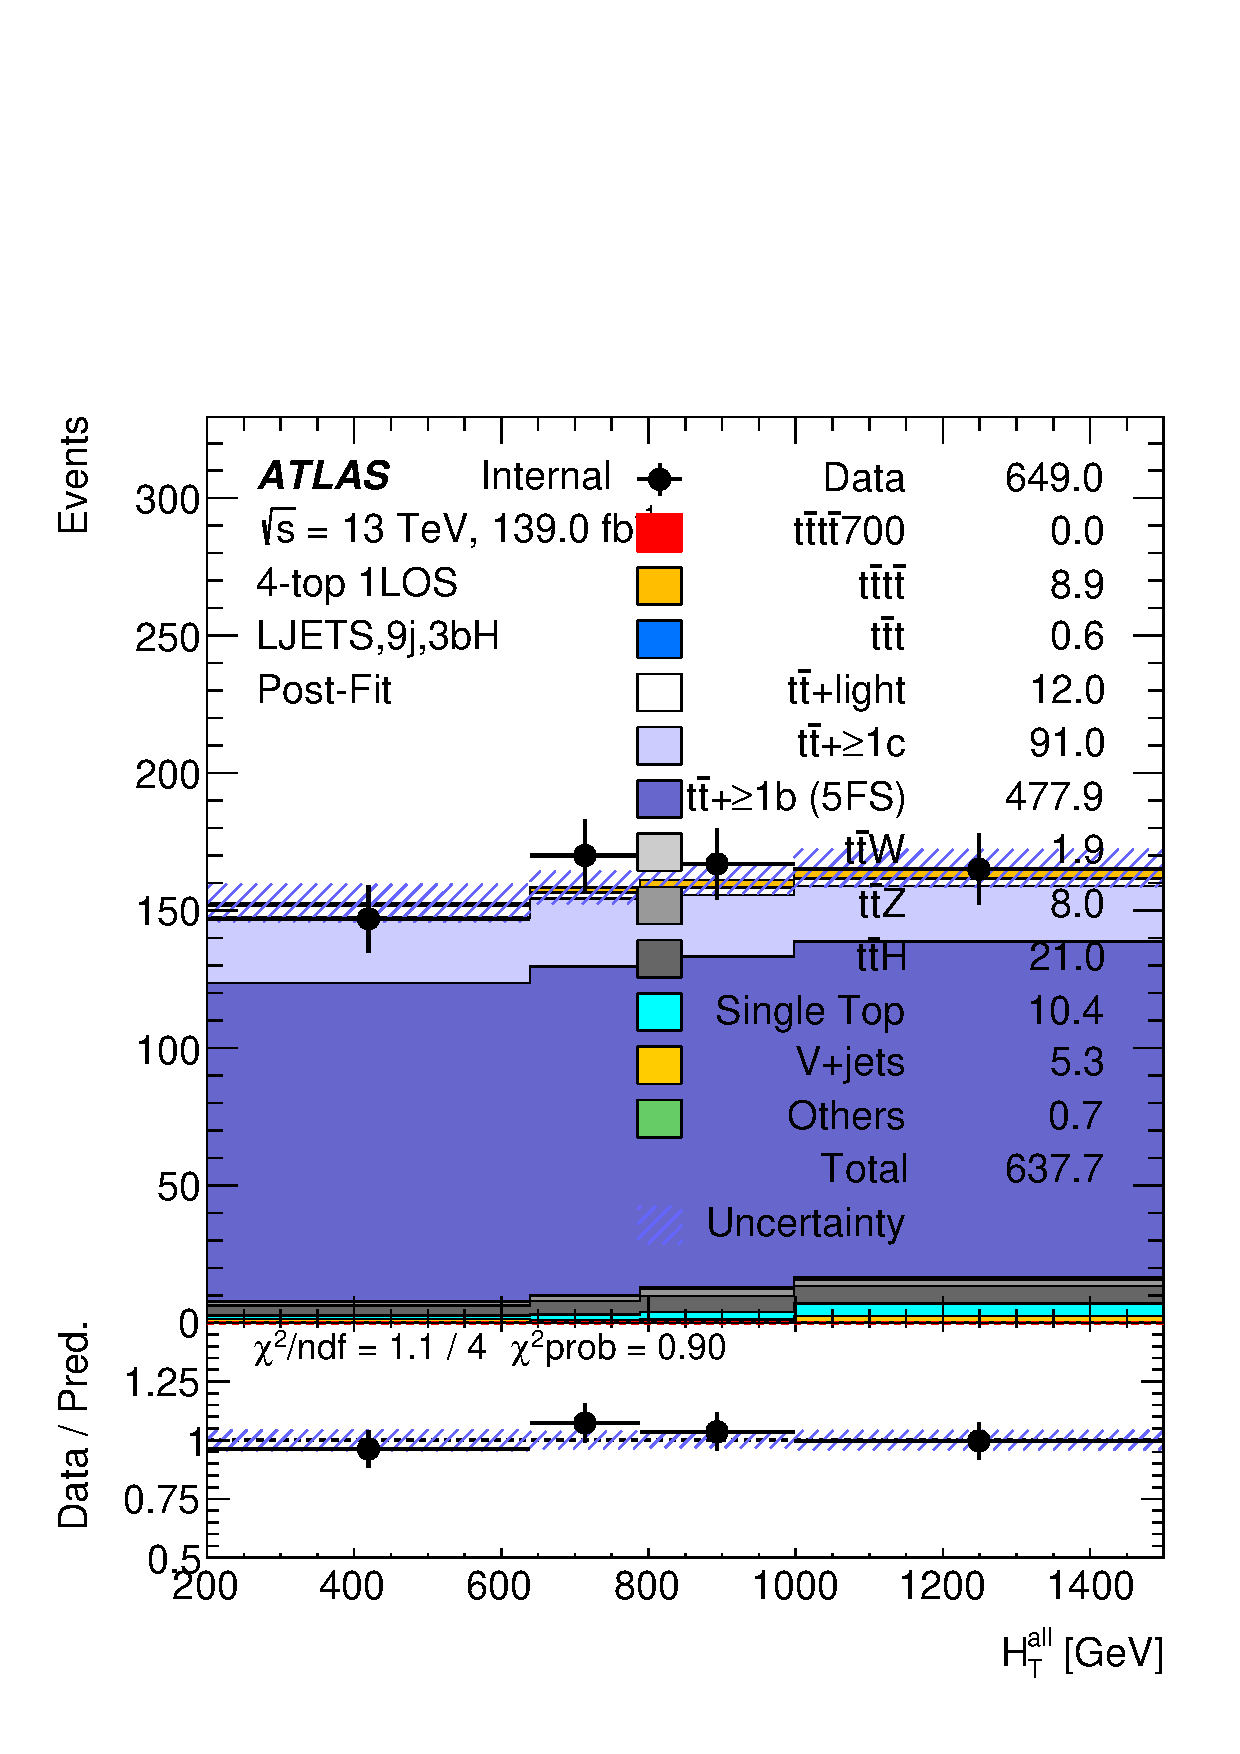
\includegraphics[width=0.23 \textwidth]{figures/fits/GNN/700/all/data_unblindedBonly/Plots/ljets_9j3bH_postFit.pdf} &
        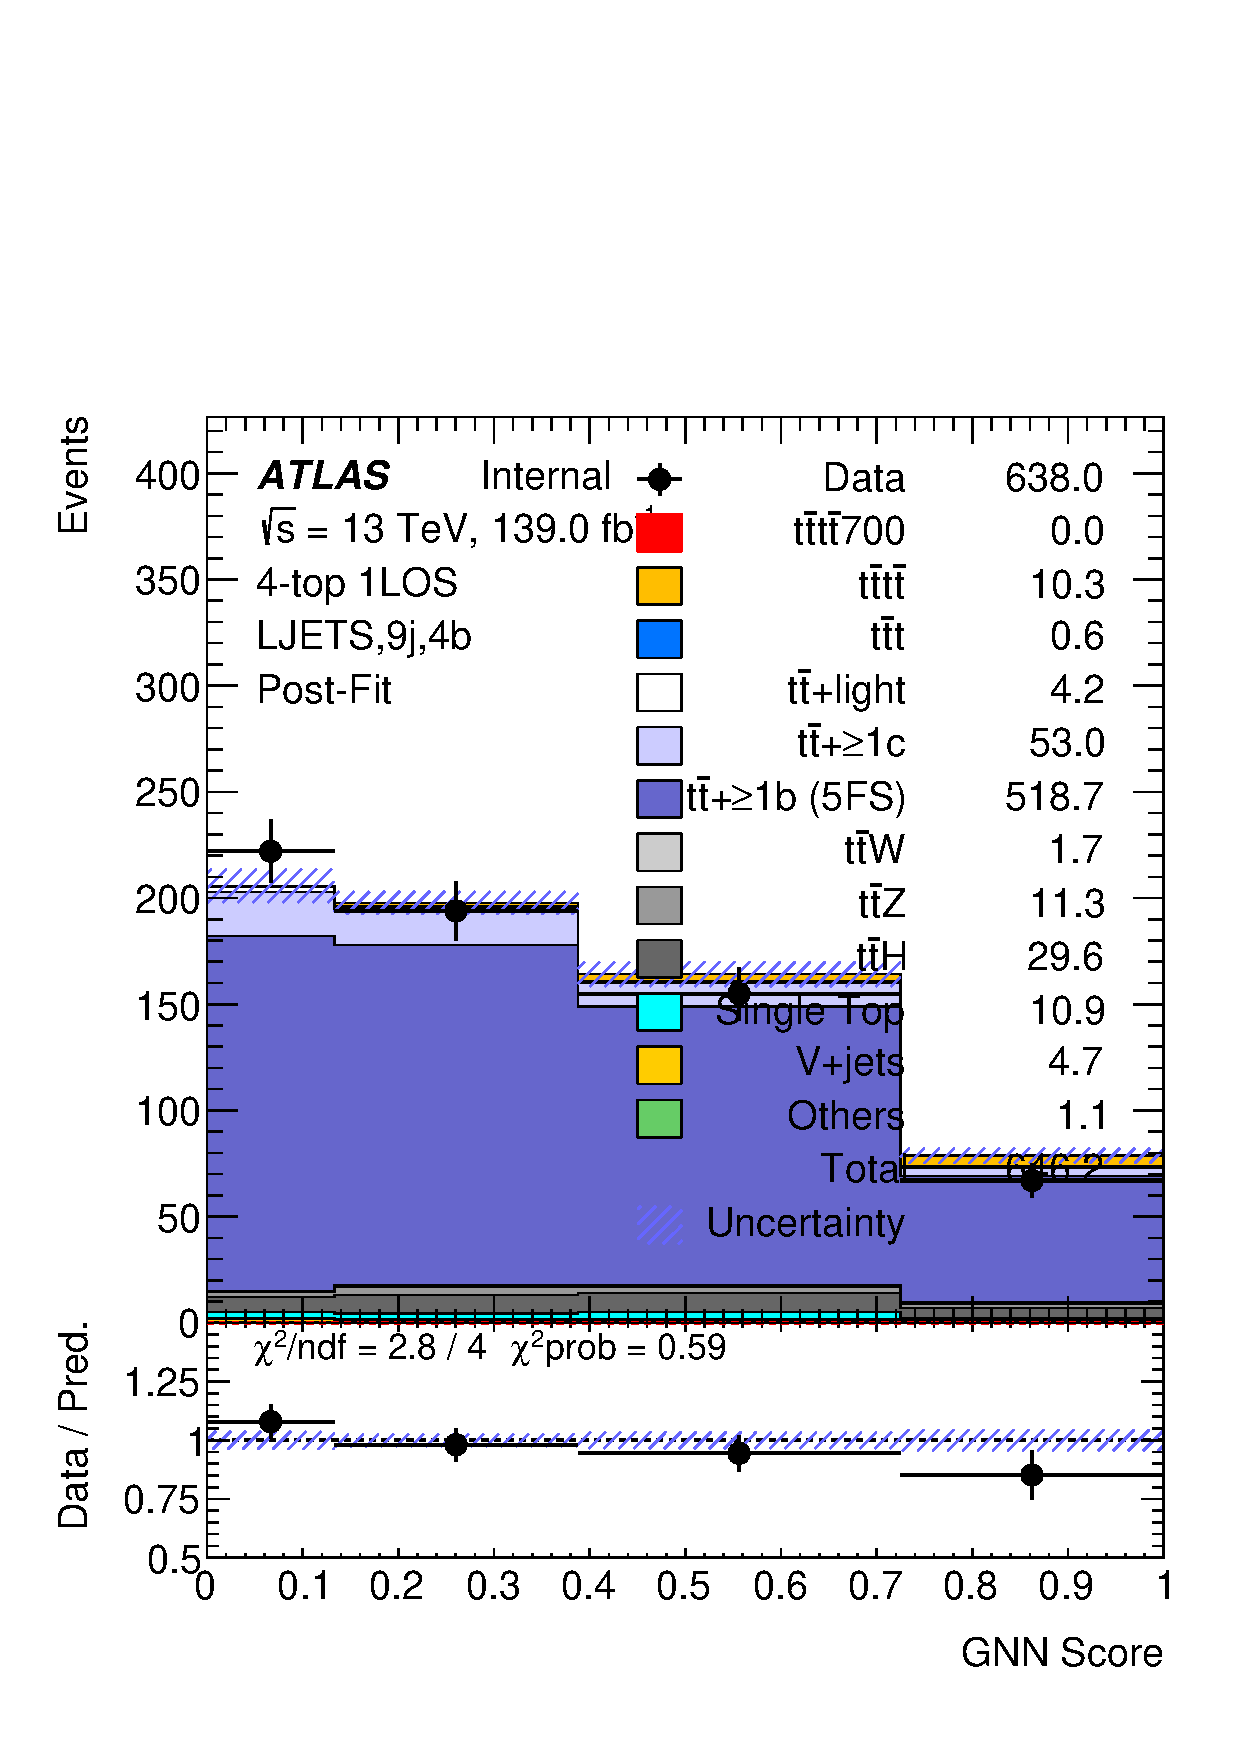
\includegraphics[width=0.23 \textwidth]{figures/fits/GNN/700/all/data_unblindedBonly/Plots/ljets_9j4b_postFit.pdf} &
        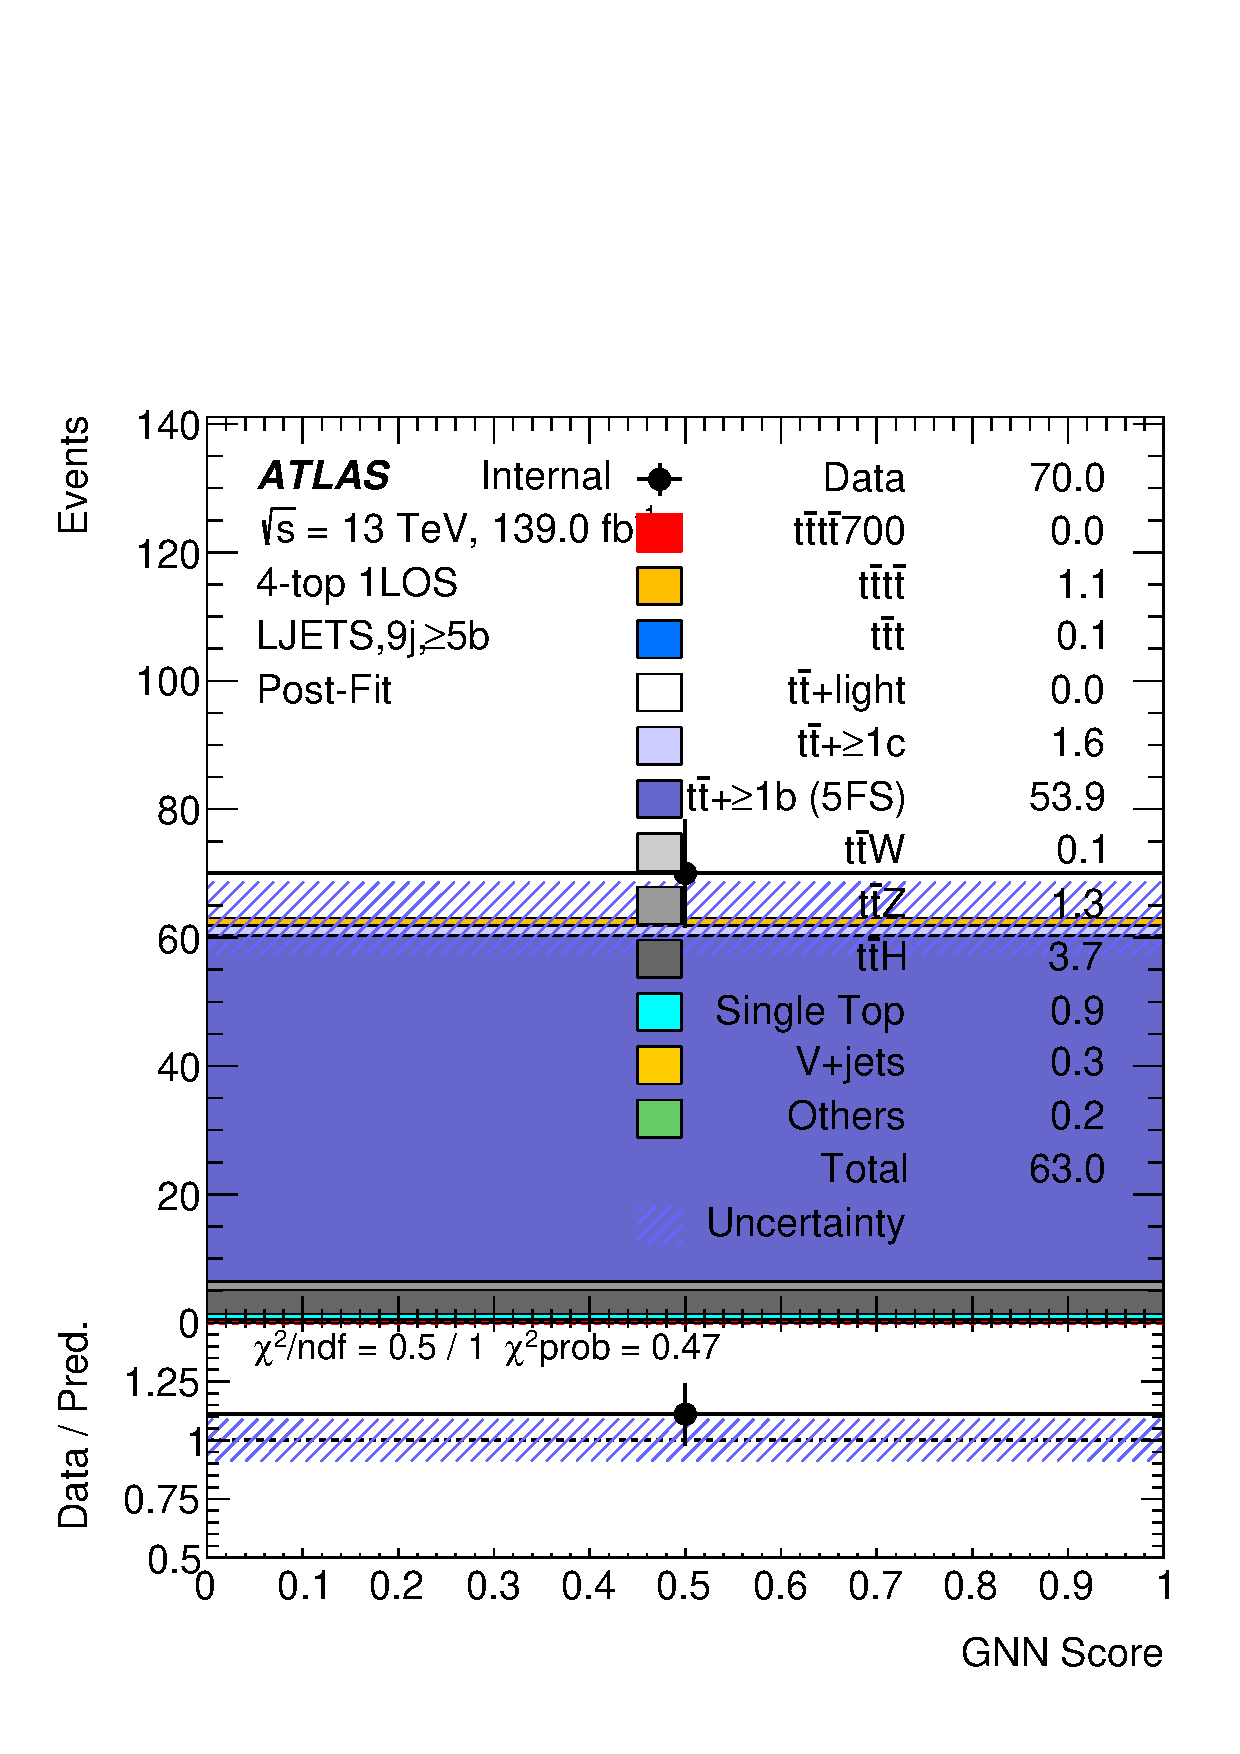
\includegraphics[width=0.23 \textwidth]{figures/fits/GNN/700/all/data_unblindedBonly/Plots/ljets_9jge5b_postFit.pdf} \\

        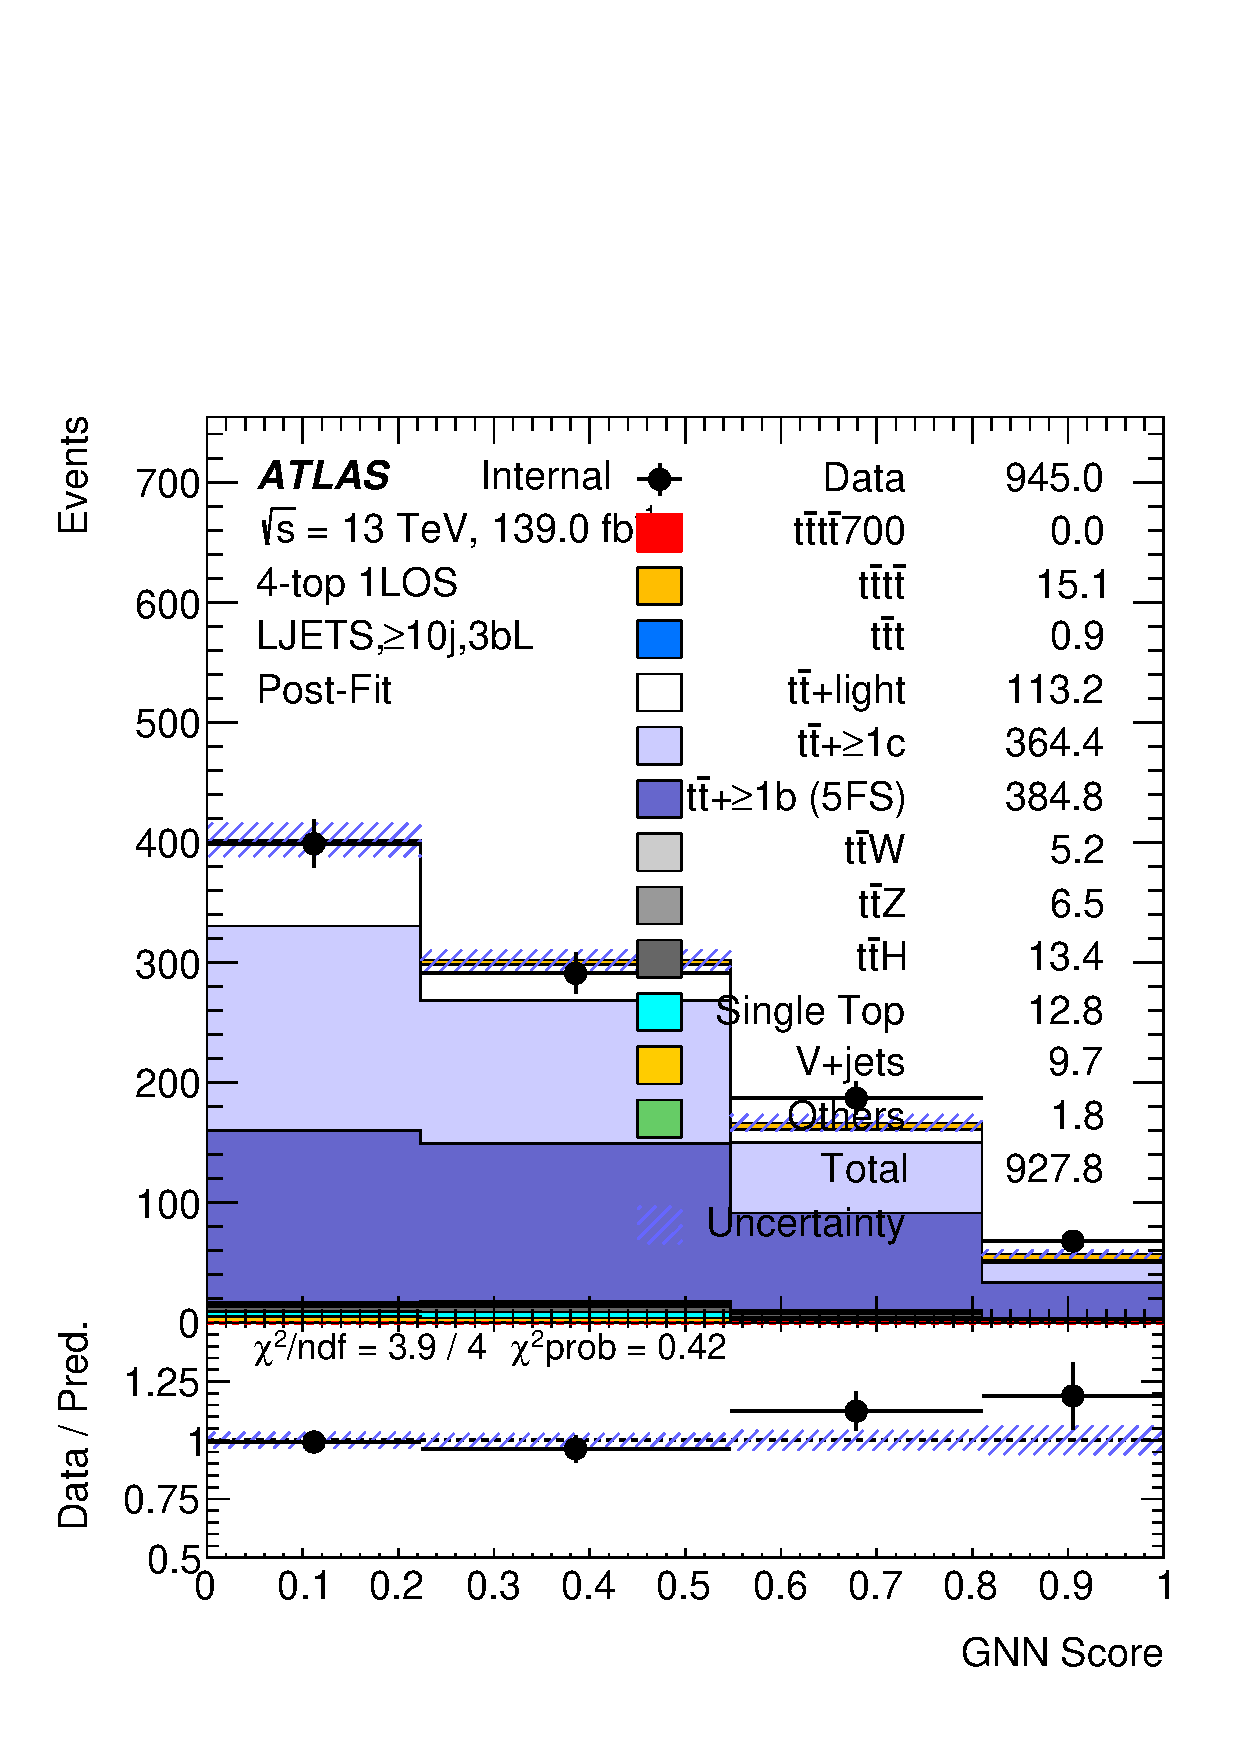
\includegraphics[width=0.23 \textwidth]{figures/fits/GNN/700/all/data_unblindedBonly/Plots/ljets_ge10j3bL_postFit.pdf} &
        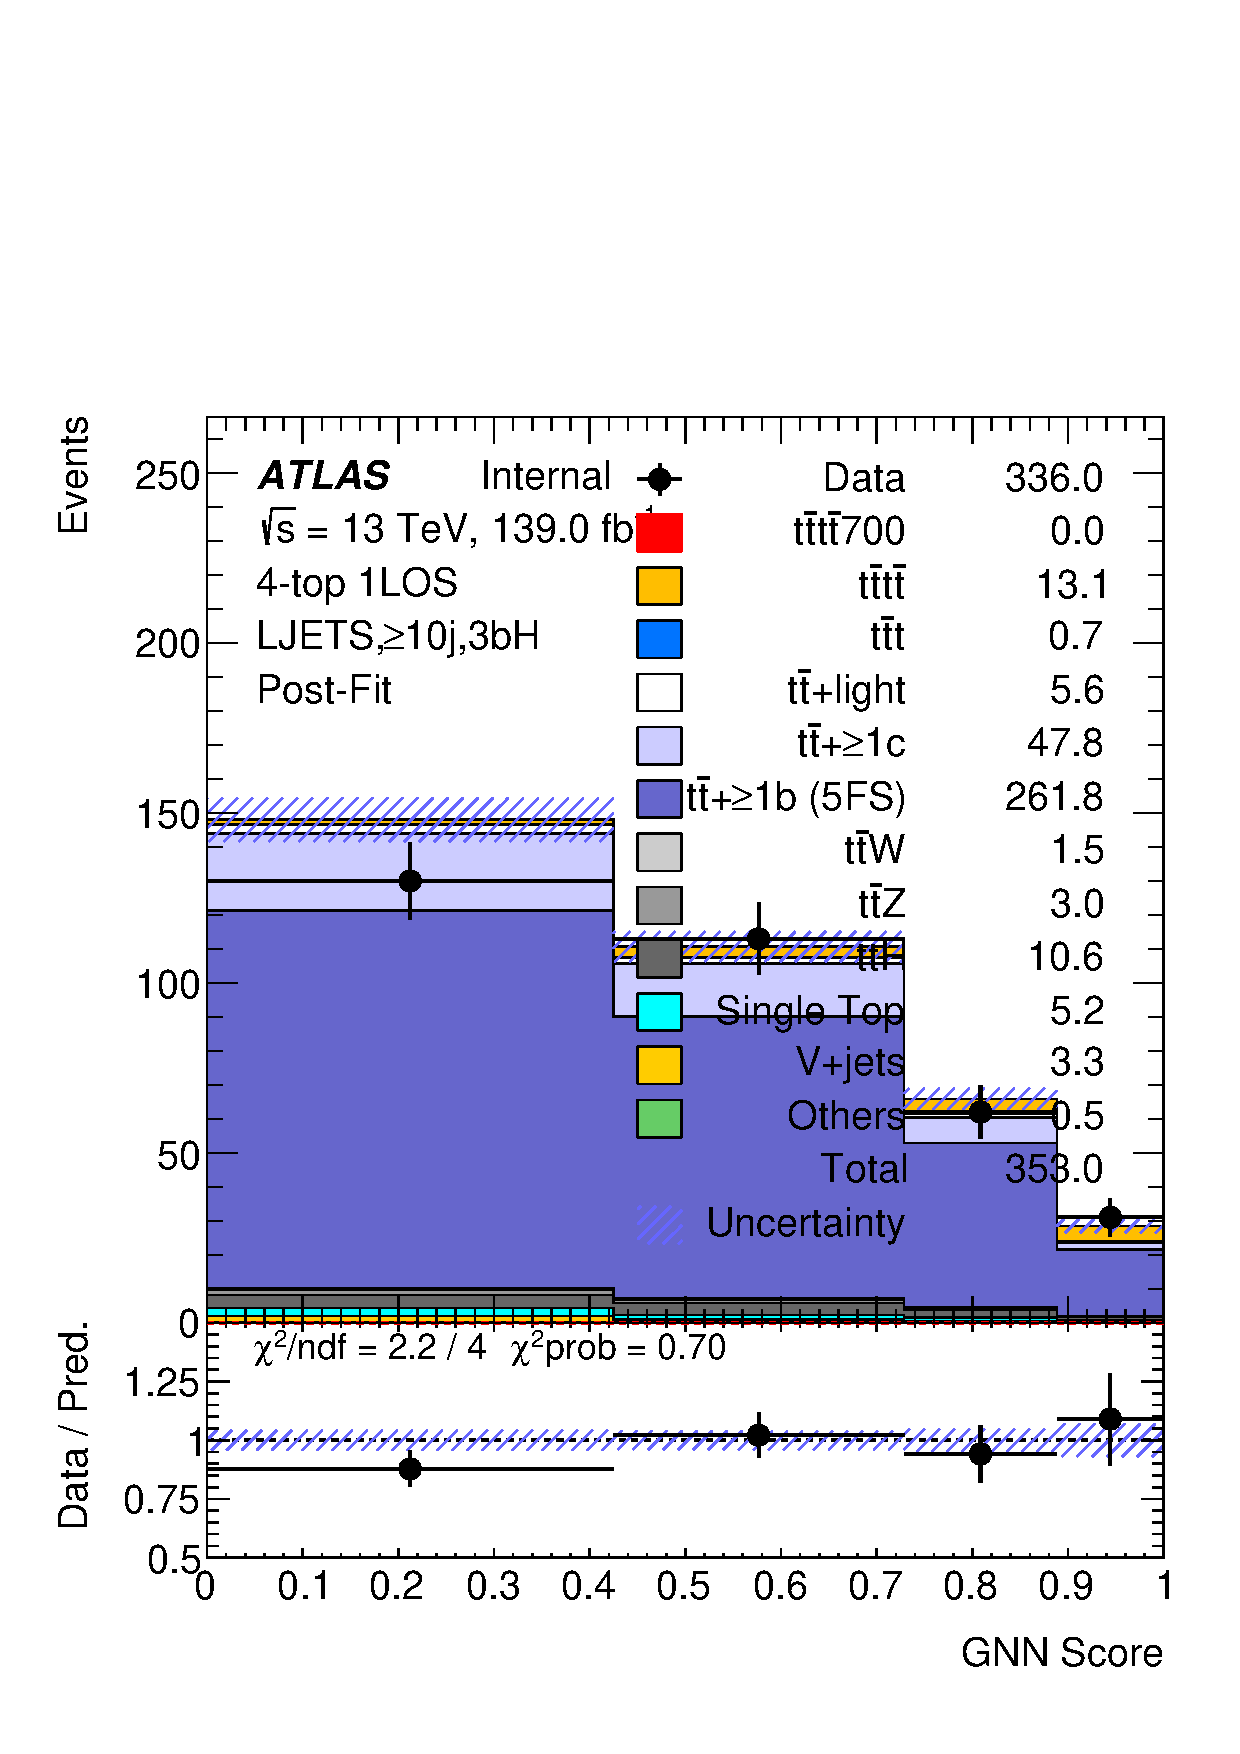
\includegraphics[width=0.23 \textwidth]{figures/fits/GNN/700/all/data_unblindedBonly/Plots/ljets_ge10j3bH_postFit.pdf} &
        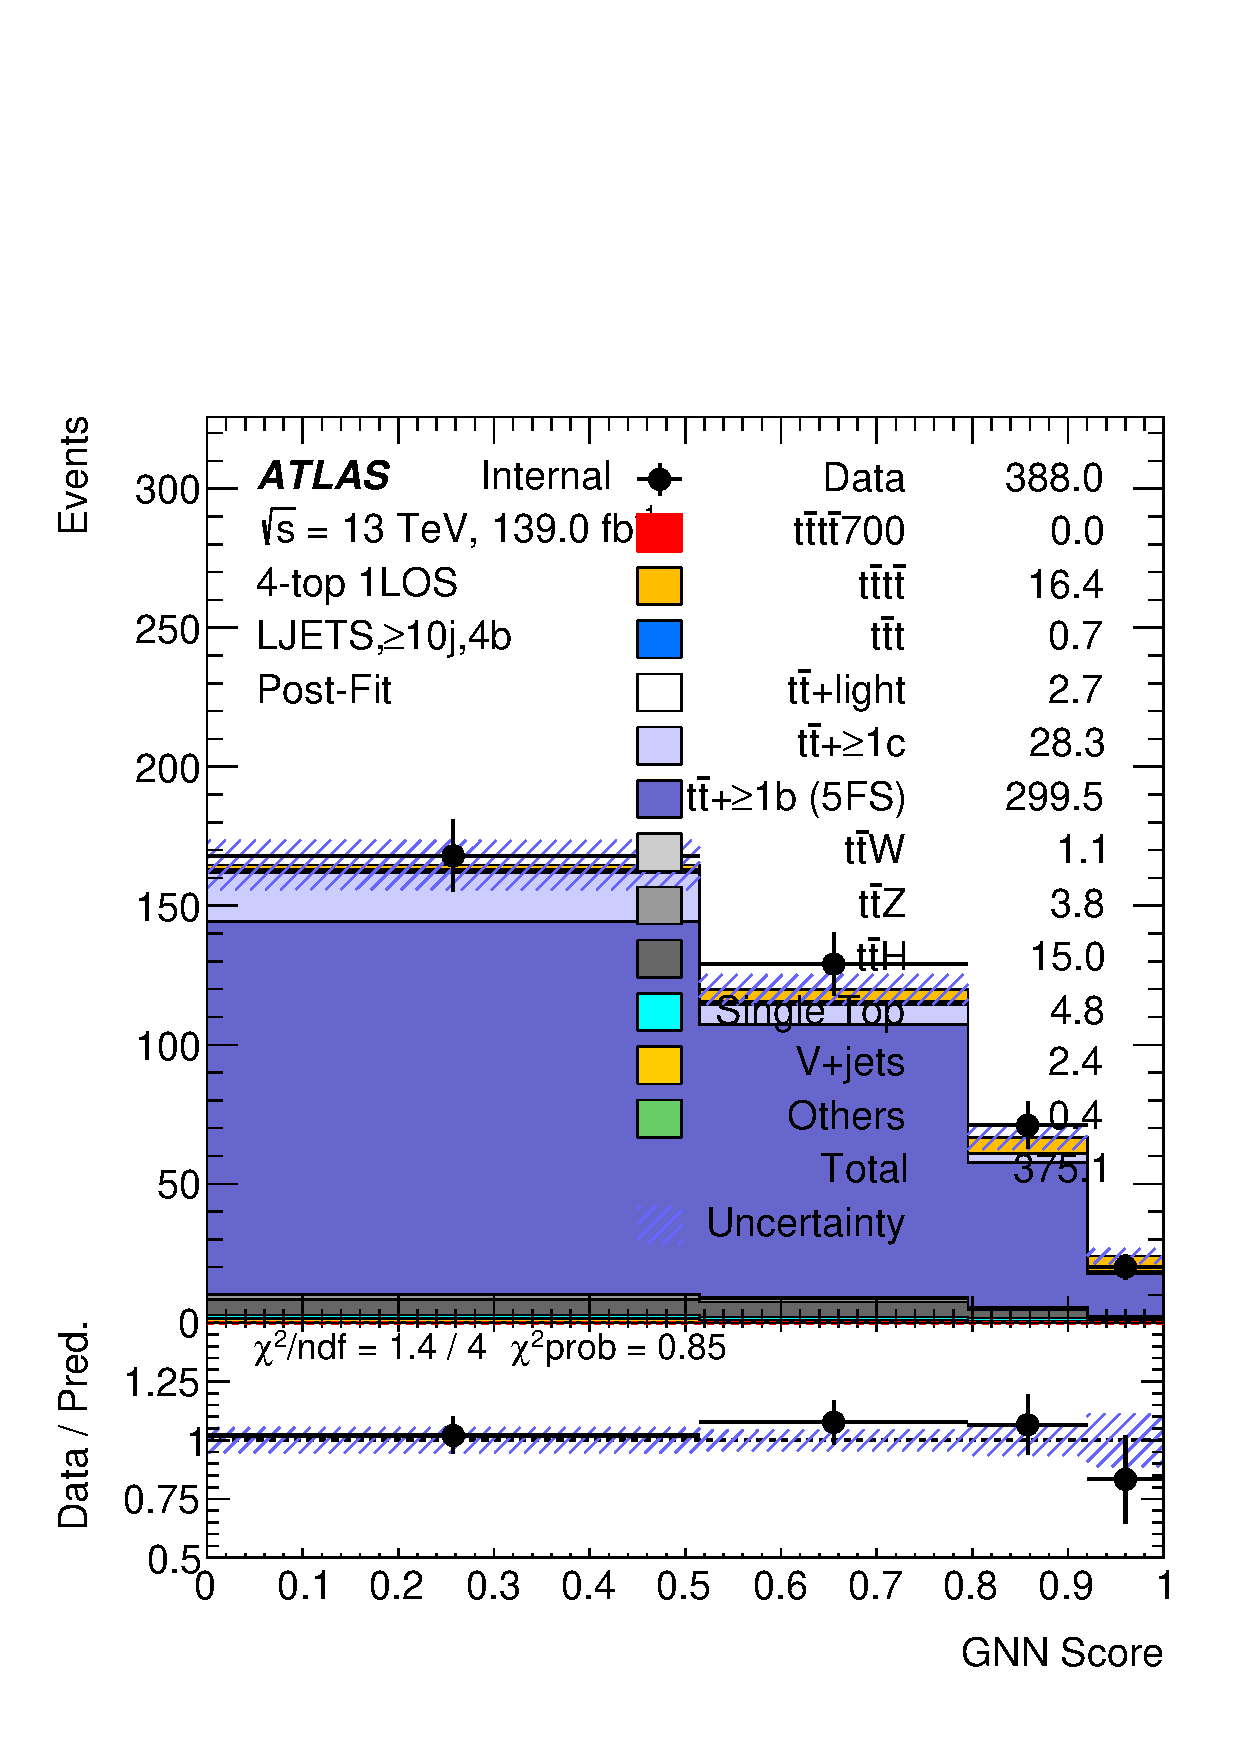
\includegraphics[width=0.23 \textwidth]{figures/fits/GNN/700/all/data_unblindedBonly/Plots/ljets_ge10j4b_postFit.pdf} &
        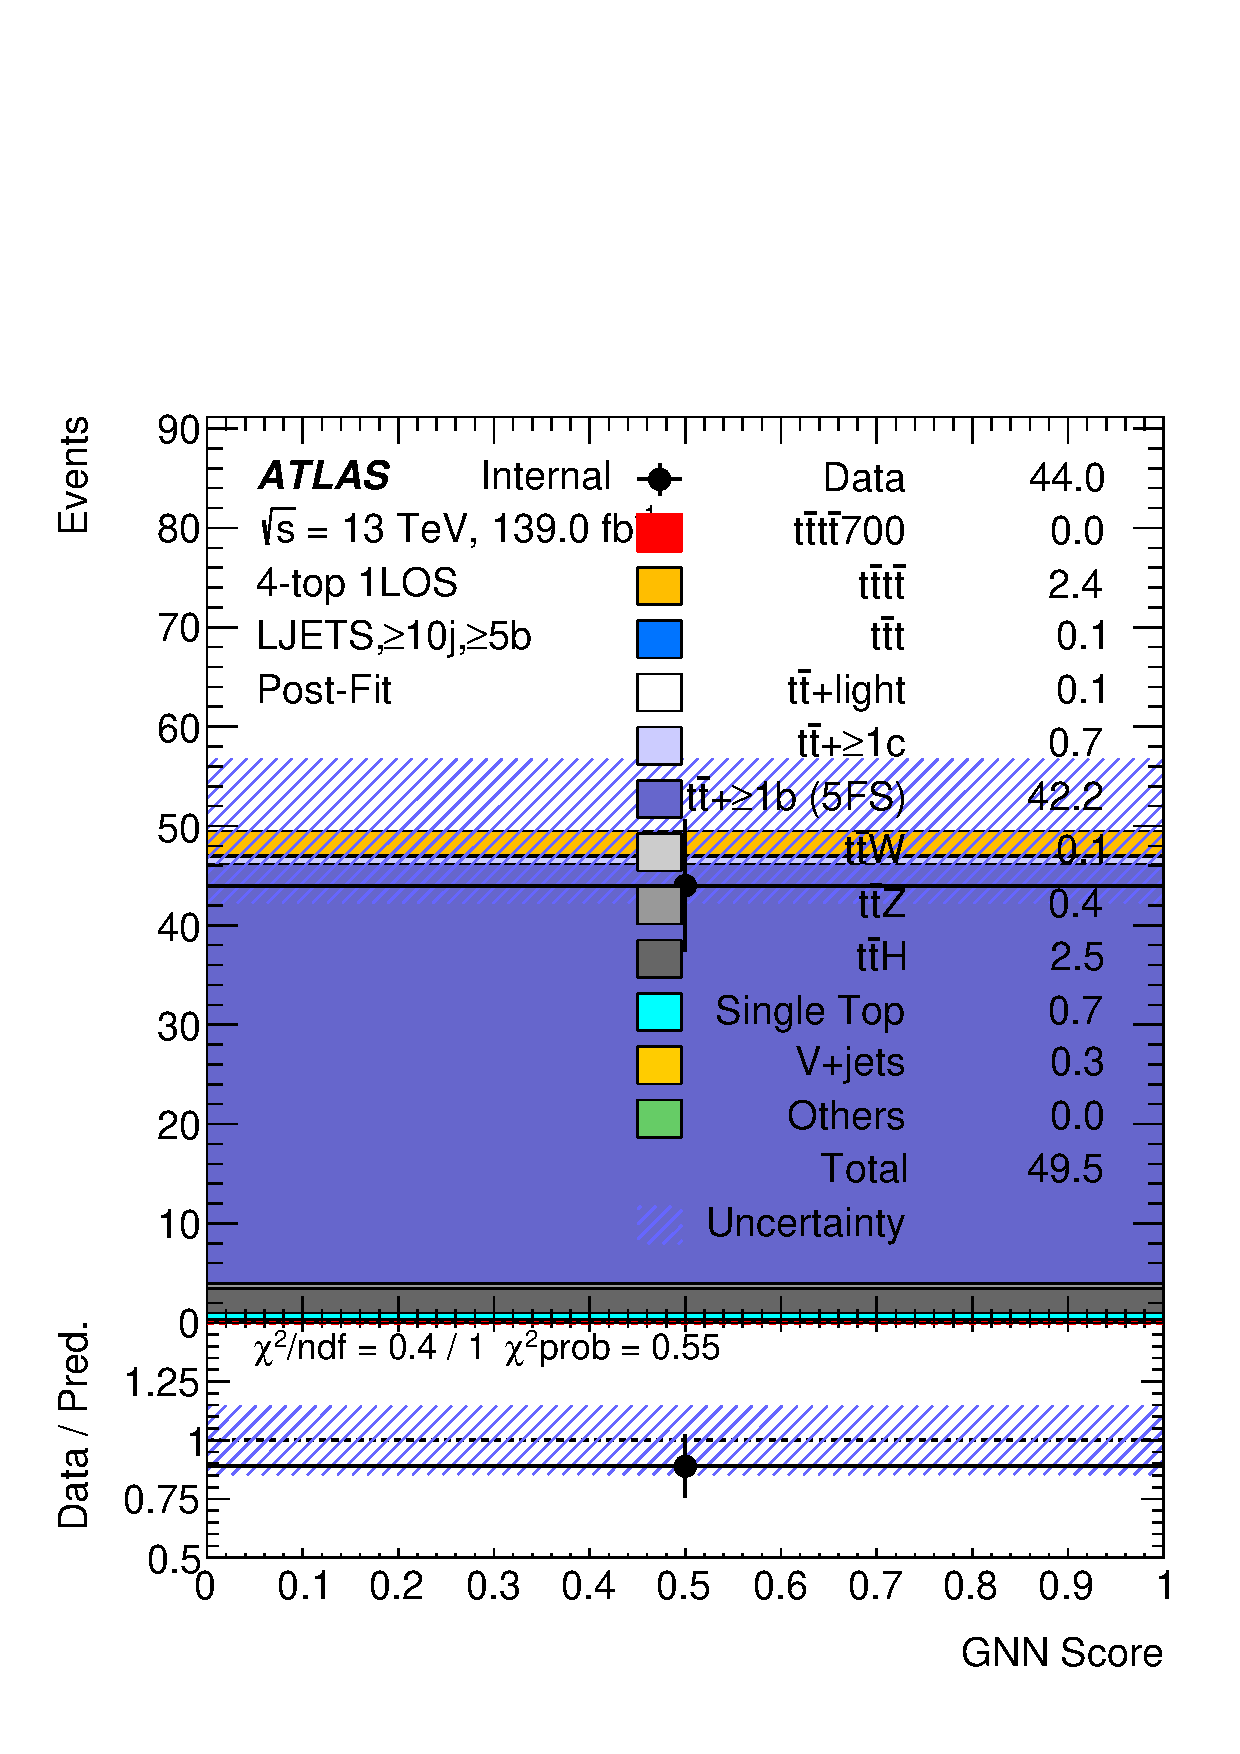
\includegraphics[width=0.23 \textwidth]{figures/fits/GNN/700/all/data_unblindedBonly/Plots/ljets_ge10jge5b_postFit.pdf} \\
        \end{tabular}
        \caption{\label{fig:Postfit_Yields_1L_700GeV}Post-fit distributions for 1L regions associated with different signal and background samples, compared with data yields for mH = 700 GeV. The fit is done using all regions (1L+2L). The same plots for mH = 400 GeV are shown in Figure \ref{fig:Postfit_Yields_1L}.}
\end{center}
\end{figure}

\begin{figure}[htbp!]
        \begin{center} \setlength{\tabcolsep}{2.5pt}\footnotesize
        \begin{tabular}{ccc}
        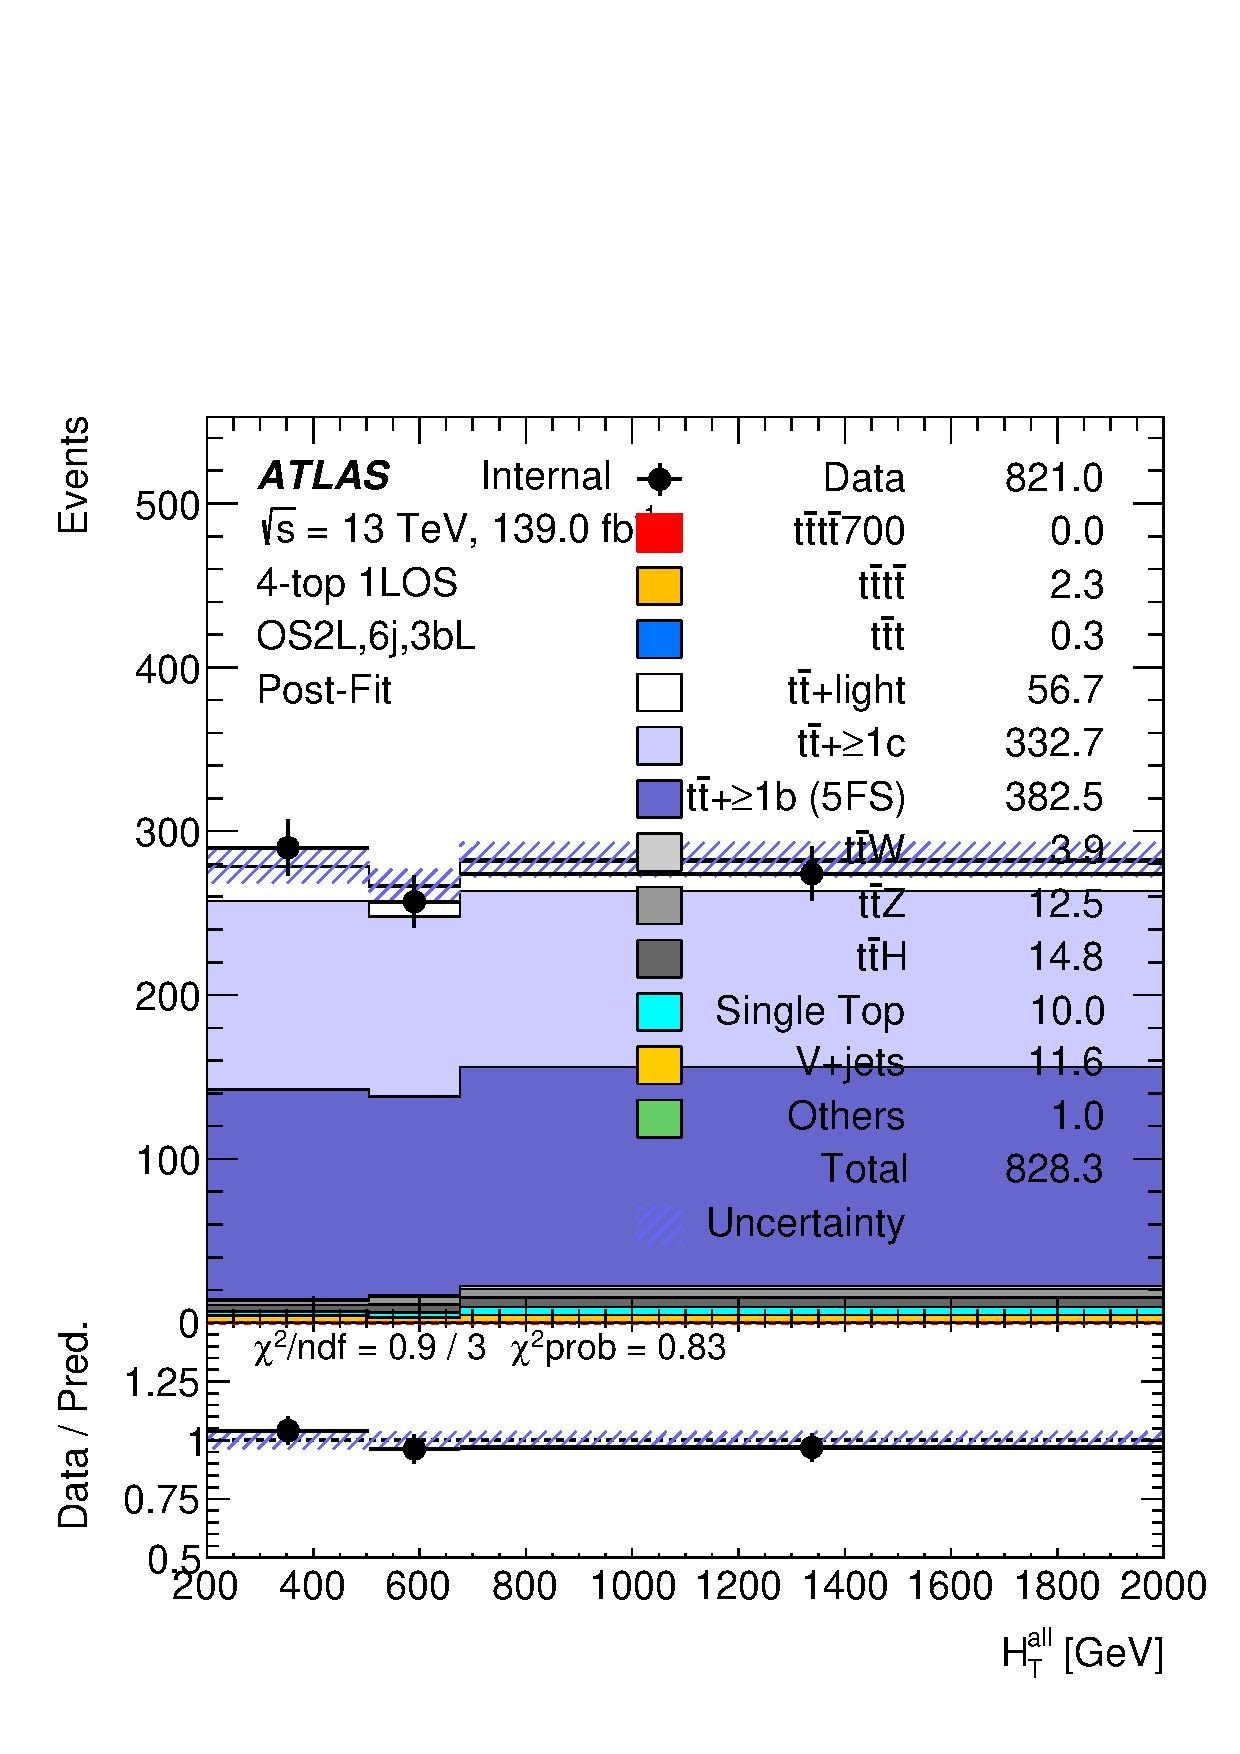
\includegraphics[width=0.31 \textwidth]{figures/fits/GNN/700/all/data_unblindedBonly/Plots/os2l_6j3bL_postFit.pdf} &
        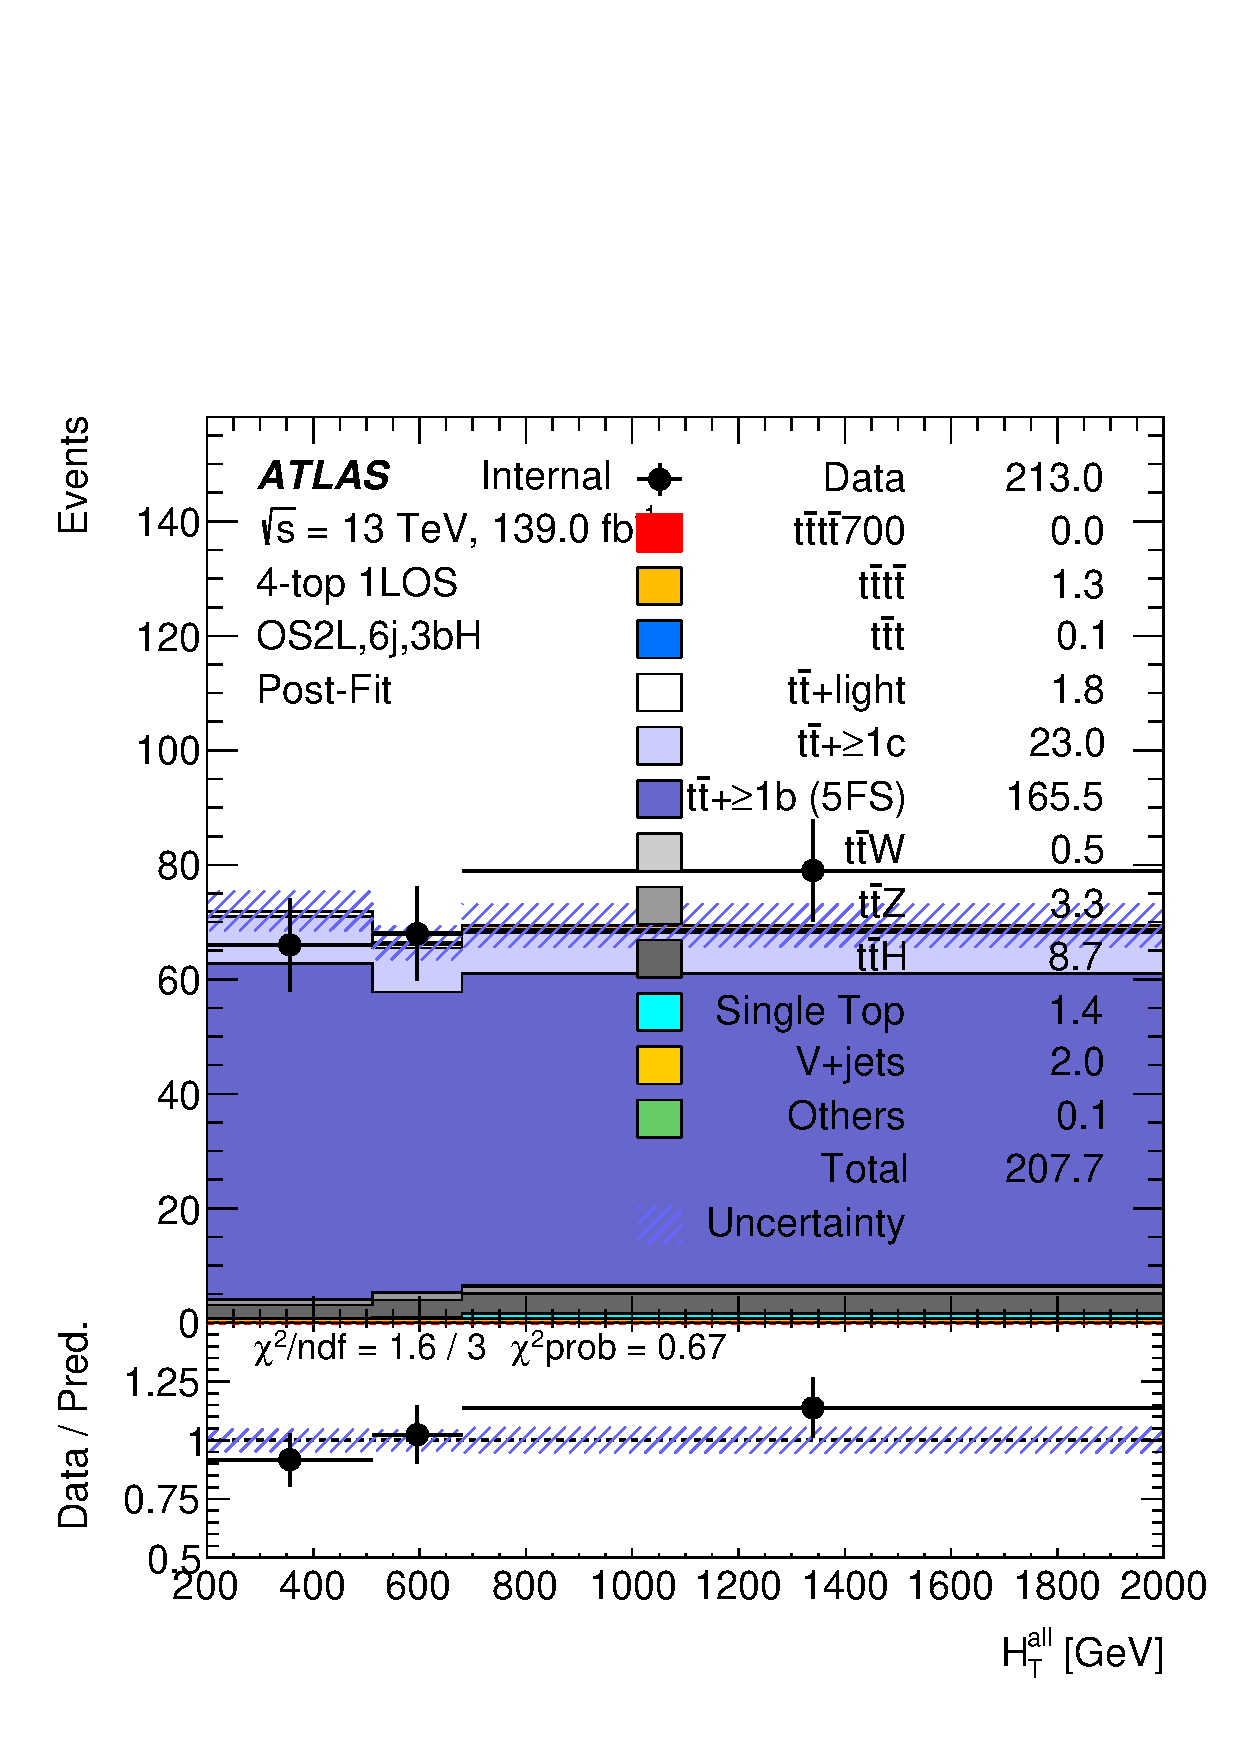
\includegraphics[width=0.31 \textwidth]{figures/fits/GNN/700/all/data_unblindedBonly/Plots/os2l_6j3bH_postFit.pdf} &
        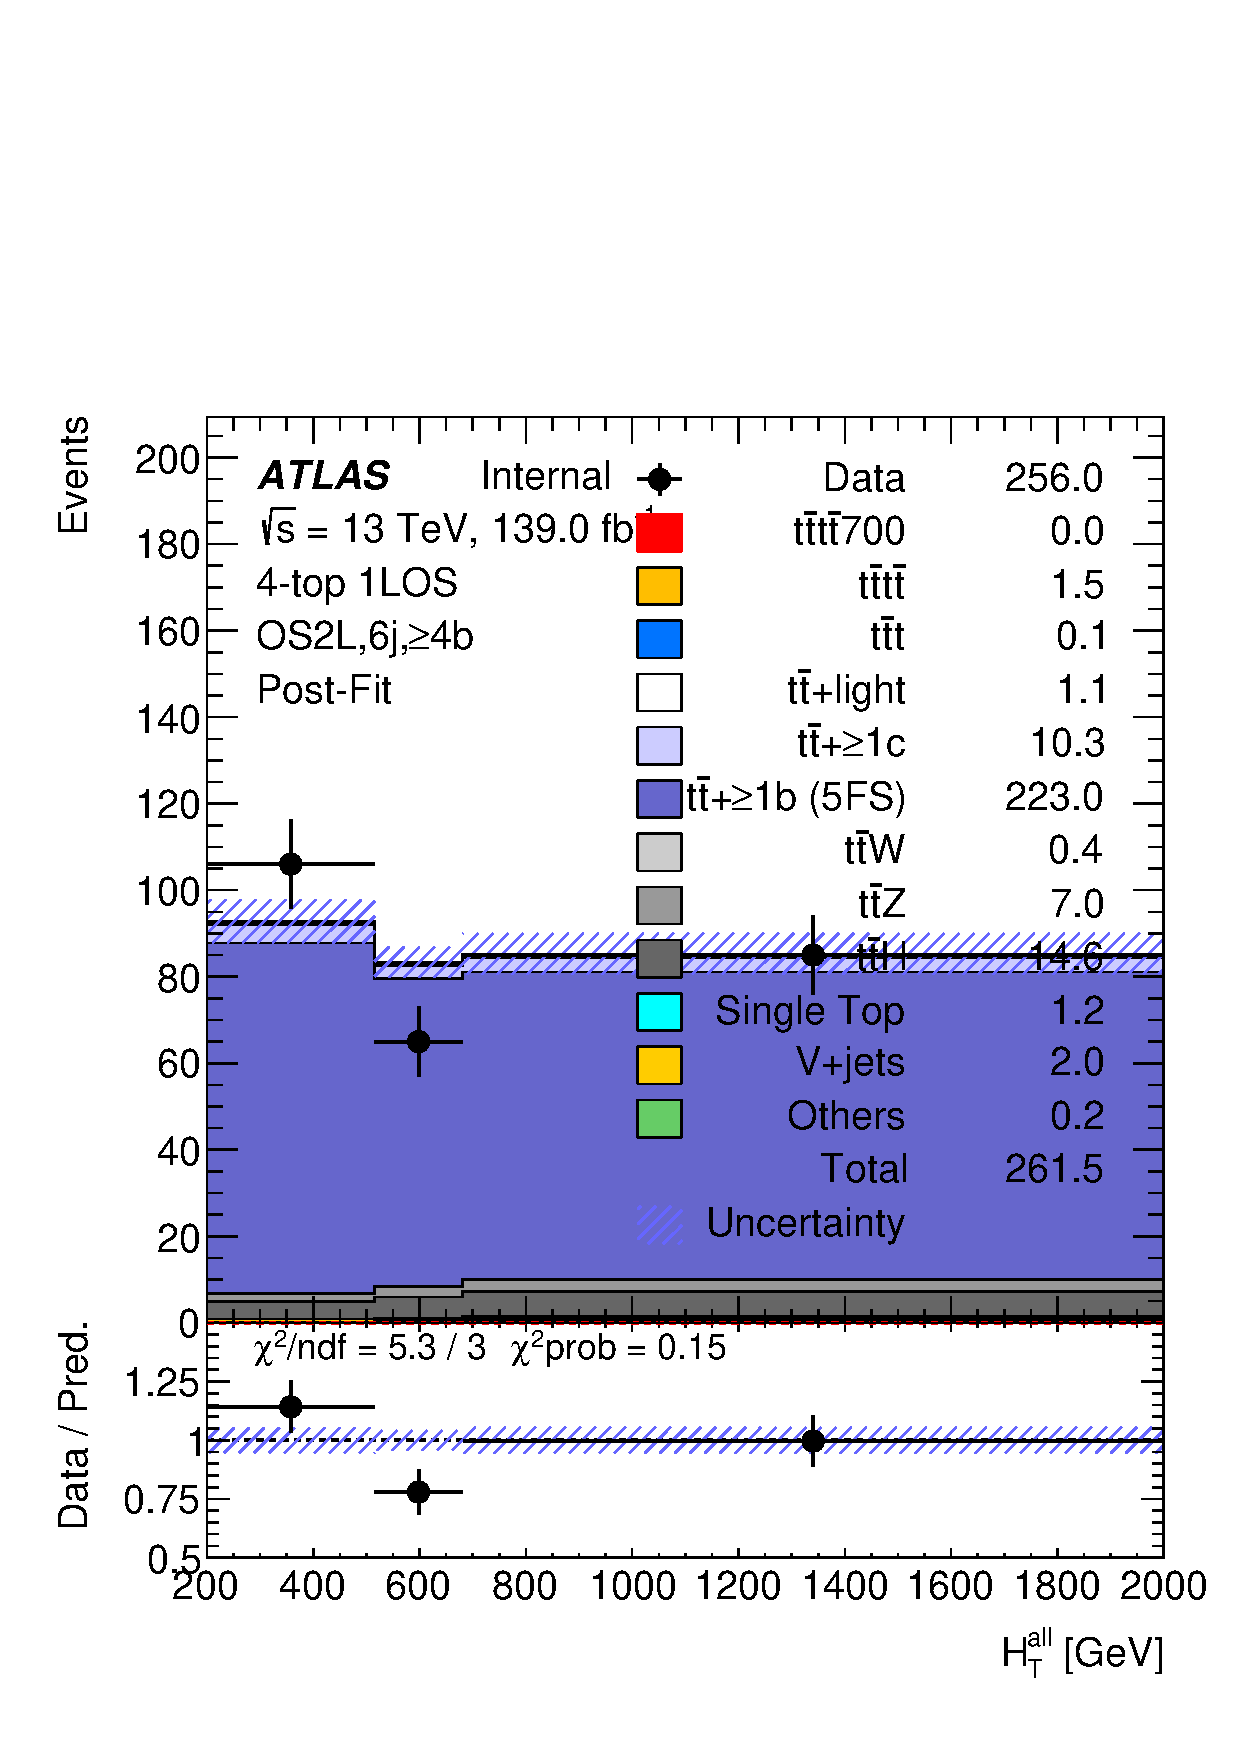
\includegraphics[width=0.31 \textwidth]{figures/fits/GNN/700/all/data_unblindedBonly/Plots/os2l_6jge4b_postFit.pdf} \\

        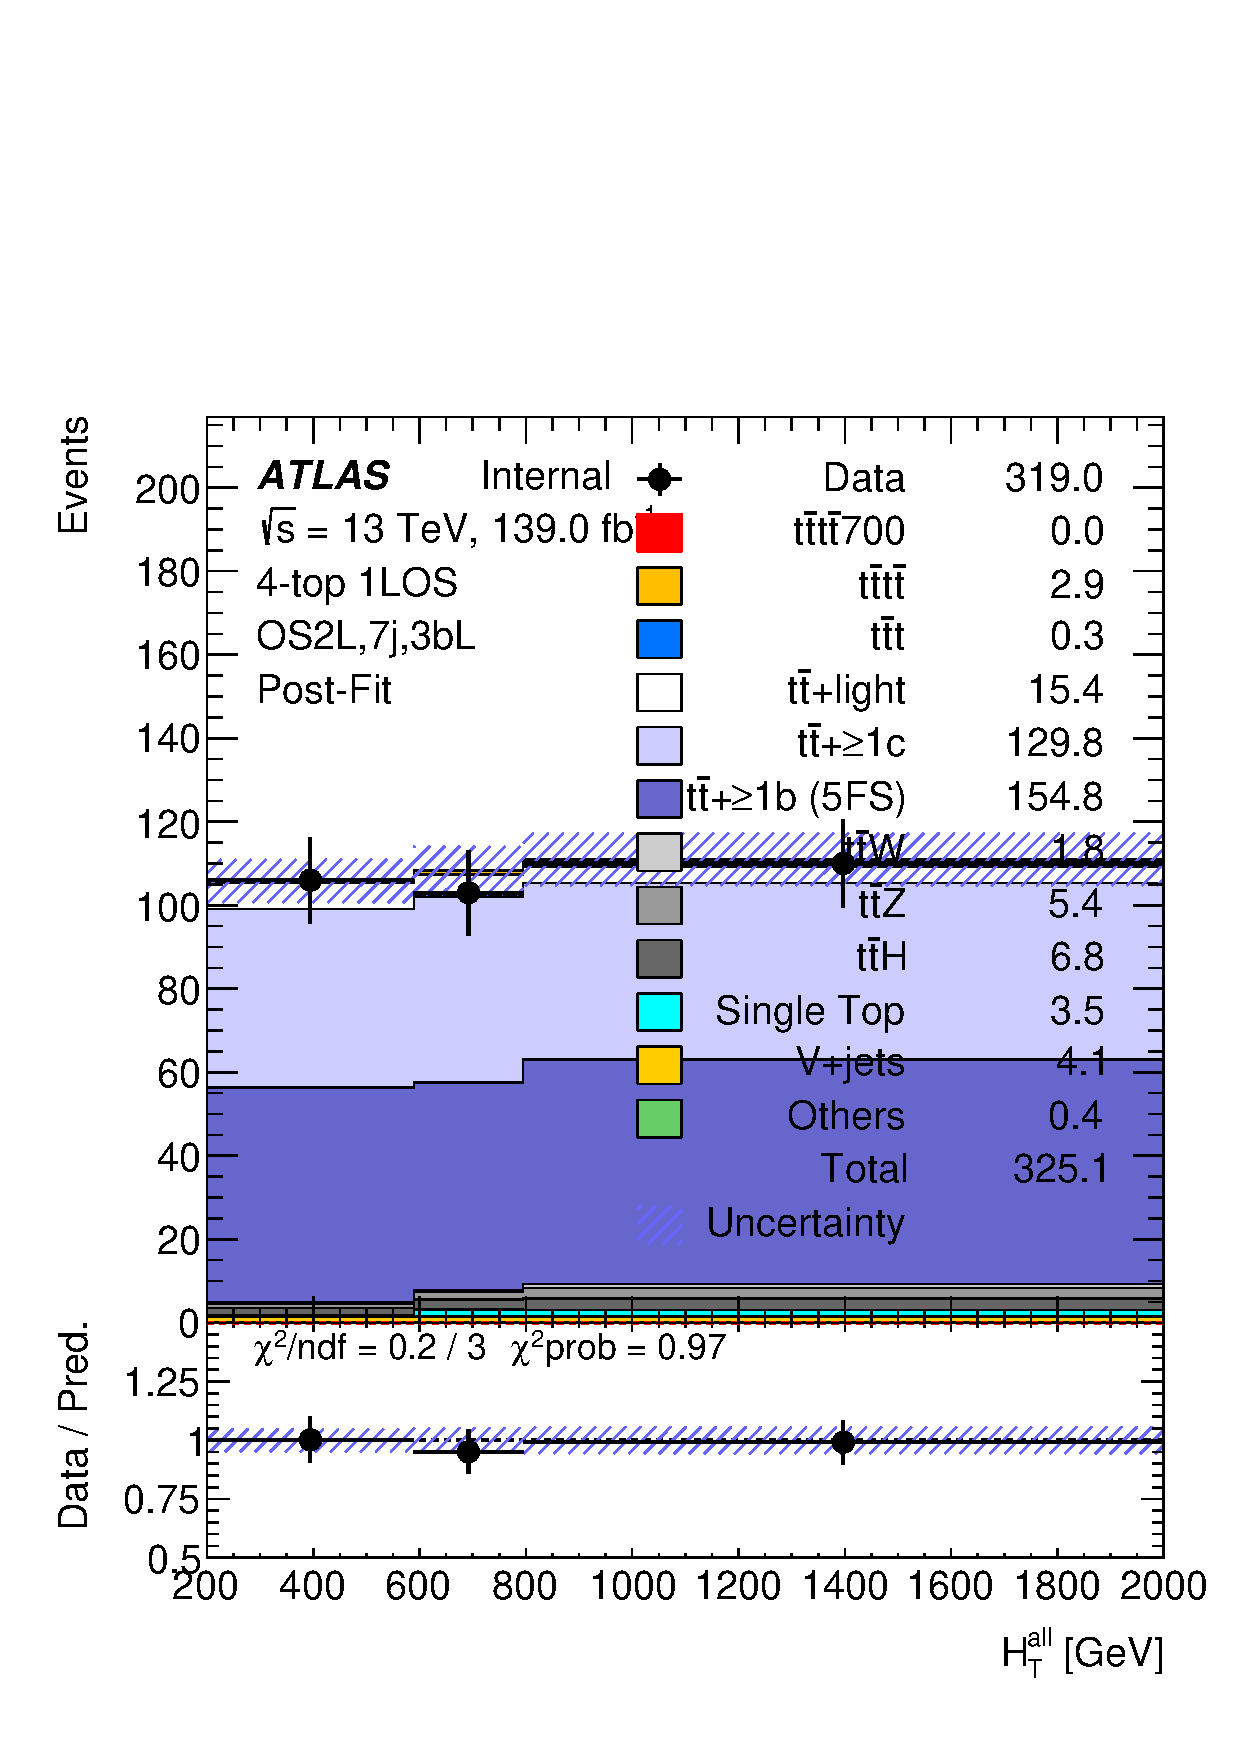
\includegraphics[width=0.31 \textwidth]{figures/fits/GNN/700/all/data_unblindedBonly/Plots/os2l_7j3bL_postFit.pdf} &
        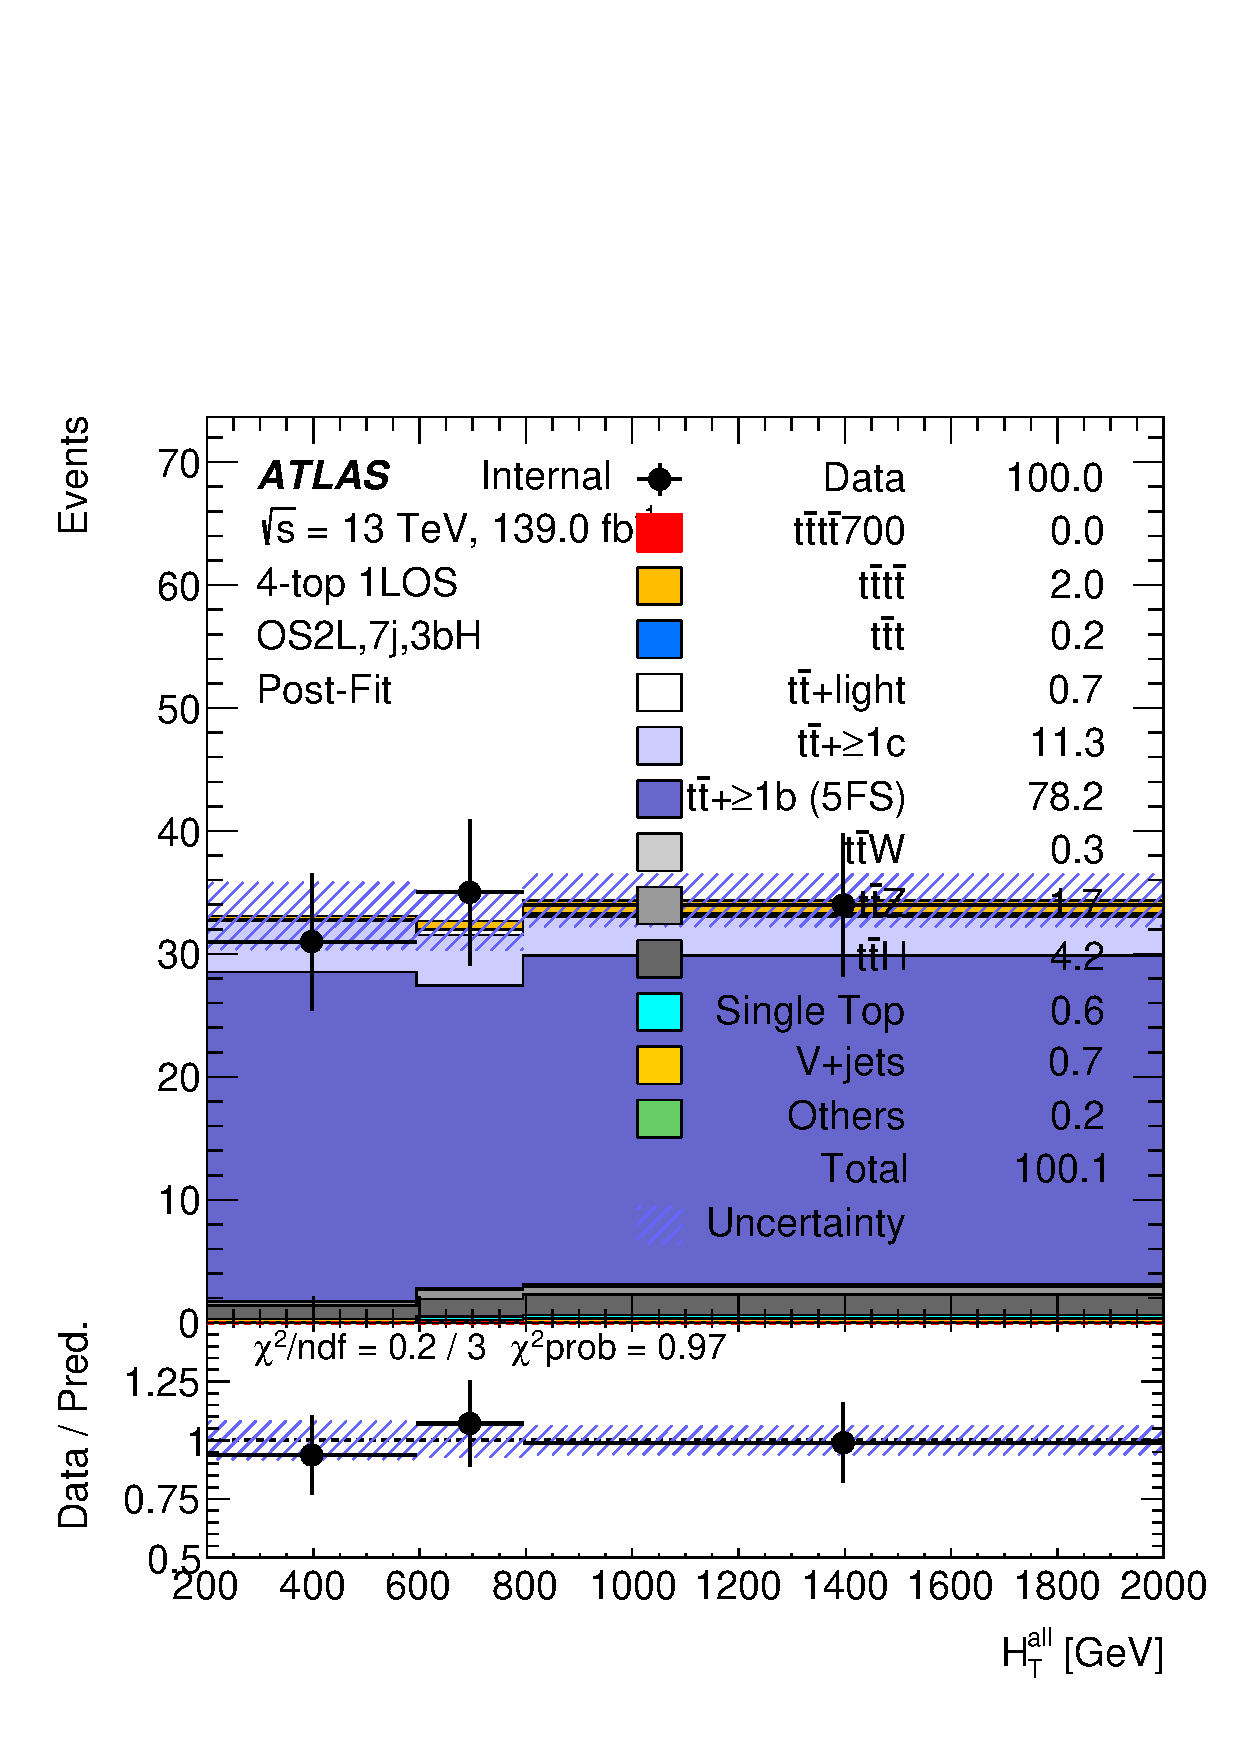
\includegraphics[width=0.31 \textwidth]{figures/fits/GNN/700/all/data_unblindedBonly/Plots/os2l_7j3bH_postFit.pdf} &
        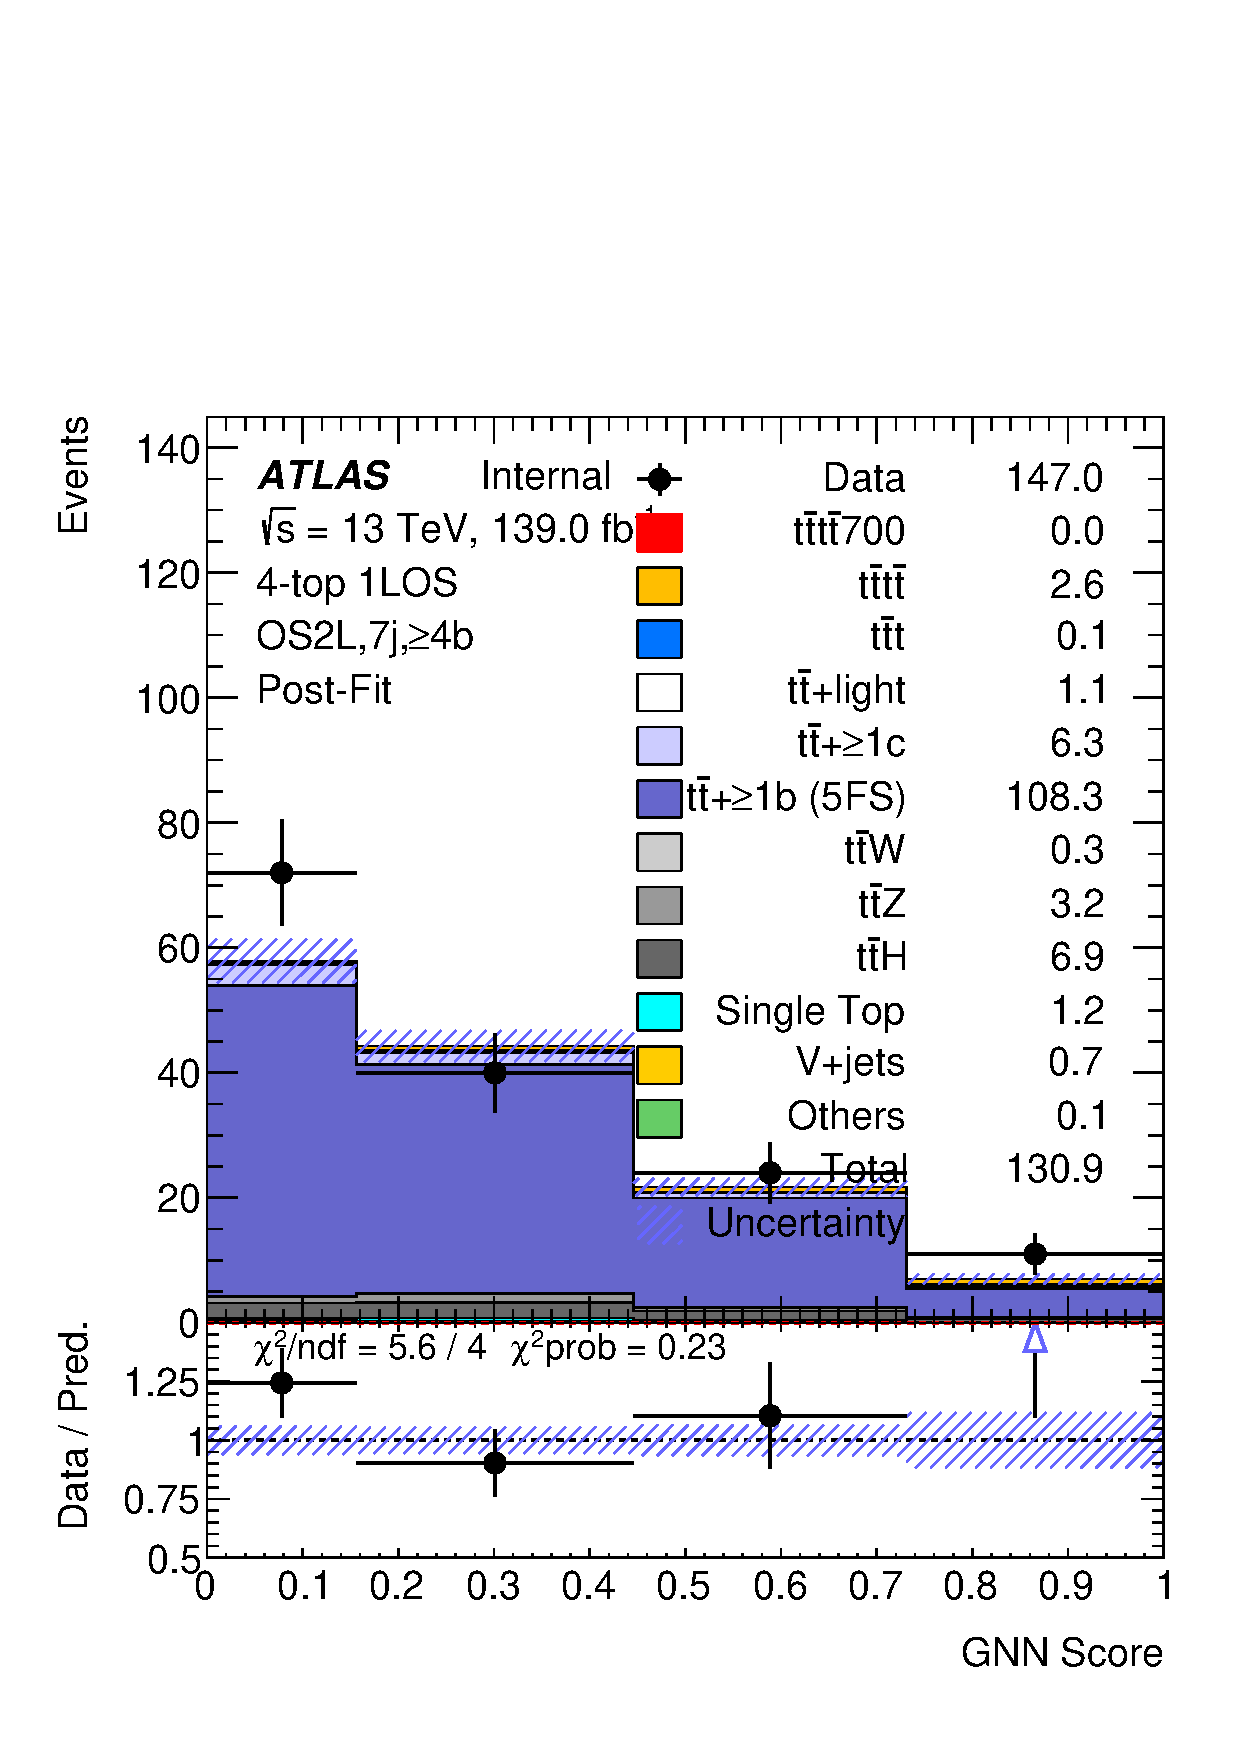
\includegraphics[width=0.31 \textwidth]{figures/fits/GNN/700/all/data_unblindedBonly/Plots/os2l_7jge4b_postFit.pdf} \\

        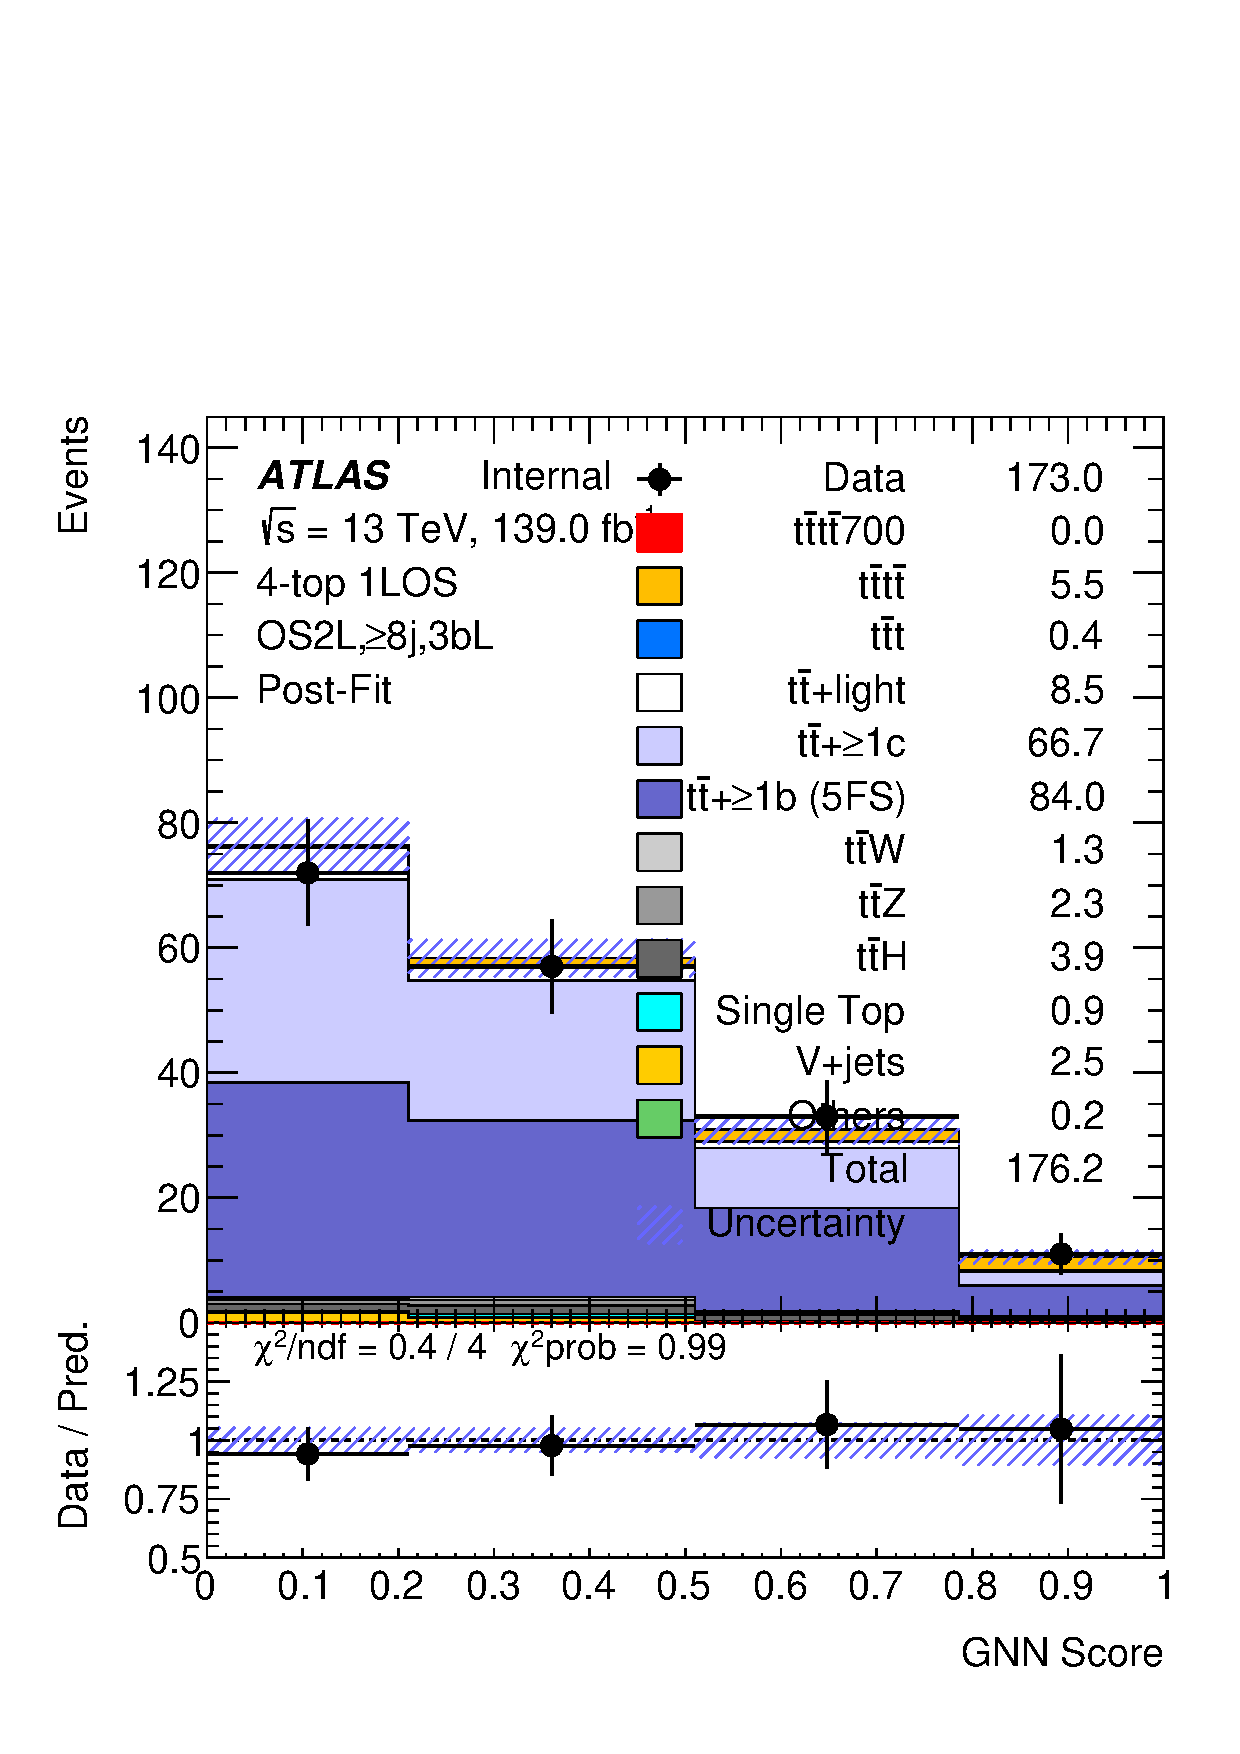
\includegraphics[width=0.31 \textwidth]{figures/fits/GNN/700/all/data_unblindedBonly/Plots/os2l_ge8j3bL_postFit.pdf} &
        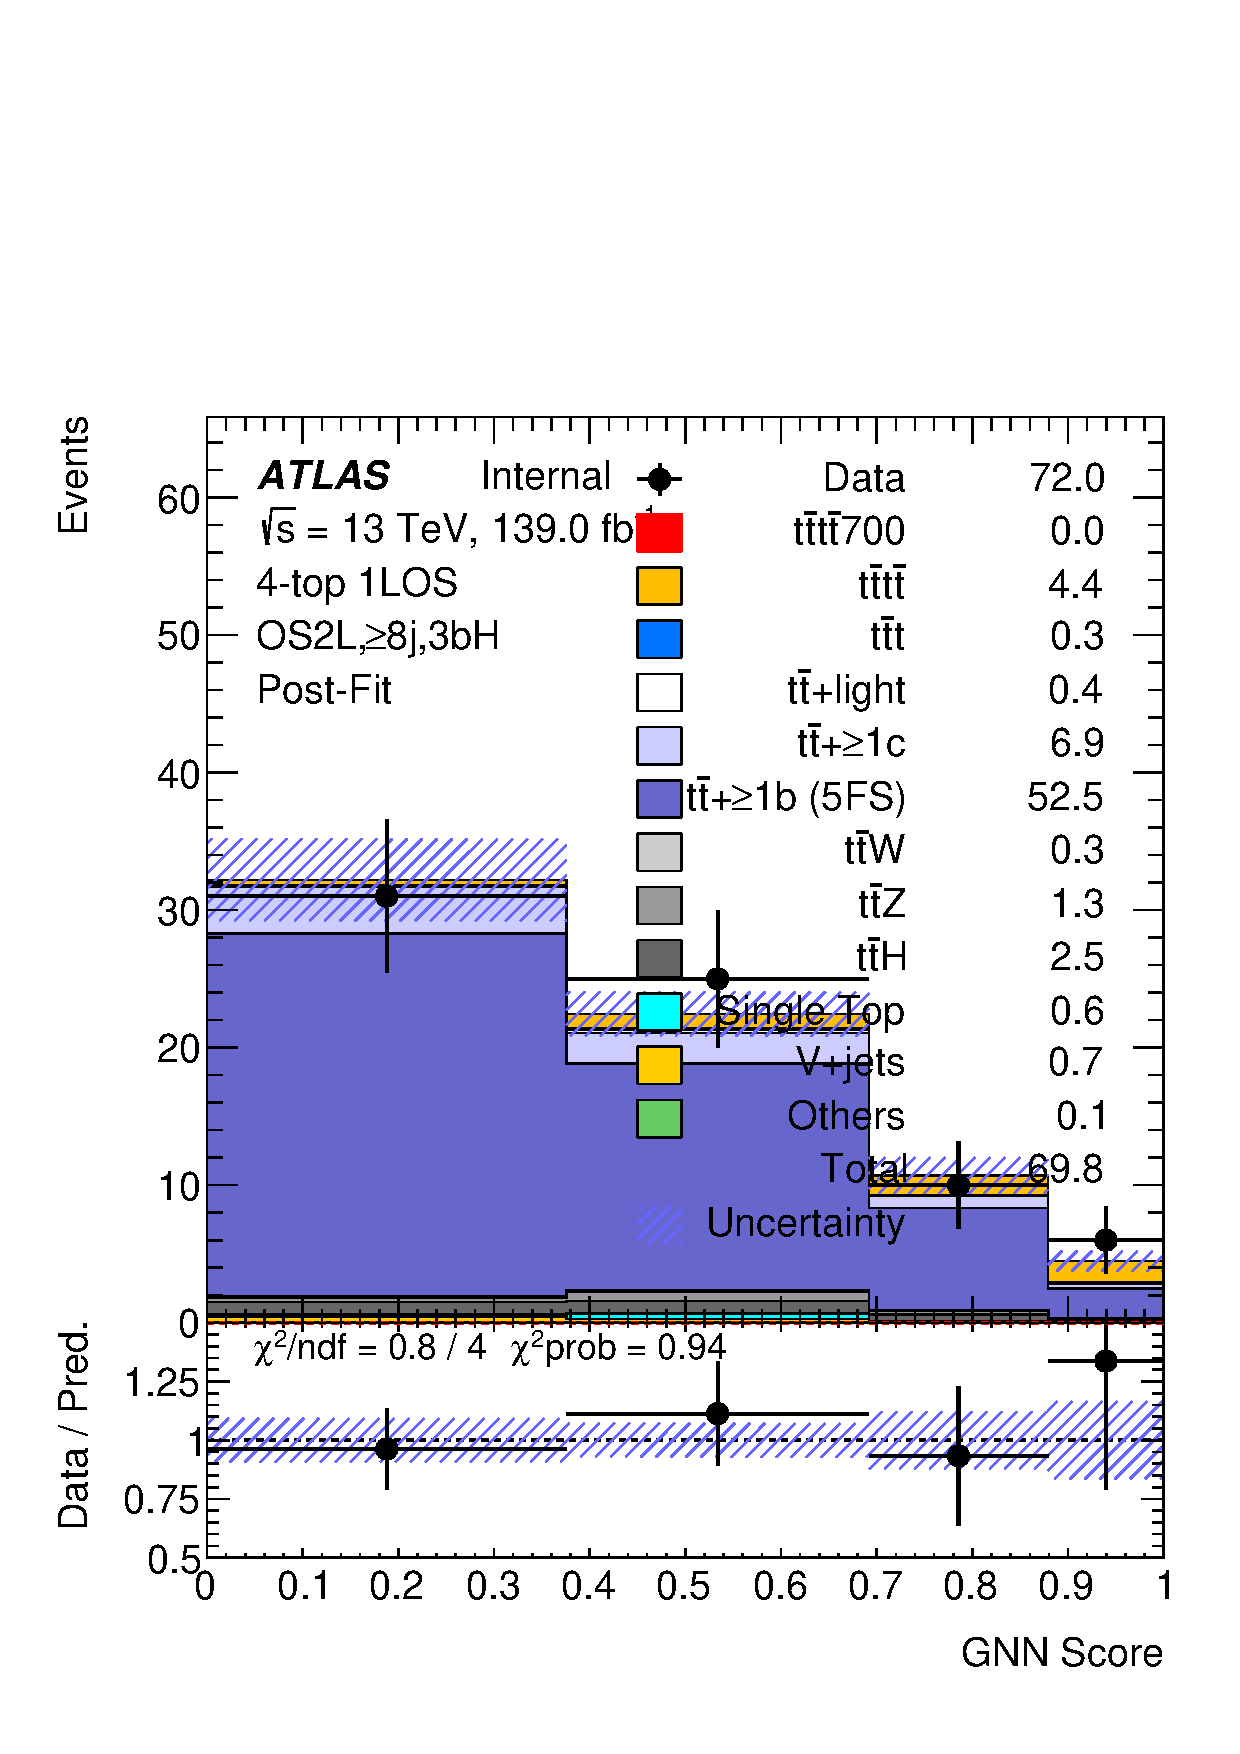
\includegraphics[width=0.31 \textwidth]{figures/fits/GNN/700/all/data_unblindedBonly/Plots/os2l_ge8j3bH_postFit.pdf} &
        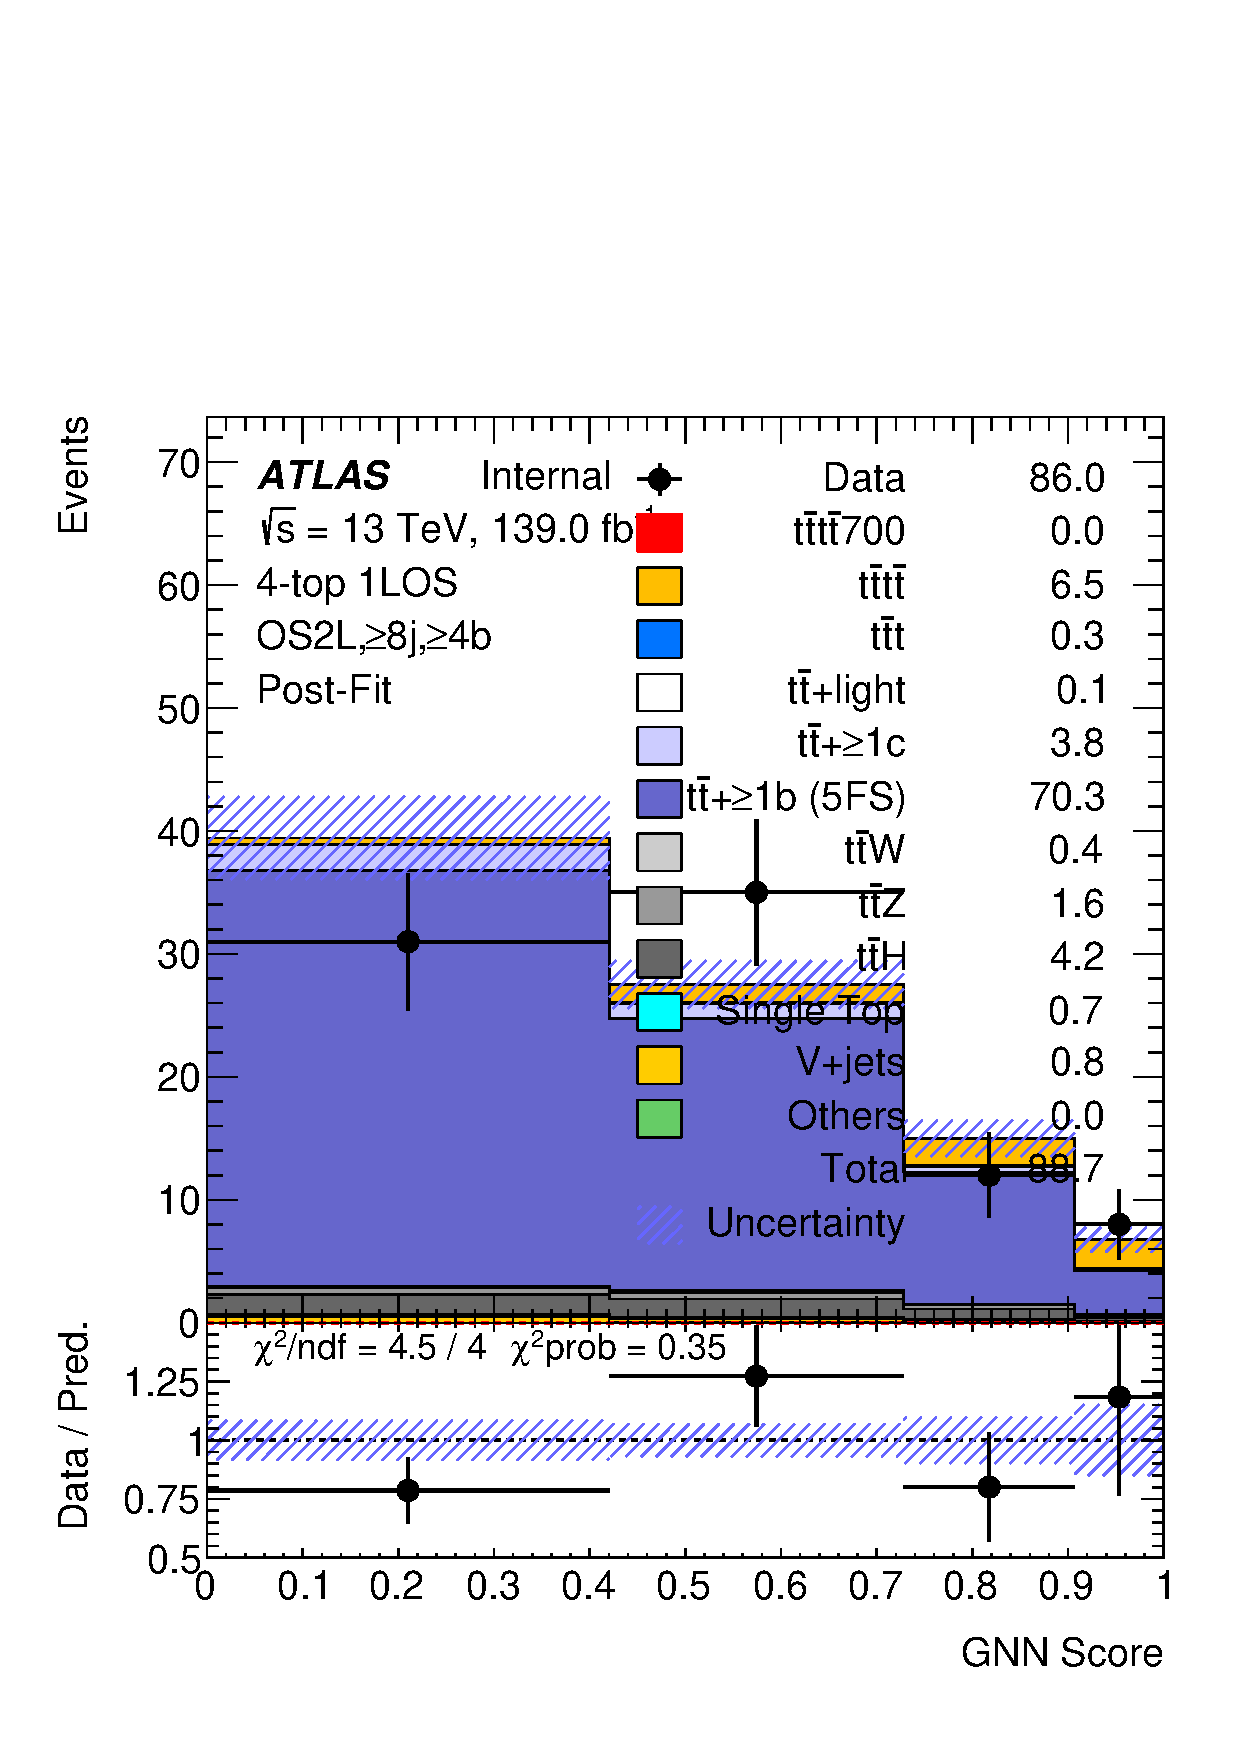
\includegraphics[width=0.31 \textwidth]{figures/fits/GNN/700/all/data_unblindedBonly/Plots/os2l_ge8jge4b_postFit.pdf} \\
        \end{tabular}
        \caption{\label{fig:Postfit_Yields_2L_700GeV}Post-fit distributions for 2LOS regions associated with different signal and background samples, compared with data yields for mH = 700 GeV. The fit is done using all regions (1L+2L). The same plots for mH = 400 GeV are shown in Figure \ref{fig:Postfit_Yields_2L}.}
\end{center}
\end{figure}

\begin{figure}[htbp!]
        \centering
        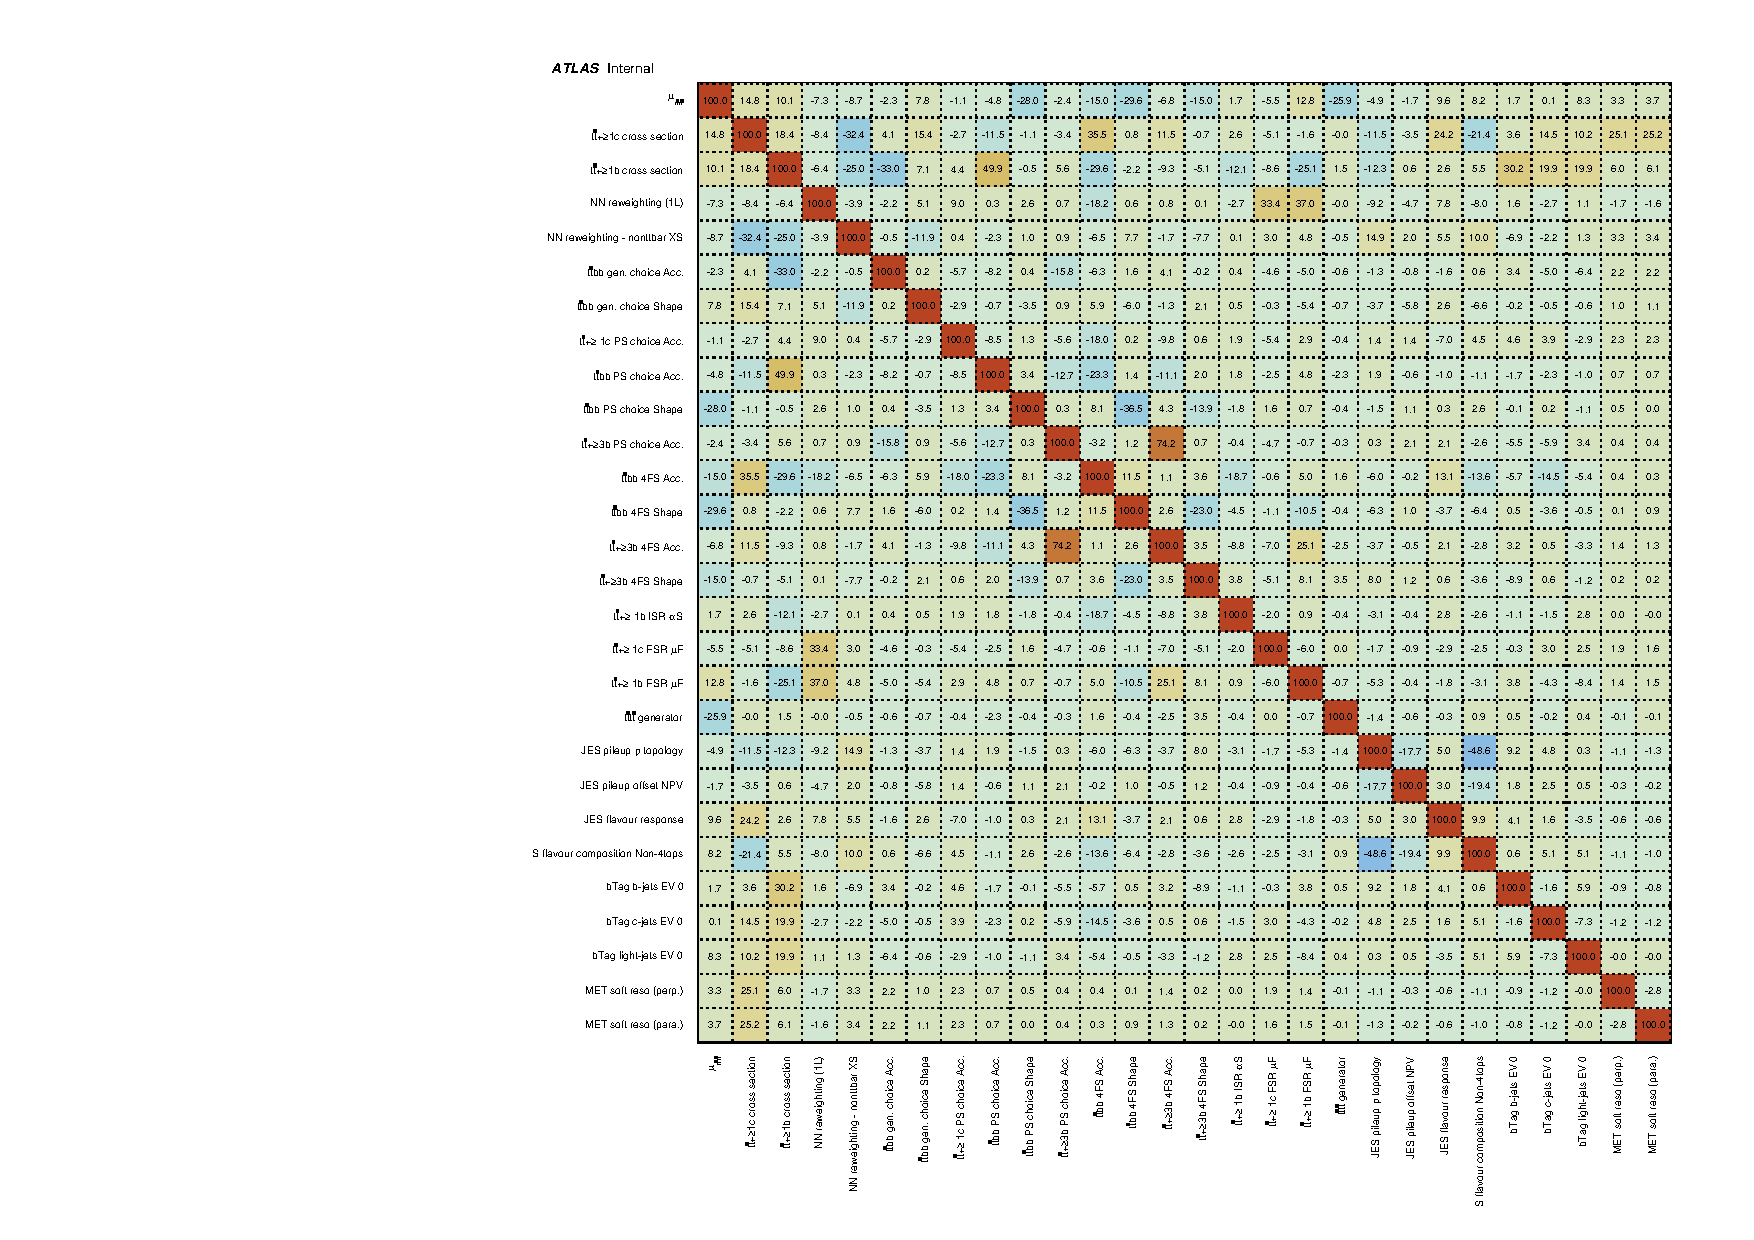
\includegraphics[width=\linewidth]{figures/fits/GNN/700/1L/asimov/CorrMatrix.pdf}
        \caption{\label{fig:Corr_mH700_Asimov_1L}Correlation matrix for the 1L Asimov fit for mH = 700 GeV}
\end{figure}

\begin{figure}[htbp!]
        \centering
        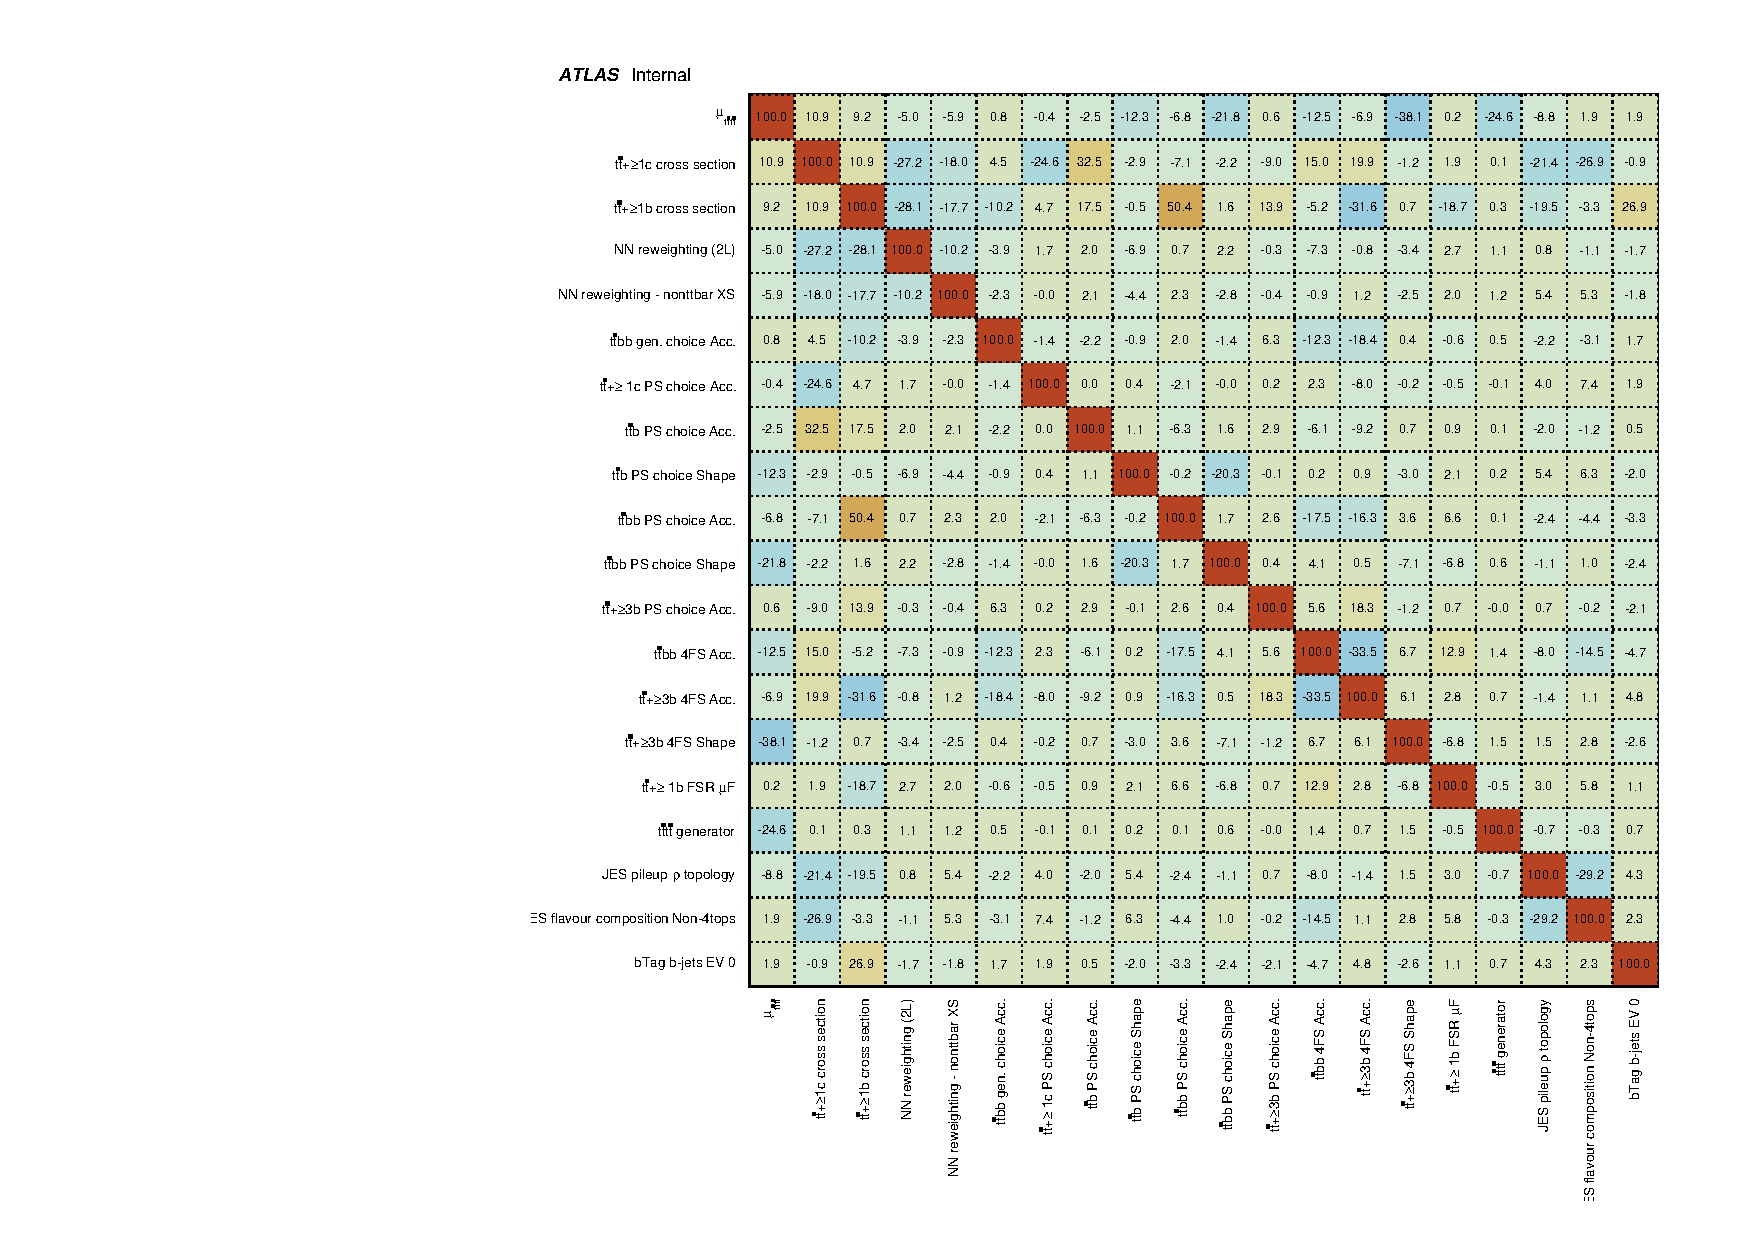
\includegraphics[width=\linewidth]{figures/fits/GNN/700/2L/asimov/CorrMatrix.pdf}
        \caption{\label{fig:Corr_mH700_Asimov_2L}Correlation matrix for the 2LOS Asimov fit for mH = 700 GeV}
\end{figure}

\begin{figure}[htbp!]
        \centering
        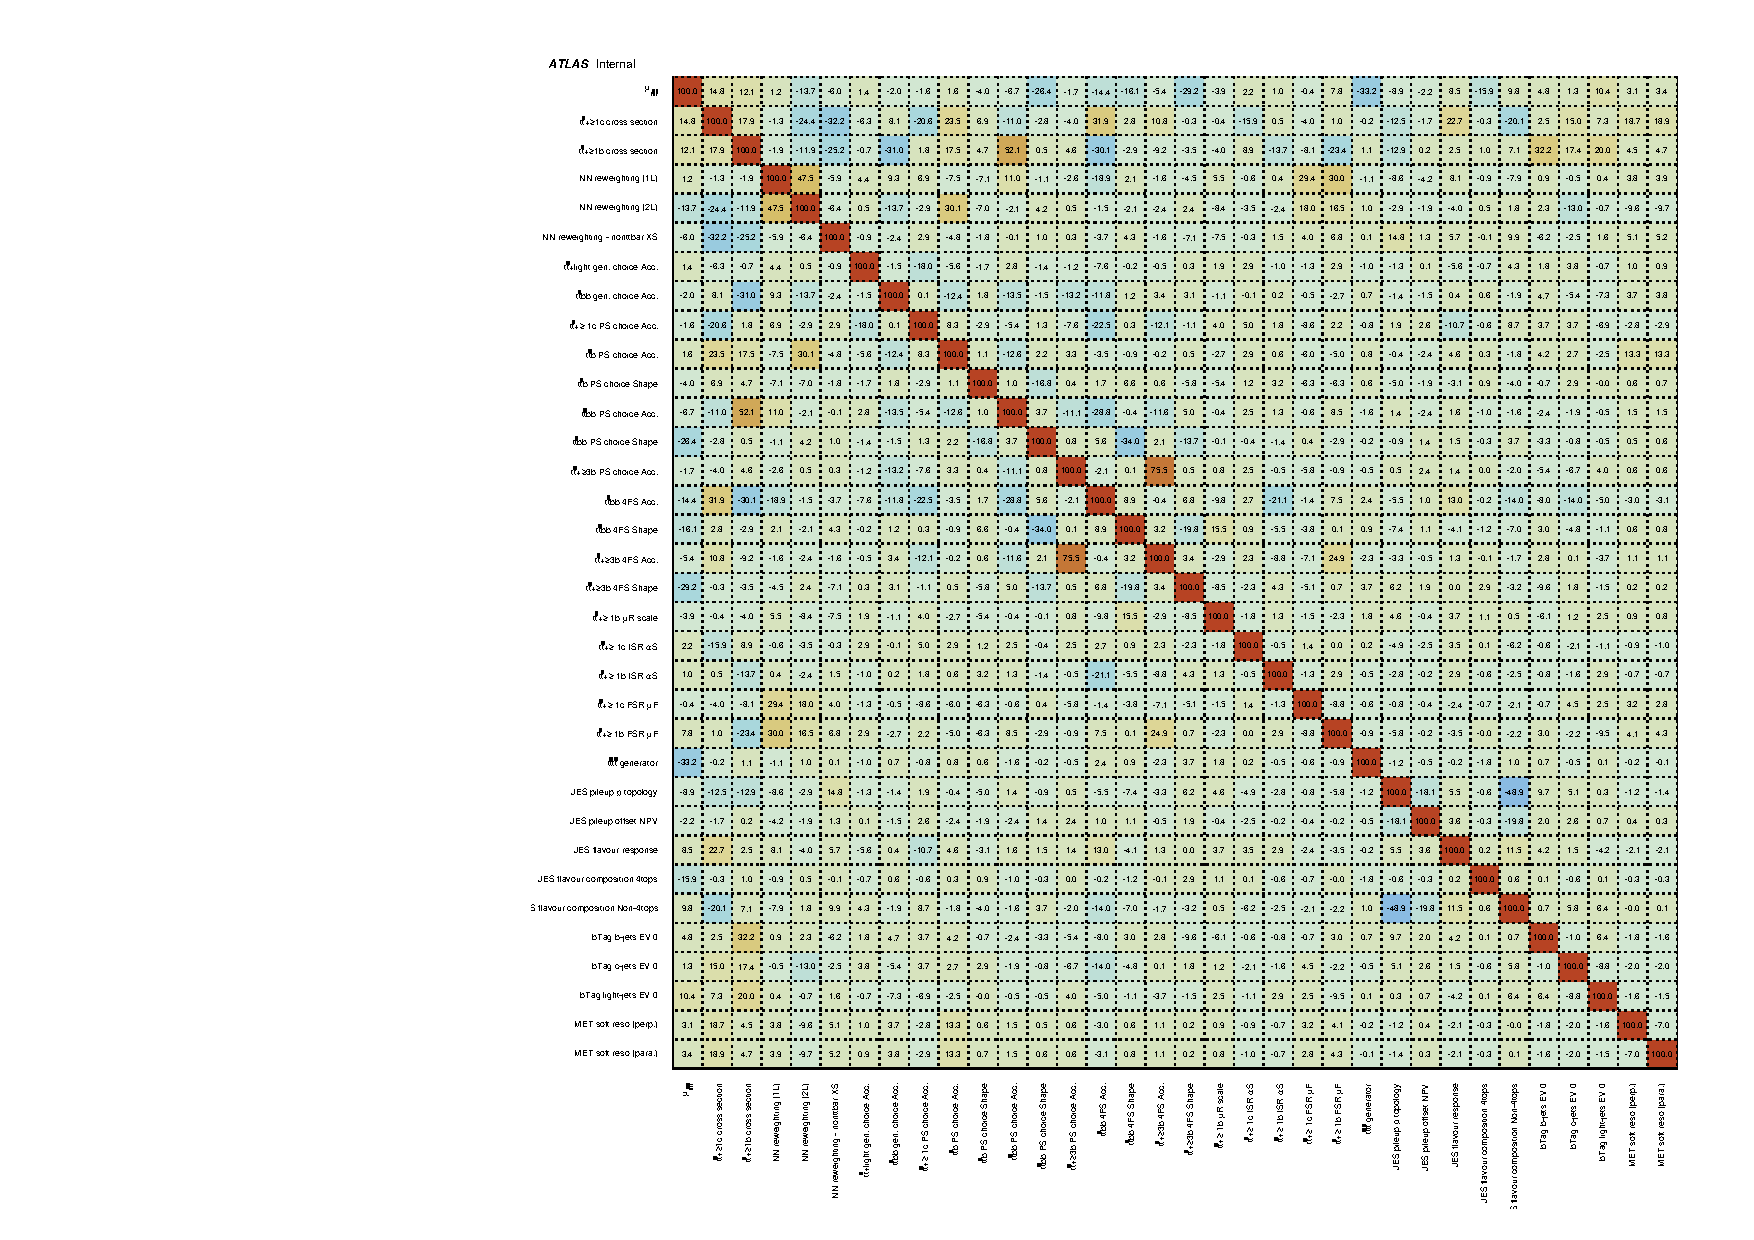
\includegraphics[width=\linewidth]{figures/fits/GNN/700/all/asimov/CorrMatrix.pdf}
        \caption{\label{fig:Corr_mH700_Asimov_all}Correlation matrix for the 1L/2LOS combined Asimov fit for mH = 700 GeV}
\end{figure}


\begin{figure}[htbp!]
        \centering
        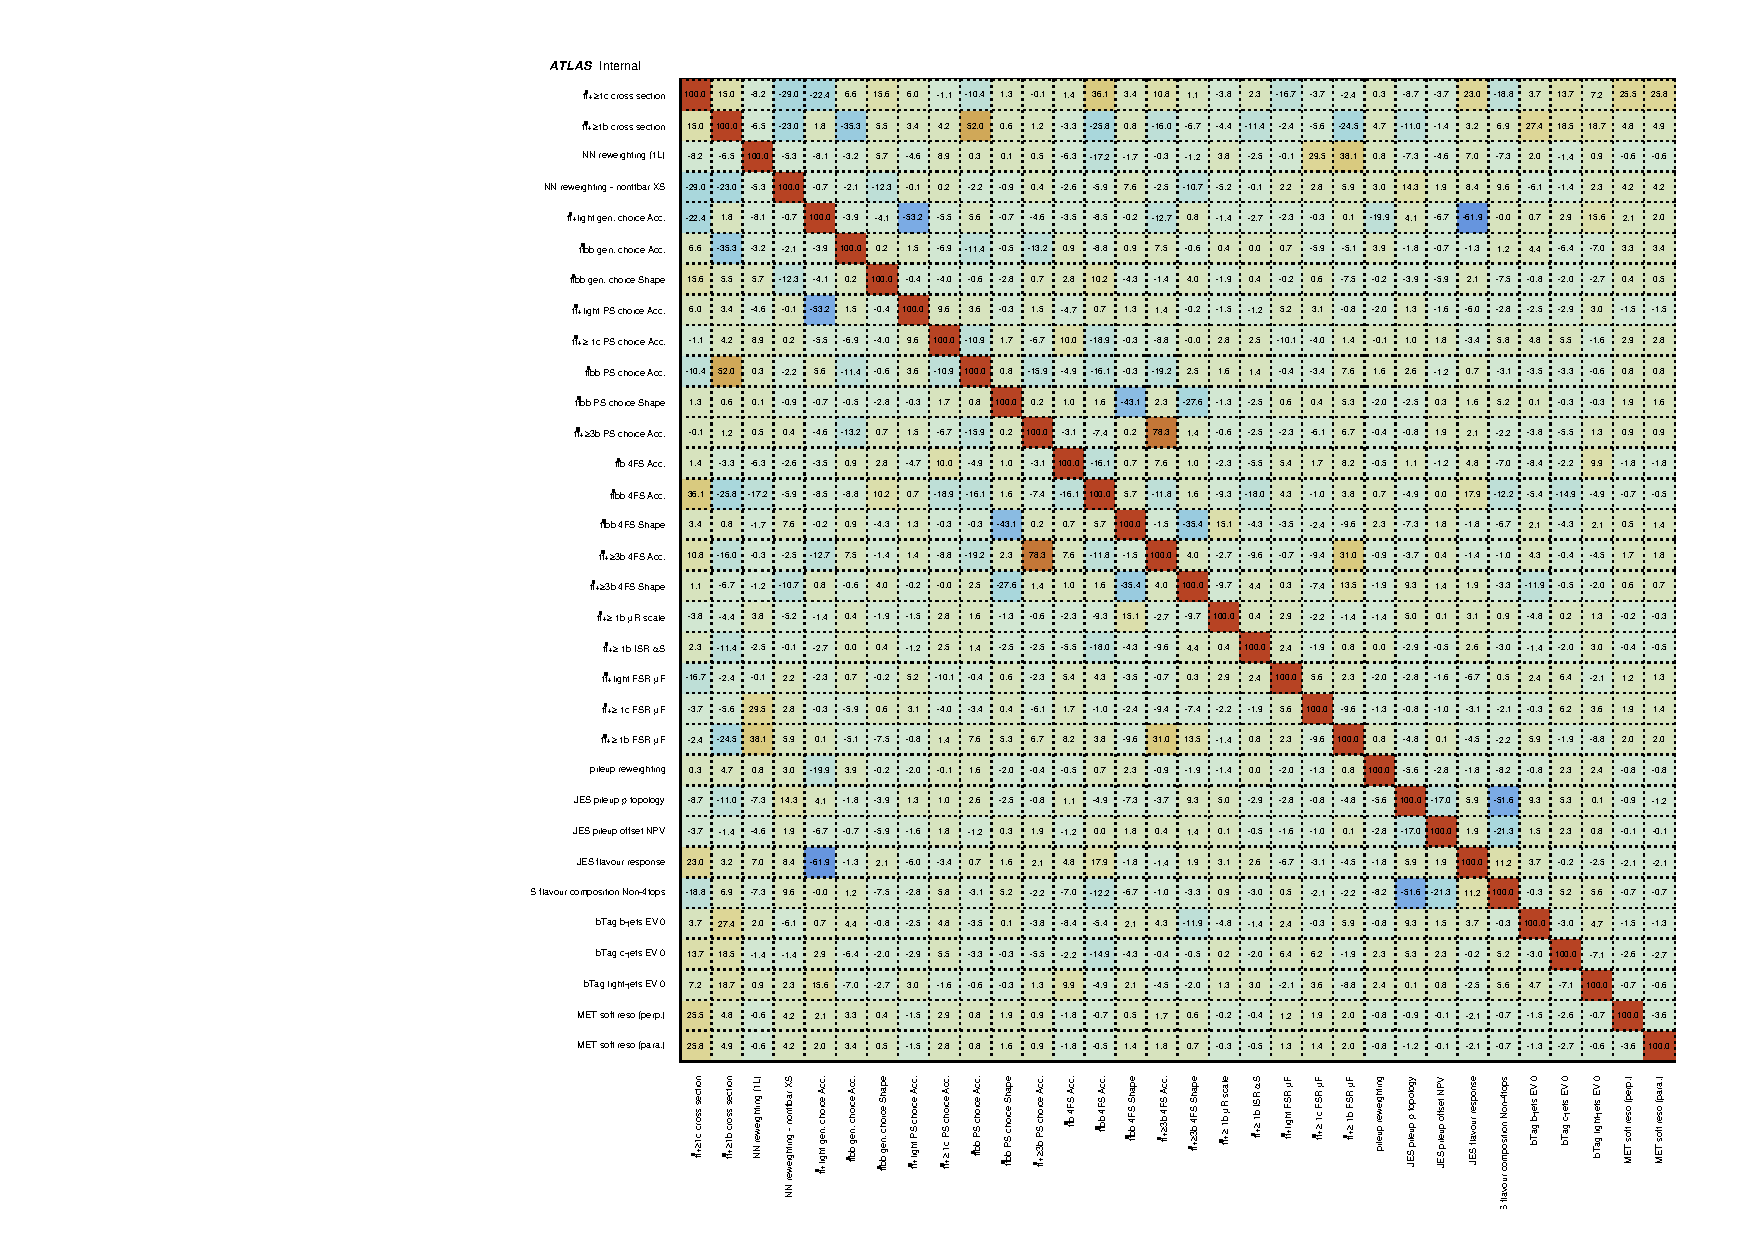
\includegraphics[width=\linewidth]{figures/fits/GNN/700/1L/data_unblindedBonly/CorrMatrix.pdf}
        \caption{\label{fig:Corr_mH700_Data_1L}Correlation matrix for the 1L blinded data fit for mH = 700 GeV}
\end{figure}

\begin{figure}[htbp!]
        \centering
        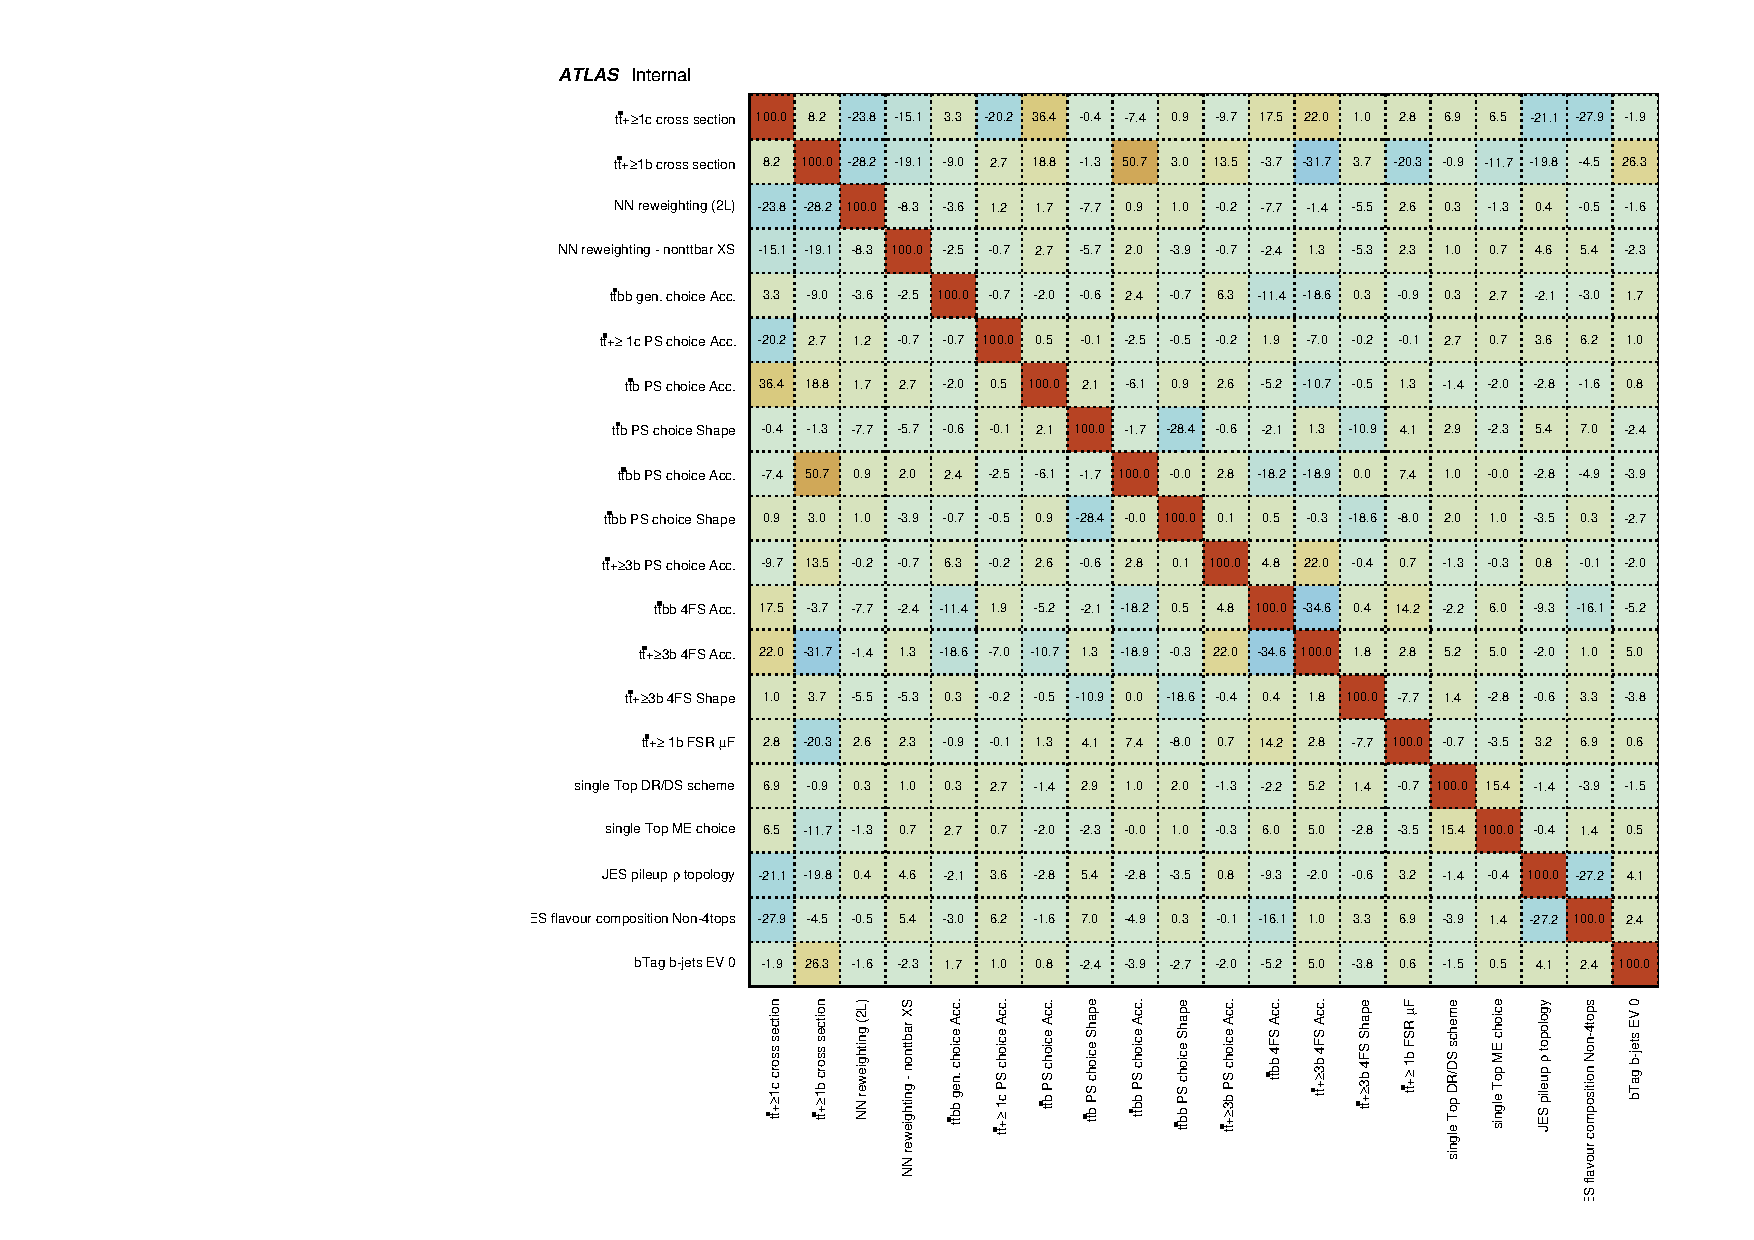
\includegraphics[width=\linewidth]{figures/fits/GNN/700/2L/data_unblindedBonly/CorrMatrix.pdf}
        \caption{\label{fig:Corr_mH700_Data_2L}Correlation matrix for the 2LOS blinded data fit for mH = 700 GeV}
\end{figure}

\begin{figure}[htbp!]
        \centering
        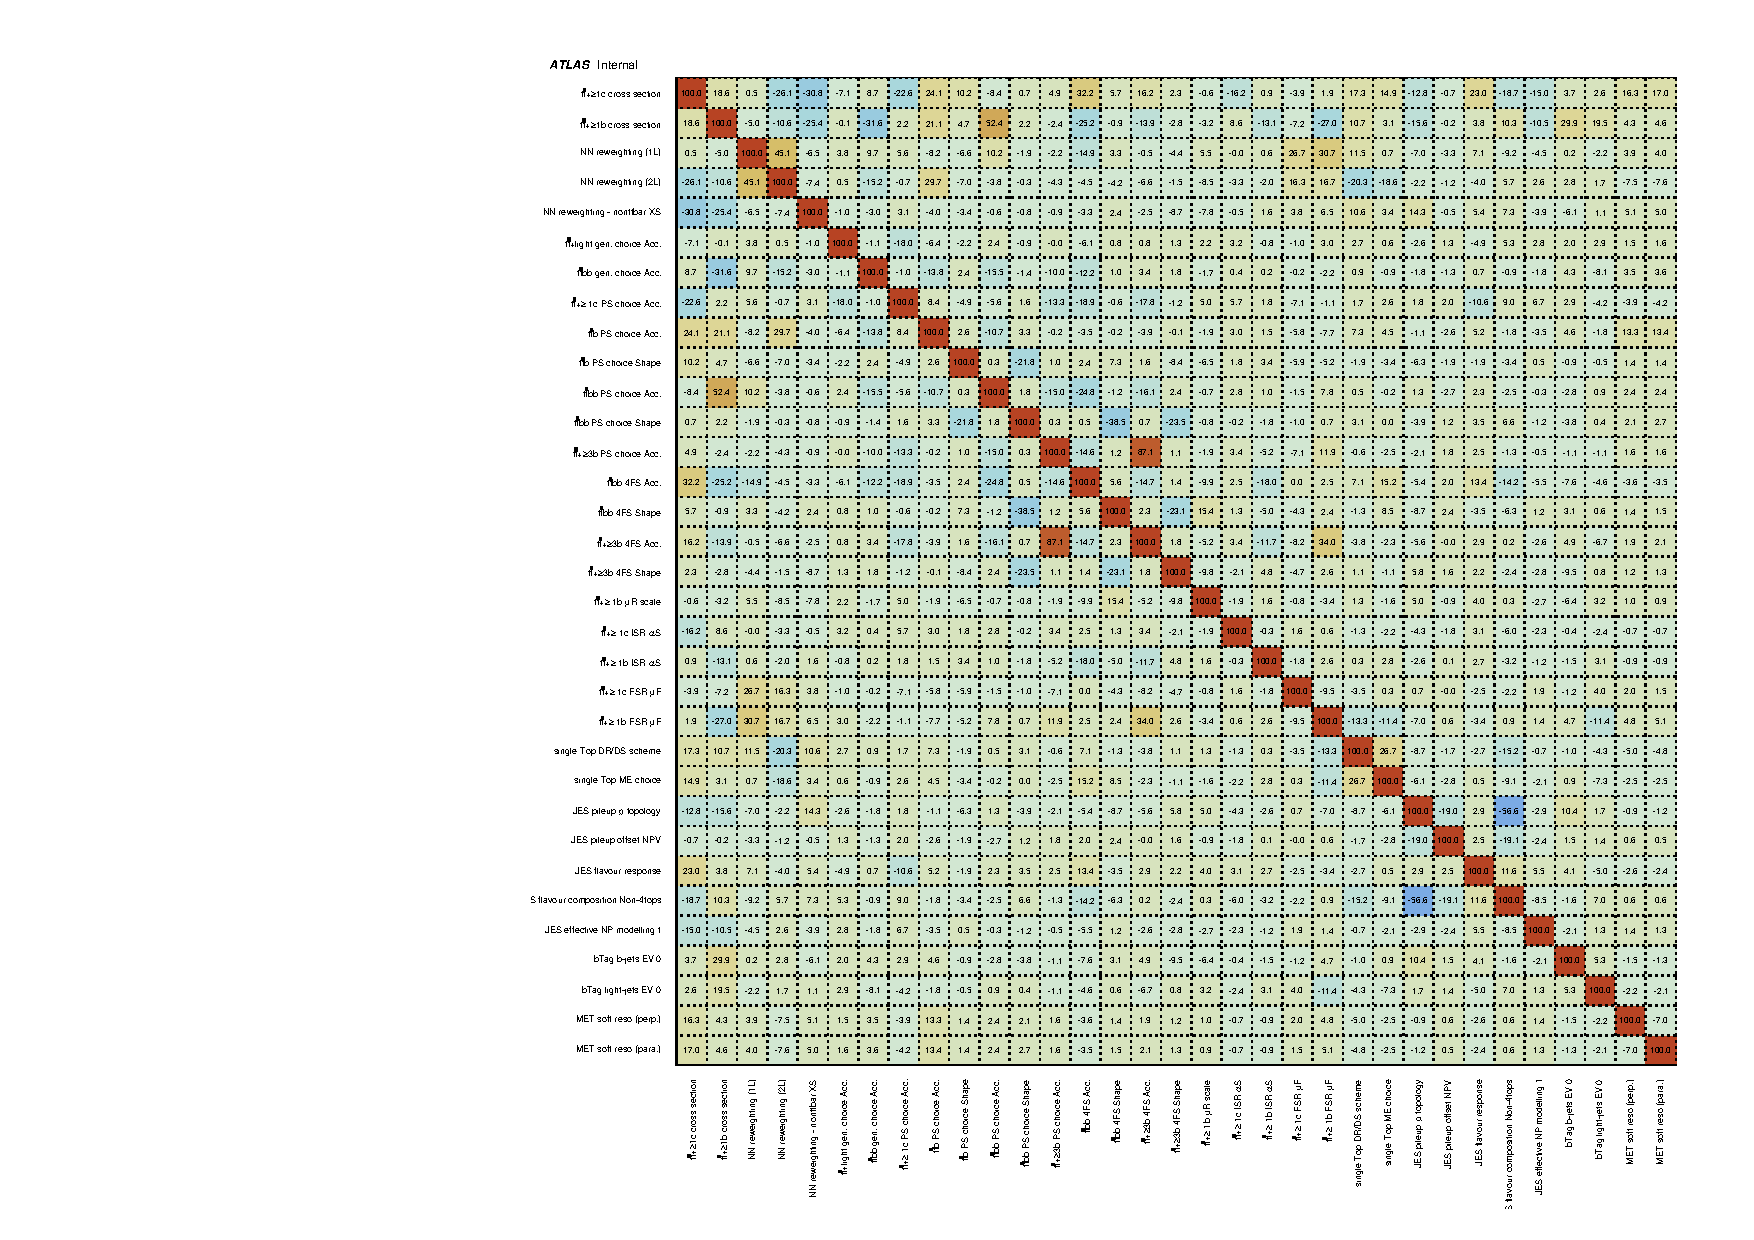
\includegraphics[width=\linewidth]{figures/fits/GNN/700/all/data_unblindedBonly/CorrMatrix.pdf}
        \caption{\label{fig:Corr_mH700_Data_all}Correlation matrix for the 1L/2LOS combined blinded data fit for mH = 700 GeV}
\end{figure}


\begin{figure}[htbp!]
        \begin{center} \setlength{\tabcolsep}{2.5pt}\footnotesize
        \begin{tabular}{cccc}

        &
        &
        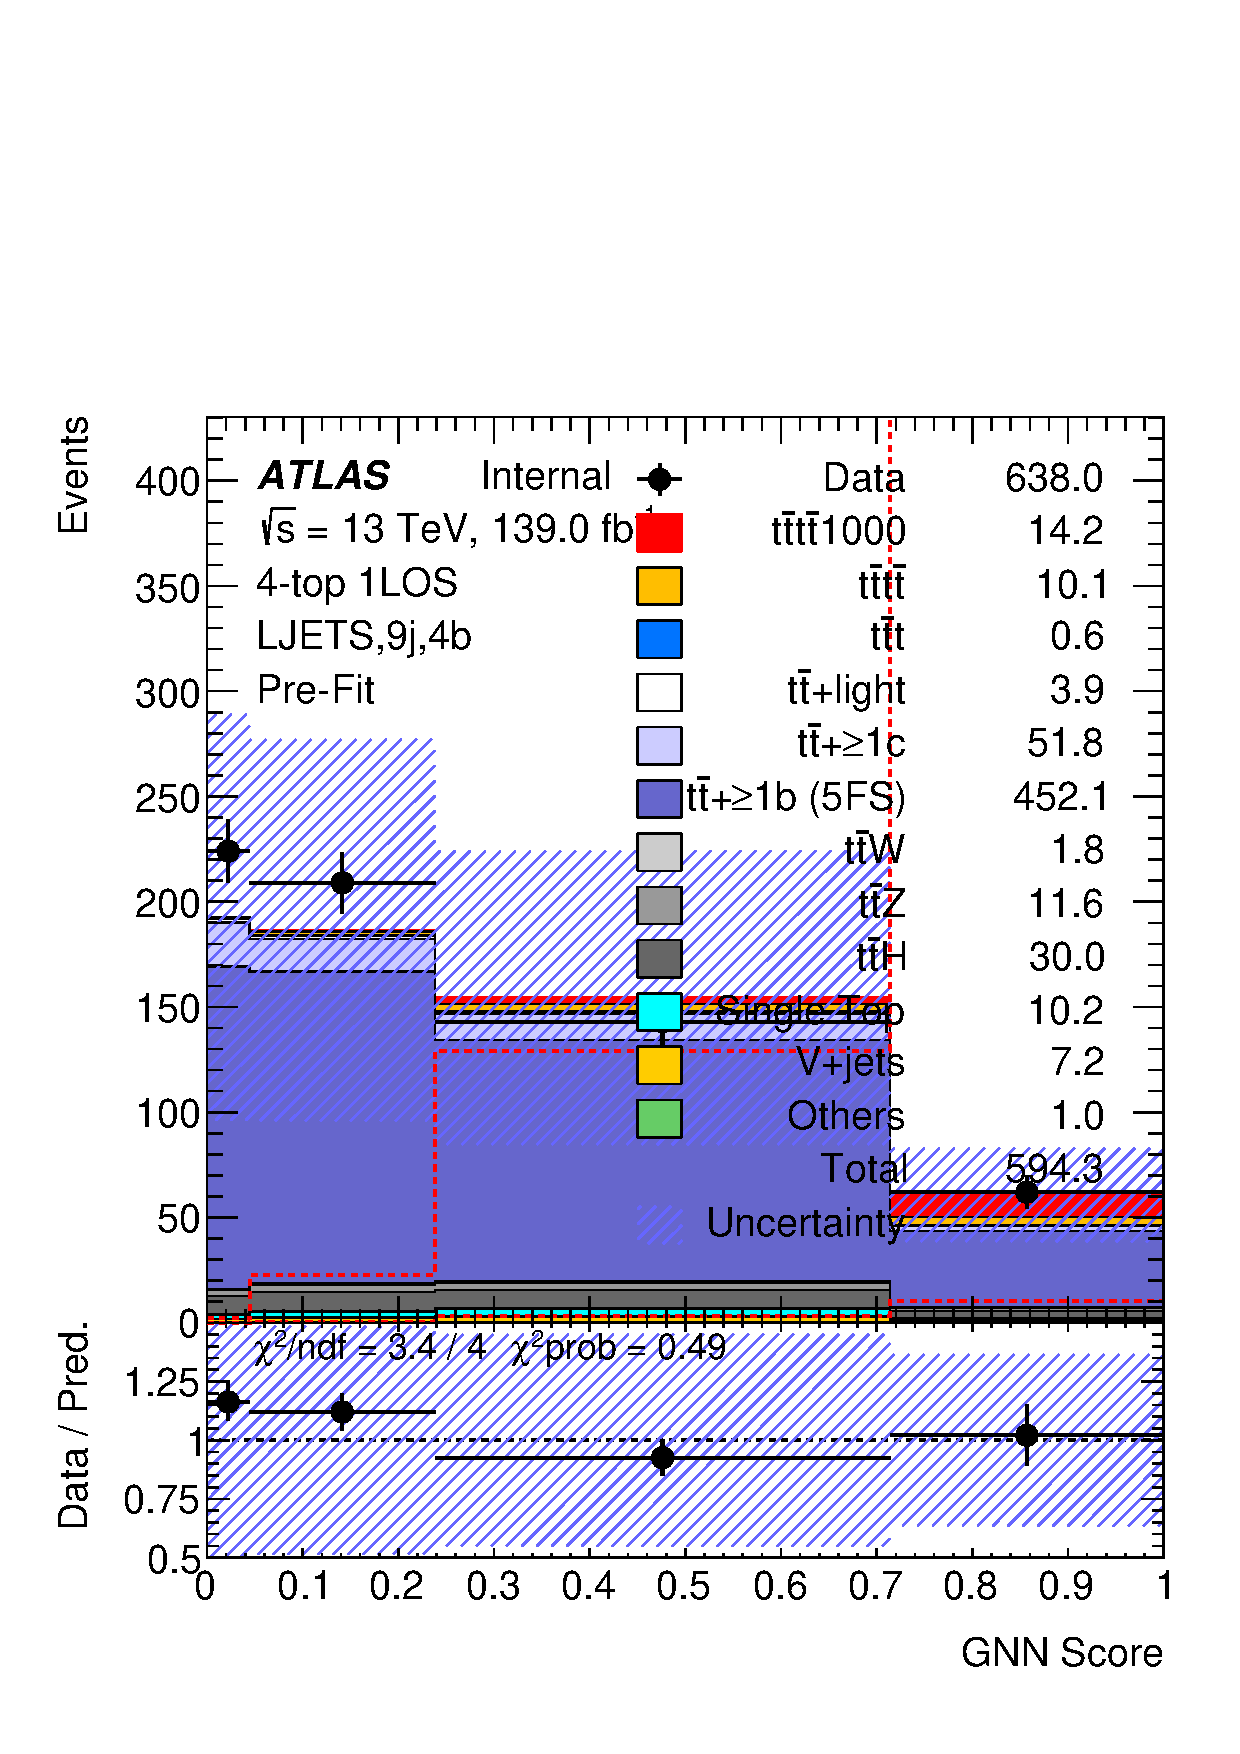
\includegraphics[width=0.23 \textwidth]{figures/fits/GNN/1000/all/data_unblindedBonly/Plots/ljets_9j4b.pdf} &
        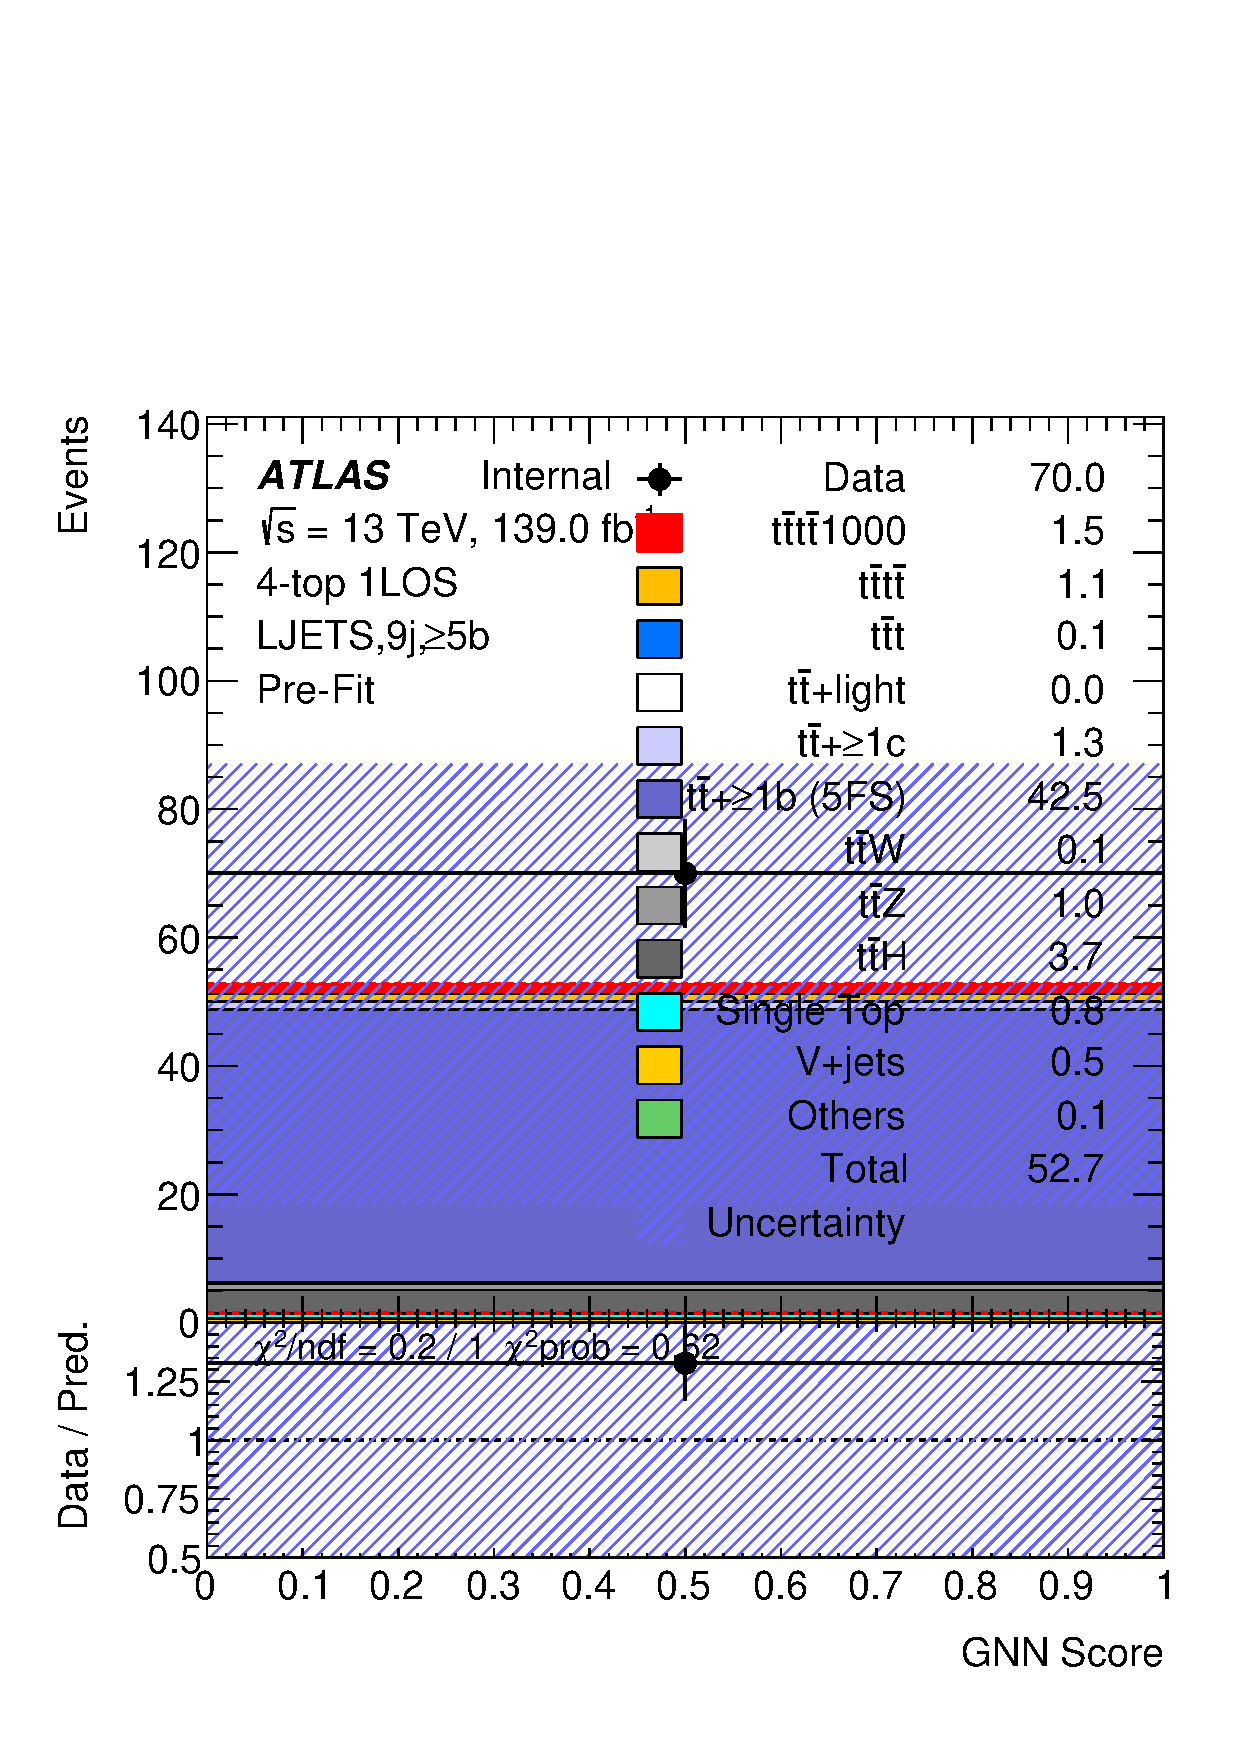
\includegraphics[width=0.23 \textwidth]{figures/fits/GNN/1000/all/data_unblindedBonly/Plots/ljets_9jge5b.pdf} \\

        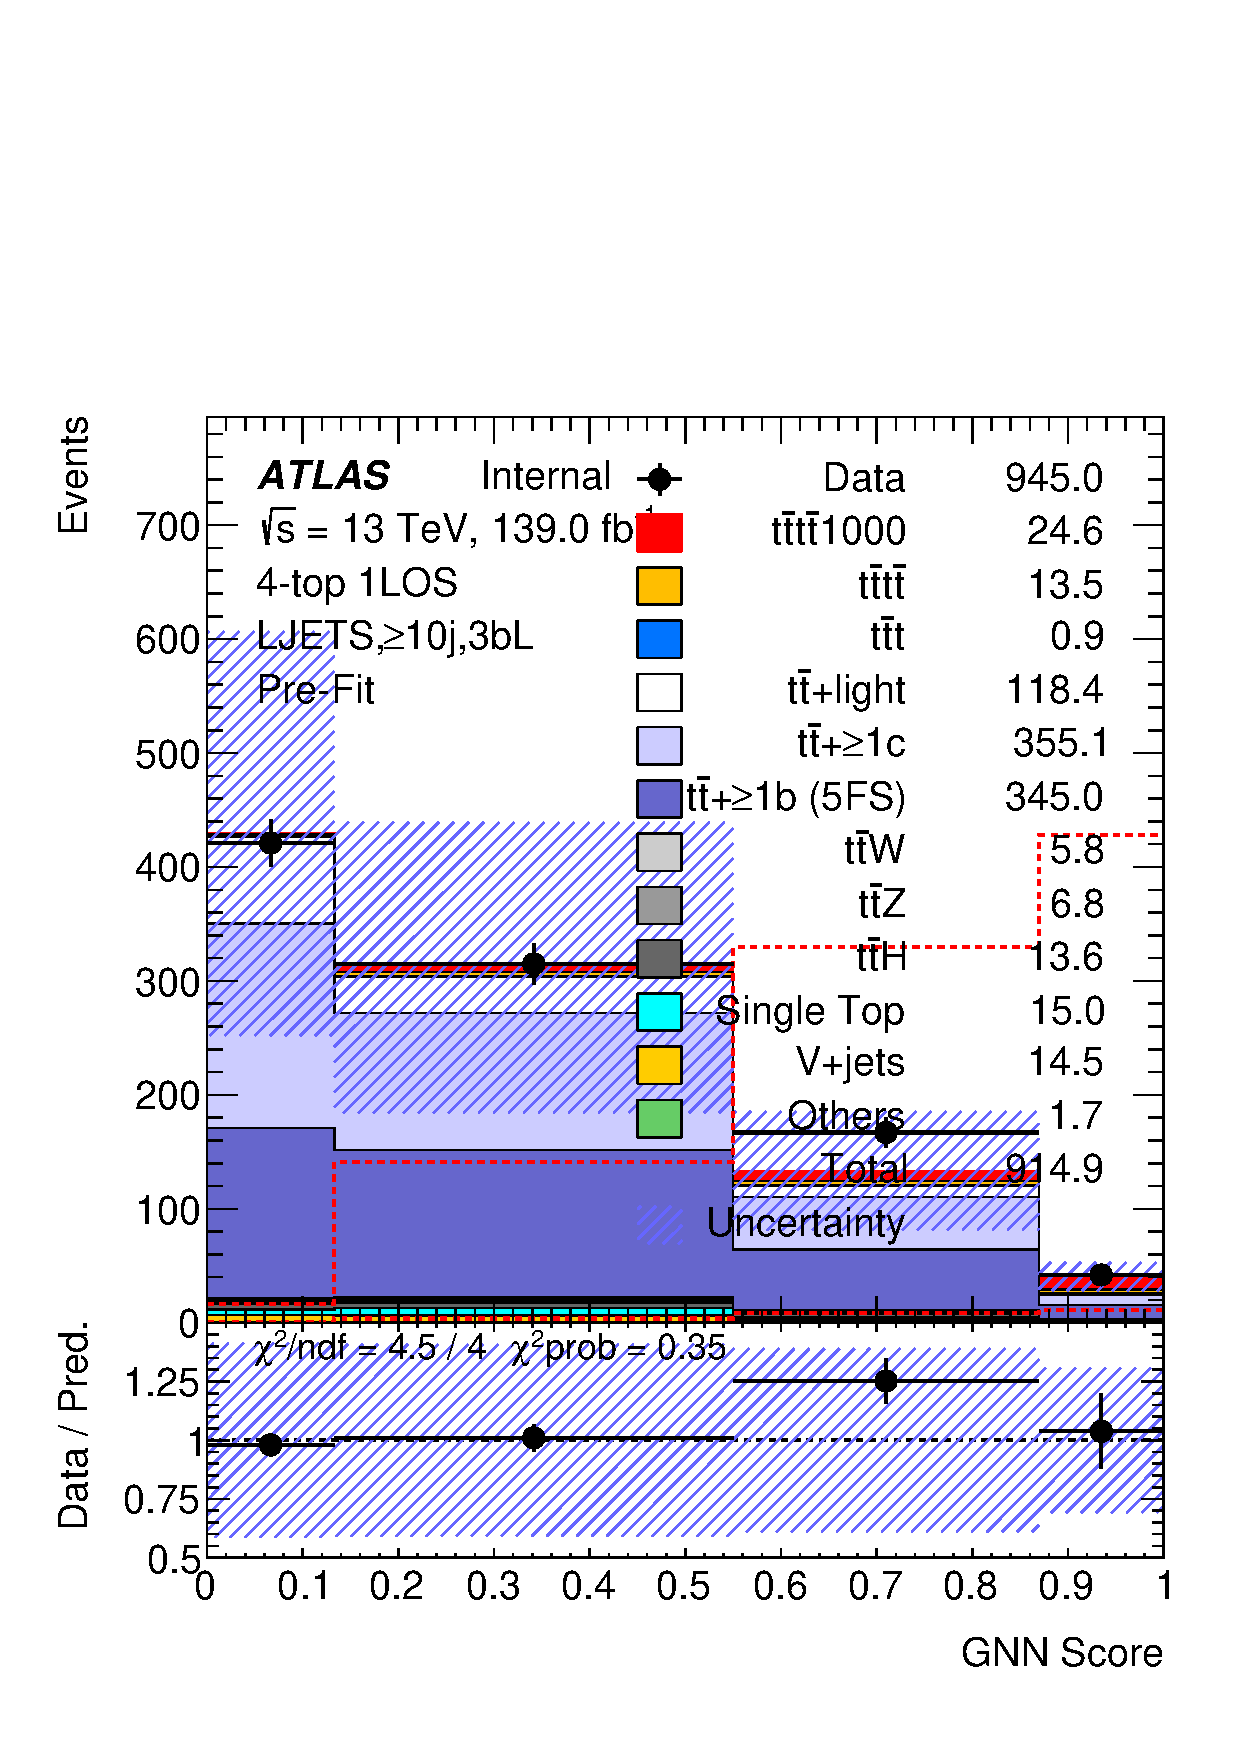
\includegraphics[width=0.23 \textwidth]{figures/fits/GNN/1000/all/data_unblindedBonly/Plots/ljets_ge10j3bL.pdf} &
        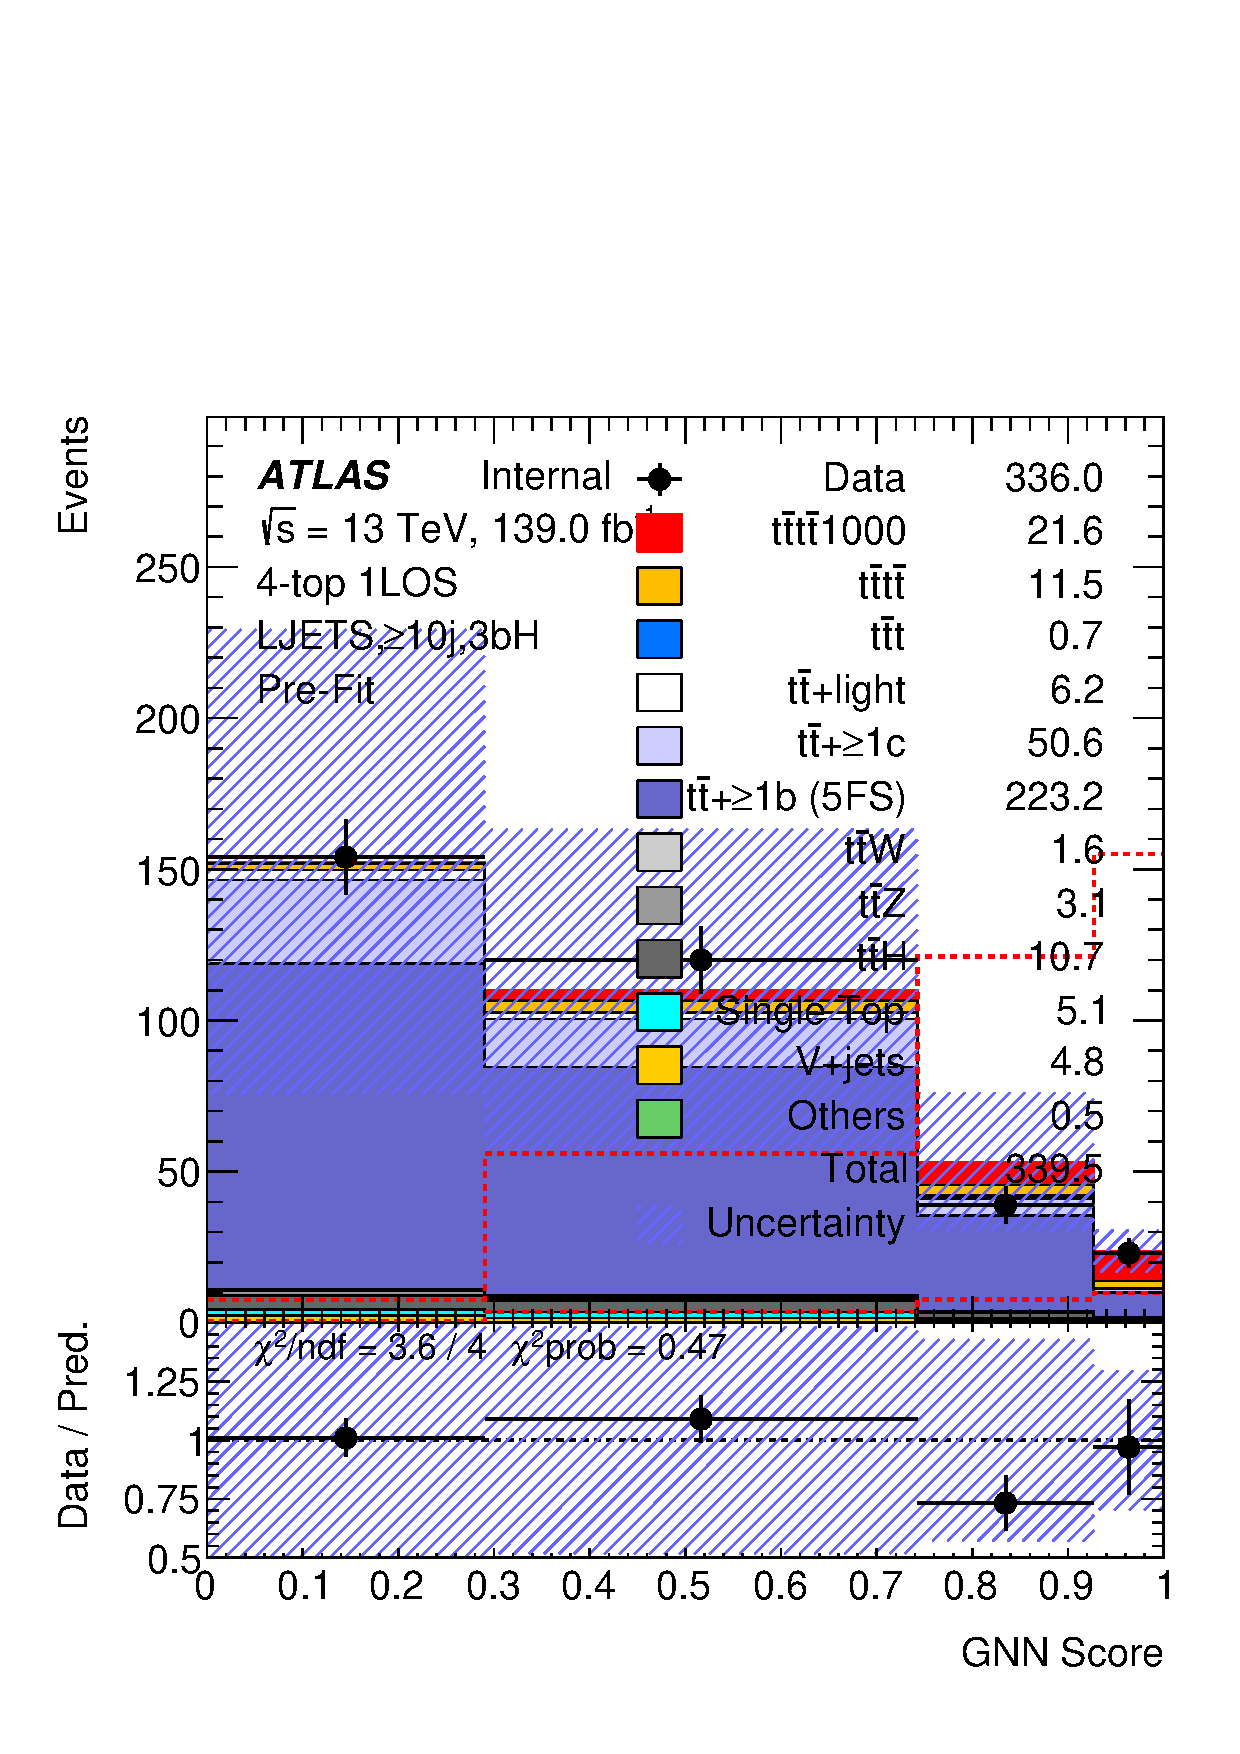
\includegraphics[width=0.23 \textwidth]{figures/fits/GNN/1000/all/data_unblindedBonly/Plots/ljets_ge10j3bH.pdf} &
        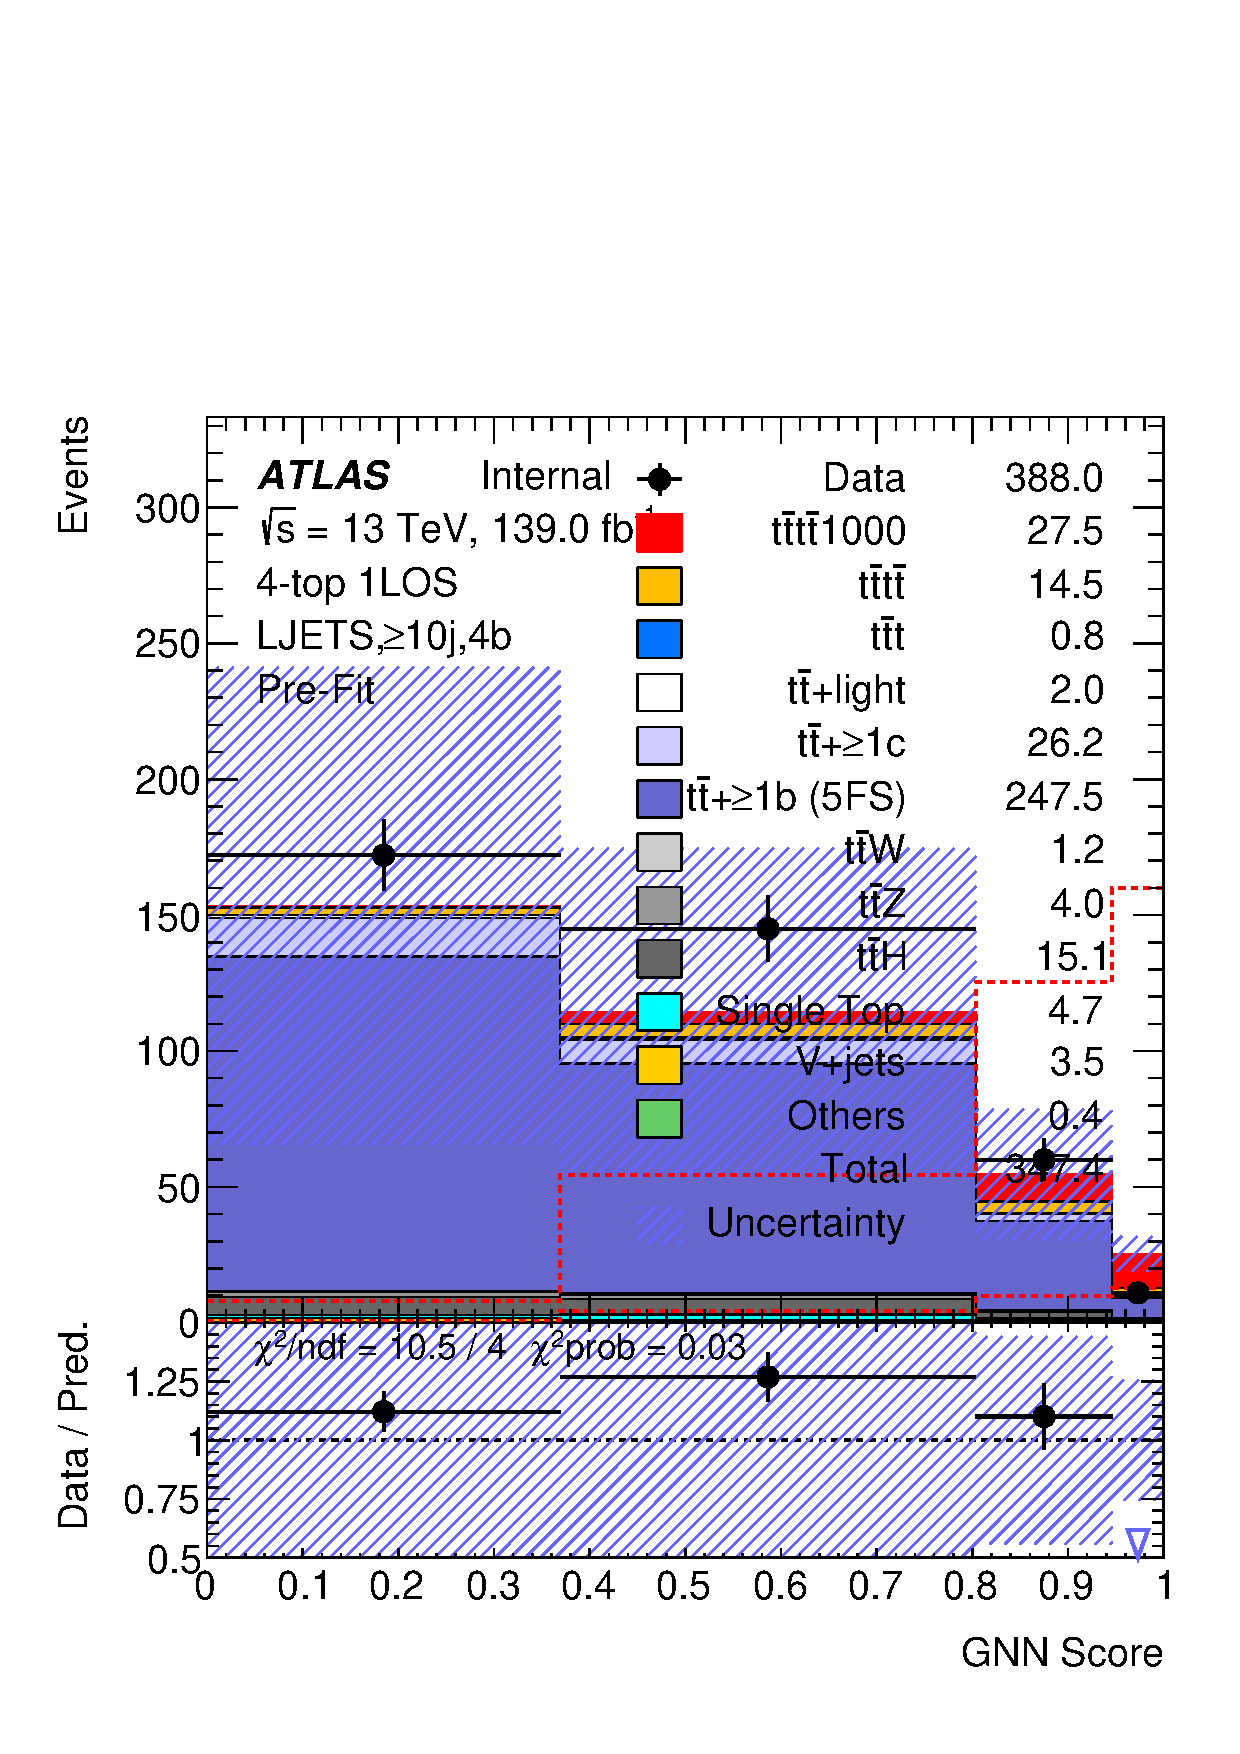
\includegraphics[width=0.23 \textwidth]{figures/fits/GNN/1000/all/data_unblindedBonly/Plots/ljets_ge10j4b.pdf} &
        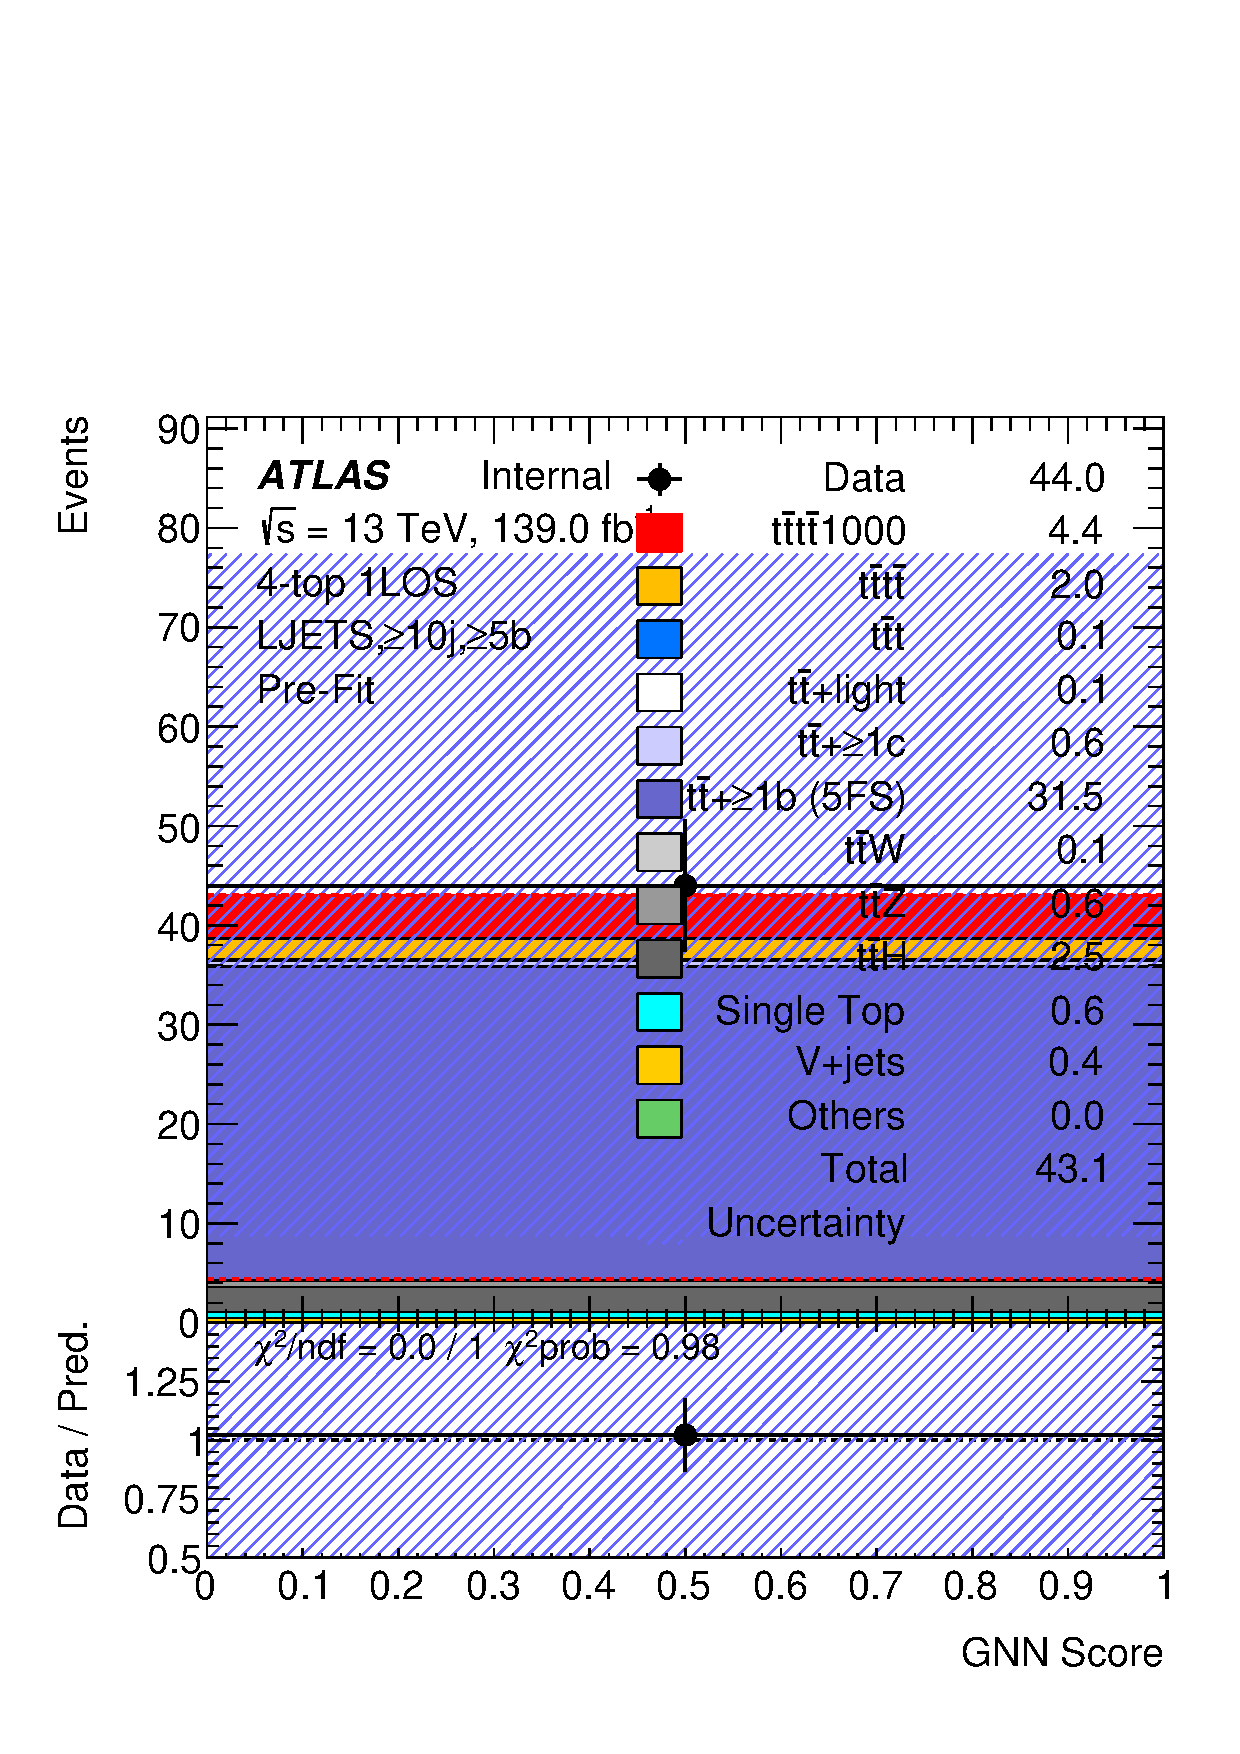
\includegraphics[width=0.23 \textwidth]{figures/fits/GNN/1000/all/data_unblindedBonly/Plots/ljets_ge10jge5b.pdf} \\
        \end{tabular}
        \caption{\label{fig:Prefit_Yields_1L_1000GeV}Pre-fit distributions for 1L signal regions associated with different signal and background samples, compared with data yields for mH = 1000 GeV.}
\end{center}
\end{figure}

\begin{figure}[htbp!]
        \begin{center} \setlength{\tabcolsep}{2.5pt}\footnotesize
        \begin{tabular}{ccc}

        &
        &
        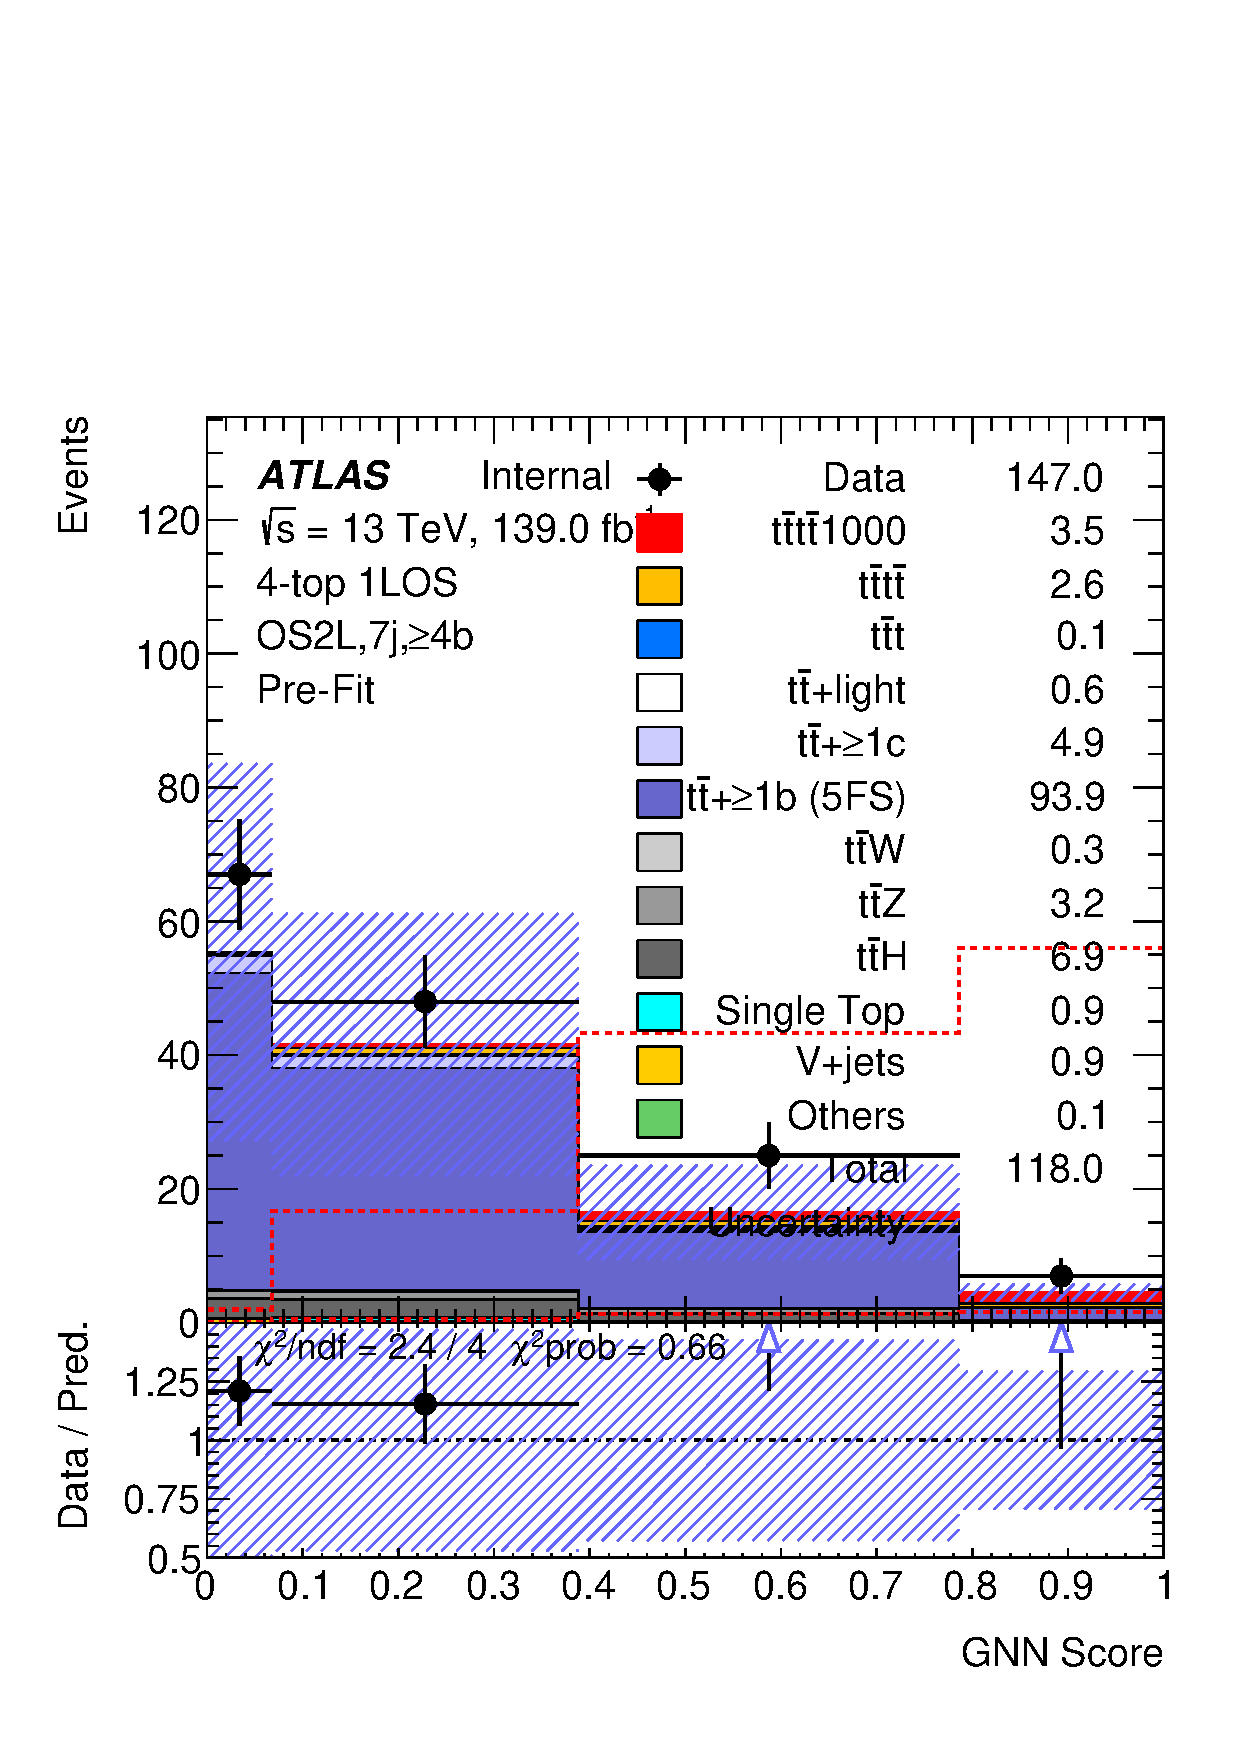
\includegraphics[width=0.31 \textwidth]{figures/fits/GNN/1000/all/data_unblindedBonly/Plots/os2l_7jge4b.pdf} \\

        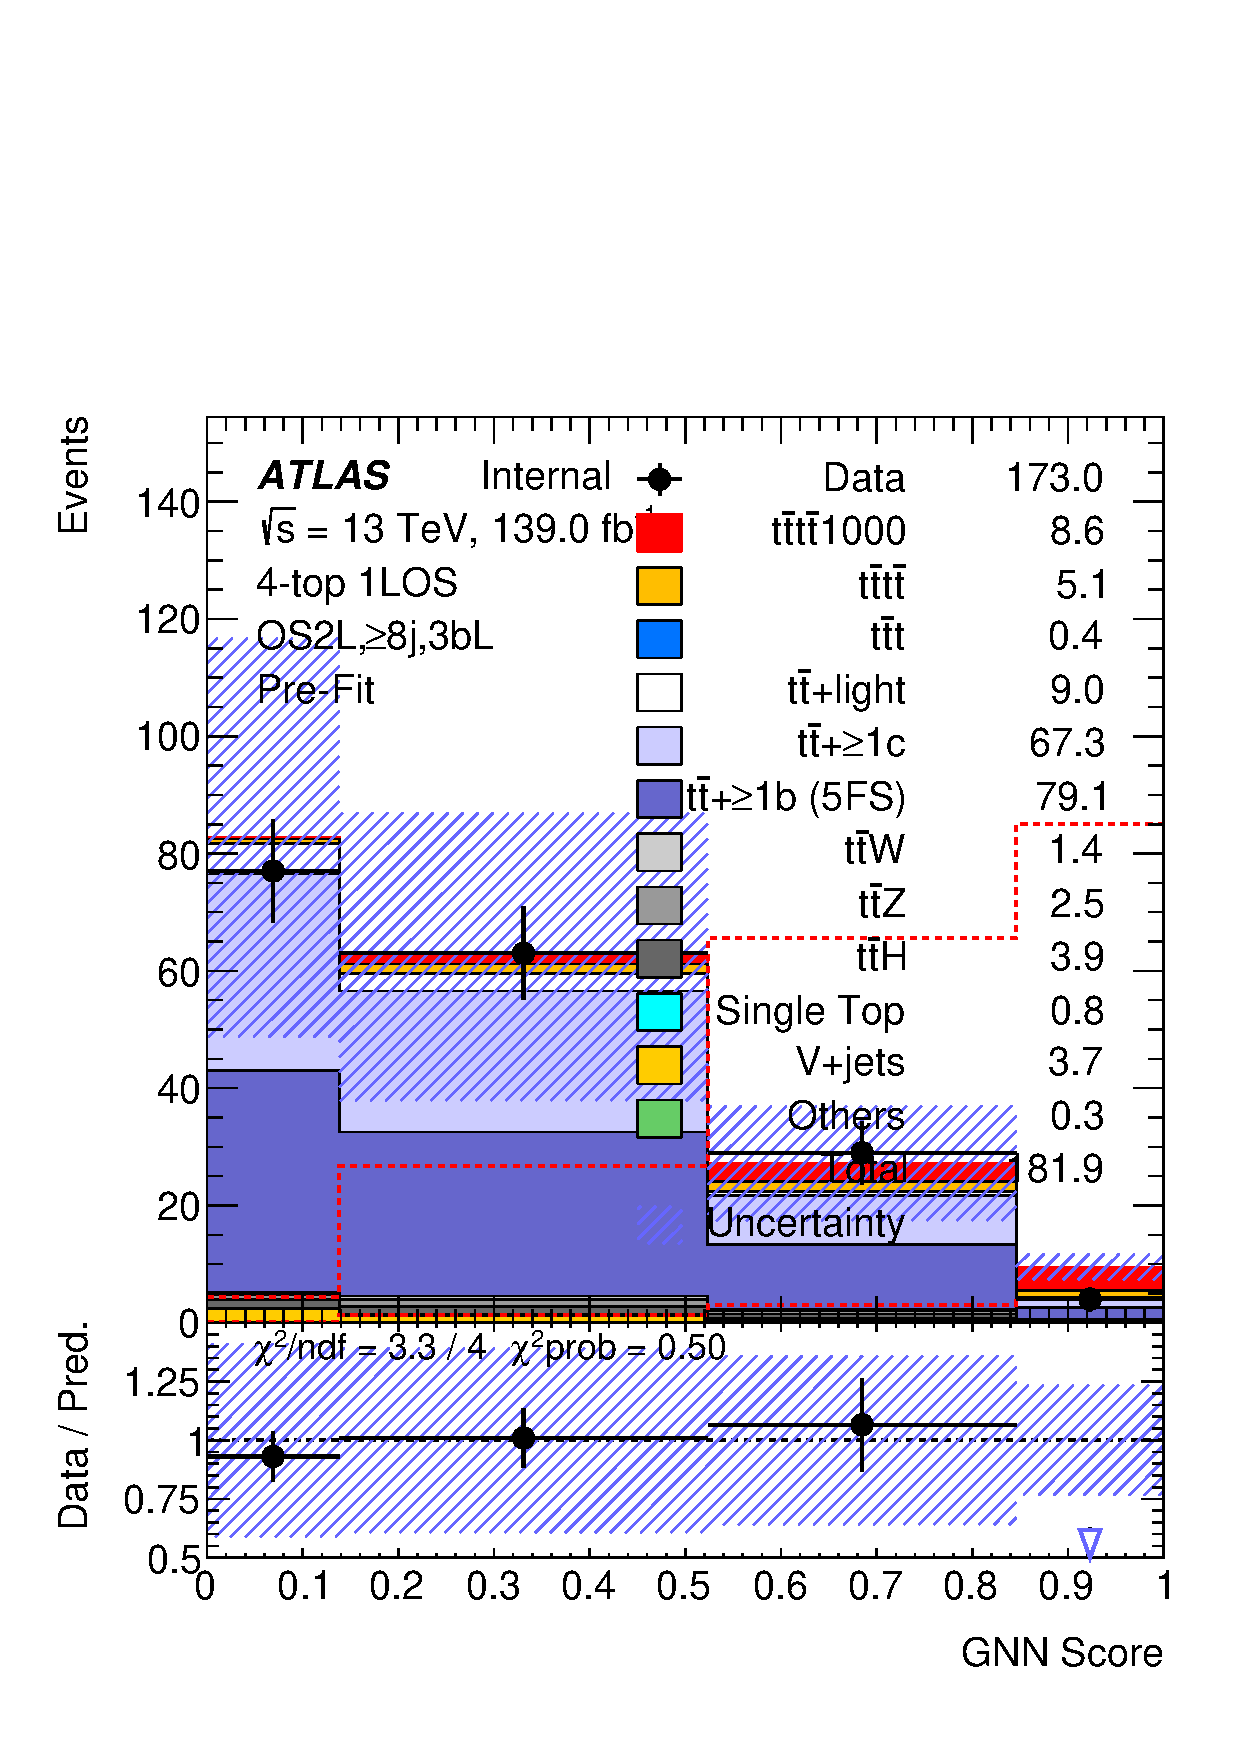
\includegraphics[width=0.31 \textwidth]{figures/fits/GNN/1000/all/data_unblindedBonly/Plots/os2l_ge8j3bL.pdf} &
        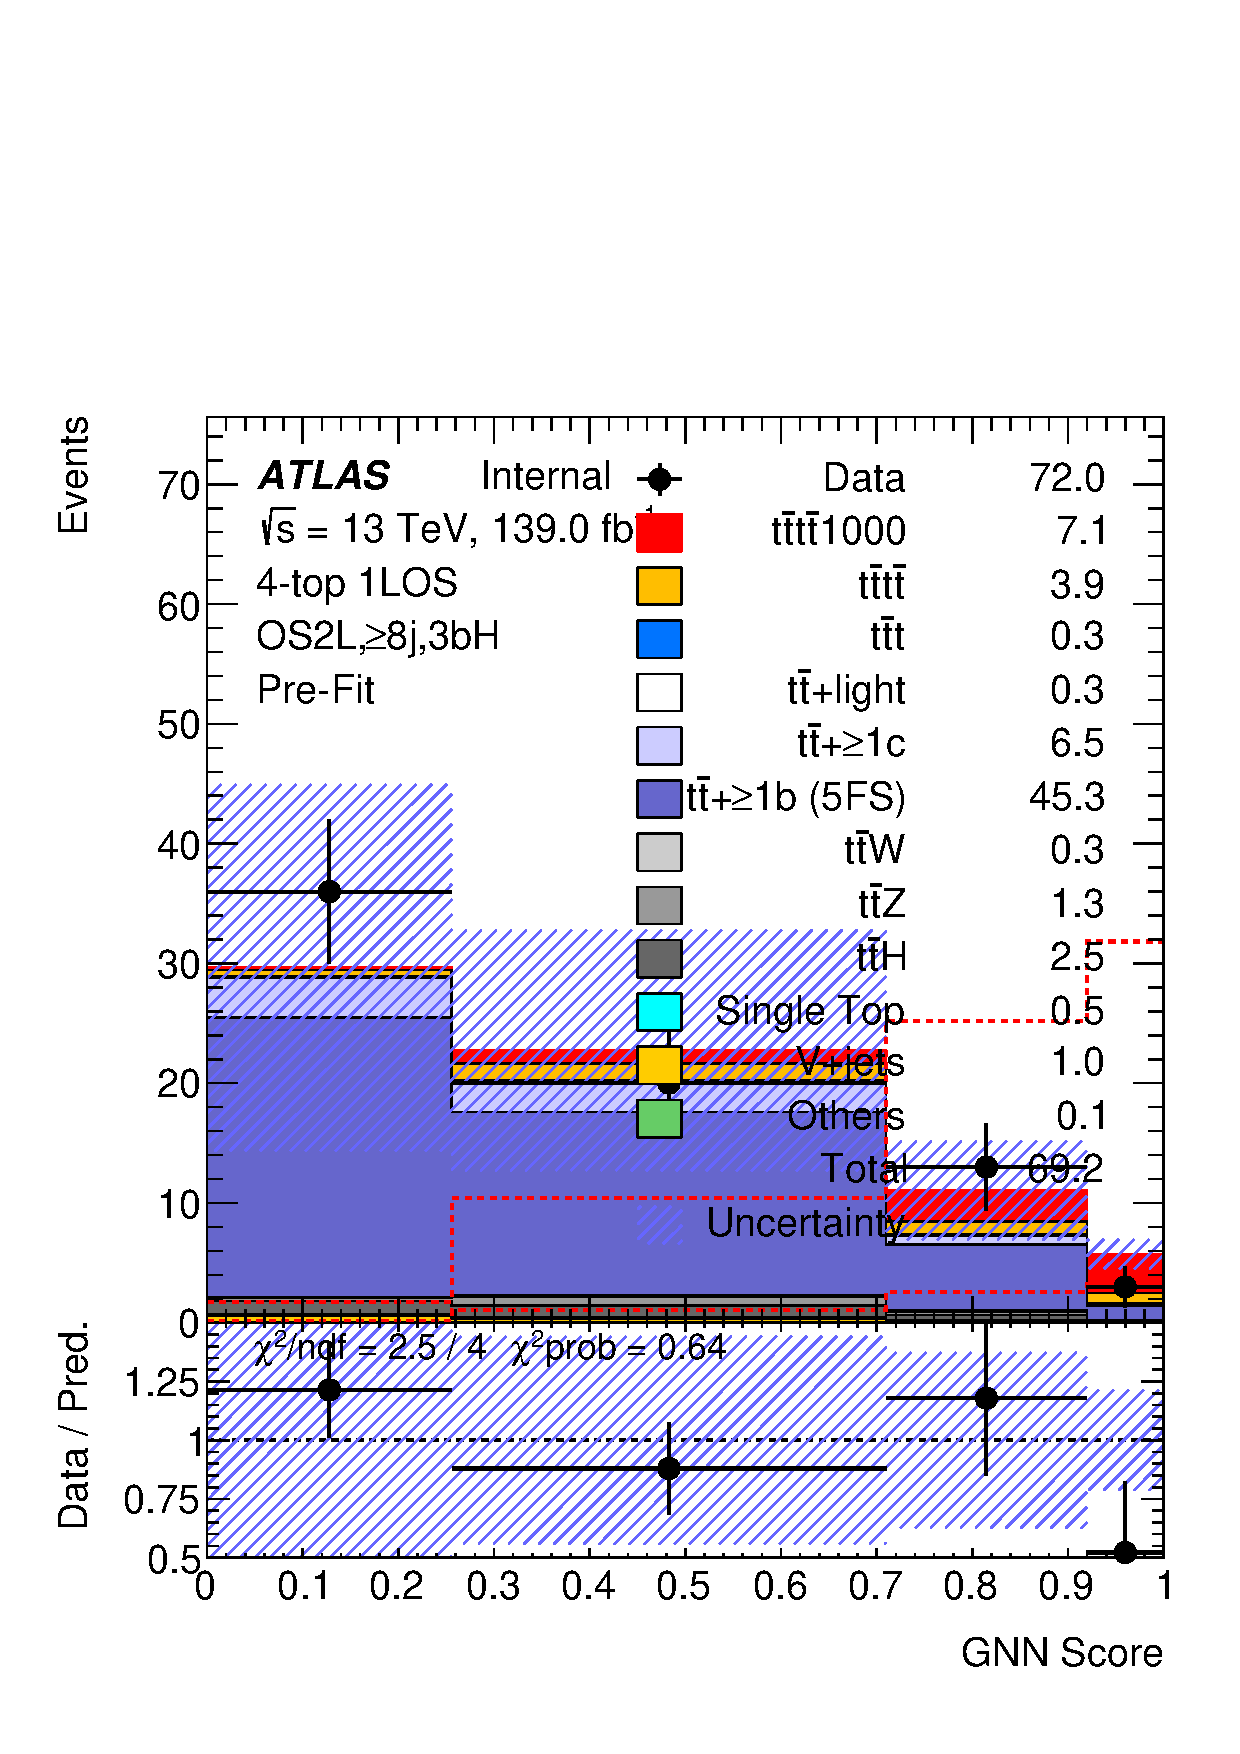
\includegraphics[width=0.31 \textwidth]{figures/fits/GNN/1000/all/data_unblindedBonly/Plots/os2l_ge8j3bH.pdf} &
        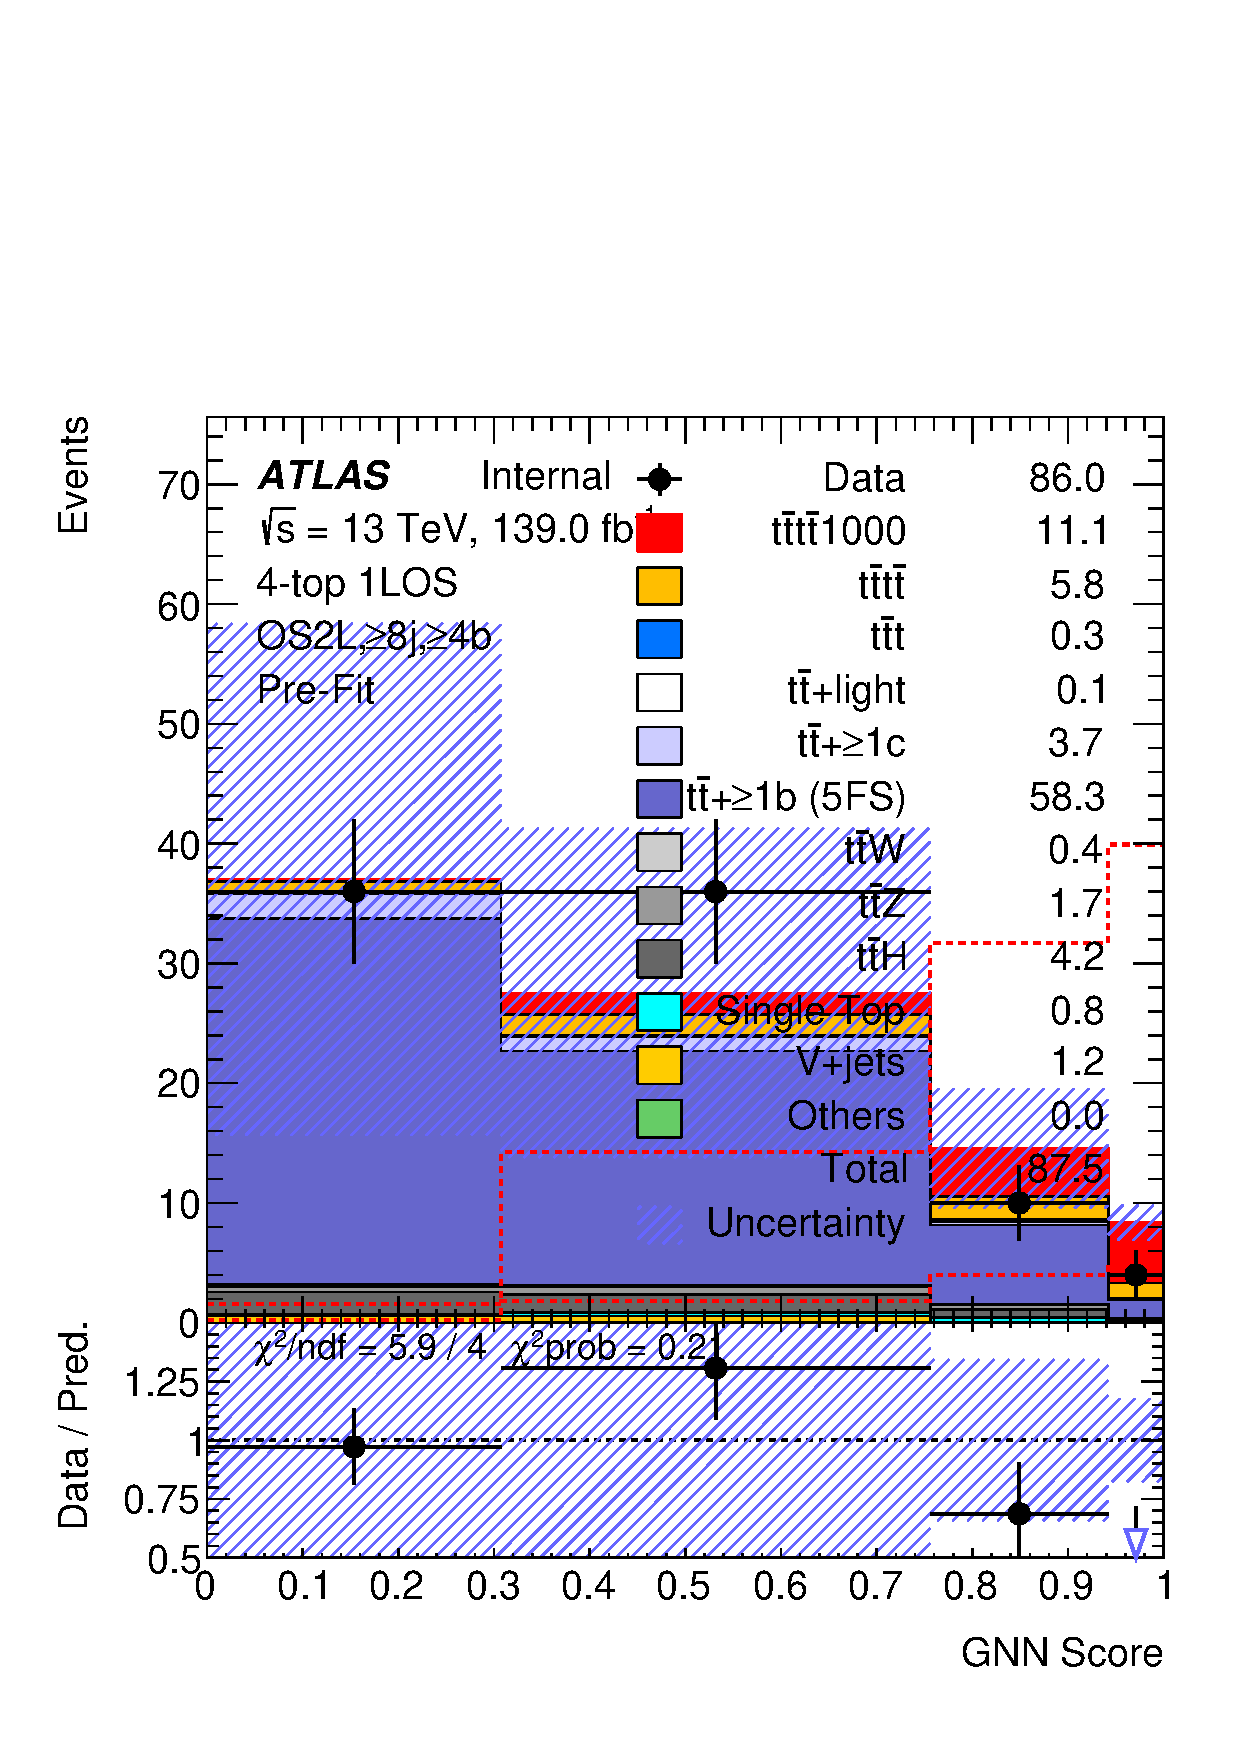
\includegraphics[width=0.31 \textwidth]{figures/fits/GNN/1000/all/data_unblindedBonly/Plots/os2l_ge8jge4b.pdf} \\
        \end{tabular}
        \caption{\label{fig:Prefit_Yields_2L_1000GeV}Pre-fit distributions for 2LOS signal regions associated with different signal and background samples, compared with data yields for mH = 1000 GeV.}
\end{center}
\end{figure}

\begin{figure}[htbp!]
        \begin{center} \setlength{\tabcolsep}{2.5pt}\footnotesize
        \begin{tabular}{cccc}
        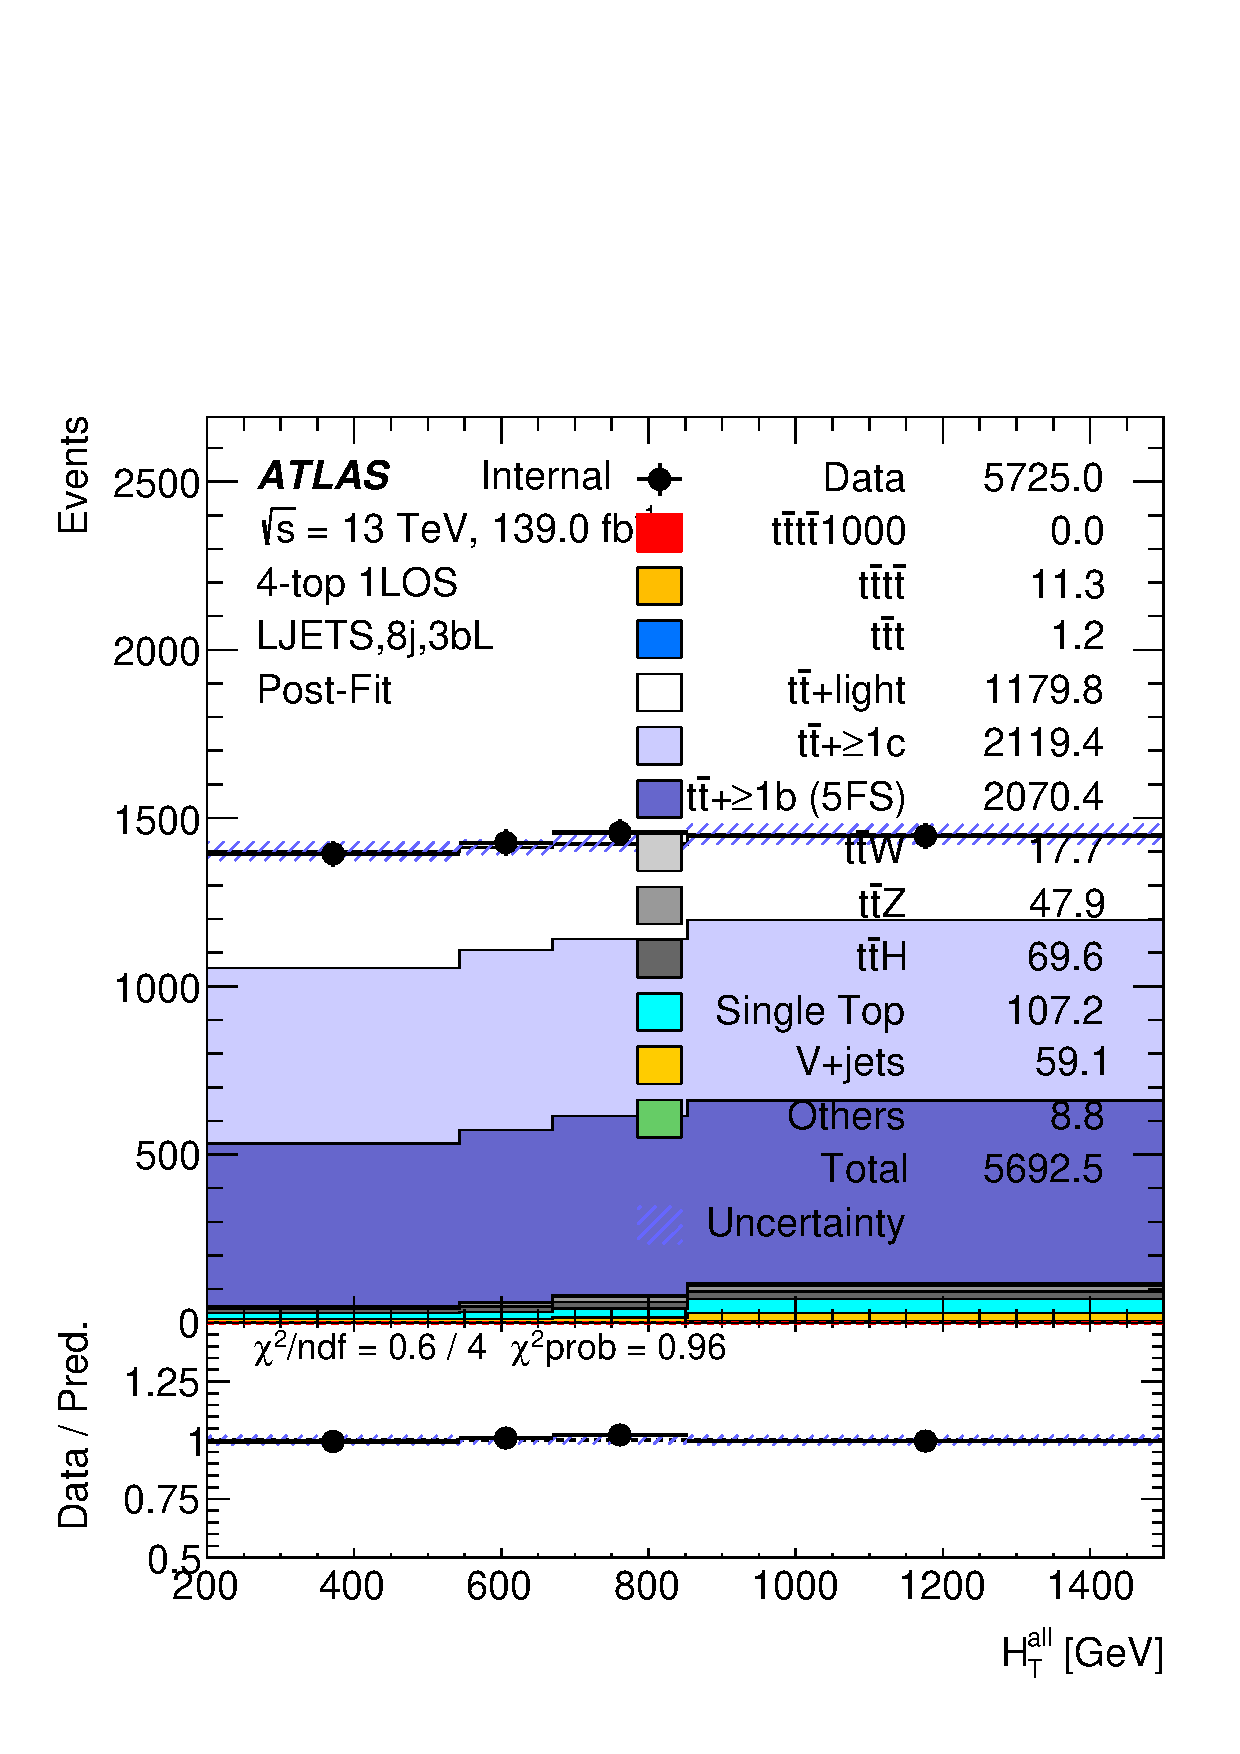
\includegraphics[width=0.23 \textwidth]{figures/fits/GNN/1000/all/data_unblindedBonly/Plots/ljets_8j3bL_postFit.pdf} &
        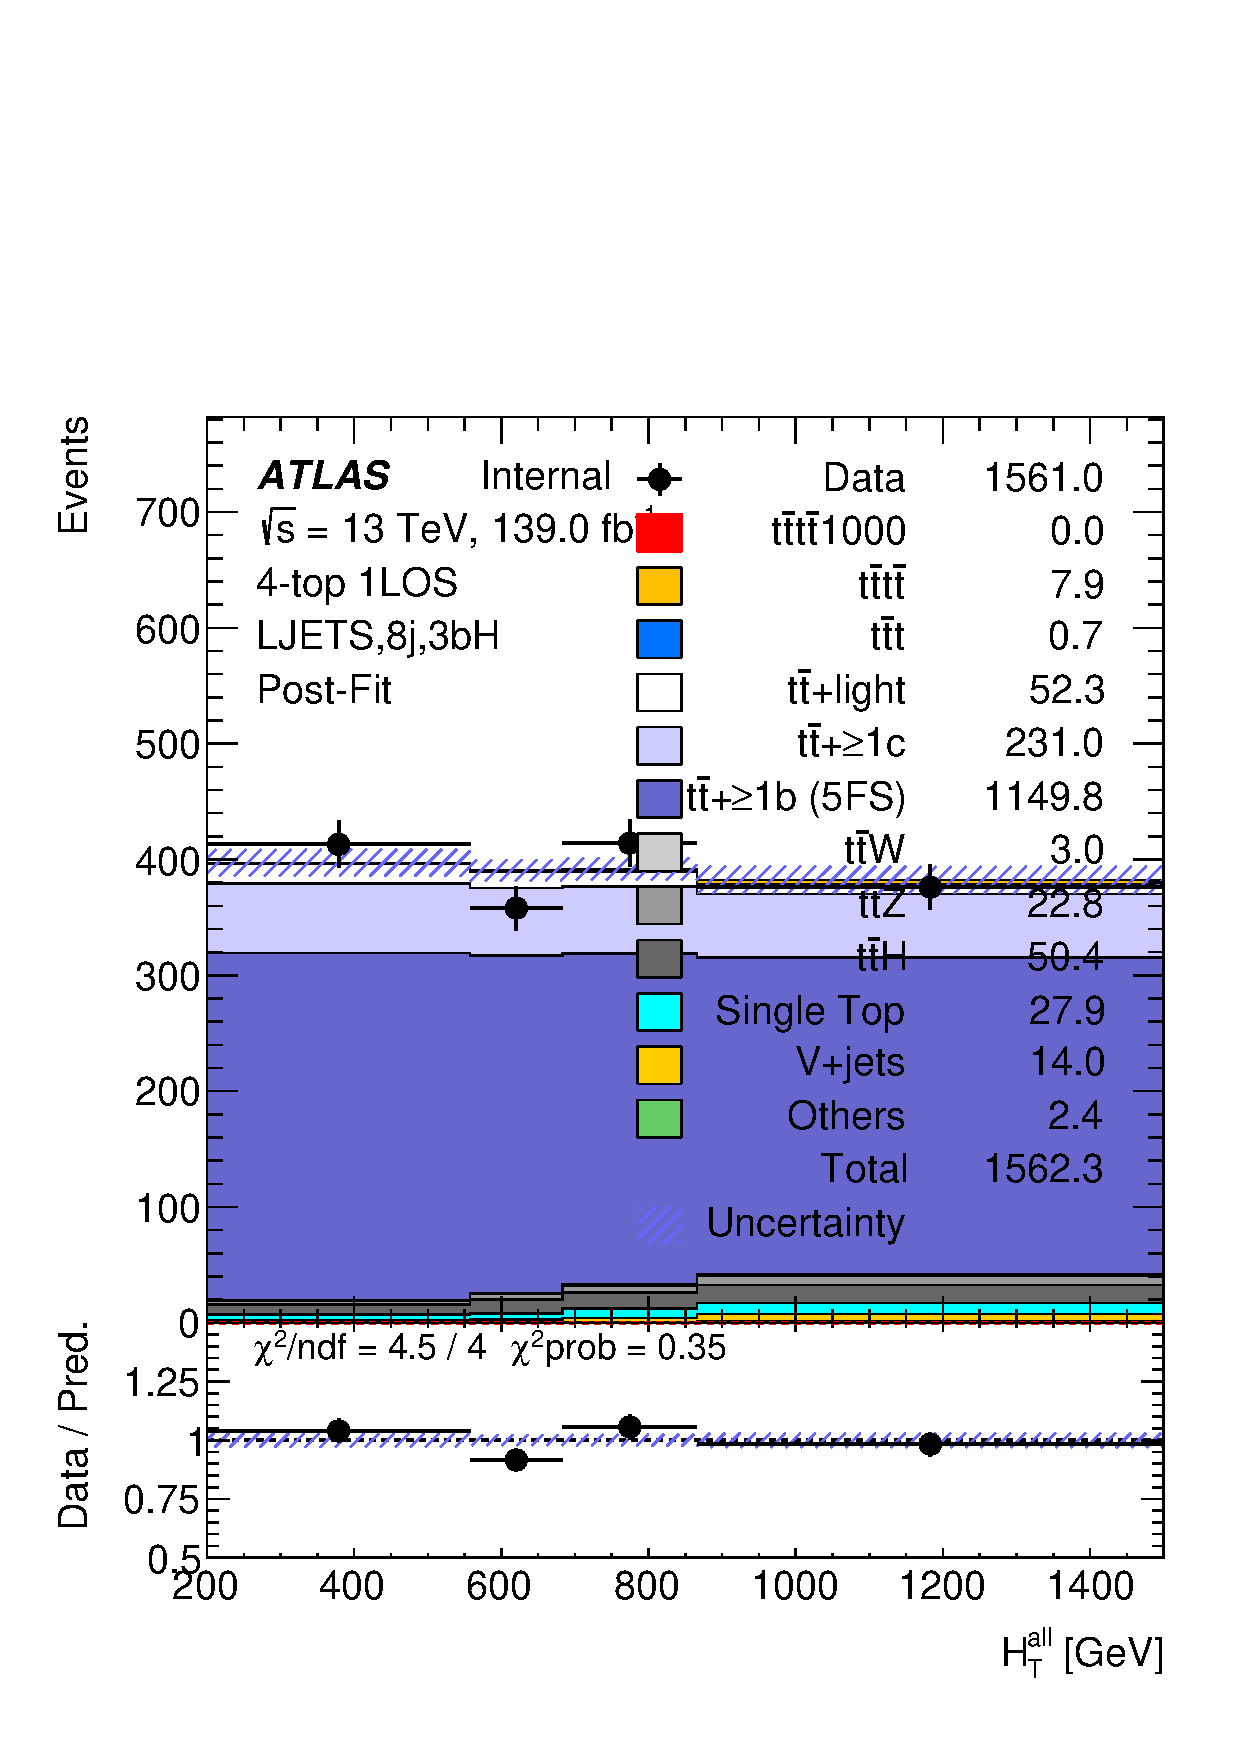
\includegraphics[width=0.23 \textwidth]{figures/fits/GNN/1000/all/data_unblindedBonly/Plots/ljets_8j3bH_postFit.pdf} &
        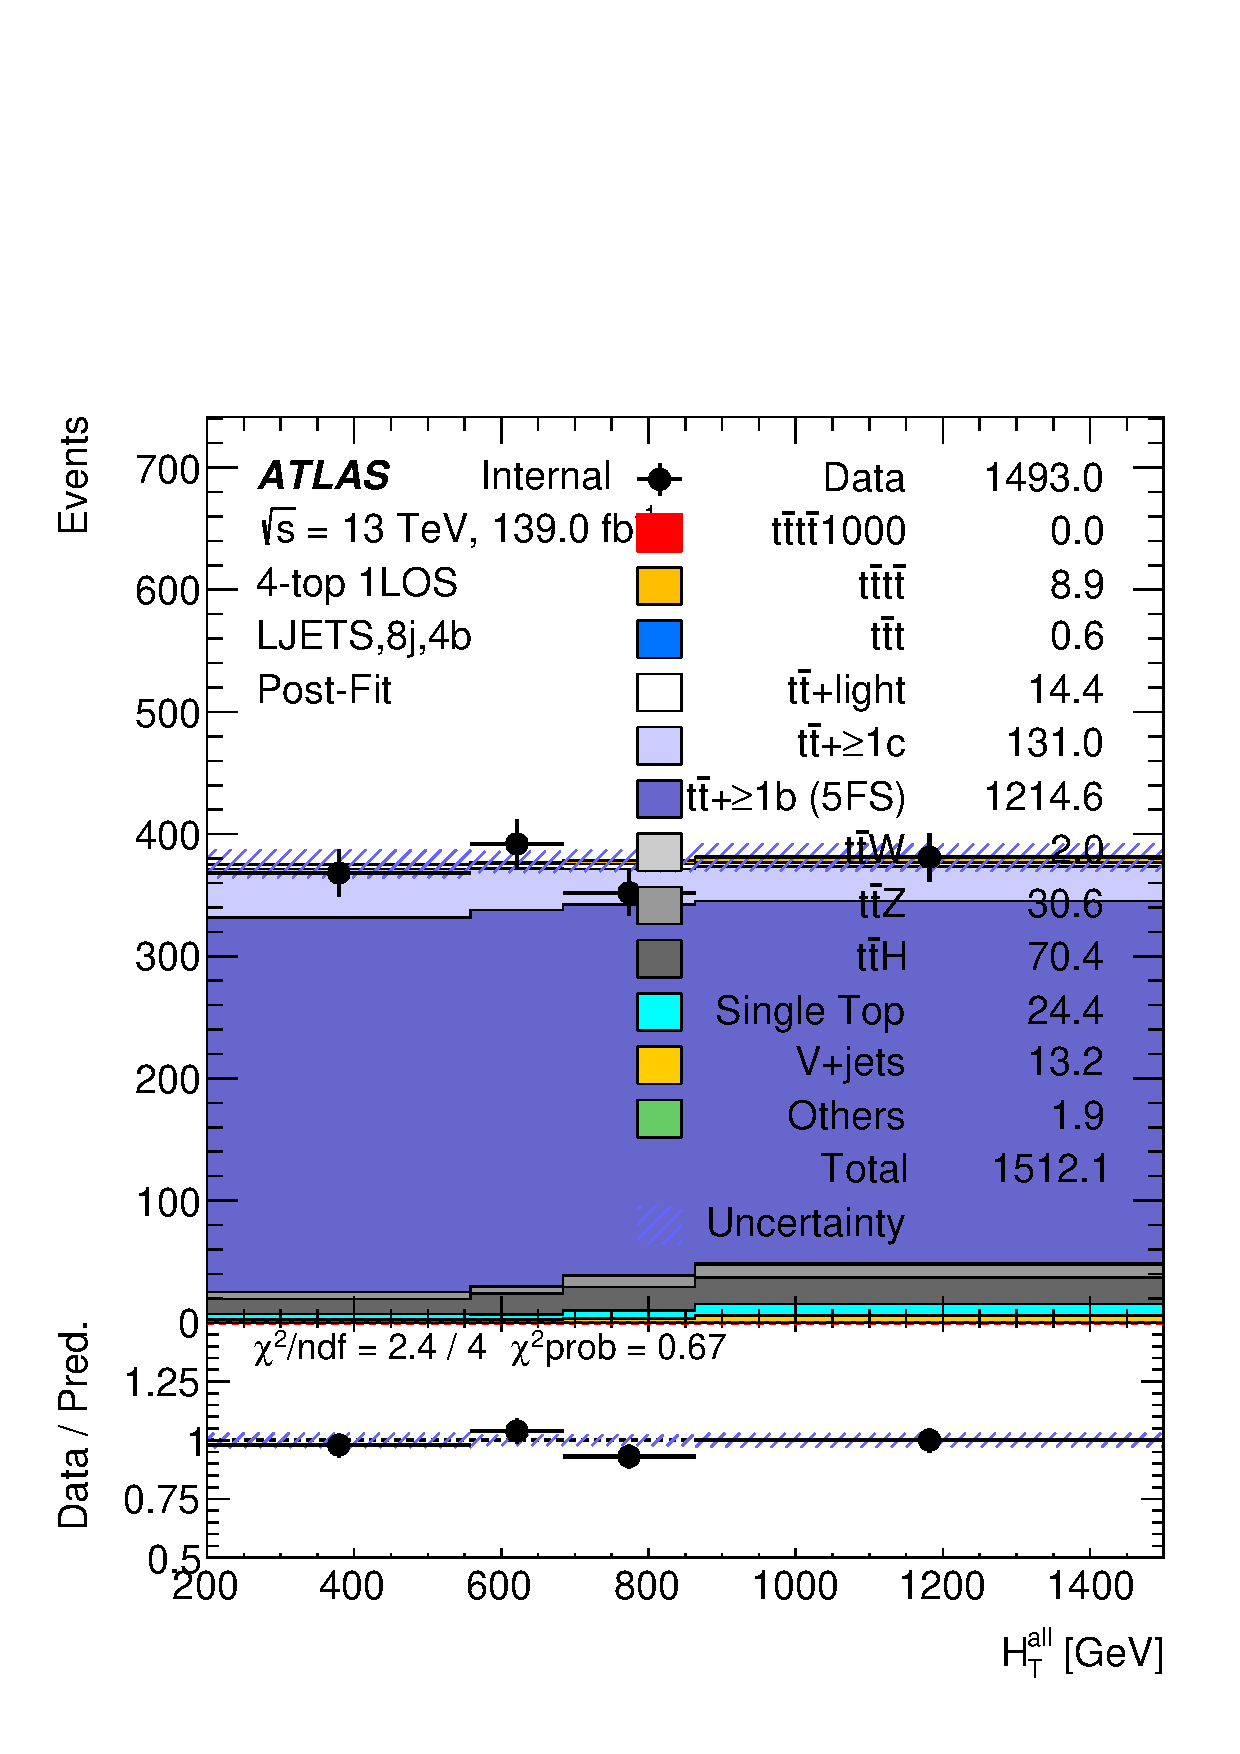
\includegraphics[width=0.23 \textwidth]{figures/fits/GNN/1000/all/data_unblindedBonly/Plots/ljets_8j4b_postFit.pdf} &
        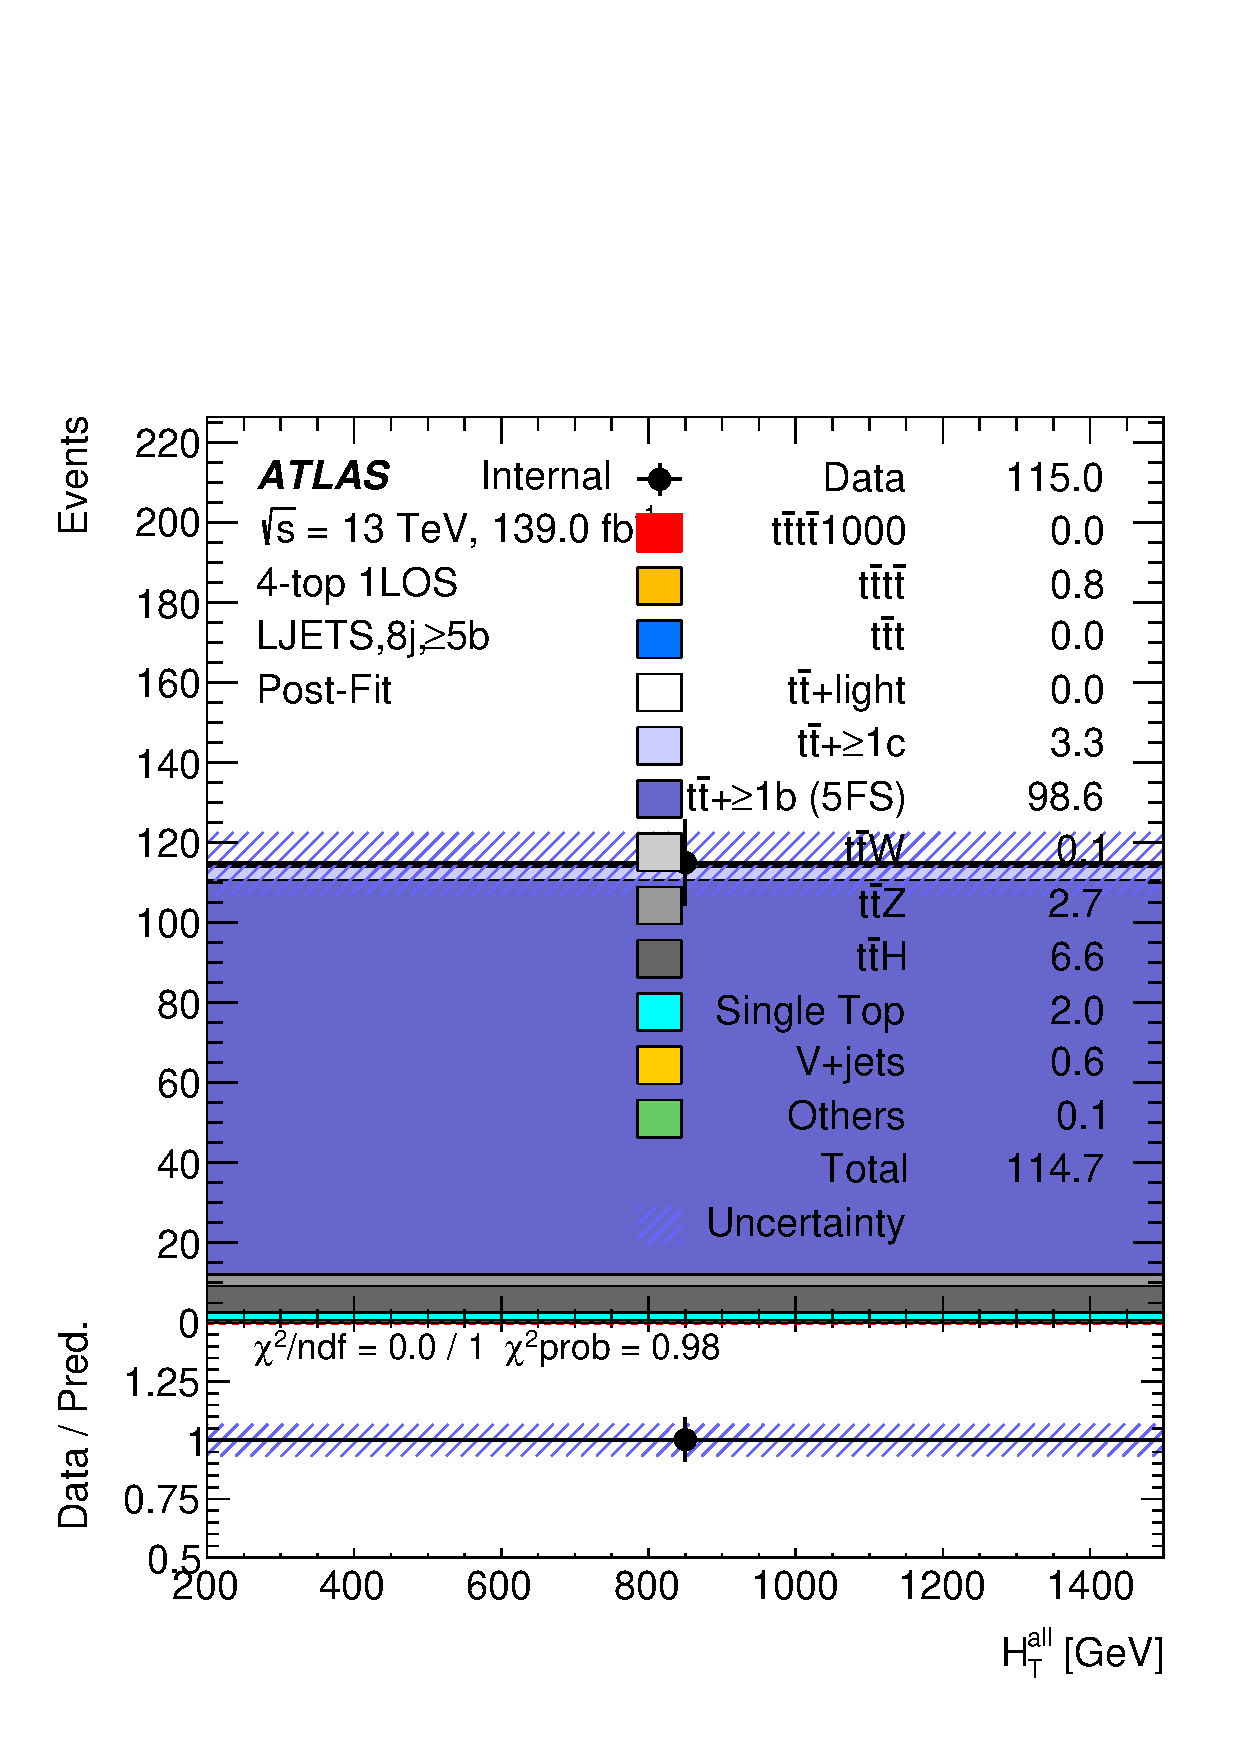
\includegraphics[width=0.23 \textwidth]{figures/fits/GNN/1000/all/data_unblindedBonly/Plots/ljets_8jge5b_postFit.pdf}\\

        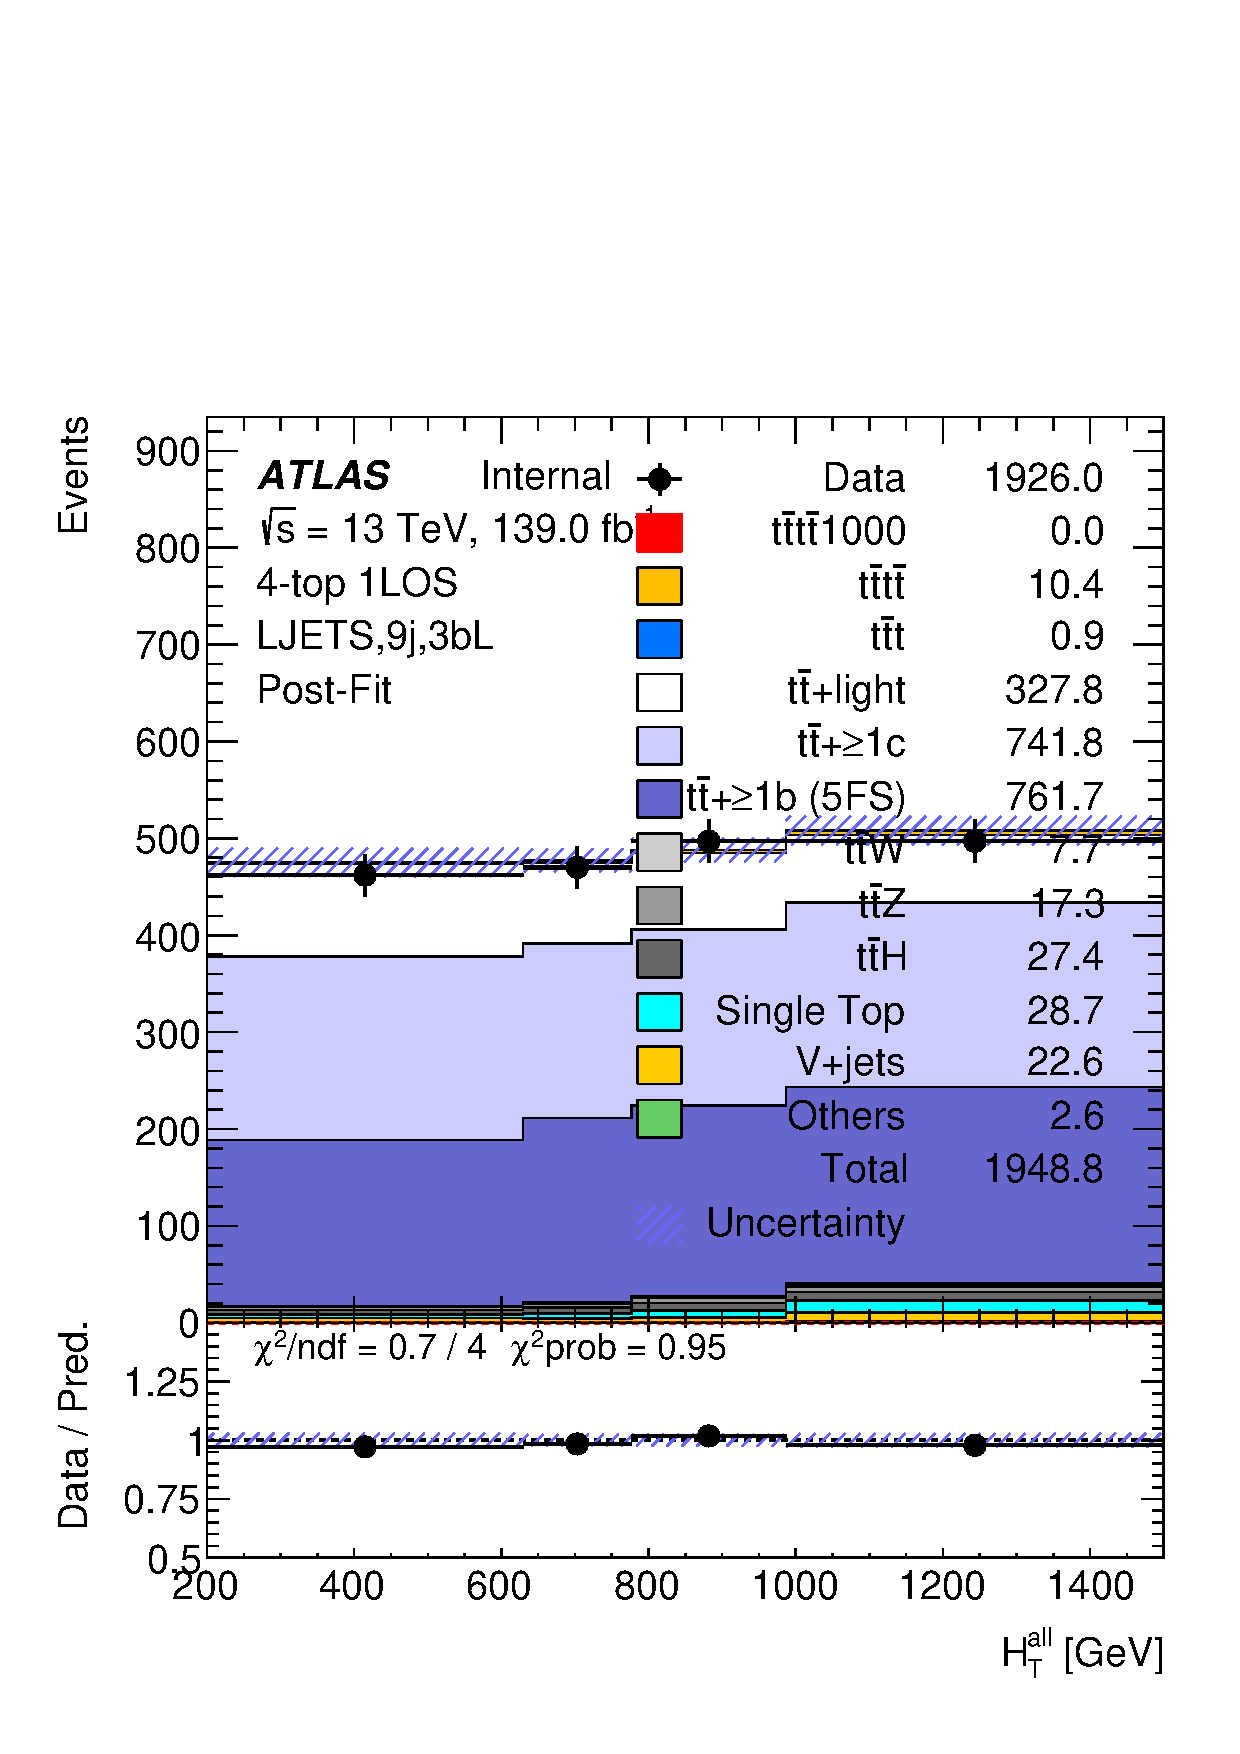
\includegraphics[width=0.23 \textwidth]{figures/fits/GNN/1000/all/data_unblindedBonly/Plots/ljets_9j3bL_postFit.pdf} &
        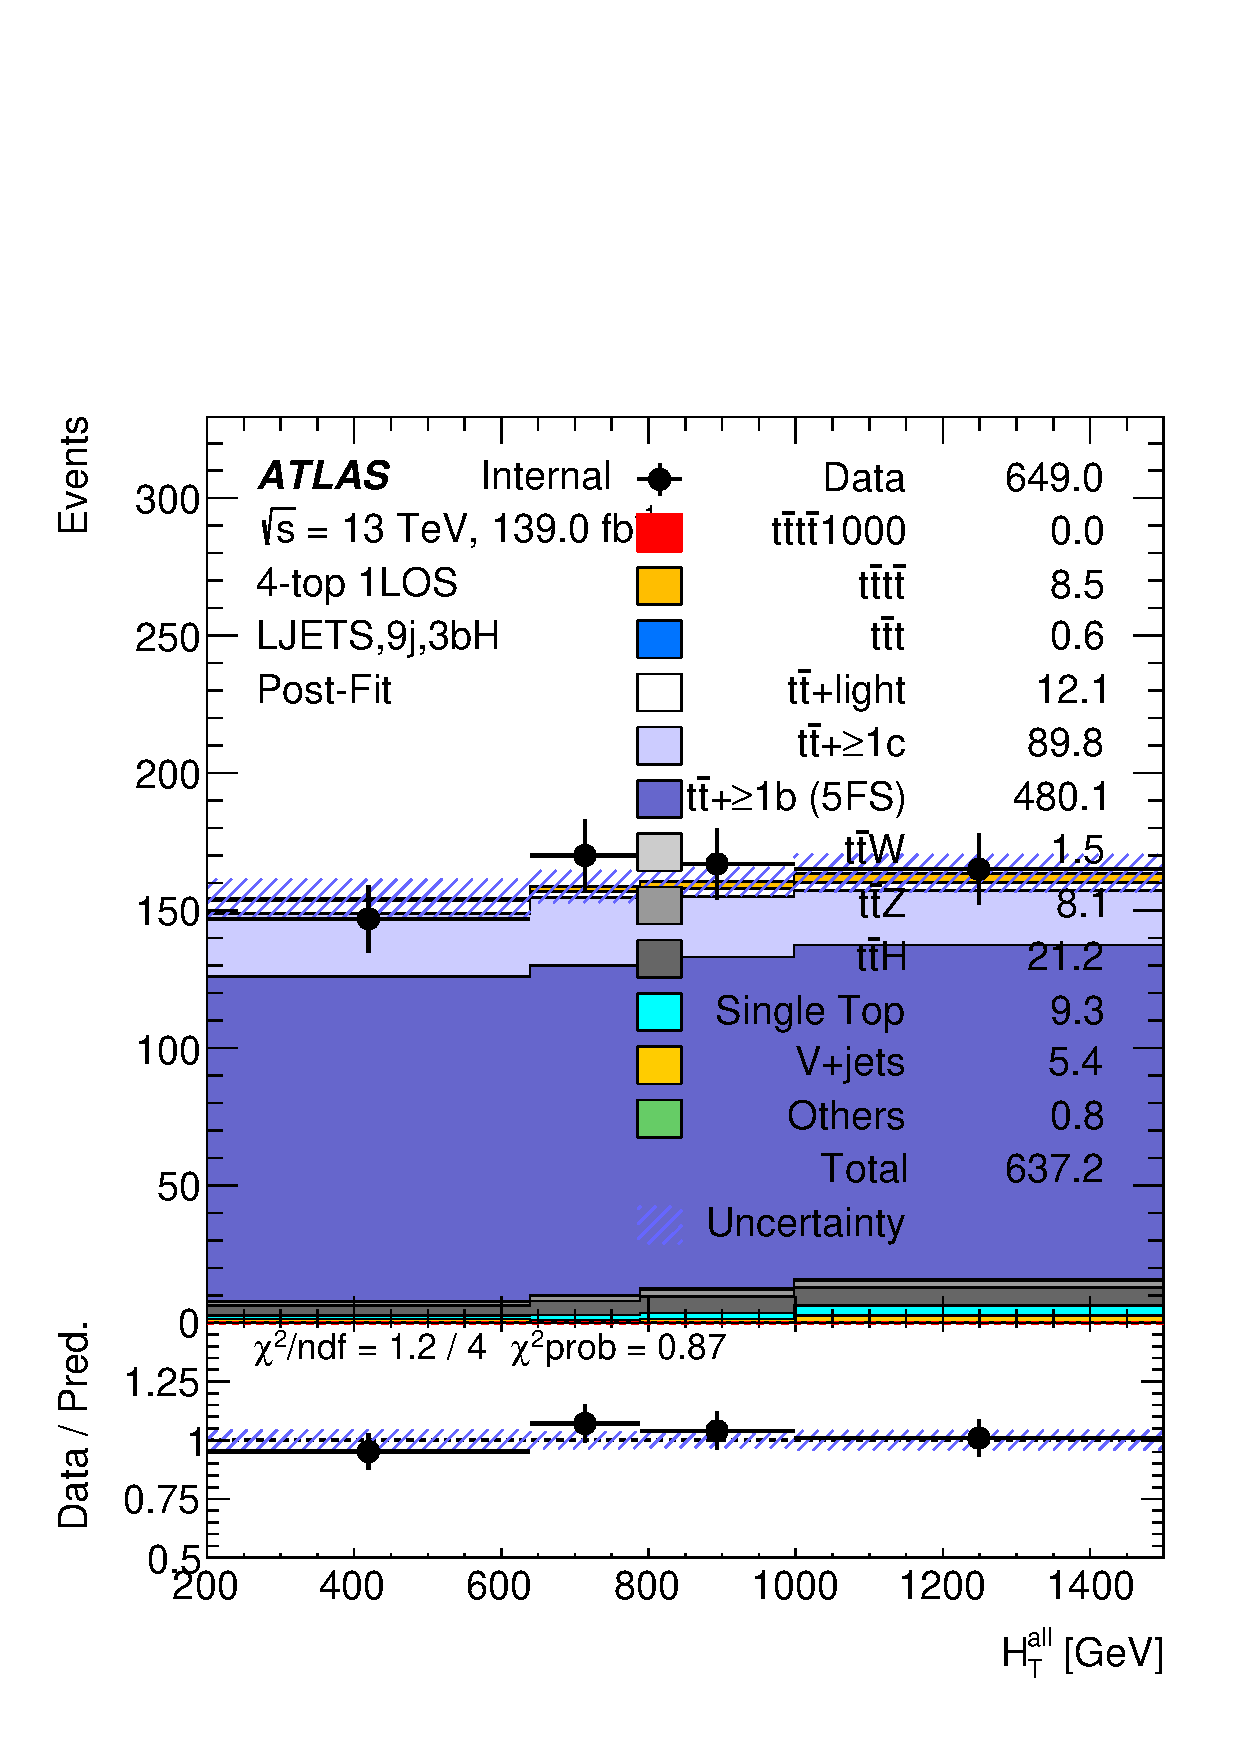
\includegraphics[width=0.23 \textwidth]{figures/fits/GNN/1000/all/data_unblindedBonly/Plots/ljets_9j3bH_postFit.pdf} &
        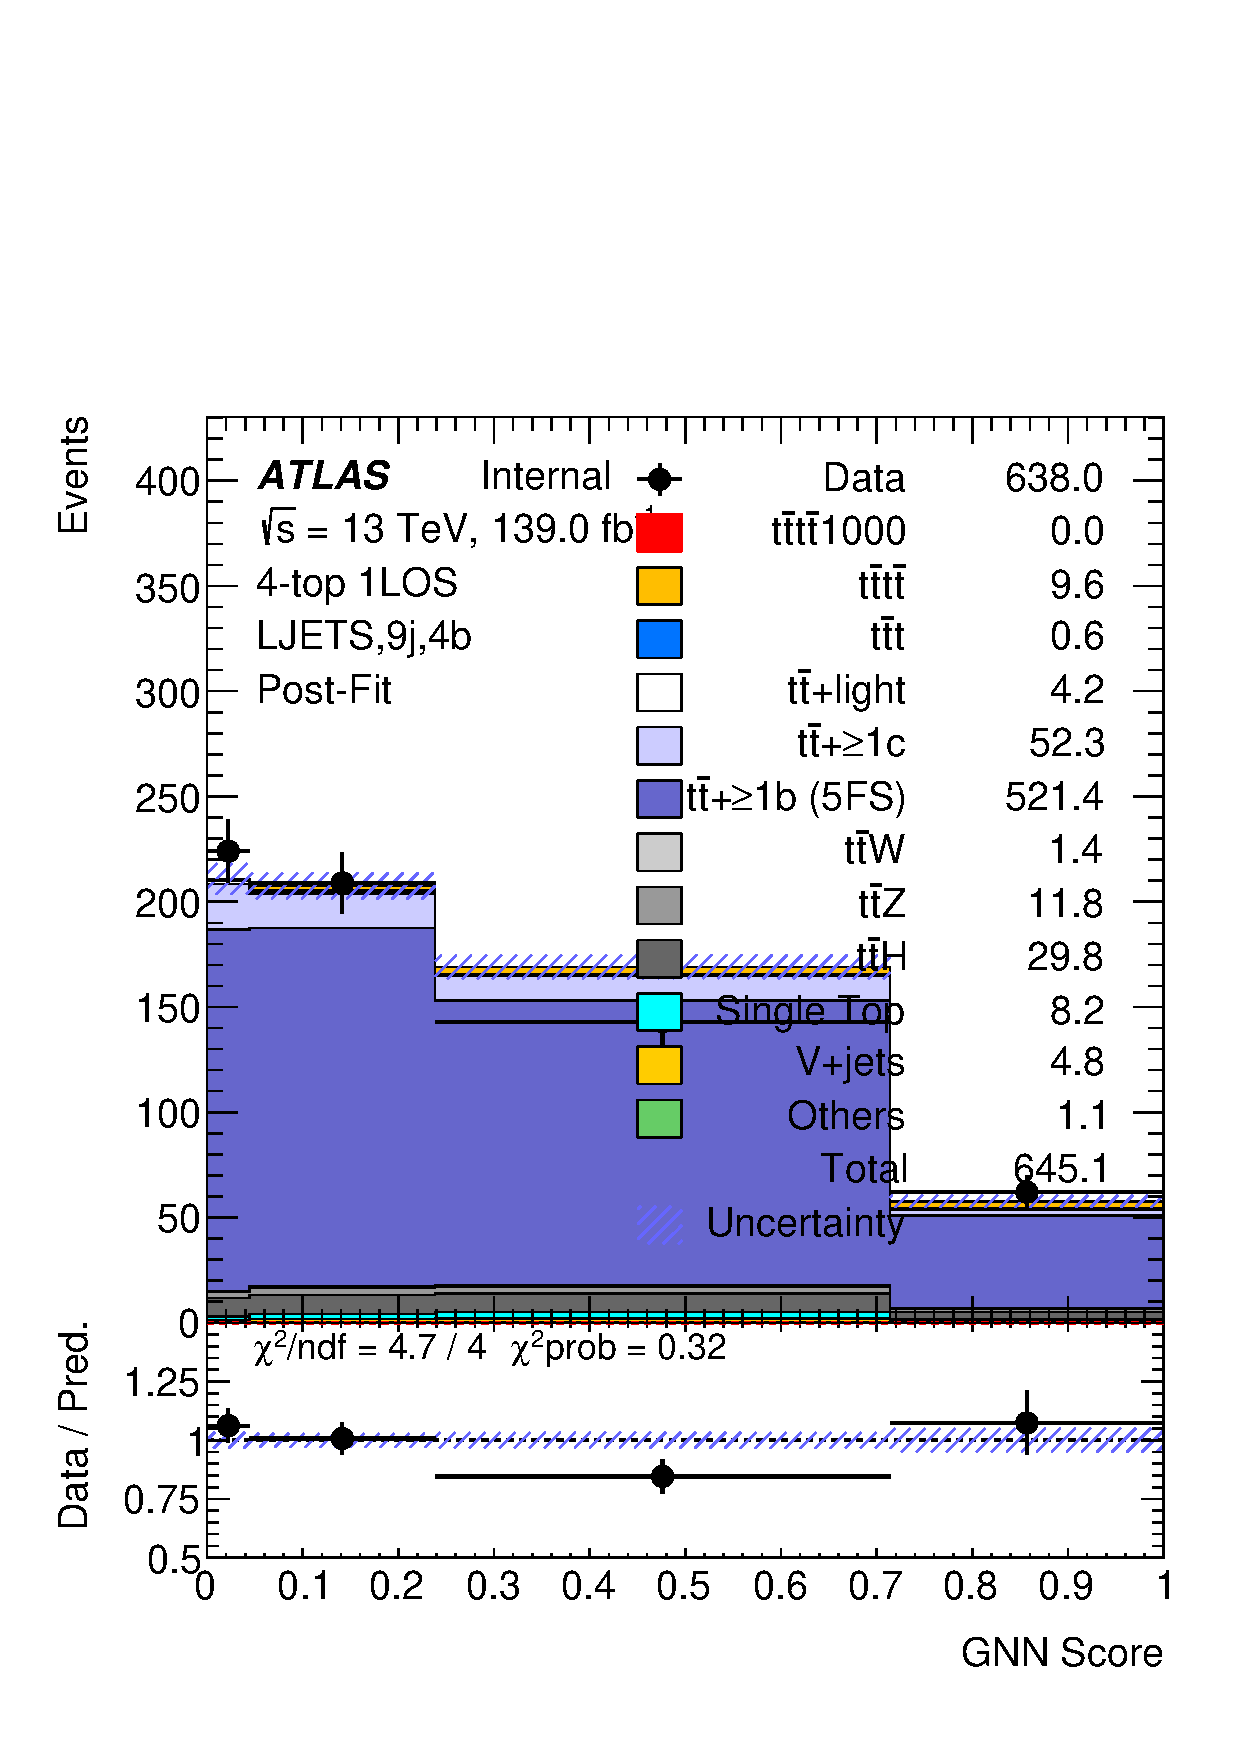
\includegraphics[width=0.23 \textwidth]{figures/fits/GNN/1000/all/data_unblindedBonly/Plots/ljets_9j4b_postFit.pdf} &
        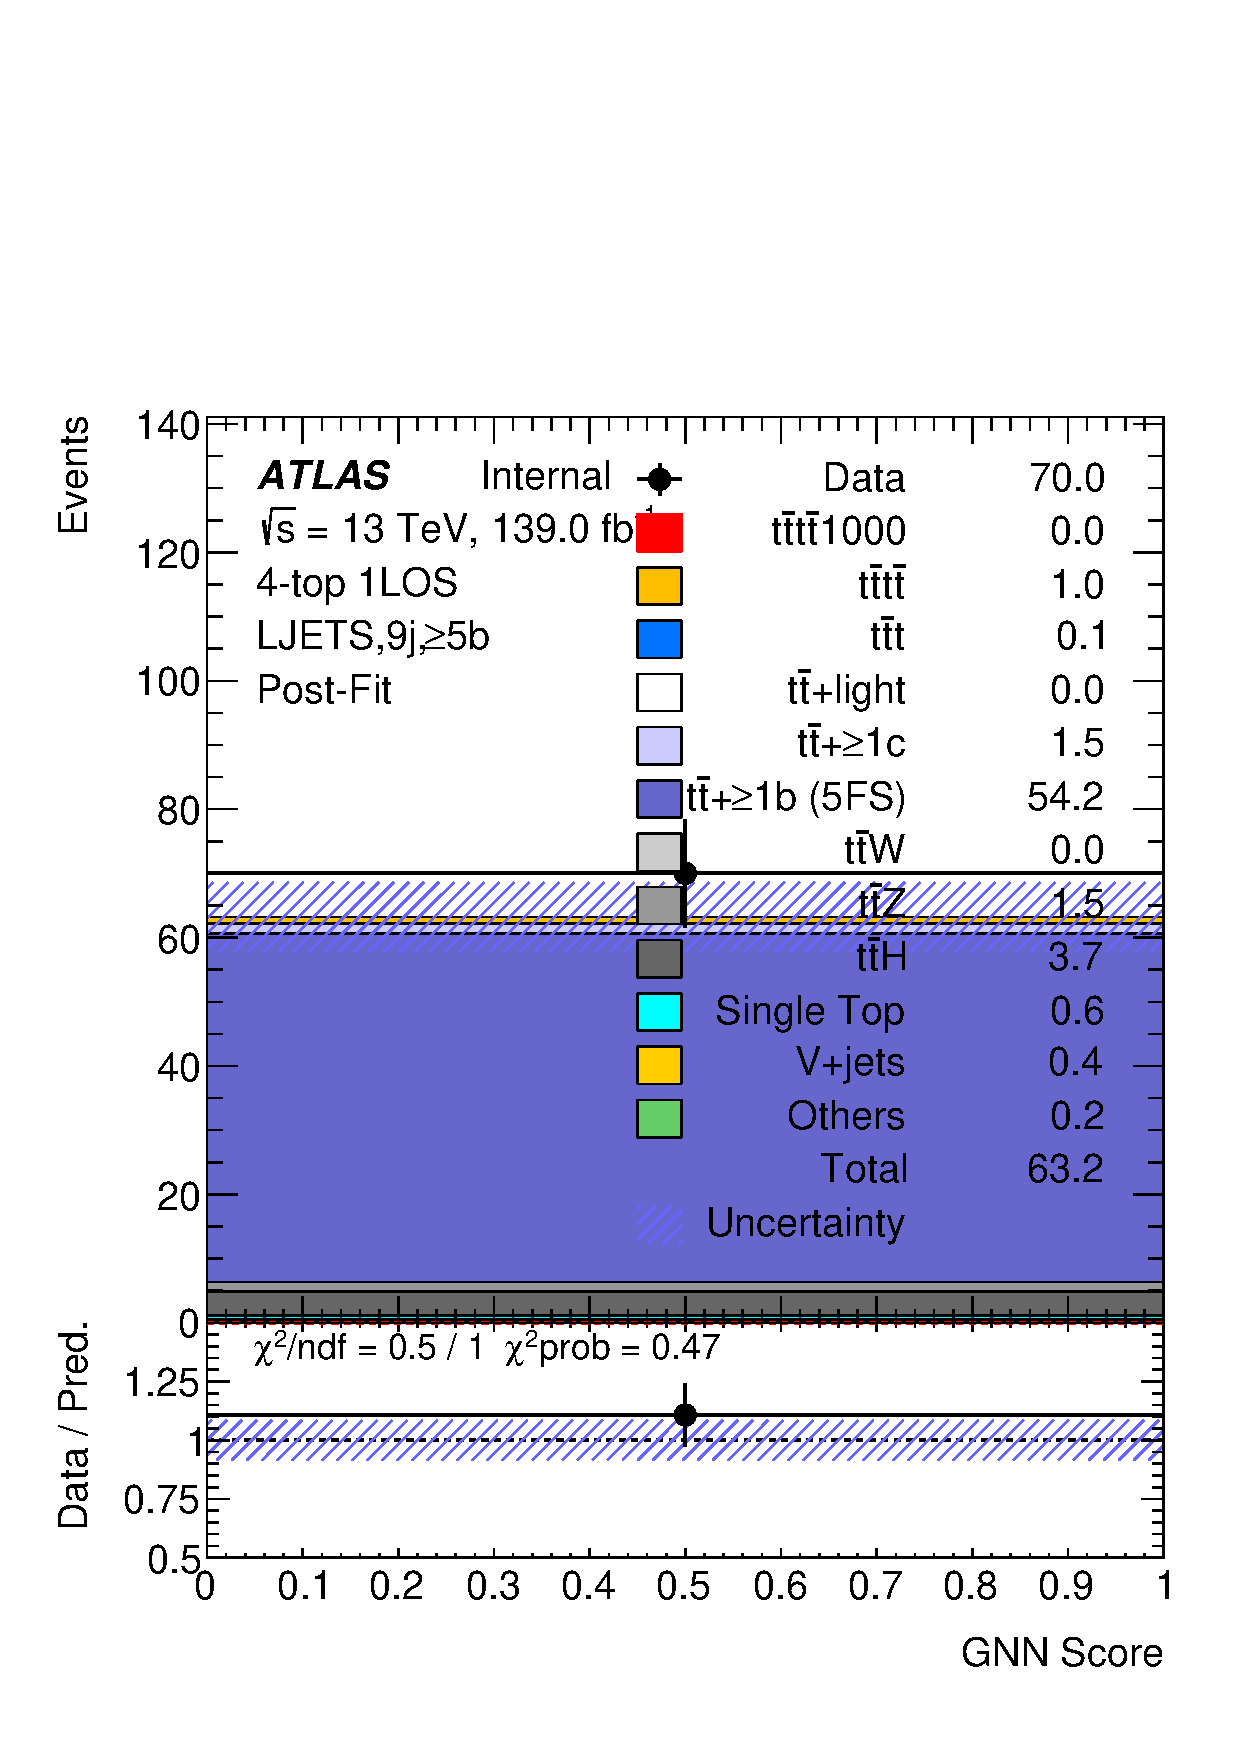
\includegraphics[width=0.23 \textwidth]{figures/fits/GNN/1000/all/data_unblindedBonly/Plots/ljets_9jge5b_postFit.pdf} \\

        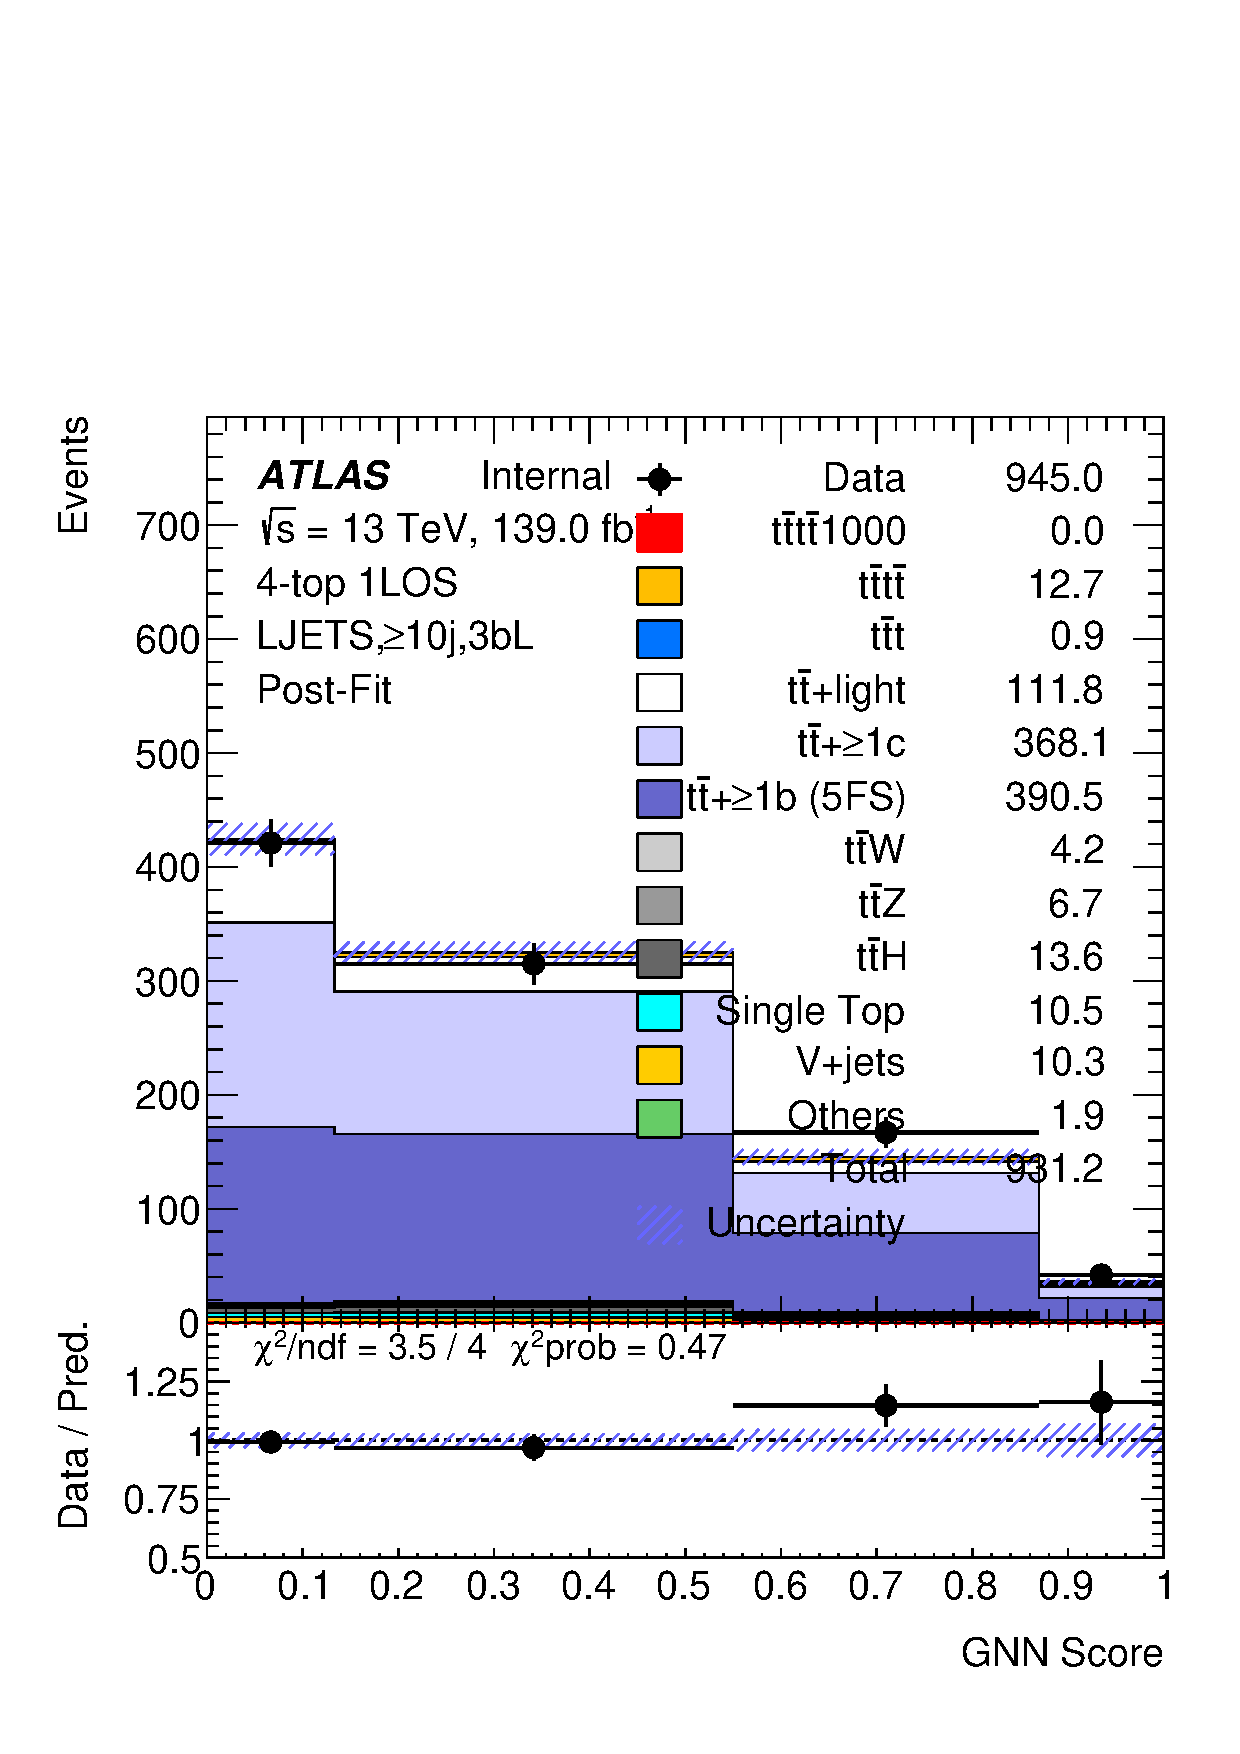
\includegraphics[width=0.23 \textwidth]{figures/fits/GNN/1000/all/data_unblindedBonly/Plots/ljets_ge10j3bL_postFit.pdf} &
        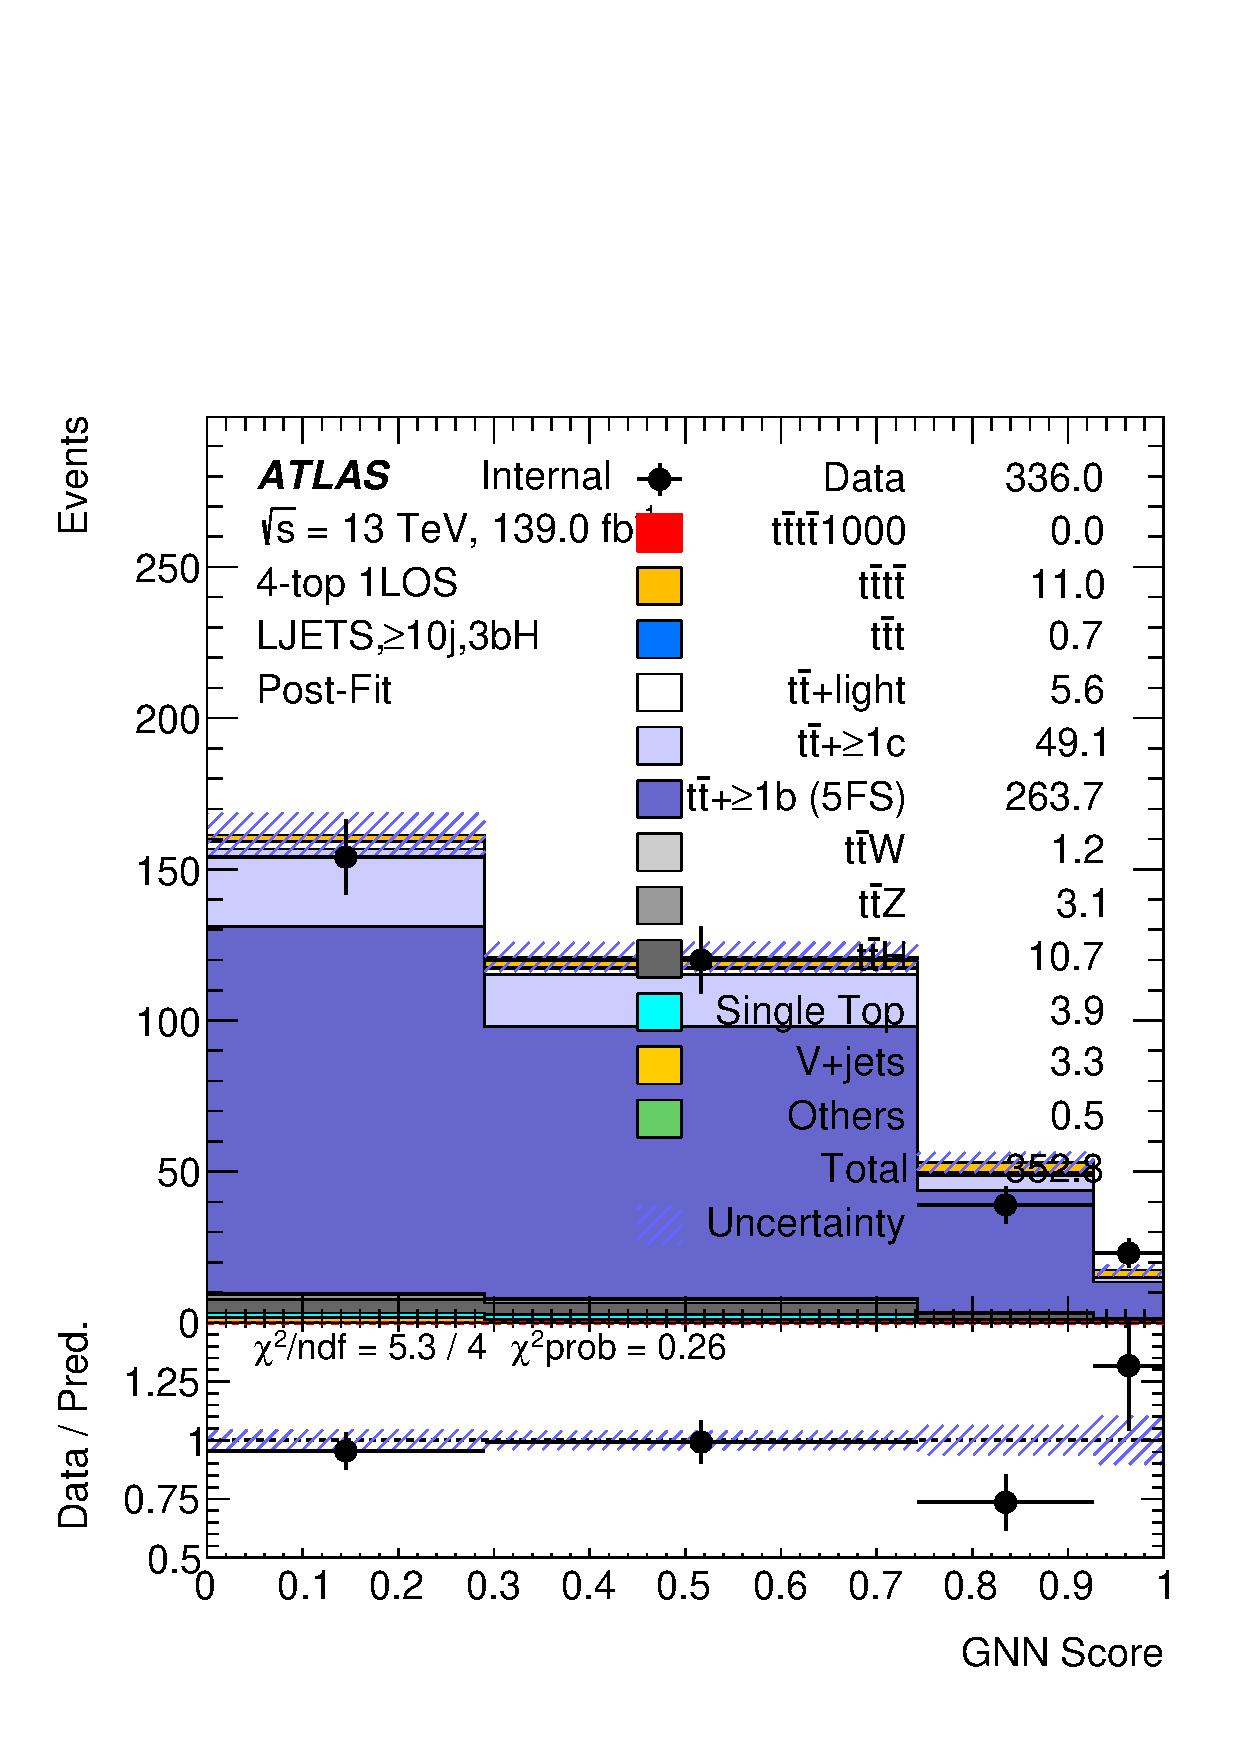
\includegraphics[width=0.23 \textwidth]{figures/fits/GNN/1000/all/data_unblindedBonly/Plots/ljets_ge10j3bH_postFit.pdf} &
        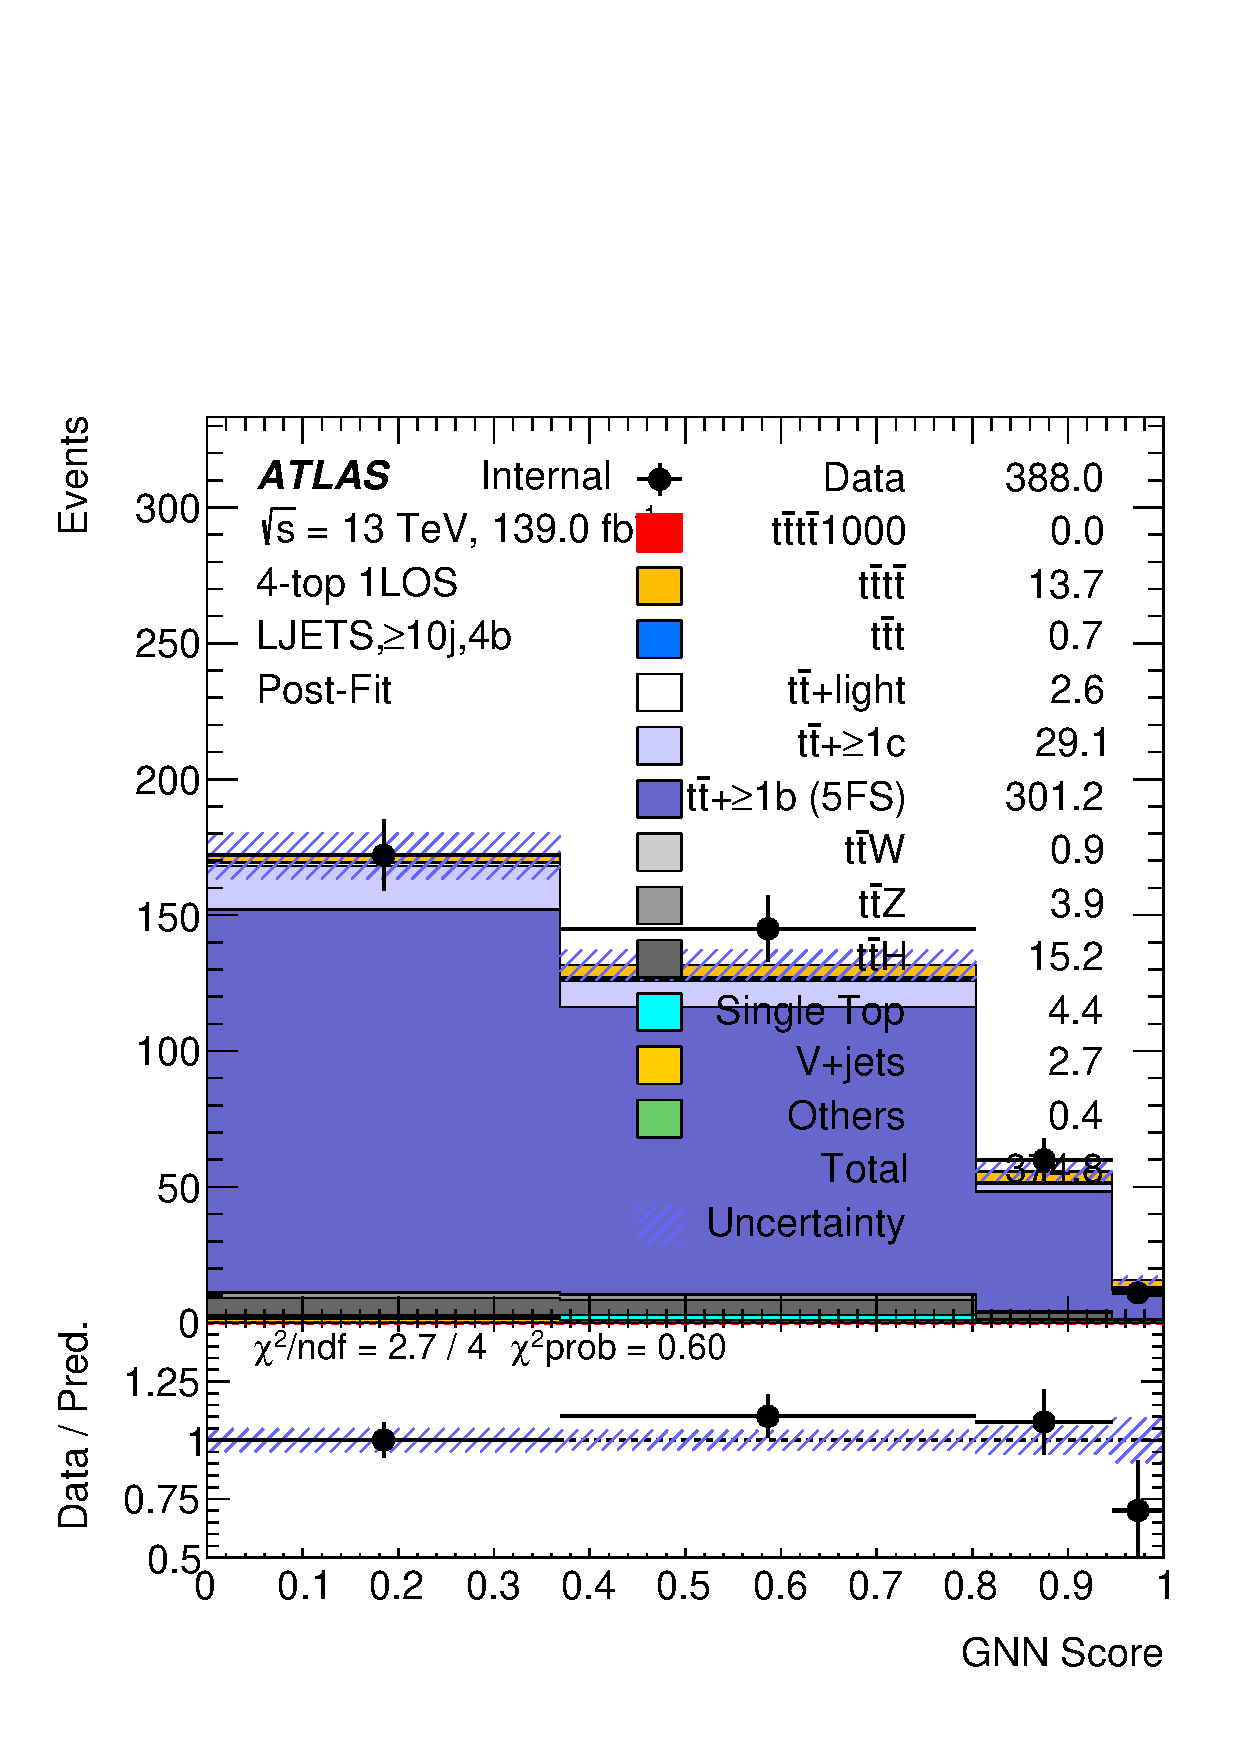
\includegraphics[width=0.23 \textwidth]{figures/fits/GNN/1000/all/data_unblindedBonly/Plots/ljets_ge10j4b_postFit.pdf} &
        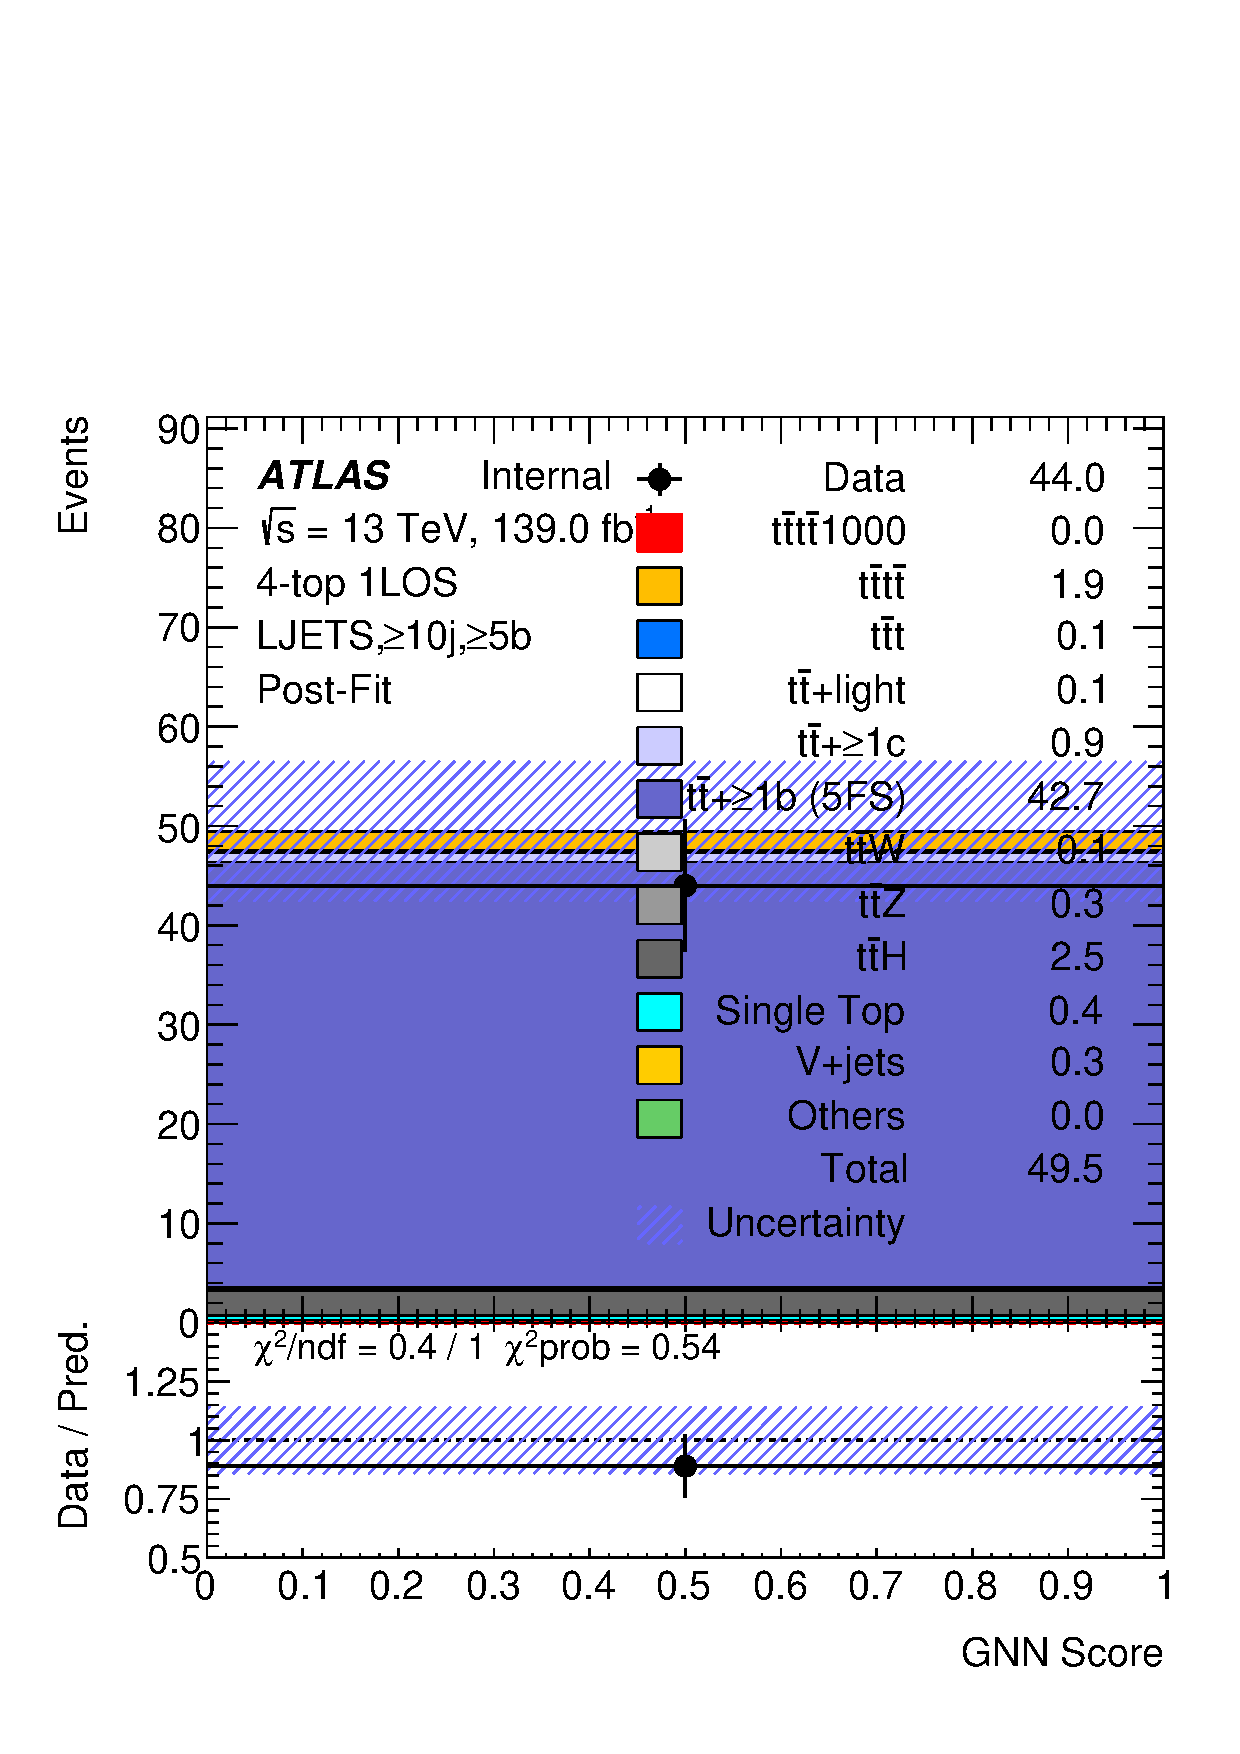
\includegraphics[width=0.23 \textwidth]{figures/fits/GNN/1000/all/data_unblindedBonly/Plots/ljets_ge10jge5b_postFit.pdf} \\
        \end{tabular}
        \caption{\label{fig:Postfit_Yields_1L_1000GeV}Post-fit distributions for 1L regions associated with different signal and background samples, compared with data yields for mH = 1000 GeV. The fit is done using all regions (1L+2L). The same plots for mH = 400 GeV are shown in Figure \ref{fig:Postfit_Yields_1L}.}
\end{center}
\end{figure}

\begin{figure}[htbp!]
        \begin{center} \setlength{\tabcolsep}{2.5pt}\footnotesize
        \begin{tabular}{ccc}
        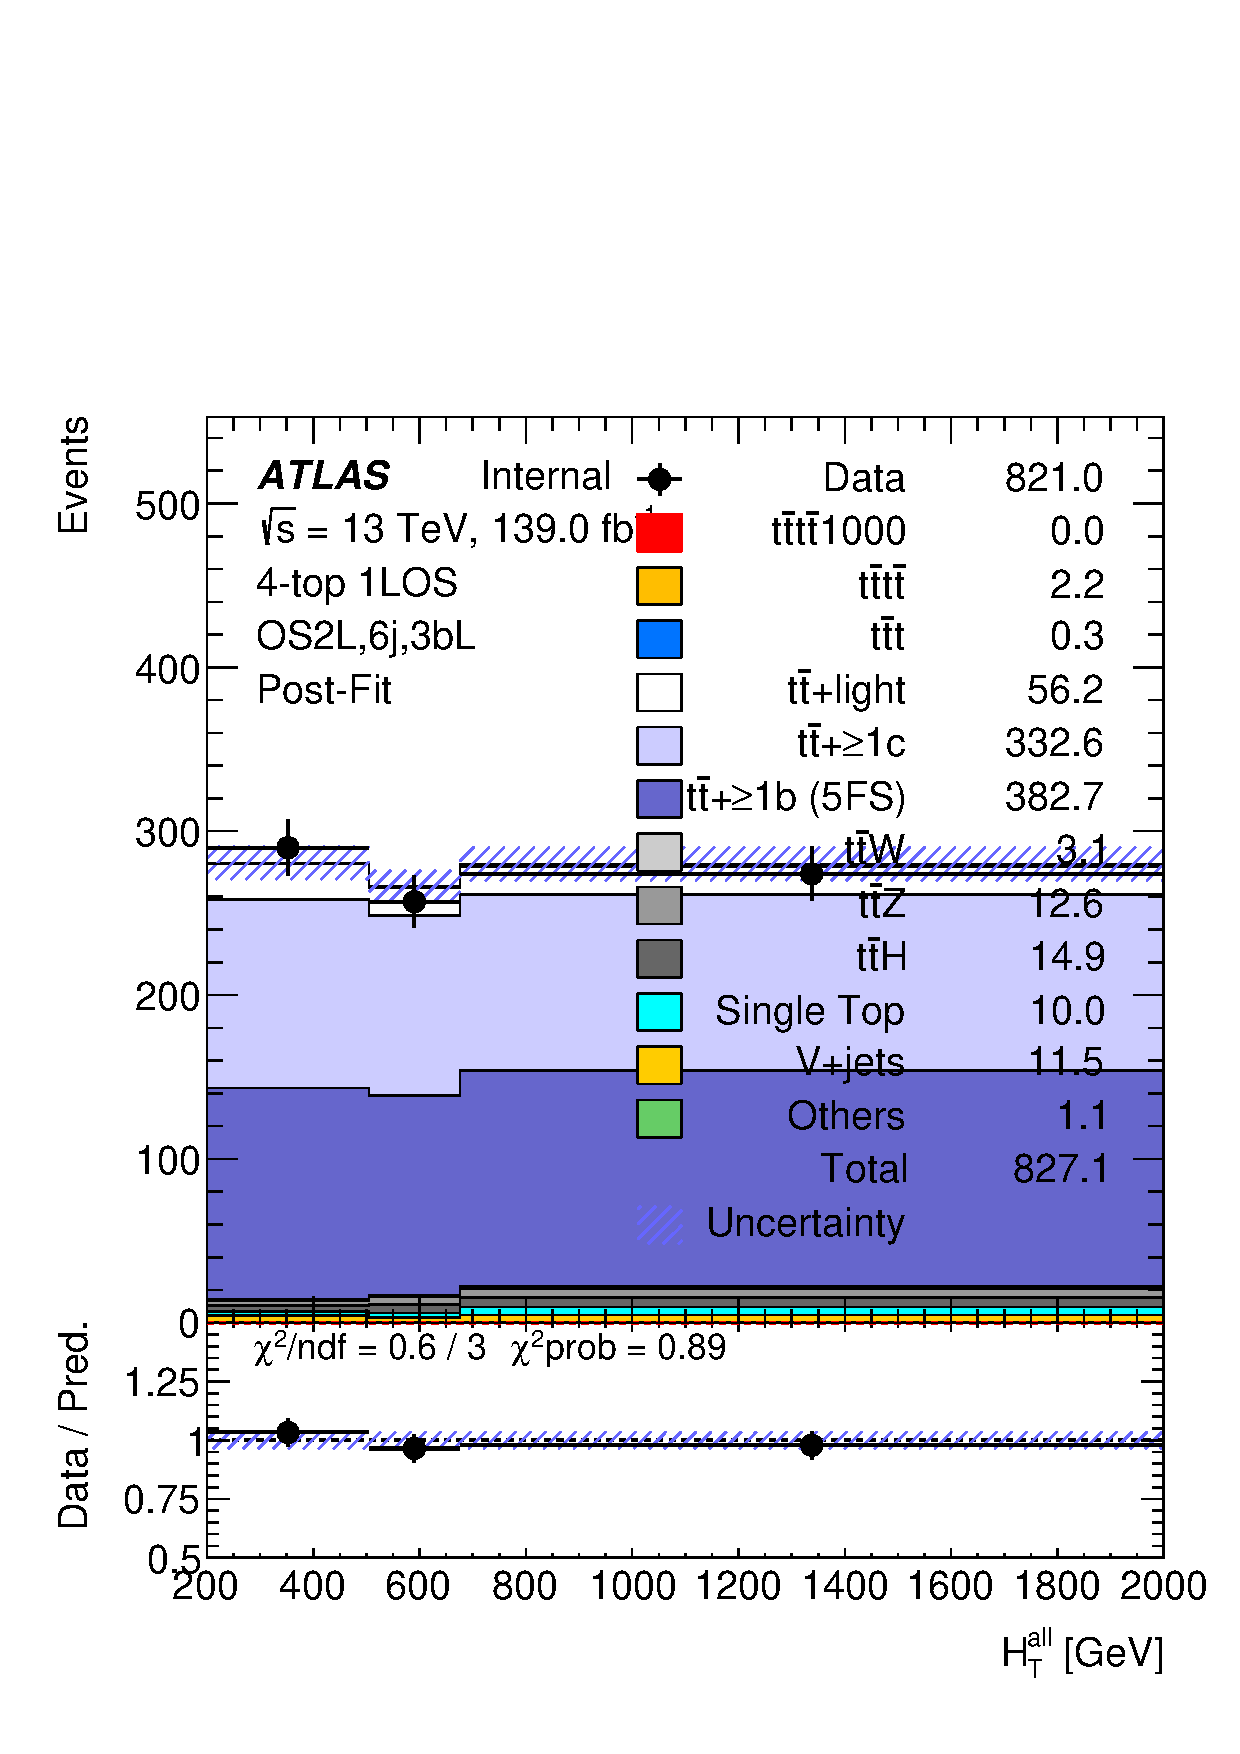
\includegraphics[width=0.31 \textwidth]{figures/fits/GNN/1000/all/data_unblindedBonly/Plots/os2l_6j3bL_postFit.pdf} &
        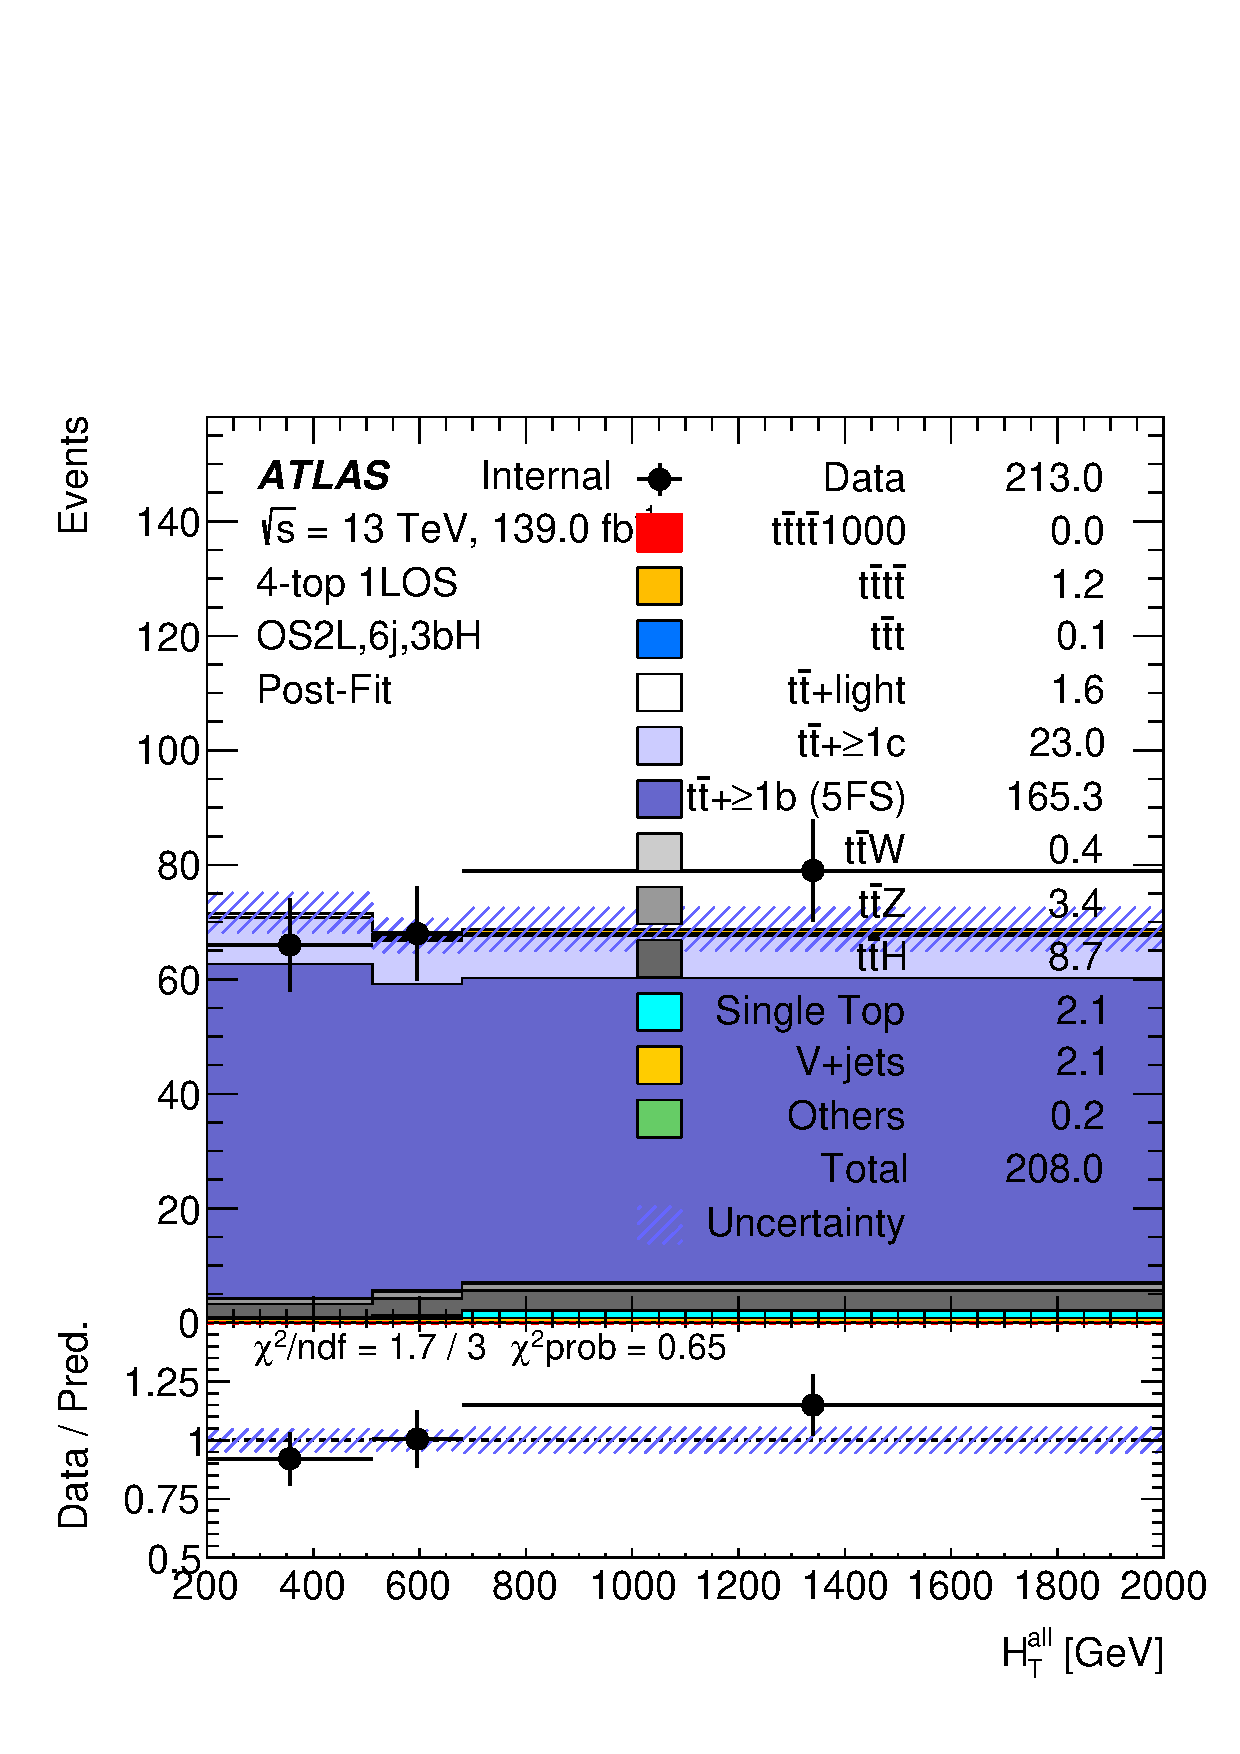
\includegraphics[width=0.31 \textwidth]{figures/fits/GNN/1000/all/data_unblindedBonly/Plots/os2l_6j3bH_postFit.pdf} &
        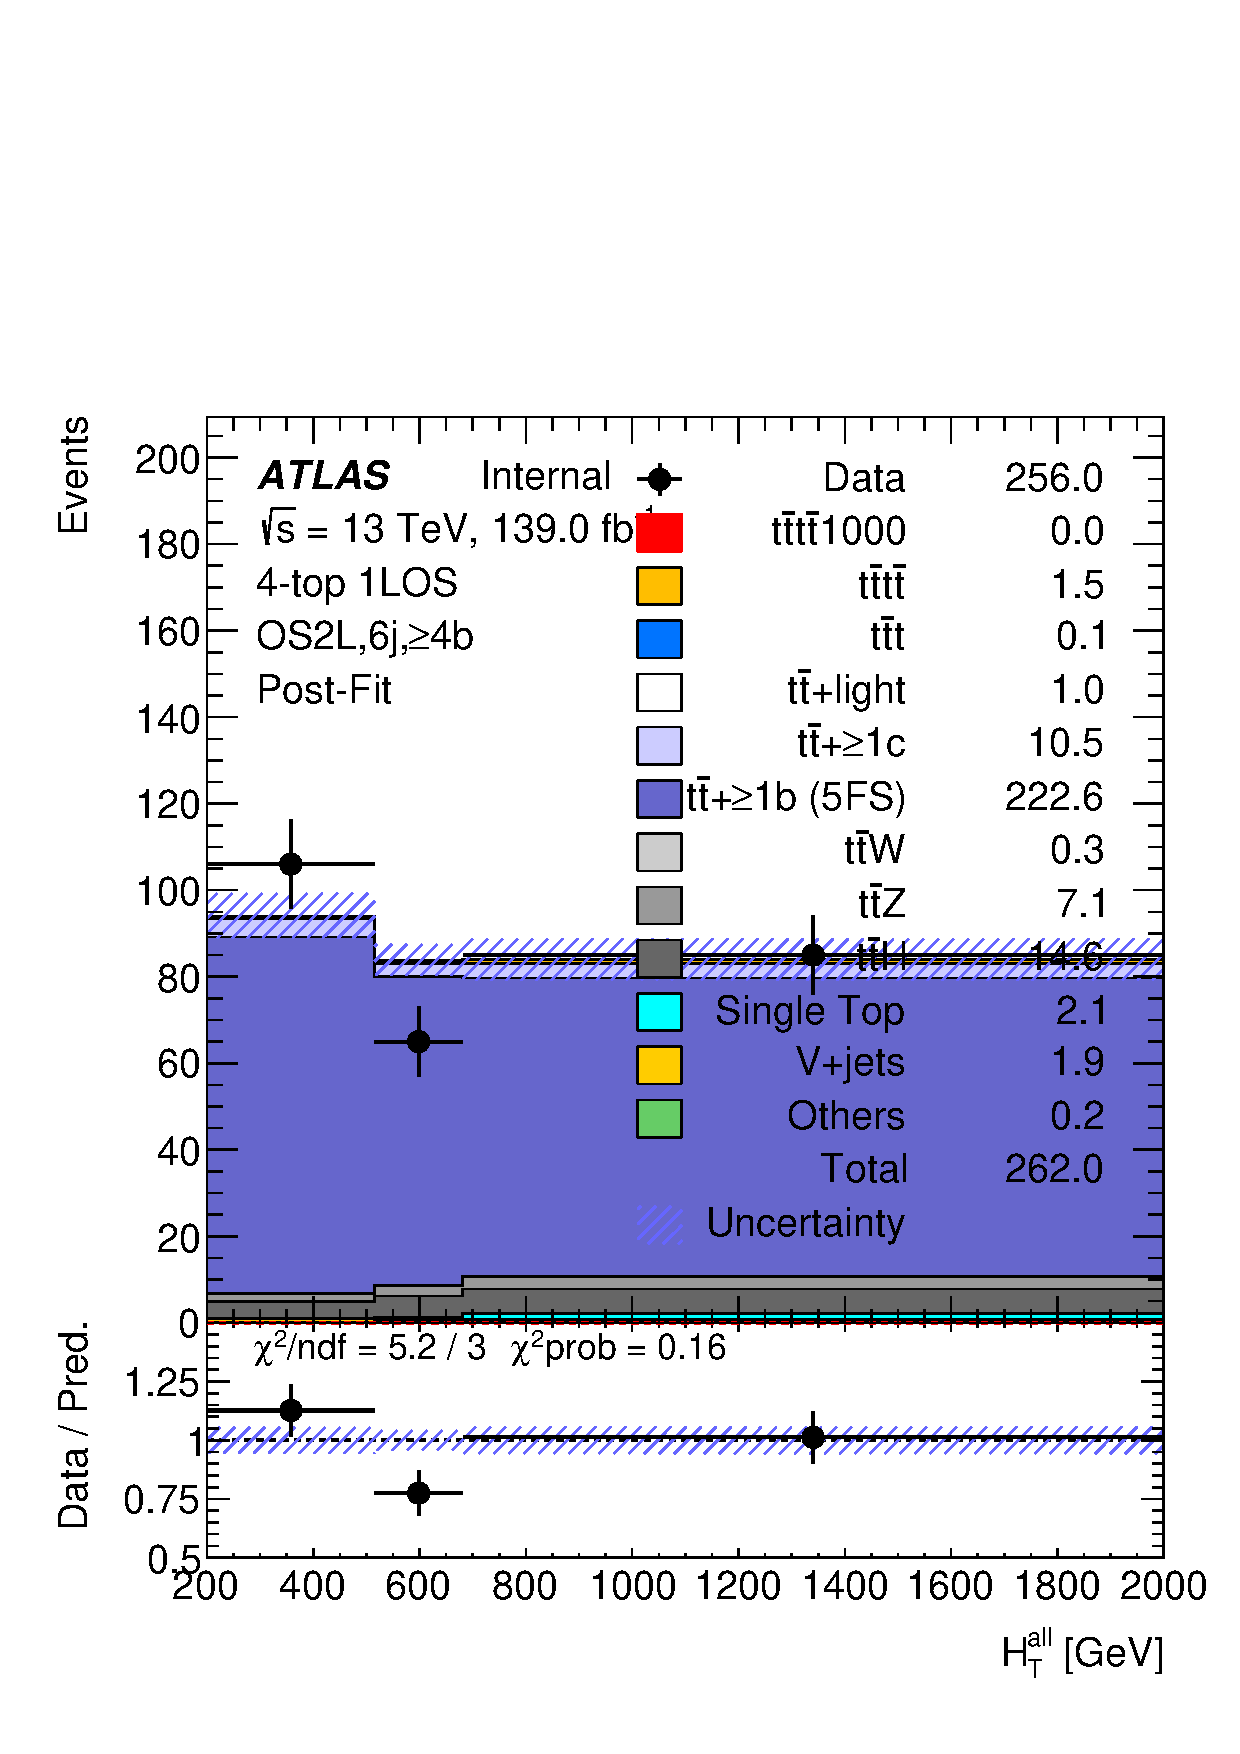
\includegraphics[width=0.31 \textwidth]{figures/fits/GNN/1000/all/data_unblindedBonly/Plots/os2l_6jge4b_postFit.pdf} \\

        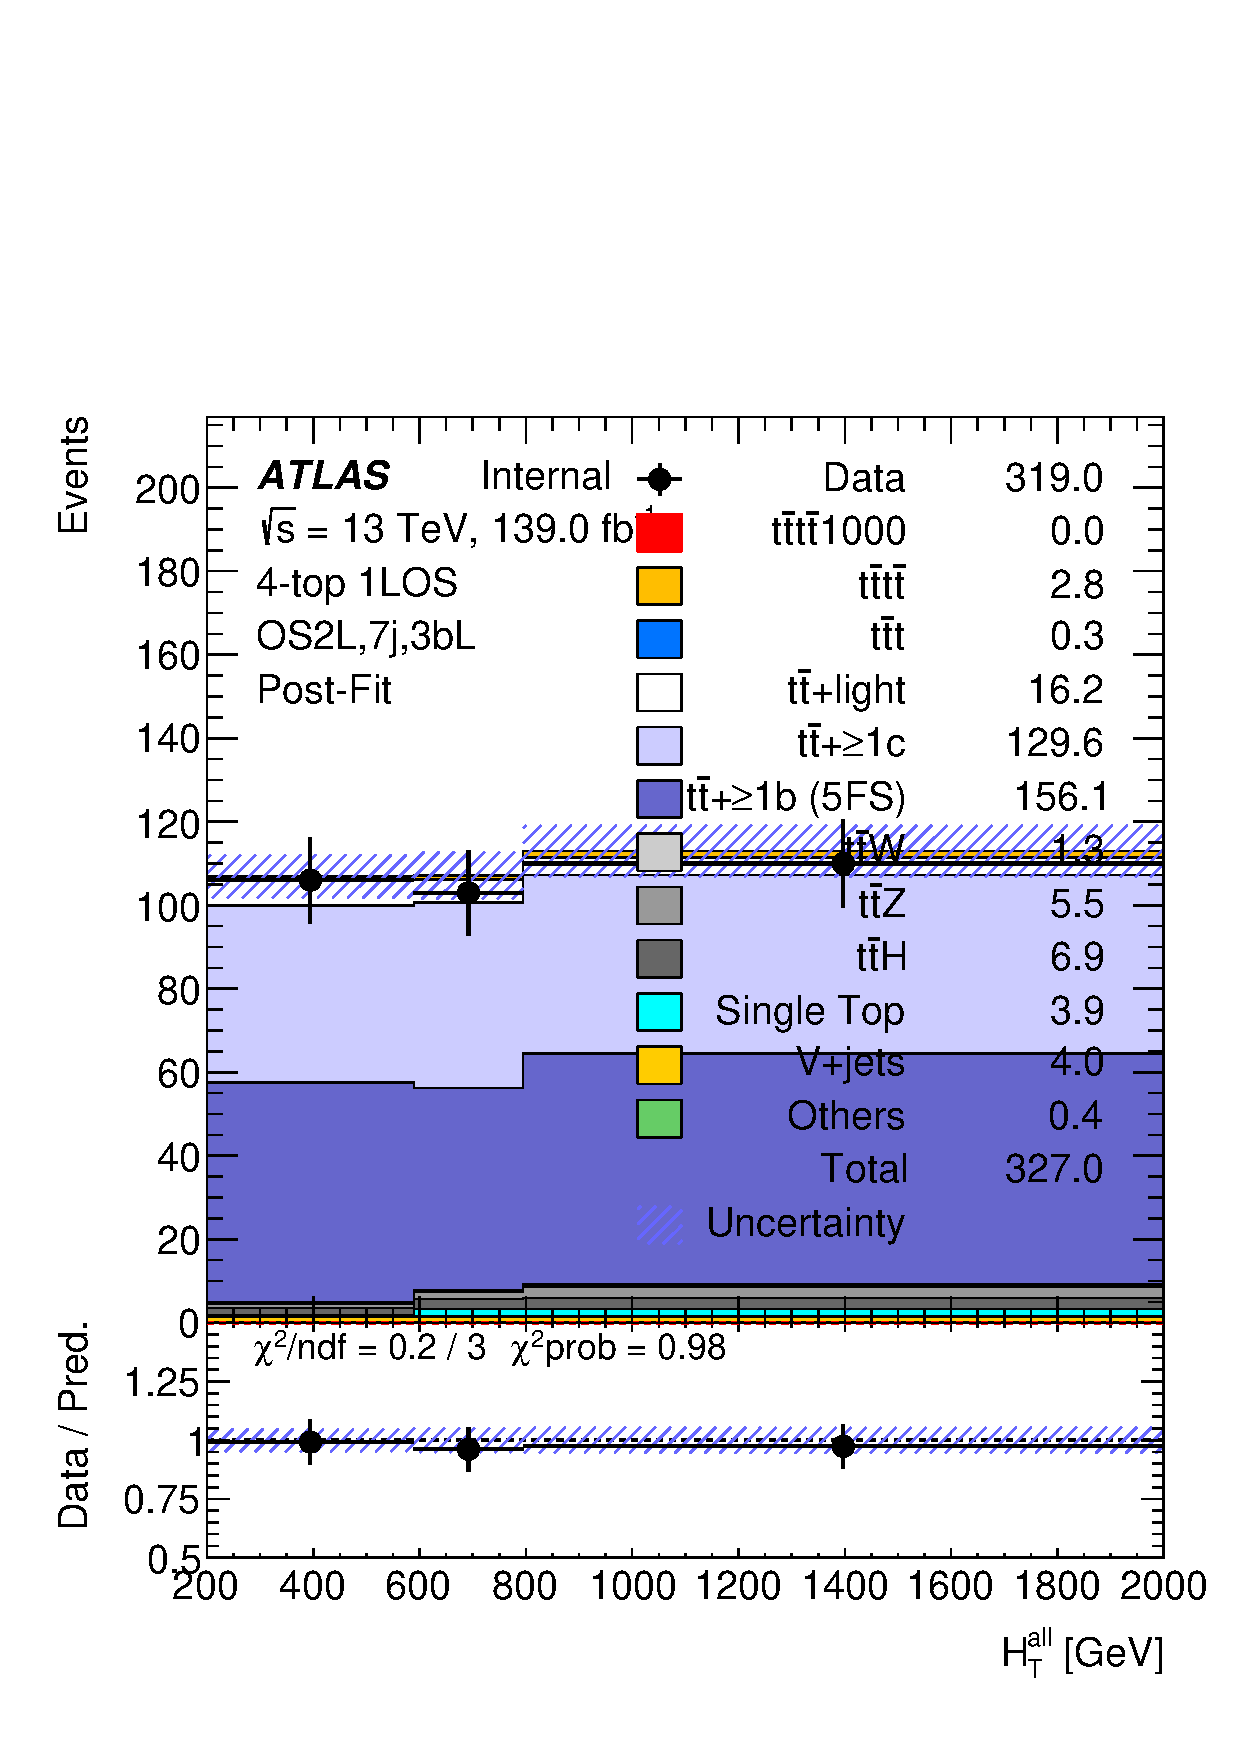
\includegraphics[width=0.31 \textwidth]{figures/fits/GNN/1000/all/data_unblindedBonly/Plots/os2l_7j3bL_postFit.pdf} &
        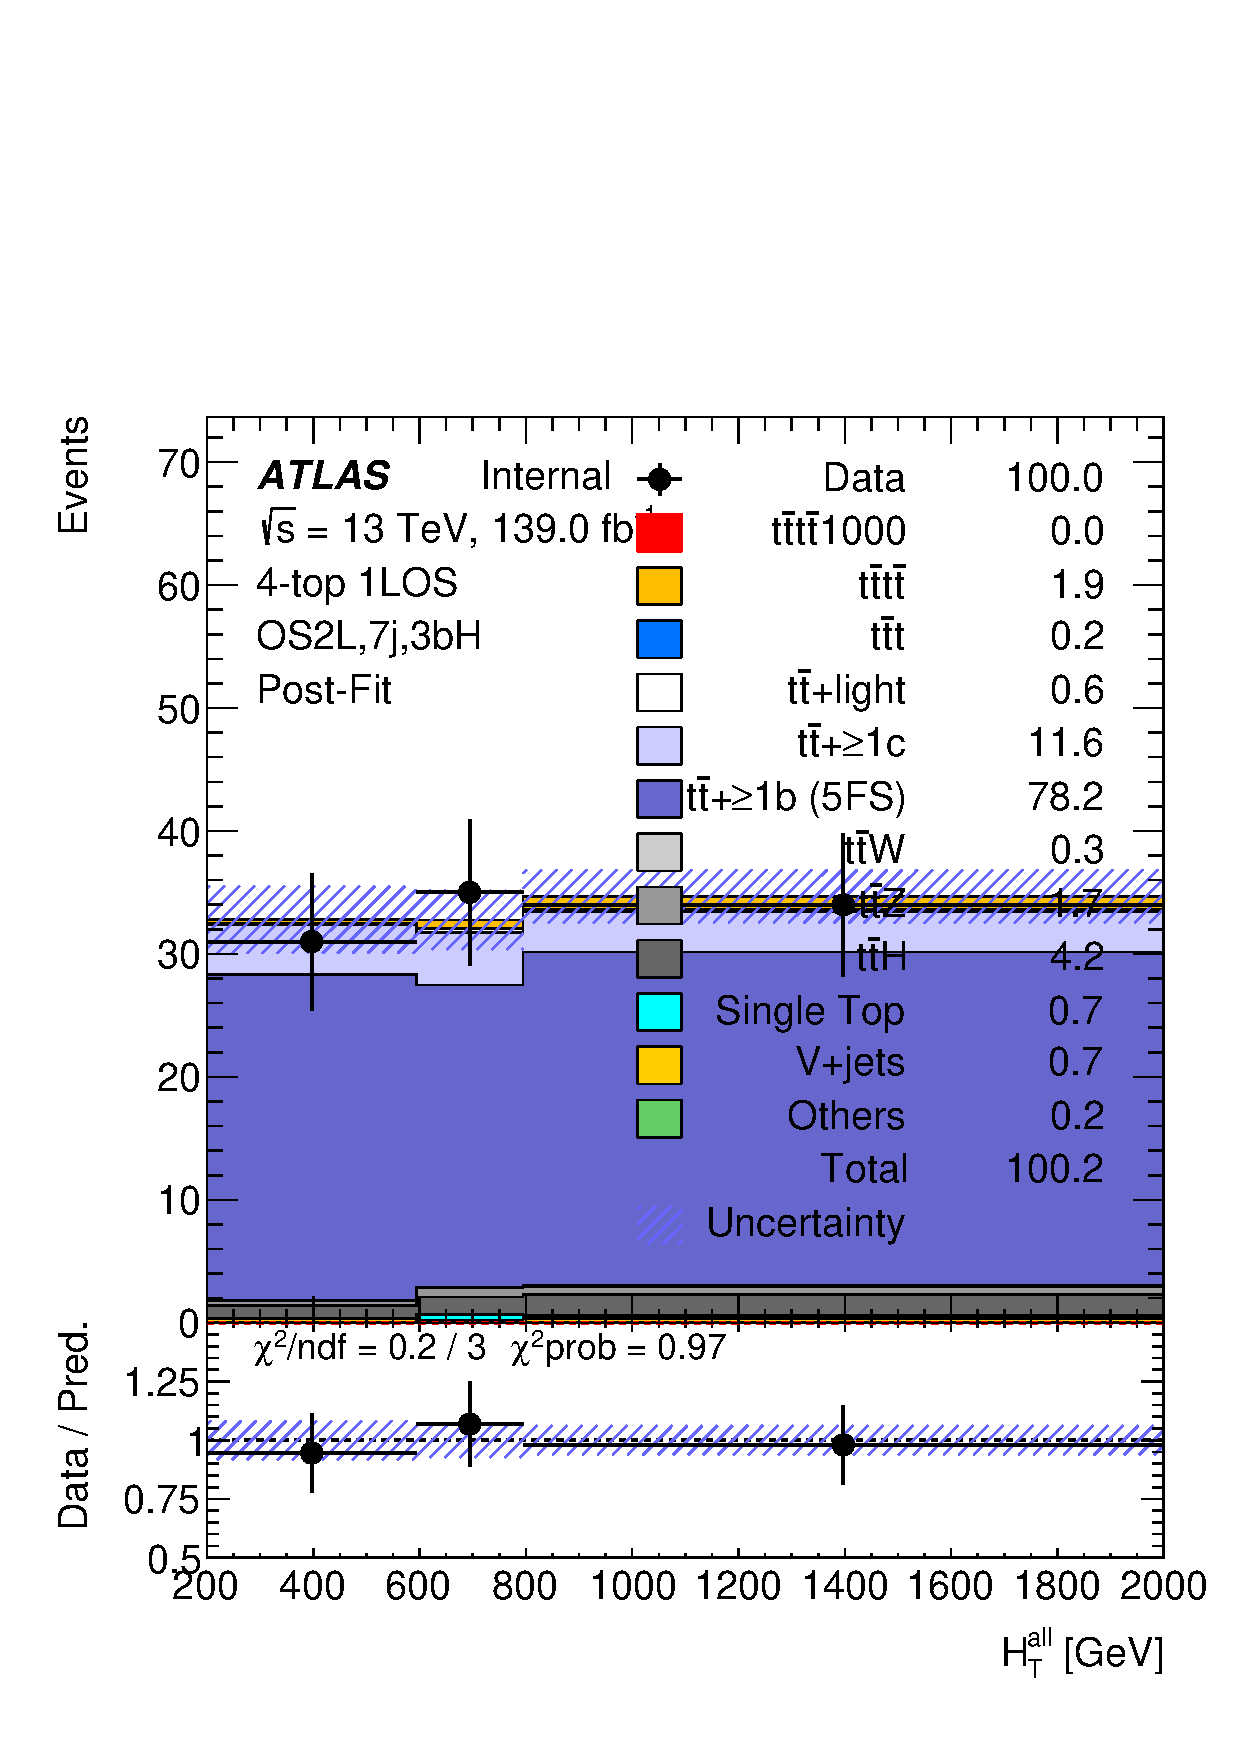
\includegraphics[width=0.31 \textwidth]{figures/fits/GNN/1000/all/data_unblindedBonly/Plots/os2l_7j3bH_postFit.pdf} &
        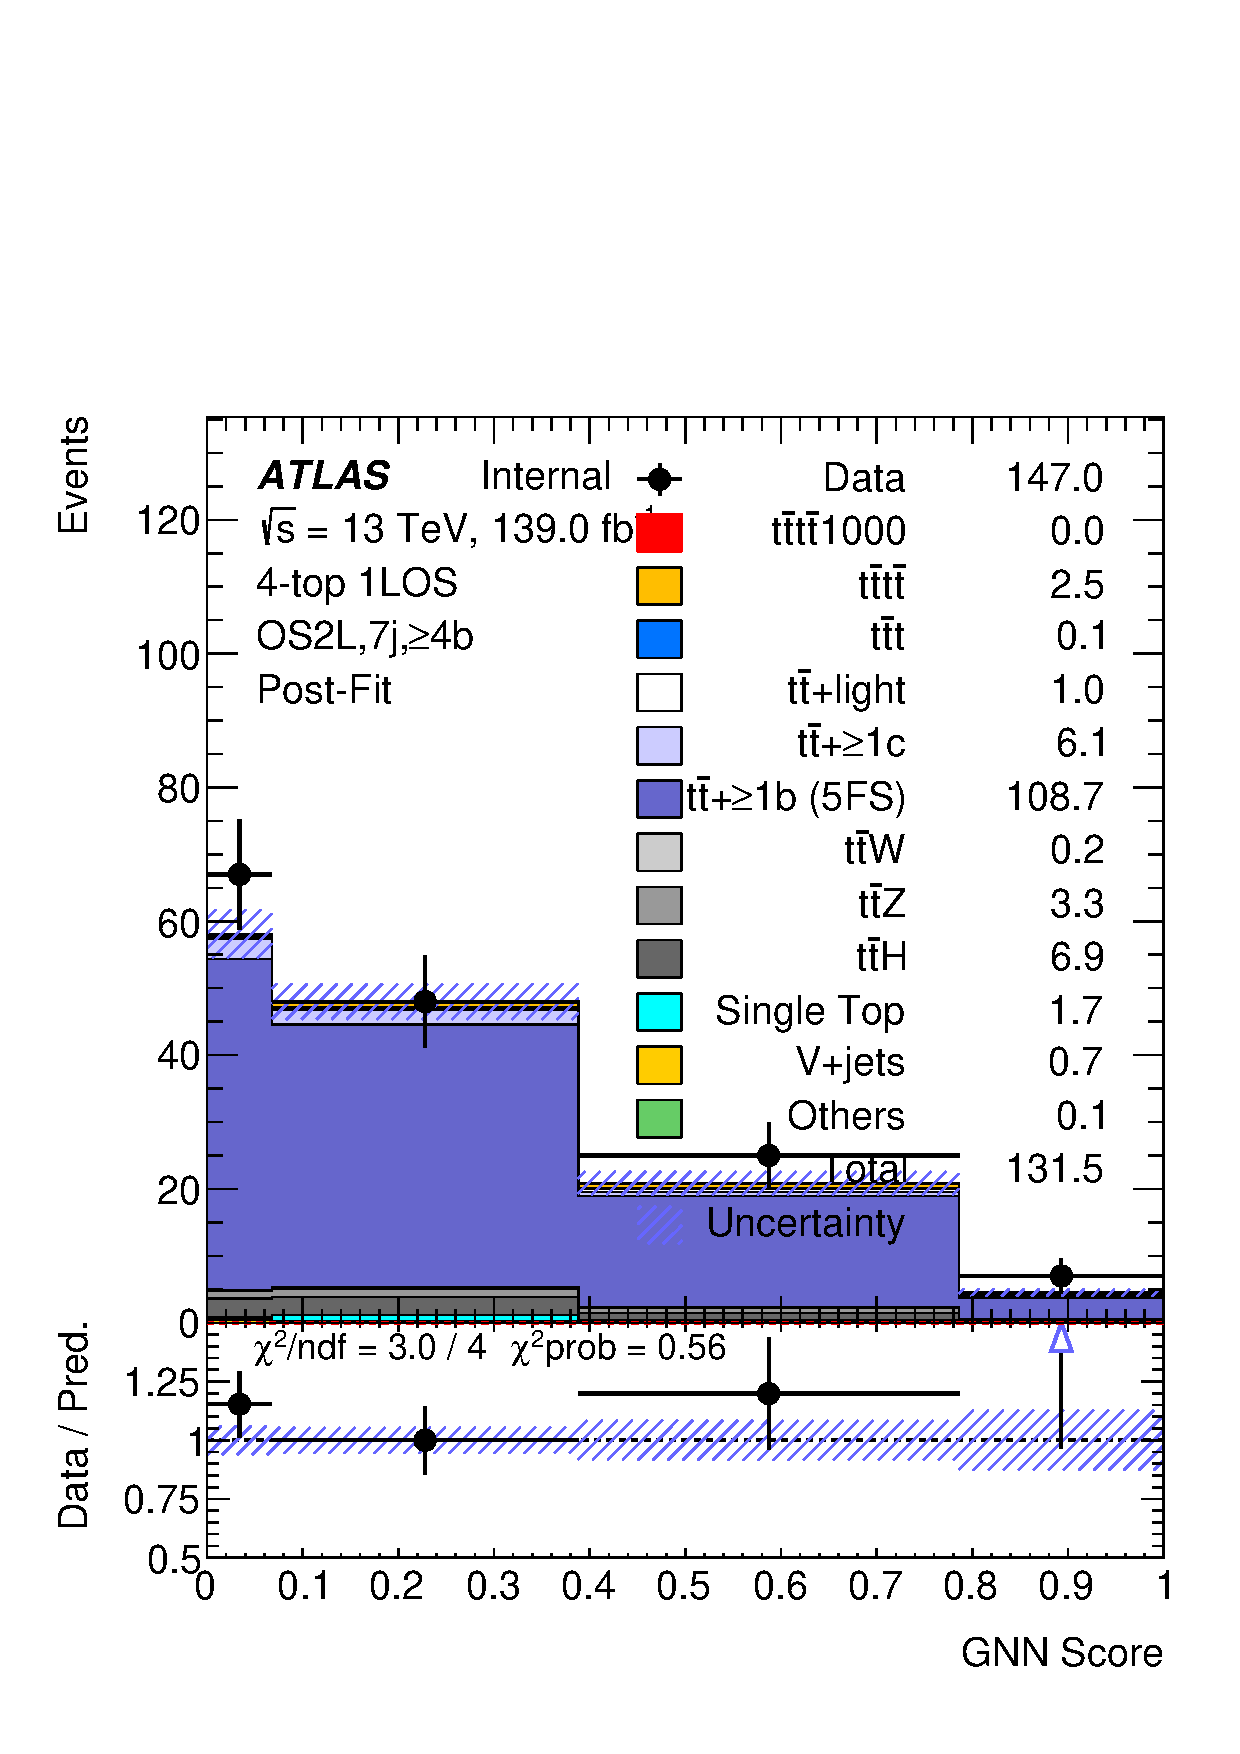
\includegraphics[width=0.31 \textwidth]{figures/fits/GNN/1000/all/data_unblindedBonly/Plots/os2l_7jge4b_postFit.pdf} \\

        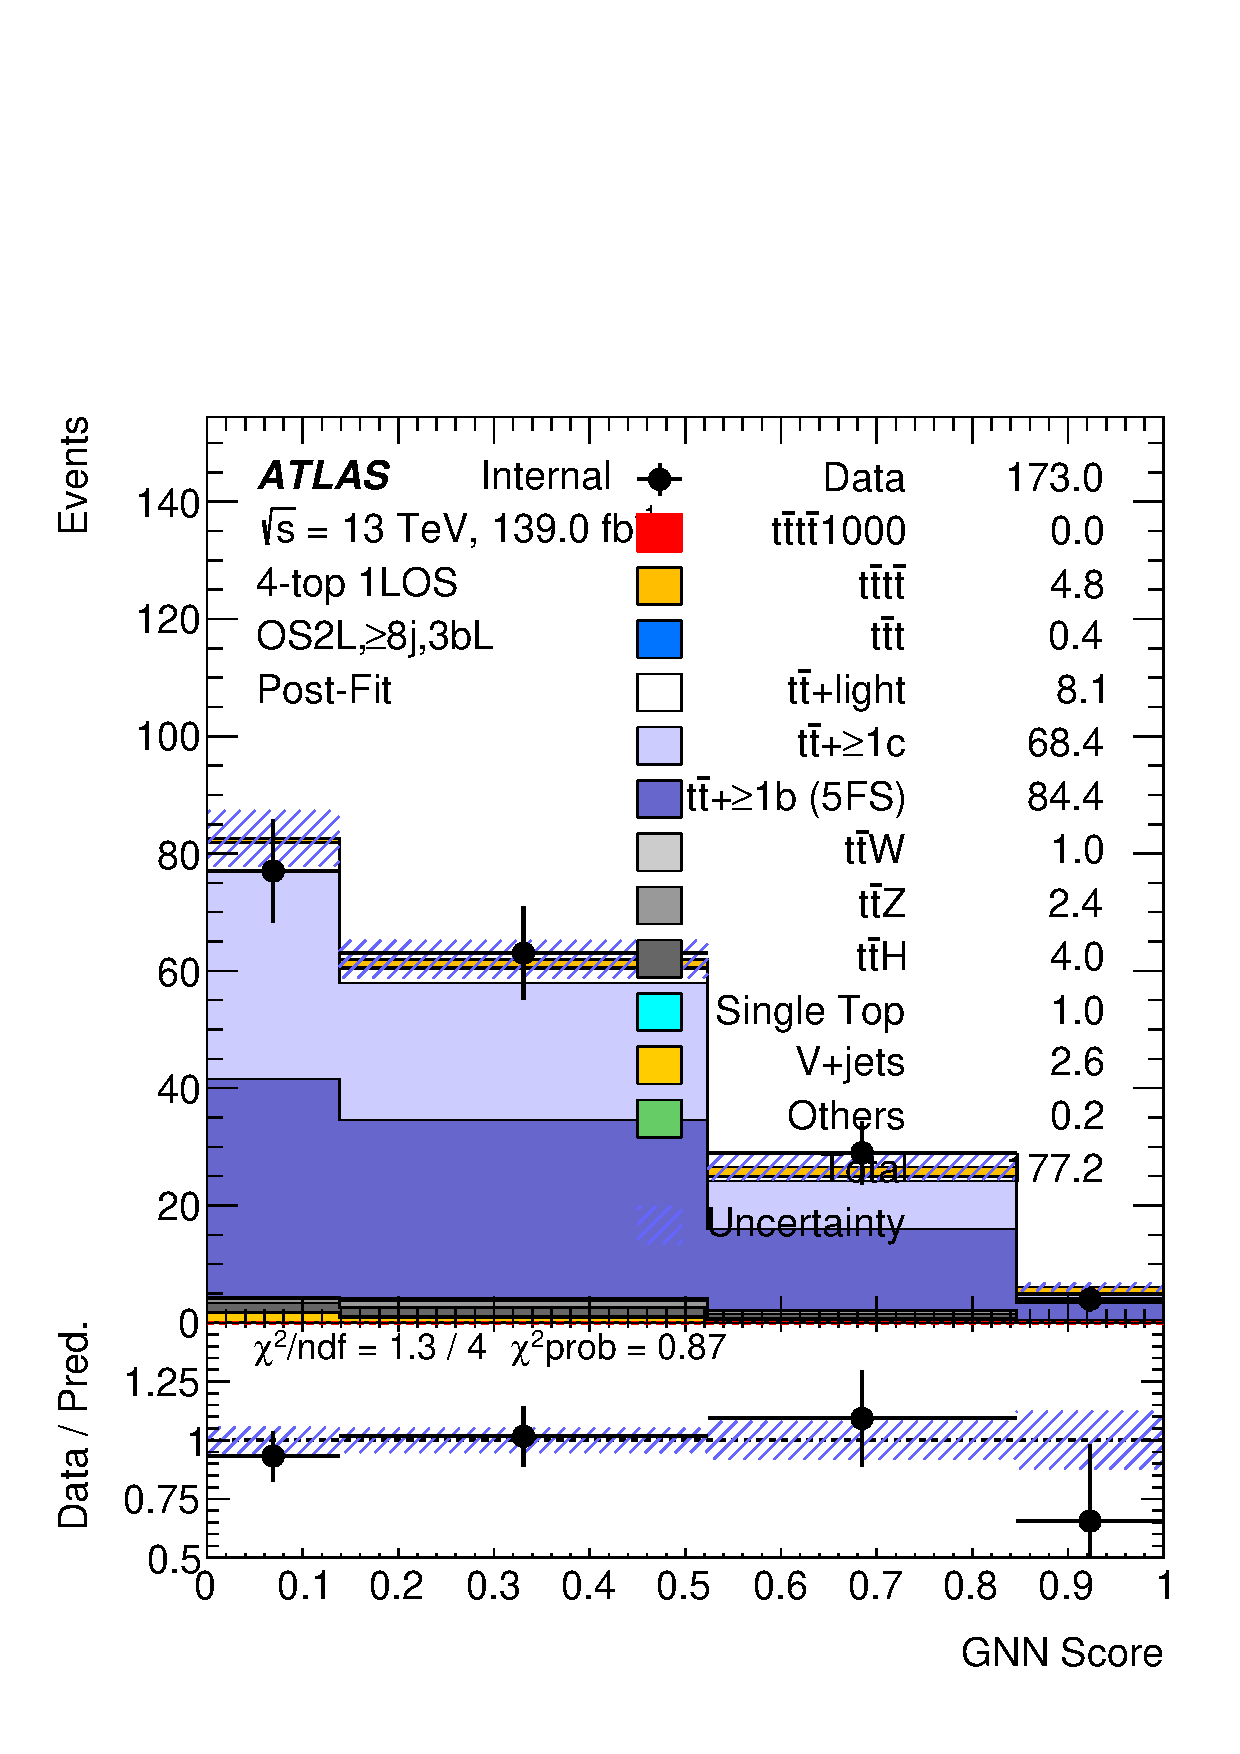
\includegraphics[width=0.31 \textwidth]{figures/fits/GNN/1000/all/data_unblindedBonly/Plots/os2l_ge8j3bL_postFit.pdf} &
        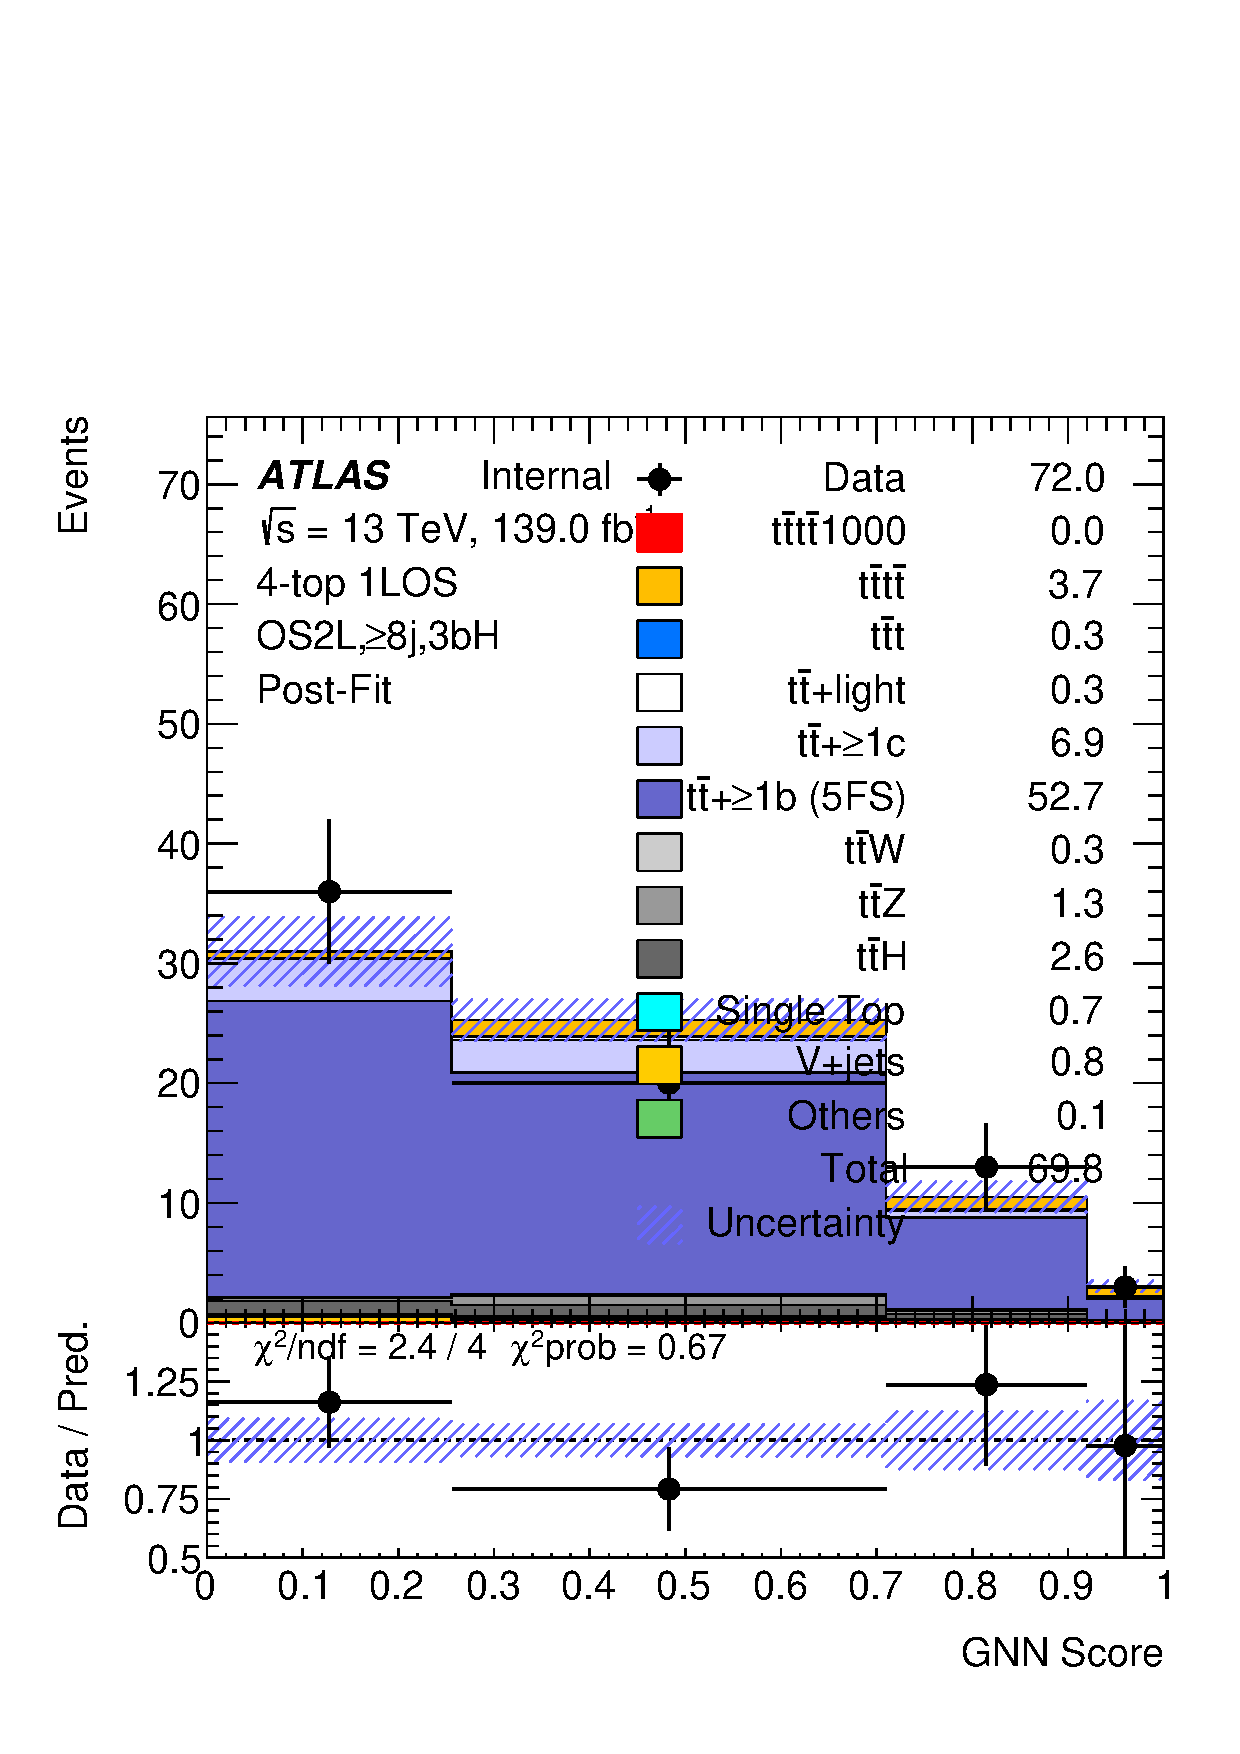
\includegraphics[width=0.31 \textwidth]{figures/fits/GNN/1000/all/data_unblindedBonly/Plots/os2l_ge8j3bH_postFit.pdf} &
        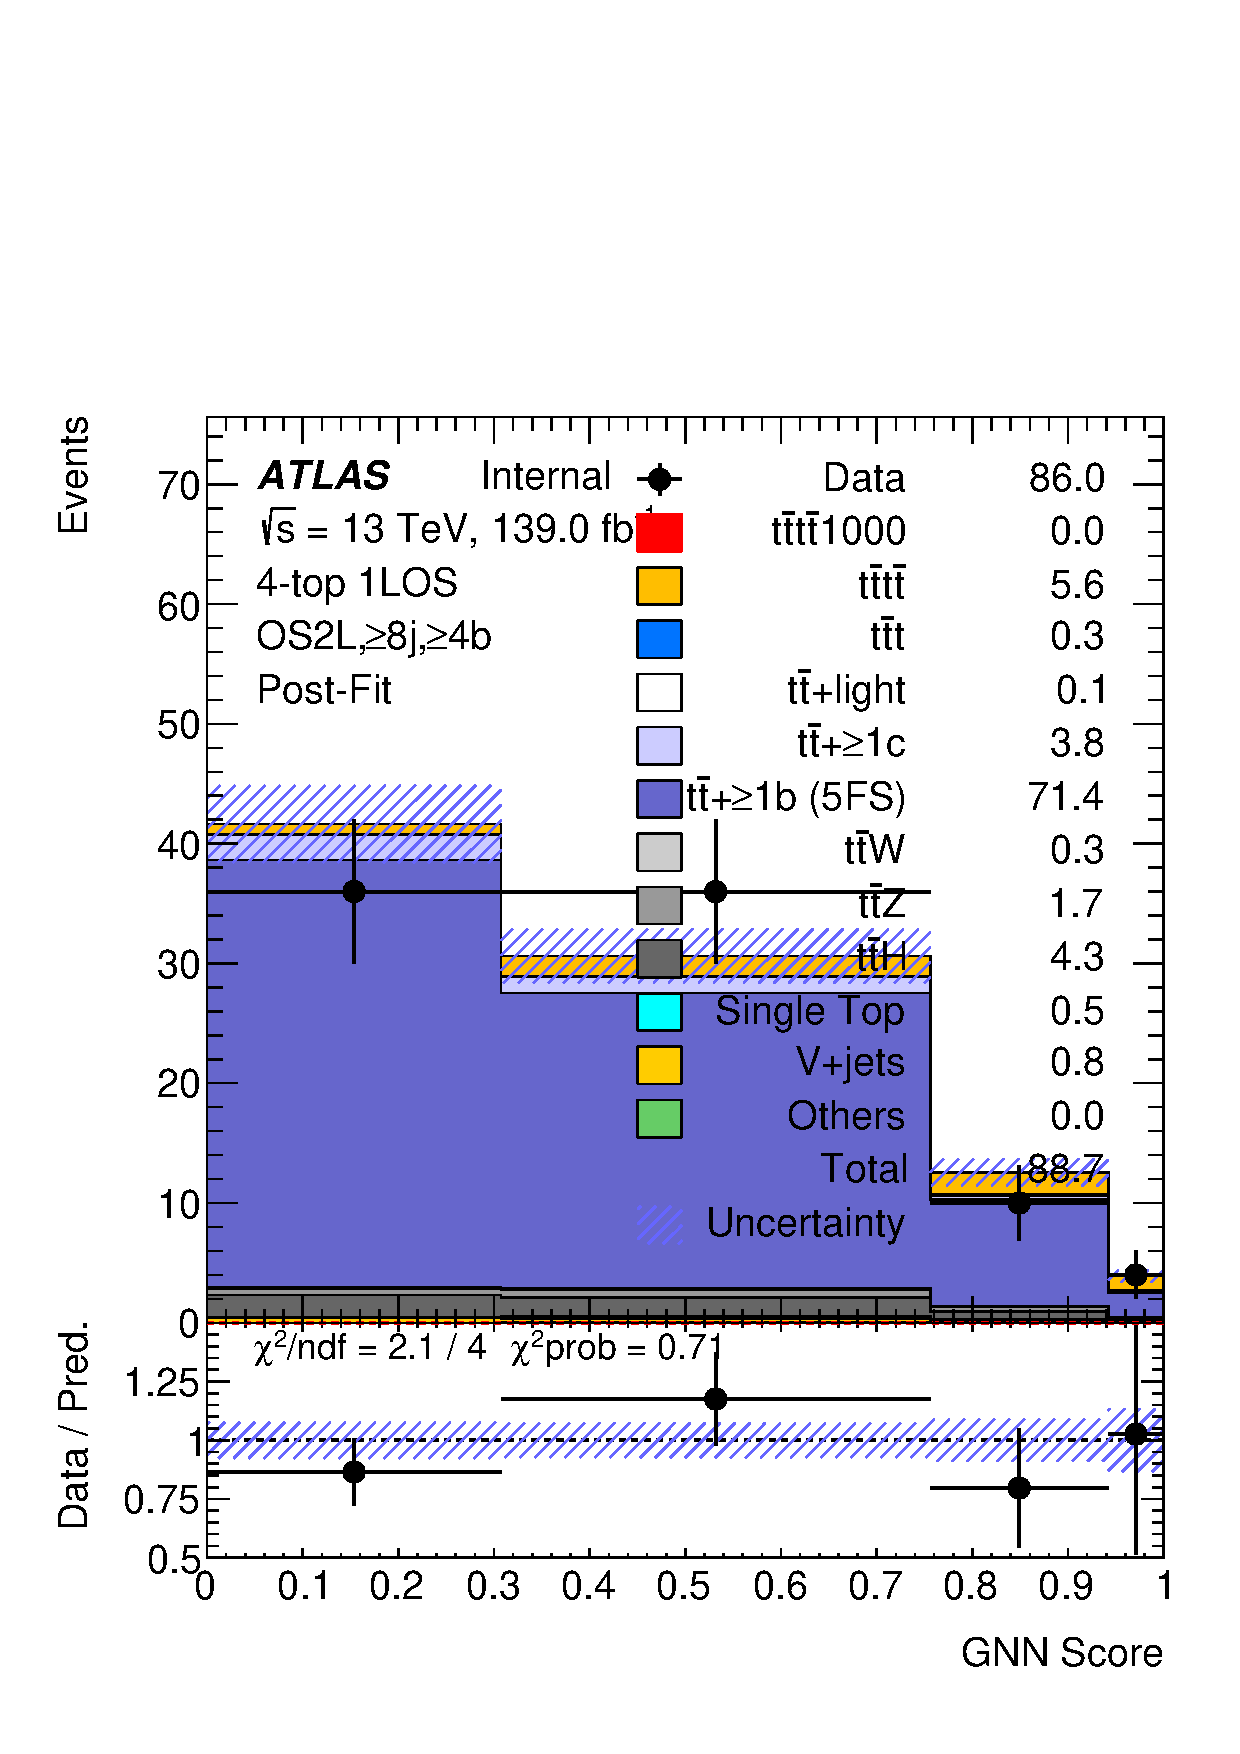
\includegraphics[width=0.31 \textwidth]{figures/fits/GNN/1000/all/data_unblindedBonly/Plots/os2l_ge8jge4b_postFit.pdf} \\
        \end{tabular}
        \caption{\label{fig:Postfit_Yields_2L_1000GeV}Post-fit distributions for 2LOS regions associated with different signal and background samples, compared with data yields for mH = 1000 GeV. The fit is done using all regions (1L+2L). The same plots for mH = 400 GeV are shown in Figure \ref{fig:Postfit_Yields_2L}.}
\end{center}
\end{figure}

\begin{figure}[htbp!]
        \centering
        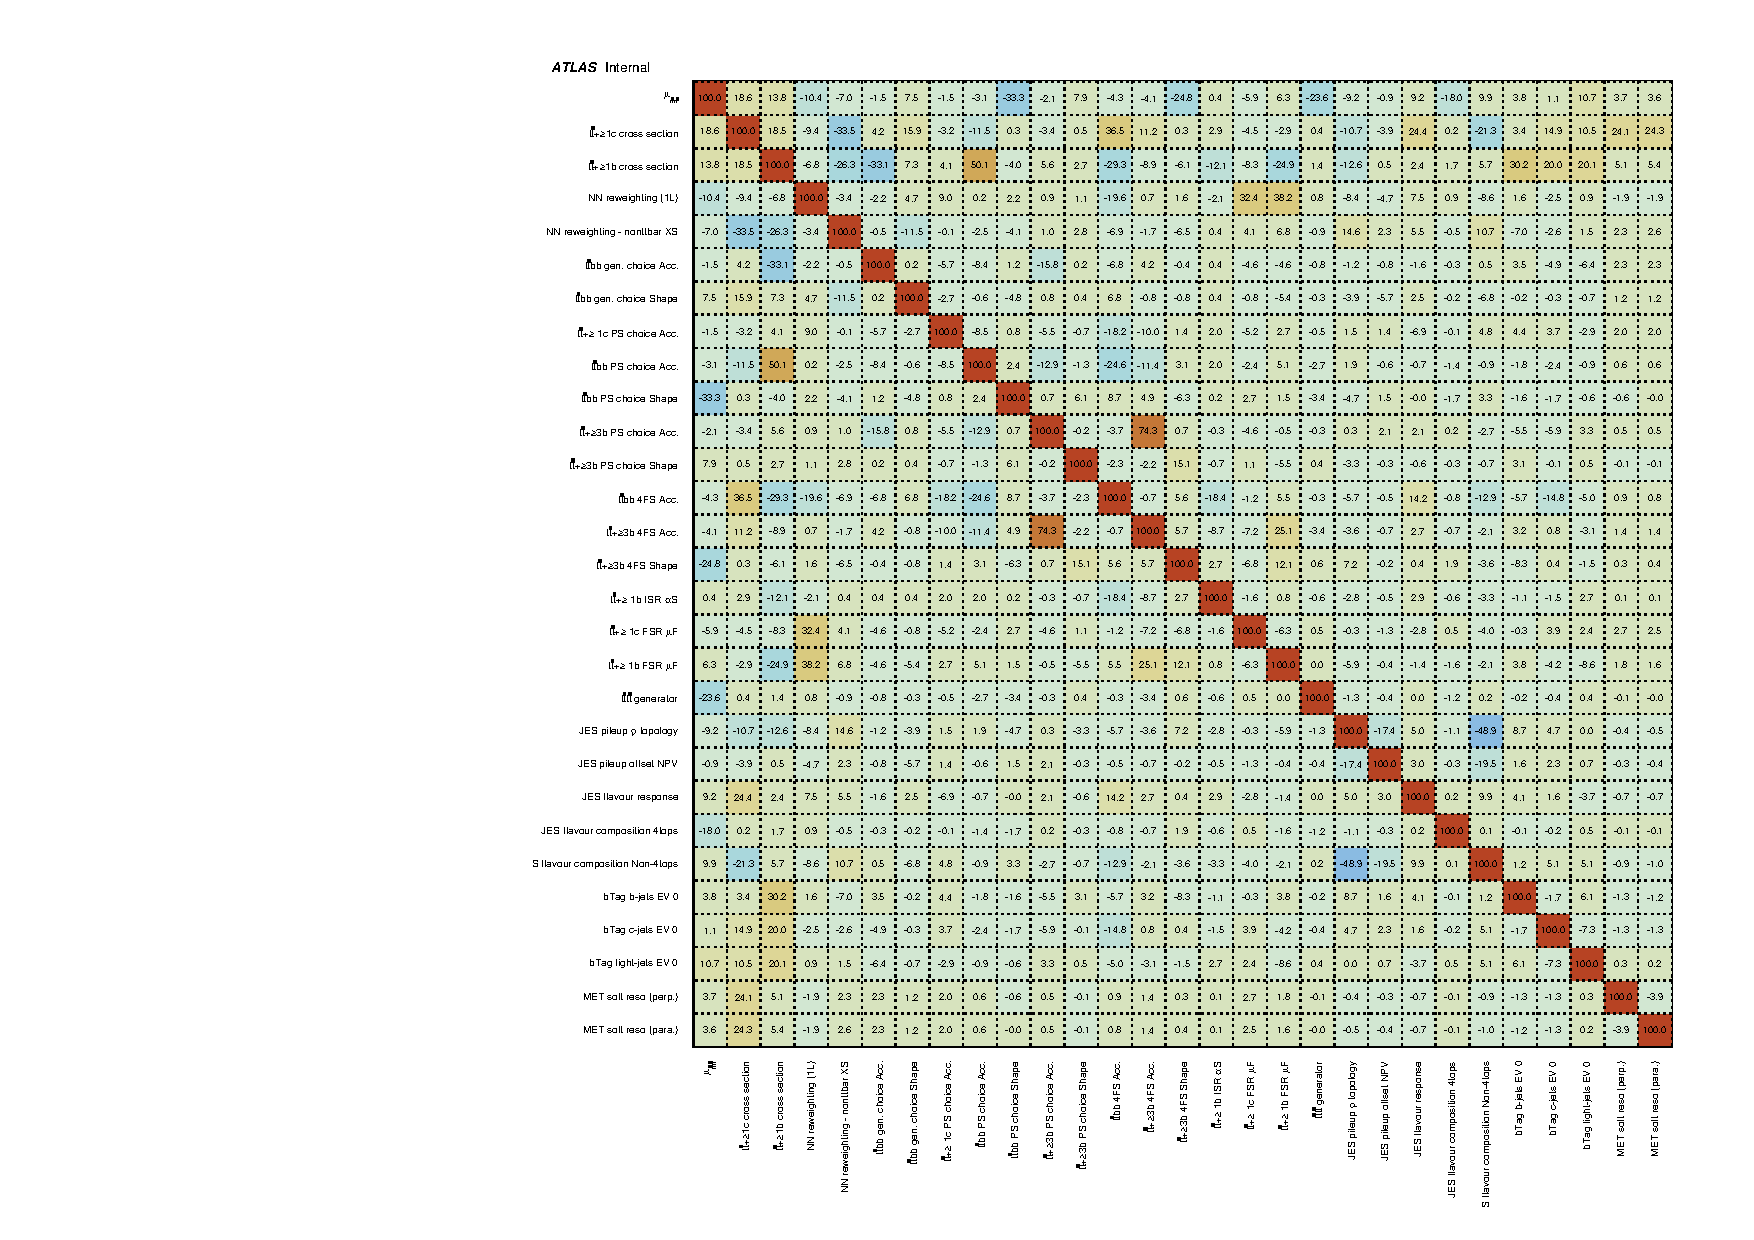
\includegraphics[width=\linewidth]{figures/fits/GNN/1000/1L/asimov/CorrMatrix.pdf}
        \caption{\label{fig:Corr_mH1000_Asimov_1L}Correlation matrix for the 1L Asimov fit for mH = 1000 GeV}
\end{figure}

\begin{figure}[htbp!]
        \centering
        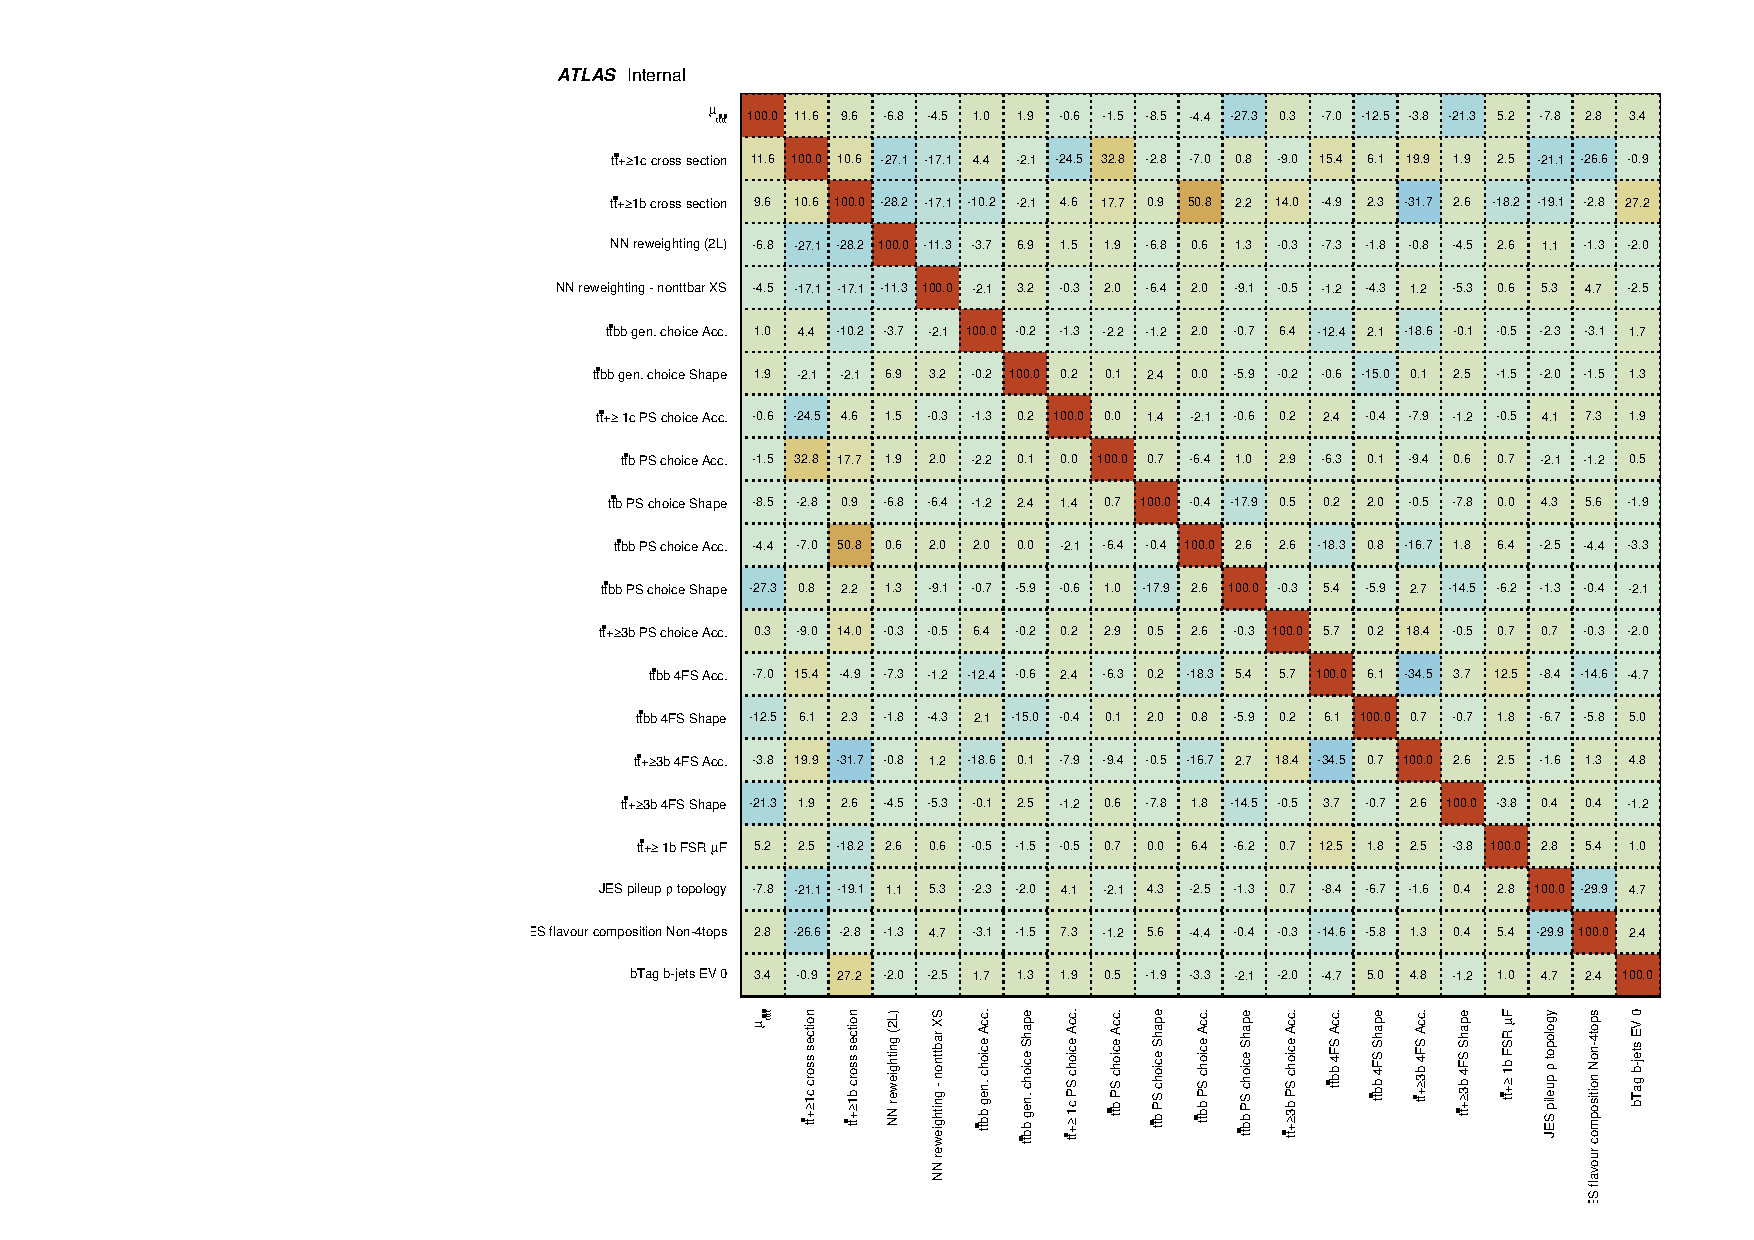
\includegraphics[width=\linewidth]{figures/fits/GNN/1000/2L/asimov/CorrMatrix.pdf}
        \caption{\label{fig:Corr_mH1000_Asimov_2L}Correlation matrix for the 2LOS Asimov fit for mH = 1000 GeV}
\end{figure}

\begin{figure}[htbp!]
        \centering
        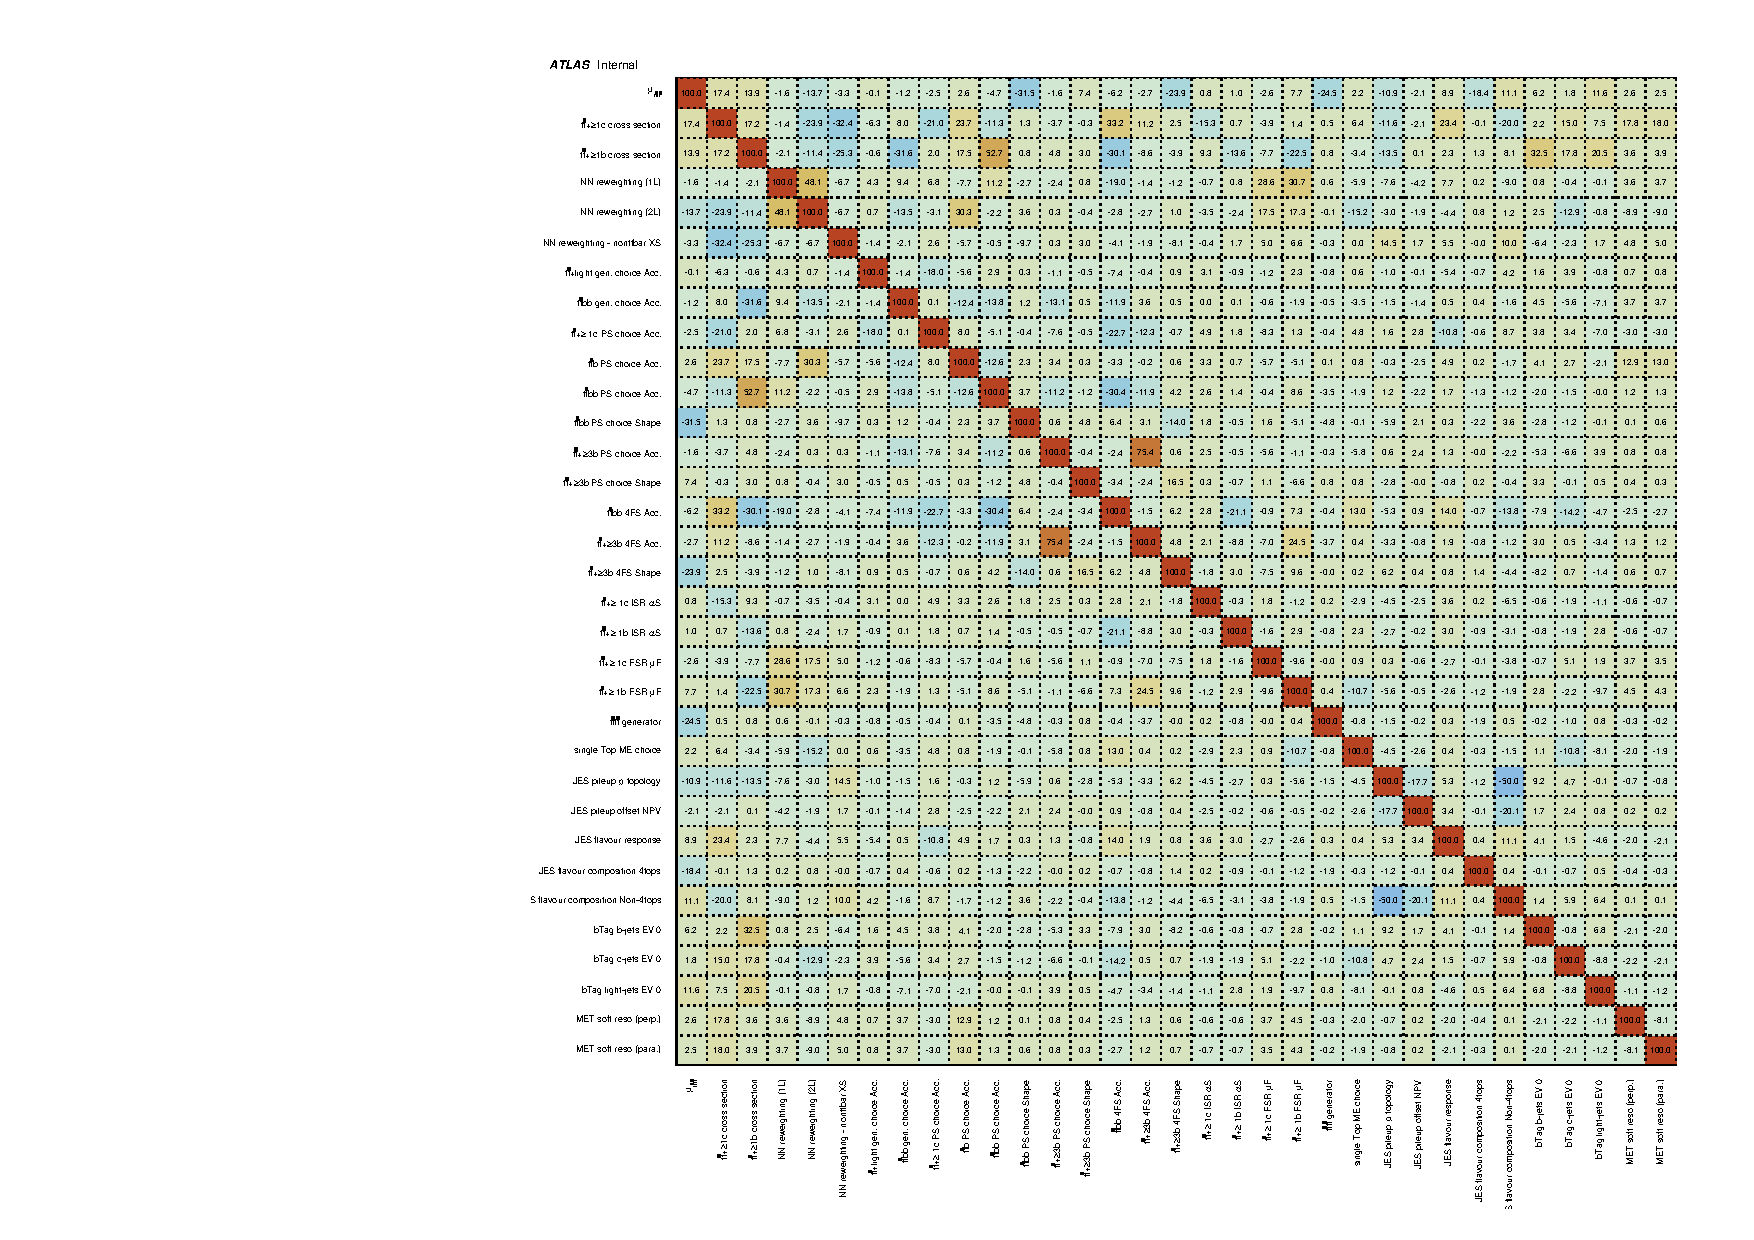
\includegraphics[width=\linewidth]{figures/fits/GNN/1000/all/asimov/CorrMatrix.pdf}
        \caption{\label{fig:Corr_mH1000_Asimov_all}Correlation matrix for the 1L/2LOS combined Asimov fit for mH = 1000 GeV}
\end{figure}


\begin{figure}[htbp!]
        \centering
        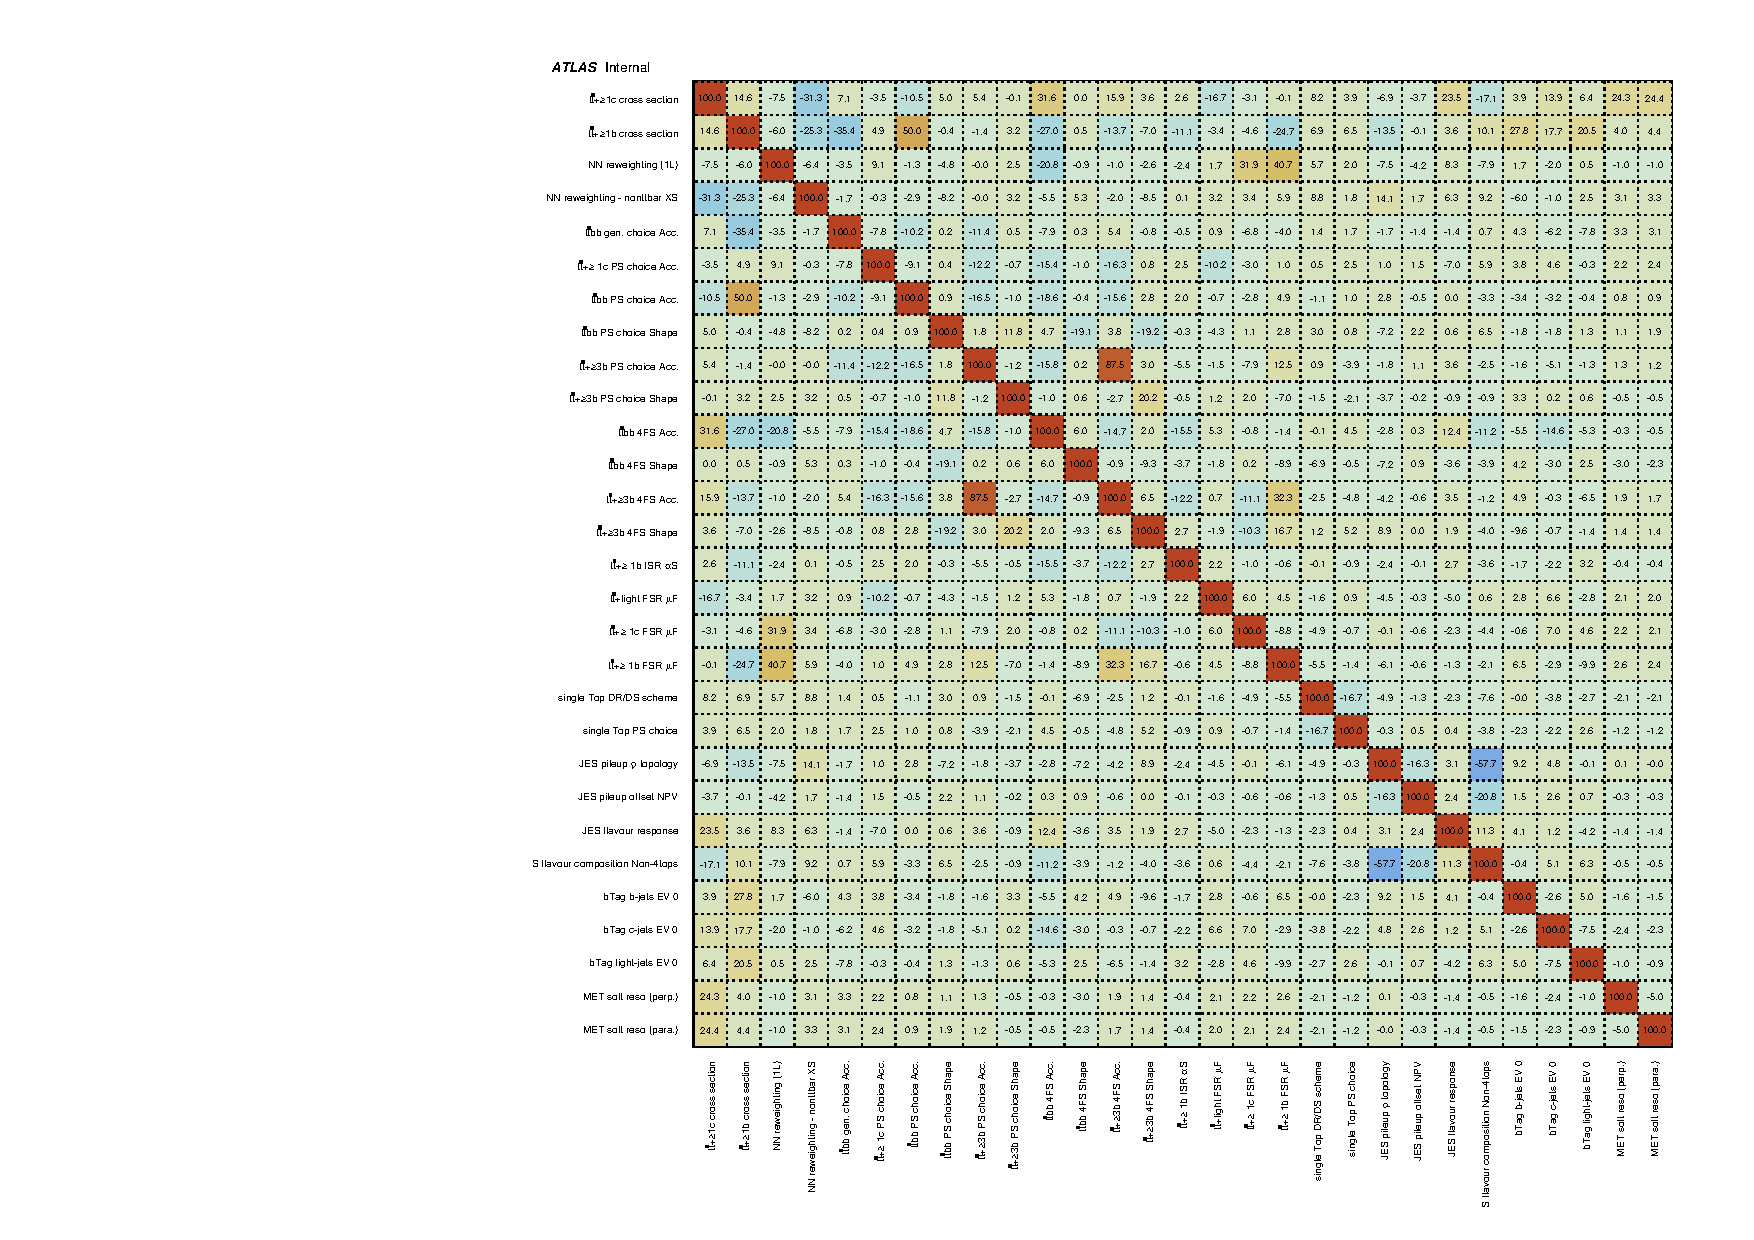
\includegraphics[width=\linewidth]{figures/fits/GNN/1000/1L/data_unblindedBonly/CorrMatrix.pdf}
        \caption{\label{fig:Corr_mH1000_Data_1L}Correlation matrix for the 1L blinded data fit for mH = 1000 GeV}
\end{figure}

\begin{figure}[htbp!]
        \centering
        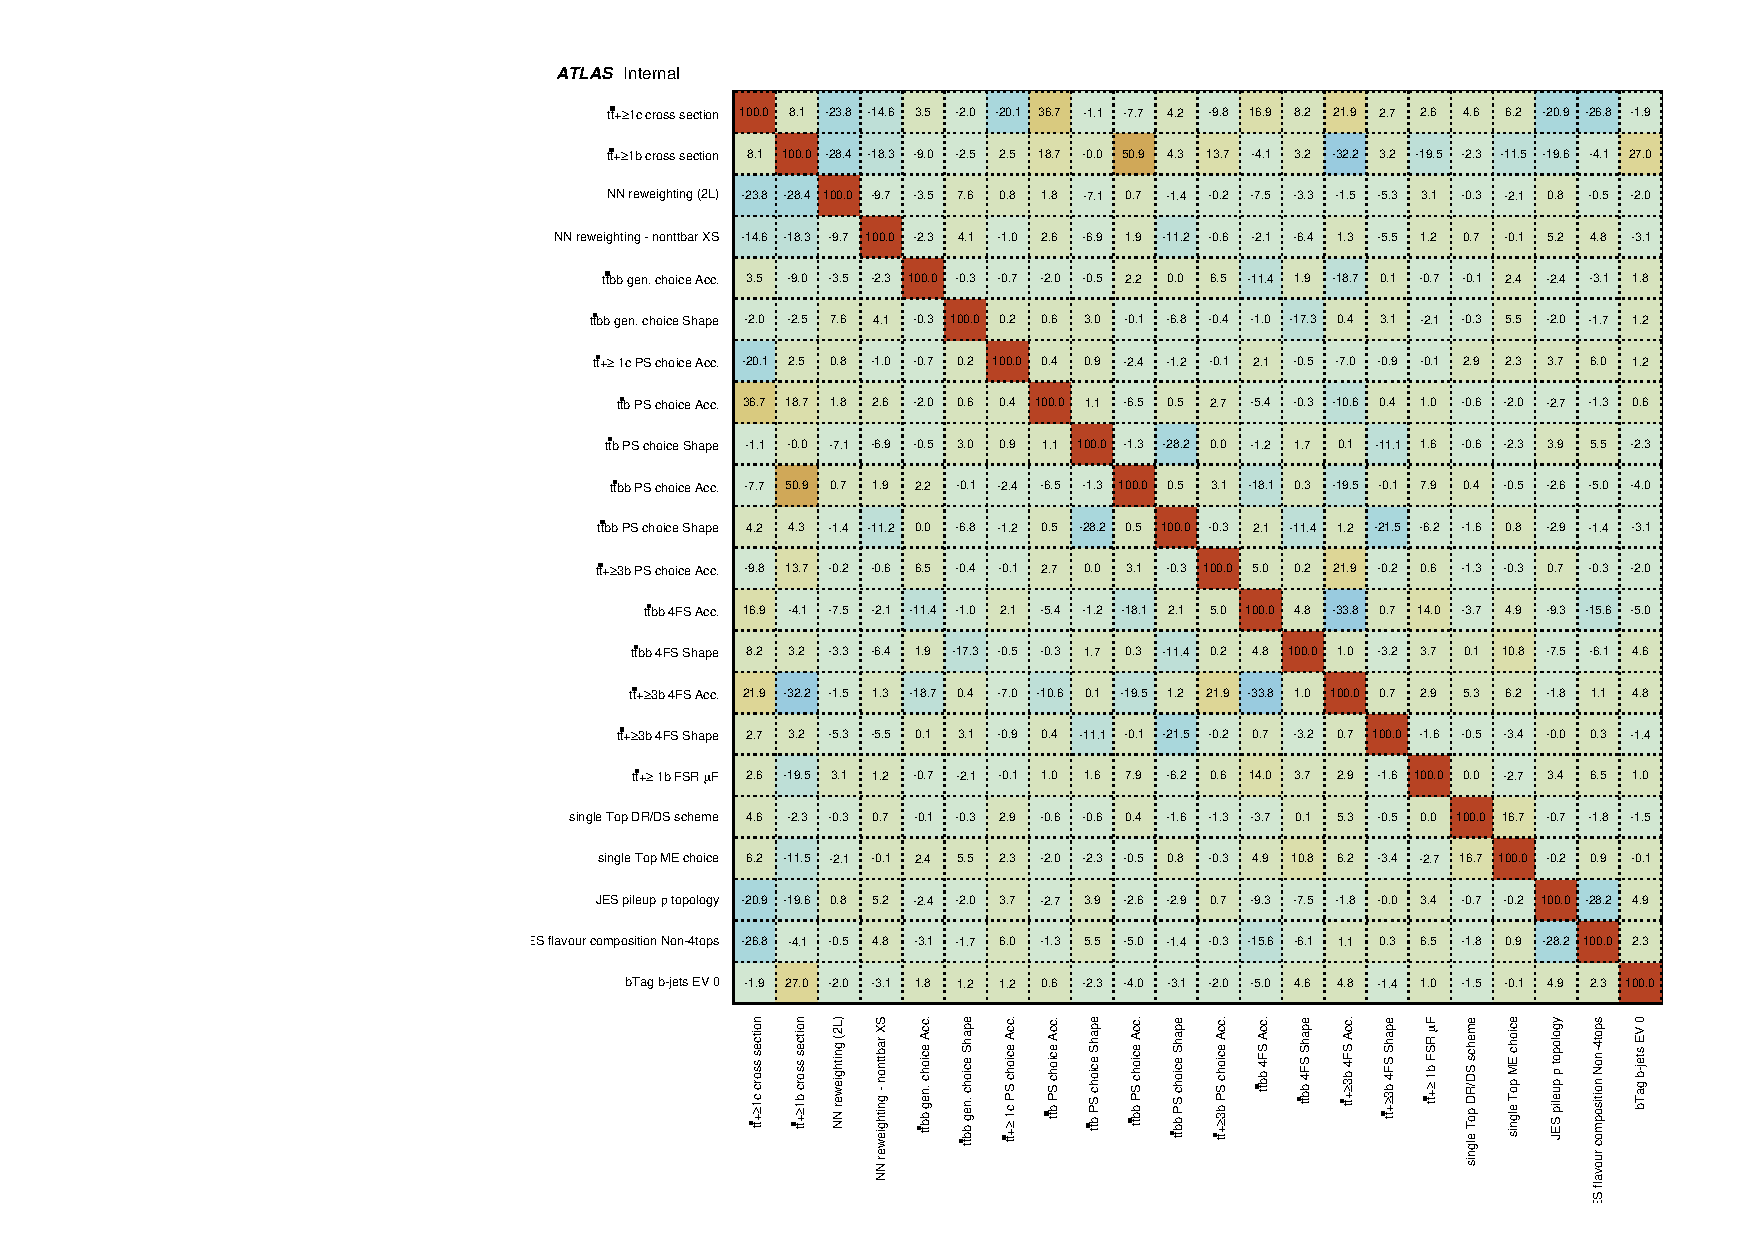
\includegraphics[width=\linewidth]{figures/fits/GNN/1000/2L/data_unblindedBonly/CorrMatrix.pdf}
        \caption{\label{fig:Corr_mH1000_Data_2L}Correlation matrix for the 2LOS blinded data fit for mH = 1000 GeV}
\end{figure}

\begin{figure}[htbp!]
        \centering
        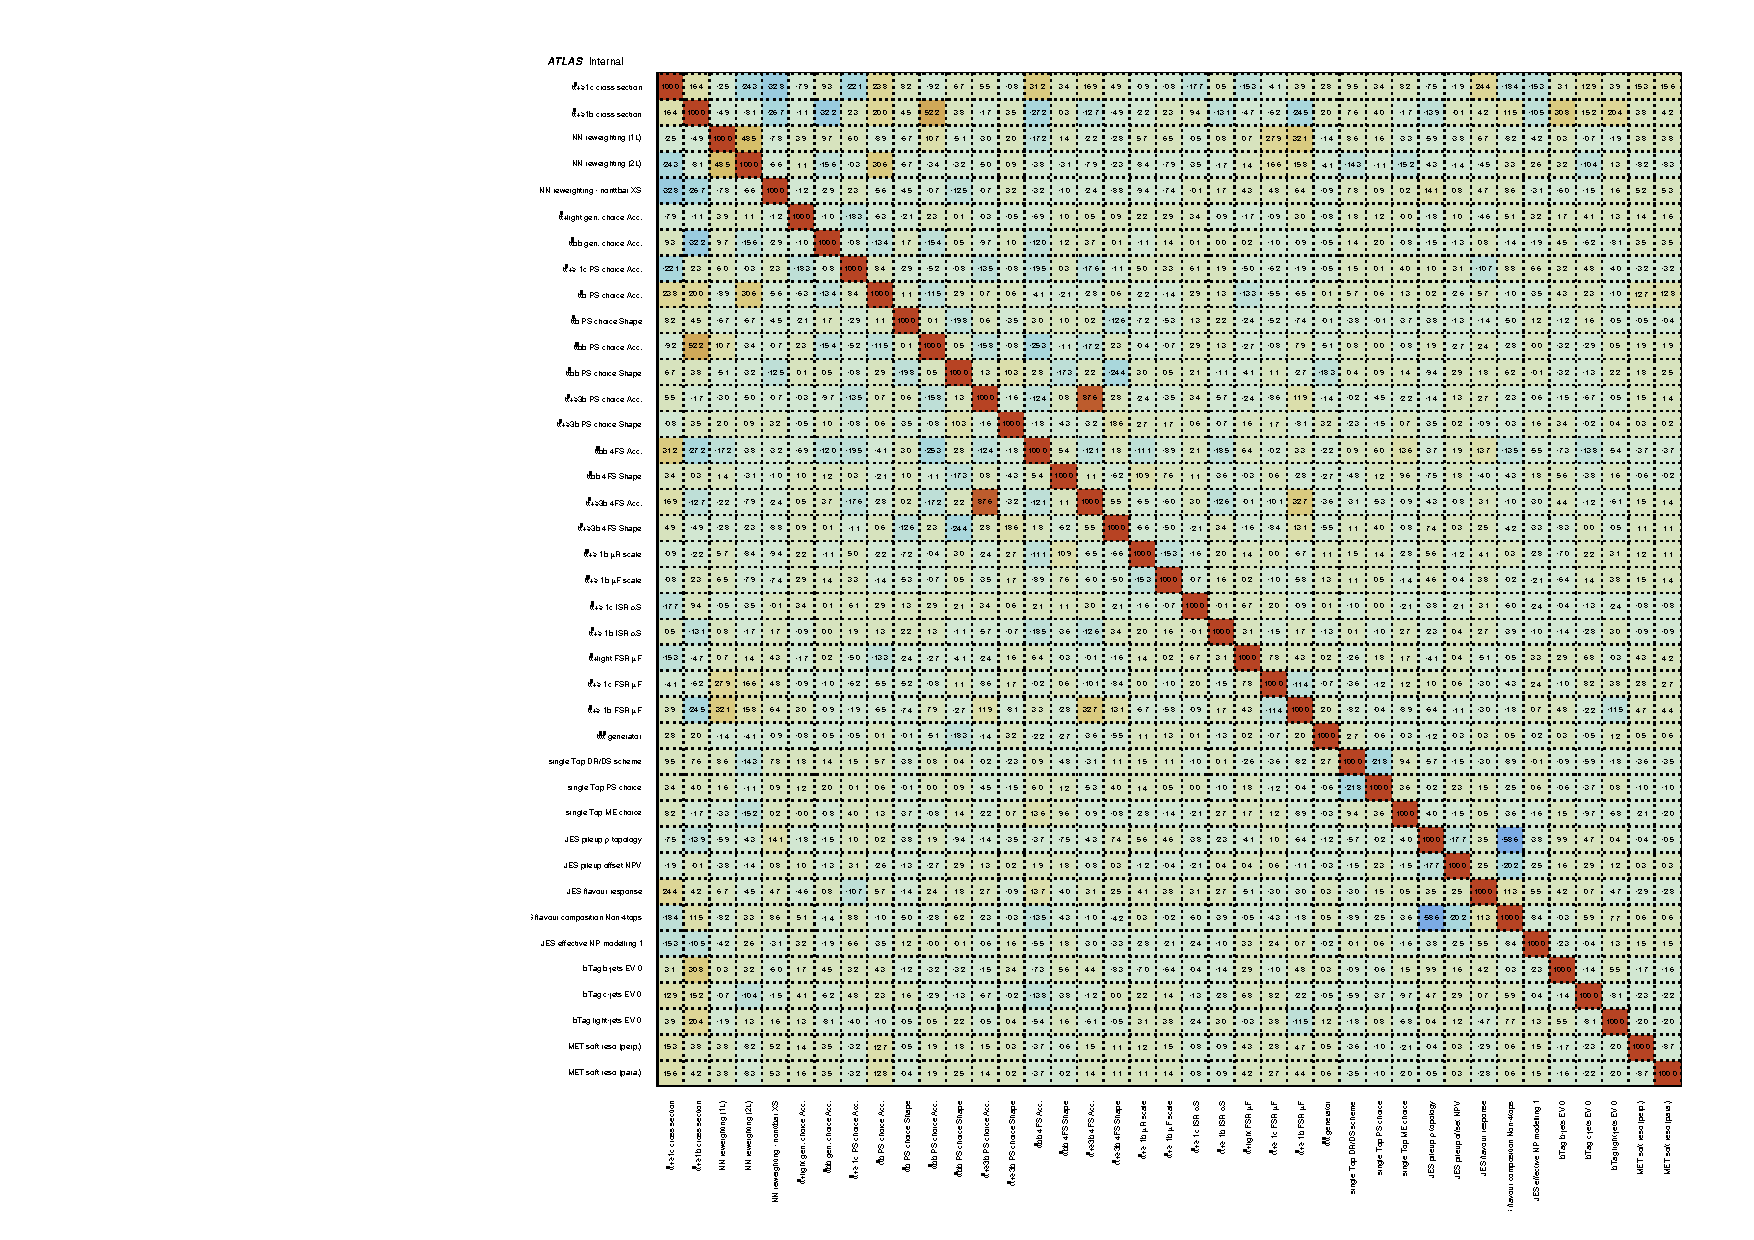
\includegraphics[width=\linewidth]{figures/fits/GNN/1000/all/data_unblindedBonly/CorrMatrix.pdf}
        \caption{\label{fig:Corr_mH1000_Data_all}Correlation matrix for the 1L/2LOS combined blinded data fit for mH = 1000 GeV}
\end{figure}
